%
% The Quantum Internet - A Vision for the Future
%

\documentclass[aps,rmp,twocolumn,amsmath,amssymb,nofootinbib,superscriptaddress,longbibliography,floatfix]{revtex4-1}

\usepackage[pdftex]{graphicx}
\usepackage{mathrsfs}
\usepackage[colorlinks]{hyperref}
\usepackage{url}
\usepackage[dvipsnames]{xcolor}
\usepackage[]{qcircuit}

\newcommand{\comment}[1]{{\color{blue}{\textbf{#1}}}}

\newcommand{\bra}[1]{\langle#1|}
\newcommand{\ket}[1]{|#1\rangle}

\newcommand{\comment}[1]{{\color{blue}{\textbf{#1}}}}
\newcommand{\peter}[1]{{\color{Aquamarine}{#1}}}
%\newcommand{\peter}[1]{{\color{black}{#1}}}
\newcommand{\jonny}[1]{{\color{Orchid}{#1}}}
\newcommand{\ryan}[1]{{\color{YellowGreen}{#1}}}
\newcommand{\chaoyang}[1]{{\color{Apricot}{#1}}}
\newcommand{\zuen}[1]{{\color{Bittersweet}{\textbf{#1}}}}
\newcommand{\mick}[1]{{\color{Lavender}{\textbf{#1}}}}
\newcommand{\sihui}[1]{{\color{Emerald}{\textbf{#1}}}}

\renewcommand{\tablename}{ALG.}

\newtheorem{definition}{Definition}

\begin{document}

%
% Title
%

\title{The Quantum Internet -- A Vision for the Future}

%
% Authors
%

\author{Peter P. Rohde}
\email[To whom correspondence should be addressed: ]{dr.rohde@gmail.com}
\homepage{http://www.peterrohde.org}
\affiliation{Centre for Quantum Software \& Information (CQSI), Faculty of Engineering \& Information Technology, University of Technology Sydney, NSW 2007, Australia}

\author{Zu-En Su}
\affiliation{Hefei National Laboratory for Physical Sciences at Microscale and Department of Modern Physics, University of Science and Technology of China, Hefei, Anhui 230026, China}
\affiliation{CAS Centre for Excellence and Synergetic Innovation Centre in Quantum Information and Quantum Physics, University of Science and Technology of China, Hefei, Anhui 230026, China}
\affiliation{CAS-Alibaba Quantum Computing Laboratory, Shanghai 201315, China}

\author{He-Liang Huang}
\affiliation{Hefei National Laboratory for Physical Sciences at Microscale and Department of Modern Physics, University of Science and Technology of China, Hefei, Anhui 230026, China}
\affiliation{CAS Centre for Excellence and Synergetic Innovation Centre in Quantum Information and Quantum Physics, University of Science and Technology of China, Hefei, Anhui 230026, China}
\affiliation{CAS-Alibaba Quantum Computing Laboratory, Shanghai 201315, China}

\author{Samuel I. Marks}
\affiliation{Sydney Medical School, University of Sydney, Australia}

\author{Ryan L. Mann}
\affiliation{Centre for Quantum Software \& Information (CQSI), Faculty of Engineering \& Information Technology, University of Technology Sydney, NSW 2007, Australia}

%\author{Jonathan P. Olson}
%\affiliation{Department of Chemistry \& Chemical Biology, Harvard University, Cambridge MA 02138, USA}

\author{William J. Munro}
\affiliation{NTT Basic Research Laboratories, 3-1 Morinosato-Wakamiya, Atsugi, Kanagawa 243-0198, Japan}
\affiliation{National Institute of Informatics, 2-1-2 Hitotsubashi, Chiyoda-ku, Tokyo 101-8430, Japan}

\author{Michael J. Bremner}
\affiliation{Centre for Quantum Software \& Information (CQSI), Faculty of Engineering \& Information Technology, University of Technology Sydney, NSW 2007, Australia}

\author{Chao-Yang Lu}
\affiliation{Hefei National Laboratory for Physical Sciences at Microscale and Department of Modern Physics, University of Science and Technology of China, Hefei, Anhui 230026, China}
\affiliation{CAS Centre for Excellence and Synergetic Innovation Centre in Quantum Information and Quantum Physics, University of Science and Technology of China, Hefei, Anhui 230026, China}
\affiliation{CAS-Alibaba Quantum Computing Laboratory, Shanghai 201315, China}

\date{\today}

\frenchspacing

%
% Abstract
%

\begin{abstract}
Large ad hoc networks, such as the internet, require well-constructed protocols to efficiently and reliably facilitate communication between arbitrary distant parties. In the classical world, the Transmission Control Protocol (TCP) is the standard framework for achieving this, upon which other higher-level protocols are built. TCP is based upon certain expectations and goals for classical networks. When dealing with quantum networks, however, the expectations are entirely different, and TCP requires a complete revamp. We discuss quantum networking, and introduce the Quantum Transmission Control Protocol (QTCP), its operation and implementation, including a presentation of the low-level algorithms underpinning it, and consider its application to various quantum protocols to which networking will foreseeably be applied in the near future. The end goal is to facilitate the construction of the \emph{global quantum internet}, allowing future quantum networks to communicate quantum resources, implement full global networking services, and enable new models for the commercialisation and proliferation of quantum technologies. In particular, we examine \emph{cloud quantum computing}, whereby clients can license compute time on a host's quantum computer to process their data in the cloud. This is of great importance for the widespread adoption of quantum computing -- given the high expected initial cost of quantum computers, a client/server model for outsourced quantum computation will be essential to enabling accessibility. Finally we present a non-technical discussion of the implications of the quantum internet, and a vision for its future. While this work is only a first step in a rapidly developing field, still in its infancy, the central concepts we present will be highly relevant to future, more sophisticated protocols. \newpage
\end{abstract}

\maketitle

\tableofcontents

%
% Foreword
%

\section{Foreword}

Quantum technologies are not just of interest to quantum physicists, but will have transformative effects across countless areas -- the next technological revolution. For this reason, this work is directed at a general audience of not only quantum computer scientists, but also classical computer scientists, physicists, and computer, software and network engineers. More broadly, we hope this work will be of interest to those who recognise the future significance of quantum technologies, and the implications (or even just curiosities) that globally networking them might have.

A basic understanding of quantum mechanics \cite{bib:Sakurai94}, quantum optics \cite{bib:GerryKnight05}, quantum computing and quantum information theory \cite{bib:NielsenChuang00}, and classical networking \cite{bib:TanenbaumNet} are helpful, but not essential, to following our discussion. Some mathematical sections require a basic understanding of the mathematical notation of quantum mechanics. Although the reader without this background ought to be able to nonetheless follow the broader arguments.

The entirely technically disinterested or mathematically incompetent reader may refer to just Secs.~\ref{sec:introduction}, \ref{sec:era_quant}, \ref{sec:economics}, \ref{sec:sec_imp} \& \ref{sec:vision_quant} -- essentially brief non-technical essays about the motivation, applications and implications of the quantum internet.

This work is partially a review of existing knowledge relevant to quantum networking, and partially original ideas, to a large extent based on the adaptation of classical networking concepts and quantum information theory to the context of quantum networking. A reader with an existing background in these areas could calmly skip the respective review sections.

Our goal is to present a broadly accessible technical overview of how we foresee quantum technologies to operate in the era of quantum globalisation, and the exciting possibilities that will emerge.

%
% Introduction
%

\section{Introduction} \label{sec:introduction}

The internet is one of the key technological achievements of the 20th century, an enabling factor in every aspect of our everyday use of modern technology. While digital computing was the definitive technology of the 20th century, quantum technologies will be for the 21st \cite{bib:NielsenChuang00, bib:Bennett00}. 

Perhaps the most exciting prospect in the quantum age is the development of quantum computers. Richard Feynman \cite{bib:Feynman85} was the first to ask the question `If quantum systems are so exponentially complex that we are unable to simulate them on our classical computers, can those same quantum systems be exploited in a controlled way to exponentially outperform our classical computers?'. Subsequently, the Deutsch-Jozsa algorithm \cite{bib:DeutschJozsa92} demonstrated for the first time that algorithms can run on a quantum computer, exponentially outperforming any classical algorithm. Since then, an enormous amount of research has been dedicated to finding new quantum algorithms, and the search has indeed been a very fruitful one\footnote{See the Quantum Algorithm Zoo for a comprehensive summary of the current state of knowledge on quantum algorithms ({\tt \href{http://math.nist.gov/quantum/zoo/}{http://math.nist.gov/quantum/zoo/}}).}, with many important applications having been found, including, amongst many others:
\begin{itemize}
\item Searching unstructured databases (Grover's algorithm \cite{bib:Grover96} -- quadratic speedup).
\item Satisfiability problems\footnote{A satisfiability problem is one where we search a function's input space for a solution(s) satisfying a given output constraint. The hardest such problems, like the archetypal {\sc 3-SAT} problem, are \textbf{NP}-complete.} (Grover's algorithm -- quadratic speedup). This includes solving \textbf{NP}-complete problems, and brute-force cracking of private encryption keys\footnote{Note that when performing a brute-force attack against a private encryption key, a quadratic speedup effectively halves the key length in terms of algorithmic runtime. Thus, in the quantum era private key lengths will need to be doubled.}. 
\item Period finding and integer factorisation (Shor's algorithm \cite{bib:ShorFactor} -- exponential speedup). This compromises Rivest, Shamir \& Adleman (RSA) public-key crytography \cite{bib:RSA}, the most widely used cryptographic protocol on the internet today.
\item Simulation of quantum systems \cite{bib:lloyd1996universal}. This includes simulation of: molecular and atomic interactions in the study of quantum chemistry or nuclear physics; interactions between drug molecules and organic molecules for drug design; genetic interactions for the study of genetics and genetic medicine; nanoscale semiconductor physics for integrated circuit design.
\item Simulation of quantum field theories \cite{bib:JLP, bib:RohdeWavelet15}, a key area of fundamental physics research.
\item Topological big-data analysis \cite{bib:lloyd2016quantum, USTCexperiment}, with broad applications including: social media network analysis; consumer behaviour; behavioural dynamics; neuroscience; and higher-dimensional signal processing.
\item Solving linear systems of equations \cite{bib:harrow2009quantum, bib:BerryLinear}, with widespread applications in linear algebra.
\item Quantum machine learning \cite{bib:lloyd2013quantum}.
\end{itemize}

It is likely we haven't yet begun to fully recognise the capabilities of quantum computers, and the full plethora of applications they may have in the future. We stand at the beginning of the emergence of an entirely new type of technology.

In addition to many practical applications, the onset of quantum computing carries with it deep philosophical implications. Specifically, the Extended Church-Turing (ECT) thesis hypothesises that any physically realisable system can be \emph{efficiently}\footnote{The term `efficient' is coined by the computer scientist to mean that a problem can be solved in time at most polynomial in the size of the problem.} simulated by a universal Turing machine (i.e classical computer). The believed exponential complexity of quantum systems inclines quantum computer scientists to believe that the ECT thesis is false \cite{bib:Deutsch85}. The demonstration of large-scale quantum computers, while unable to prove or disprove the ECT thesis\footnote{When one talks about `scalability' or the `ECT thesis', we are talking about asymptotic relationships. Clearly no finite-sized experiment can prove asymptotic scaling with certainty. But with a sufficiently large quantum computer at our disposal, demonstrating exponentially more computational power than its classical sibling, we might be reasonably satisfied in convincing ourselves about the nature of the scaling of different computational models.}, could at least provide some convincing evidence against the ECT conjecture.

From a computational complexity theorist's perspective, it is believed that the complexity classes of problems efficiently solvable on classical computers (\textbf{BPP}) and quantum computers (\textbf{BQP}) are distinct. Specifically, it is believed that \mbox{$\mathbf{BPP}\subset\mathbf{BQP}$}. If this conjecture is correct, it implies the existence of quantum algorithms super-polynomially faster than the best classical ones, and that the ECT thesis is not correct. More specifically, Fig.~\ref{fig:complexity_classes} illustrates the believed relationships between some of the most important complexity classes relevant to quantum computing.

\begin{figure}[!htb]
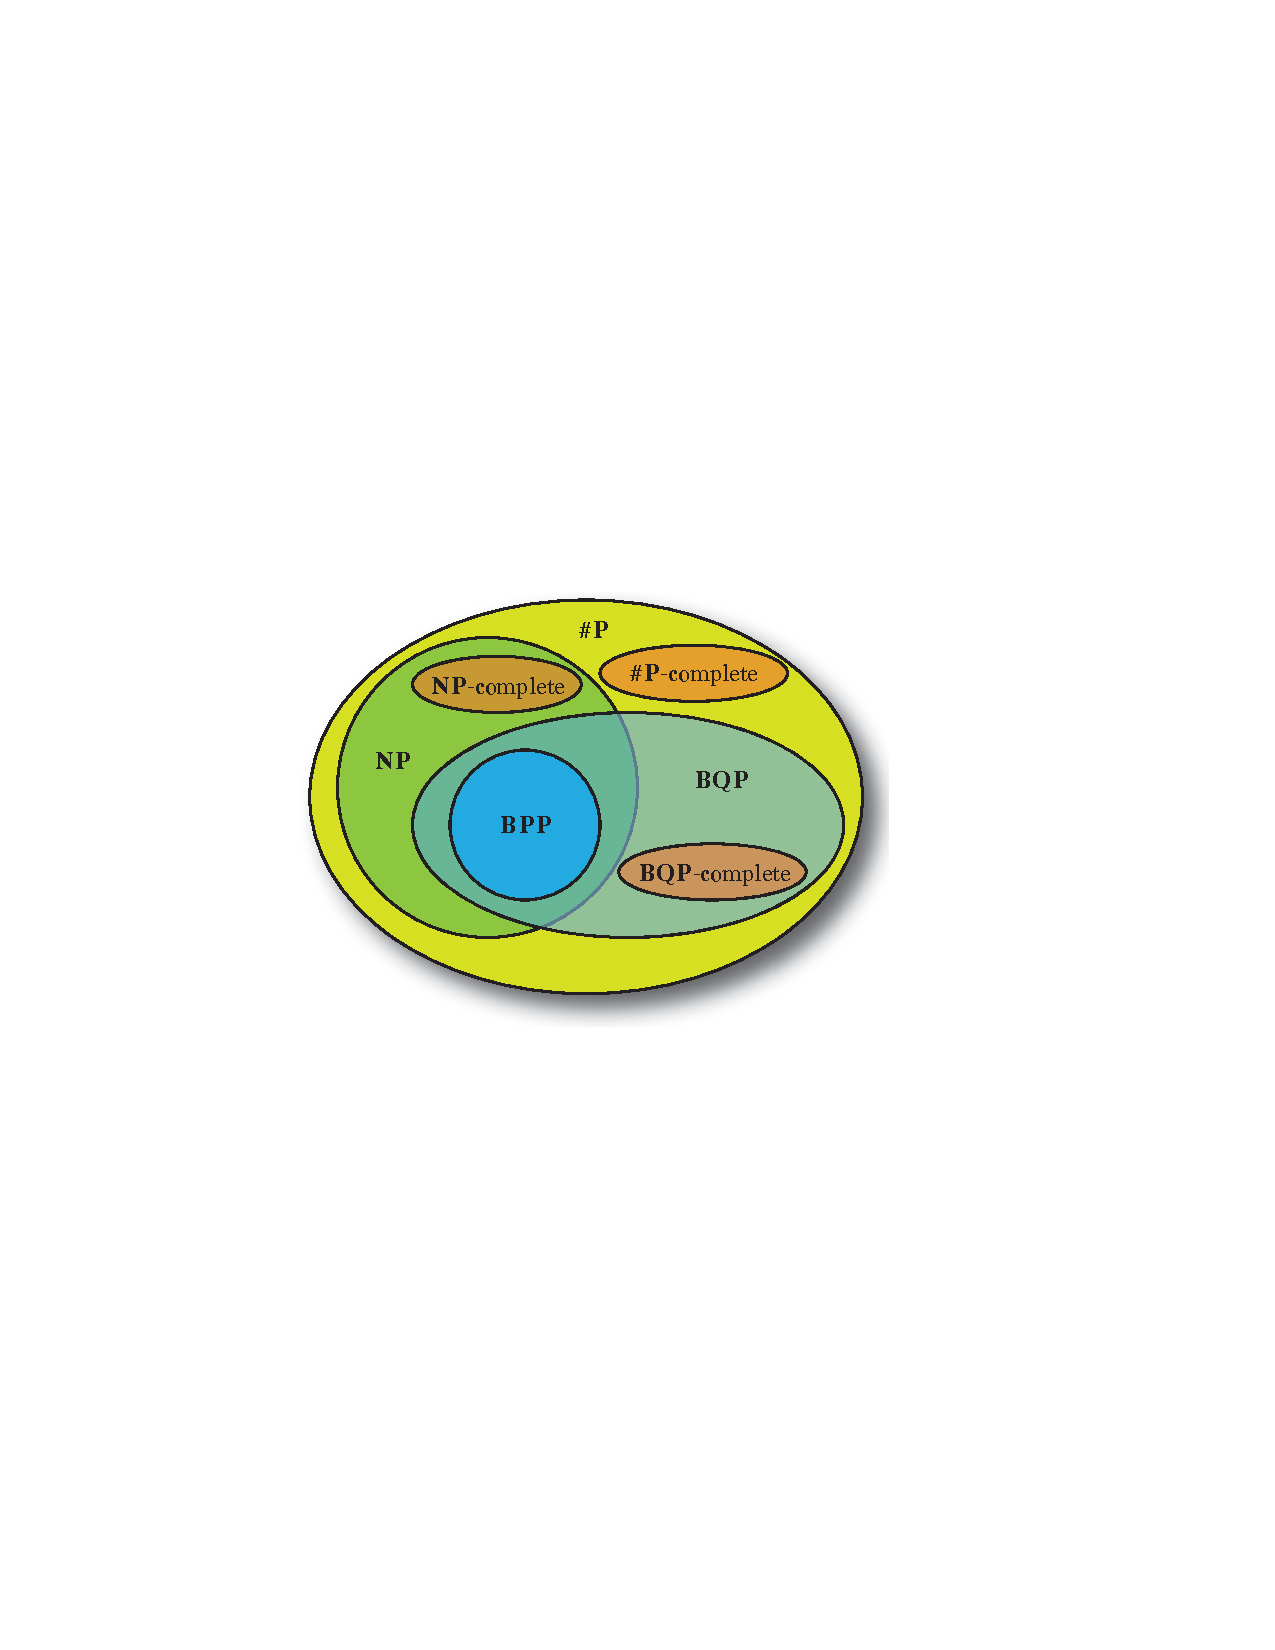
\includegraphics[width=\columnwidth]{complexity_classes}
\caption{Believed relationships between the complexity classes most relevant to quantum computing. \textbf{BPP} is the class of polynomial-time probabilistic classical algorithms. \textbf{NP} is the class of problems verifiable in polynomial time using classical algorithms. \textbf{NP}-complete are the subset of \textbf{NP} problems polynomial-time reducible to any other problem in \textbf{NP}. \textbf{BQP} is the class of probabilistic algorithms solvable in polynomial time on universal quantum computers. $\#\mathbf{P}$ is the set of counting problems, that count satisfying solutions to \textbf{BPP} problems. \textbf{BPP} is regarded as the class of problems efficiently solvable on universal Turing machines (i.e classical computers), whereas \textbf{BQP} is that solvable on universal quantum computers. The computational superiority of quantum computers is based on the (strongly believed, yet unproven) assumption that \mbox{$\mathbf{BPP}\subset\mathbf{BQP}$}.} \label{fig:complexity_classes}
\end{figure}

Aside from quantum computing, quantum cryptography holds the promise of uncrackable cryptographic protocols, guaranteed not by the assumed complexity of solving certain mathematical problems like integer factorisation, but by the laws of quantum mechanics. That is, provided our understanding of quantum mechanics is correct, quantum cryptographic protocols exists which cannot be cracked, irrespective of the computational resources of an adversary.

Already we are beginning to see elementary realisations of essential quantum technologies such as quantum computing, cryptography, and metrology. As these technologies become increasingly viable and more ubiquitous, the demand for networking them and sharing quantum resources between them will become a pressing issue. Most notably, quantum cryptography and \emph{cloud quantum computing} will be pivotal in the proliferation of quantum technology, which necessarily requires reliable quantum communications channels.

The first demonstrations of digital computer networks were nothing more than simple two-party, point-to-point communication. However, the internet we have today extends far beyond this, allowing essentially arbitrary worldwide networking across completely ad hoc networks comprising many different mediums, with any number of parties, in an entirely plug-and-play fashion. Similarly, elementary demonstrations of quantum communication have been performed across a small number of parties, and much work has been done on analysing quantum channel capacities in this context \cite{??? channel_capacity}. But, as with digital computing, demand for a future \emph{quantum internet} is foreseeable, enabling the arbitrary communication of quantum resources, between any number of parties, over ad hoc networks.

The digital internet may be considered a technology stack, such as TCP/IP (Transmission Control Protocol/Internet Protocol), comprising different levels of abstraction of digital information \cite{bib:TanenbaumNet}. At the lowest level we have raw digital data we wish to communicate across a physical medium. Above this, we decompose the data into packets. The packets are transmitted over a network, and TCP is responsible for routing the packets to their destination, and guaranteeing data integrity and Quality of Service ({\sc QoS}). Finally, the packets received by the recipient are combined and the raw data reconstructed.

The TCP layer remains largely transparent to the end-user, enabling virtual software interfaces to remote digital assets that behave as though they were local. This allows high-level services such as the File Transfer Protocol (FTP), the worldwide web, video and audio streaming, and outsourced computation on supercomputers, as though everything was taking place locally, with the end-user oblivious to the underlying networking protocols. To the user, YouTube videos or Spotify tracks behave as though they were held as local copies. And FTP allows storage on a data centre to be mounted as though it were a local volume. We foresee a demand for these same criteria in the quantum era.

In the context of a quantum internet, packets of data will instead be quantum states, and the transmission control protocol is responsible for guiding them to their destination and ensuring quality control.

Here we present a treatment for such Quantum Transmission Control Protocols (QTCP's) as a theoretical foundation for a future quantum internet. We consider how such ad hoc networks may be described mathematically, how to quantify network performance, and present a QTCP stack for operating it. While the goals of QTCP are similar as for classical TCP, there are major conceptual differences between the classical and quantum internets, owing to the unique properties of quantum states with no classical analogue.

Our treatment of quantum networks will be optics-heavy, based on the reasonable assumption that communications channels will almost certainly be optical, albeit with many possible choices of optical states and mediums. However, this does not preclude non-optical systems from representing quantum information that is not in transit, and we consider such `hybrid' architectures in detail, as well as the interfacing between optical and non-optical systems. Indeed, it is almost certain that future large-scale quantum computers will not be all-optical, necessitating interfacing different physical architectures. We accommodate for this requirement in the design of the QTCP.

The quantum internet will enable advances in the large-scale deployment of quantum technologies. Most notably, in the context of quantum computing it will allow initially very expensive technology to be economically viable and broadly accessible via the outsourcing of computations from consumers who can't afford quantum computers, to well-resourced hosts who can -- \emph{cloud quantum computing}.

With the addition of recent advances in homomorphic encryption and blind quantum computing, such cloud quantum computing can be performed securely, guaranteeing privacy of both data and algorithms, secure even against the host performing the computation. This opens up entirely new economic models and applications for the licensing of compute time on future quantum computers in the cloud.

But quantum technologies extend far beyond computation. Many other exciting applications for controlled quantum systems exist, with new ones frequently emerging. Thus, the quantum internet will find utility beyond cloud quantum computing, enabling the global exchange of quantum resources and assets. This could include the networking of elementary quantum resources such as state preparation, entanglement sharing, teleportation and quantum measurements, or scale all the way up to massively distributed quantum computation or a global quantum cryptography network.

It is hard to foresee the future of quantum technology, much as no one foresaw the advances digital technology has made over the last half century. But it is certain that as the internet transformed digital technology, the quantum internet will define the future of quantum technologies.

%
% Classical Networking Protocols
%

\section{Classical networking protocols} \label{sec:classical_nets}

To set the context for our upcoming treatment of quantum networks, we begin by discussing \emph{classical} networks, and some of the key protocols behind their operation.

There have been numerous approaches employed in the past for sharing communications links between multiple users. This includes channel-switched networks, time- or frequency-multiplexed networks, and Code Division Multiple Access (CDMA). Nowadays packet-switched networks have become the norm in most digital networks, as they facilitate far greater efficiency in the use of network bandwidth, and are more easily scaled to greater numbers of users in a dynamic and ad hoc manner. It is foreseeable the same trend will continue with quantum technologies, especially given their initial high cost, where maximising network utility is paramount.

In this work we will focus on packet-switched networks when we later introduce our quantum networking protocols. However, with sufficient flexibility in the design of our upcoming quantum protocols, packet-switched networks can easily be made to effectively implement channel-switched, or time-/frequency-multiplexed communication.

The present-day internet is built on top of a protocol stack comprising primarily the Internet Protocol (IP), User Datagram Protocol (UDP), and Transmission Control Protocol (TCP). Most commonly, these are simply referred to as TCP/IP. These define a protocol stack of different layers of abstraction for communicating data packets between nodes in a network, determining their routing, and enforcing any quality of service requirements.

%
% Internet Protocol (IP)
%

\subsection{Internet Protocol (IP)}

IP is the standard protocol employed in the internet for communicating data packets point-to-point. It is a low-level protocol that encapsulates digital data into packets containing a header field, which specifies routing information, most notably the IP addresses of the source and destination. IP does not enforce any kind of quality control, which is instead delegated higher-level protocols like TCP (Sec.~\ref{sec:TCP}, a higher-level protocol built on top of IP (Sec.~\ref{sec:TCP}).

Multiple packets with the same source and destination needn't follow the same route -- the routing is determined dynamically in realtime by routers, based on network characteristics such as load or latency. Thus, packets belonging to the same underlying data may arrive out of order, or some may go missing altogether. IP does not address these issues, instead engaging in only `best-effort' delivery. 

In IP there is no central authority with knowledge of the state of the entire network, which tells routers in the network how to best route packets. Thus, IP must be complemented with up-to-date routing tables, held by routers/nodes in the network, which make routing decisions on a per-packet basis. This is achieved using gateway protocols, discussed next.

%
% Routing Tables
%

\subsection{Gateway protocols \& routing tables} \label{sec:gateway}

In the absence of a central mediating authority, routing decisions must be made by individual nodes in the network, upon receipt of packets. For routers to make sensible routing decisions, they must have some idea of overall structure and state of the network. This is achieved using gateway protocols, which communicate information about the state of the network on a nearest-neighbour basis. The are various gateway protocols in use, with the Exterior Gateway Protocol (EGP) and Border Gateway Protocol (BGP) being very common.

We let every node in the network have a routing table, initially empty, that will ultimately be populated with information on how to best route incoming packets further along the route to their destination.

To mitigate the need for a central authority, nodes engage in only nearest neighbour communication, sharing their routing tables with one another, to query about the distance metrics (Sec.~\ref{sec:costs}) associated with routes to different destinations. This communication is taking place regularly, and as nodes' routing tables become populated, updating in real-time, they will (hopefully) reach a steady-state. From these tables, single-source shortest path algorithms (Sec.~\ref{sec:single_source_sp}) can be applied by nodes to construct a complete picture of costs to every point in the network.

%
% User Datagram Protocol (UDP)
%

\subsection{User Datagram Protocol (UDP)}

The UDP is a simple protocol built on top of IP, based on a `send-and-forget' principle for sending data packets. That is, there is no quality of service guarantee, and no notifications are provided to the sender as to whether packets successfully reached their destination. However, a checksum (hash) forms a part of the packet headers to enable error detection by the recipient. The lack of quality control bypasses the associated latency, making it particularly useful in time-critical applications, where the late arrival of a packet is useless and therefore needn't be retransmitted.

UDP is connectionless, meaning that no designated connection is established between hosts. Instead data is simply transmitted and then forgotten about. The receiver may not even be operational on the network, in which case the packets are lost without notice.

Key examples for the use of UDP are realtime audio and video transmission. If a packet associated with a frame in a video link is delayed, it is useless, since it is associated strictly with a particular frame in the video. Quality control therefore would achieve nothing. This applies similarly to live audio streaming, such as voice-over-IP (VoIP), where the late arrival of a packet cannot possibly be correctly inserted into the audio playback and might as well be discarded.

Therefore, UDP prioritises latency over reliability, and is best suited to time-critical applications where quality of service is not relevant.

%
% Transmission Control Protocol (TCP)
%

\subsection{Transmission Control Protocol (TCP)} \label{sec:TCP}

TCP differs from UDP in that it intrinsically supports quality control. The protocol is able to determine whether a packet successfully reached its destination, and if not, retransmit it as often as necessary to guarantee packet delivery. A checksum is also included in packets to enable error detection. This quality control has made TCP the dominant protocol employed in the present-day internet, where, in most scenarios, we wish to guarantee that data has been correctly delivered -- if an email is missing random segments of its text, users will become irate very quickly!

TCP is connection-oriented, meaning that a handshaking protocol establishes a dedicated bidirectional channel between two hosts. It also enforces packet reordering, to counter out-of-order packet arrival.

However, the enforced quality control and handshaking protocols incur a network performance overhead that UDP does not, since handshaking protocols consume bandwidth. Thus, TCP should not be used instead of UDP if there are no quality of service requirements.

%
% Ethernet
%

\subsection{Ethernet}

Ethernet is a networking protocol based on `broadcasting' on a shared network. This model is particularly suited to local area networks (LAN's), where all users share a single communications channel rather than dedicated point-to-point links.

In the Ethernet protocol, every user is free to broadcast data onto the shared channel as they please -- all users transmit to, and receive from a single shared channel. However, clearly sometimes packet `collisions' will occur, resulting in packet corruption. To overcome this, Ethernet packets contain a checksum that can be used to verify upon arrival whether a packet has been corrupted by a collision. If a collision is detected, the respective users are able to re-broadcast, following a randomly chosen waiting period (known as `backoff'). Collisions therefore reduce network performance, and it follows that network bandwidth decreases with the number of users competing for bandwidth\footnote{Think of that awkward dinner table conversation, where two people start talking simultaneously. It's immediately obvious to them both that they are interfering with one another, and if they were to just talk over one another (packet collision), no one would understand either of them. So, they both awkwardly pause, before starting to speak again. In a \emph{really} awkward conversation, they will both start again simultaneously, after which there will be an even longer awkward pause before recommencing. Eventually, this self-regulating system will resolve itself probabilistically, with a sole victor controlling the airwaves, commanding the attention of the listeners. Provided that all dinner guests adhere to social etiquette and backoff appropriately, with repeated conversations, all guests will statistically receive an equitable share of attention, albeit with some wastage of conversation time owing to the periods of silence. Clearly, the proportion of the time wasted due to collisions will scale up with the number of guests, limiting the protocol to not-too-large tables.}.

From this protocol, any given packet will eventually be successfully transmitted uncorrupted, collision-free, albeit with uncertain timing that grows with the number of competing users. For this reason, the Ethernet protocol is not ideal for time-critical applications requiring hard guarantees on network latency.

The beauty of this approach is that only a single channel is required for connecting all users. No dedicated point-to-point connections are required. As the number of users increases, the complexity of the network topology does not -- requiring only the addition of a node to the existing backbone. For small LAN's this is clearly reasonably functional. However, as the size of networks increases, the rate at which packet collisions occur increases, resulting in a reduction in network bandwidth. Thus, the Ethernet protocol is ideally suited to small LAN's, but is clearly not viable at a global level, where network competition is astronomical and the overhead from backoff would reduce network performance to a standstill, wasting most of the bandwidth.

Another elegant feature of the Ethernet protocol is that bandwidth allocation is self-regulating, with bandwidth fairly and equitably allocated between users. This applies even in completely ad hoc networks, with users joining and leaving the network willy nilly. Provided all users are correctly and honestly implementing the `broadcast-and-backoff' protocol, network bandwidth is allocated evenly amongst users, and no mediating, overriding central authority is needed to oversee network resource allocation. This allows Ethernet networks to be truly `plug-and-play'.

%
% Network Hierarchies
%

\subsection{Network hierarchies}

The disadvantage of Ethernet's broadcast-and-backoff principle is that packets are often wasted -- whenever a collision occurs. Because there is no mediating central authority, packet collisions are a certainty in a heavily-utilised network, each time resulting in packet loss, and an associated reduction in usable network bandwidth.

To the other extreme, we could have dedicated point-to-point channels between every pair of users. Then there would be guaranteed no packet collisions, and therefore maximum bandwidth efficiency, but the network would be extremely costly.

To address this dilemma, the topology and subdivision of networks need to be carefully designed. If we consider a large organisation, for example, potentially networking thousands of desktop PC's, the bandwidth wastage associated with packet collisions could grind the entire network to a halt, were all thousands of PC's to be communicating large amounts of data simultaneously. However, if a hierarchy of subnetworks could be implemented, rather than a single monolithic network, efficiency could be improved drastically.

Suppose our hypothetical organisation had several different departments, and users had a tendency to communicate primarily with others users in the same department. By defining distinct departmental subnets, which individually implement Ethernet, but interconnect with one another using an alternate routing framework, we can easily see that many unnecessary packet collisions may be entirely avoided. That is, why broadcast data to users who we know don't want it?

Extending upon this simple intuitive example, enormous amounts of research and development have been invested into the design of network hierarchies, and how to optimise their efficiency.

\comment{To do}

%
% Mathematical Representation of Networks
%

\section{Mathematical representation of networks}

We now turn our attention to defining a mathematical construction for the representation of (quantum \emph{and/or} classical) networks, that we will subsequently rely on heavily in our framework for quantum networks. This encompasses representing networks as graphs, representing the cost of communications within the network, and how to optimise network routing to minimise costs.  These notions will be essential in our treatment of quantum networks.

%
% Graph-Theoretic Representation
%

\subsection{Graph-theoretic representation}

We consider a classical network to be a weighted, directed graph \mbox{$G=(V,E)$}, where vertices represent \emph{nodes} (\mbox{$v\in V$}) in the network, and the weighted edges represent communication \emph{links} (\mbox{$e\in E$}) between neighbouring nodes \cite{???}.

A node could be, for example, data storage, a classical computer implementing a computation, a router that switches the connections between incoming and outgoing links, or an end-user. A link on the other hand is any arbitrary means of communication between nodes, such as optical fibre, satellite, radio, electrical, smoke signals, tin cans connected by a taut piece of string, or well-trained carrier pigeon. In the protocols to be described here, it is completely irrelevant what the specific mediums for communication are. Rather what matters are \emph{costs}, quantifying the relative performance of different links.

A key feature of the global internet is redundancy. In a packet-switched environment, sending identical packets twice might each follow entirely different routes to their common destination. Node-to-node redundancy is easily accommodated for in the graph-theoretic model by allowing multiple distinct edges between nodes. It is extremely important to accommodate multiple edges in network graphs, since redundant routes provide a direct means by which to load-balance a route. So, for example, a hub in Australia might connect to a sister hub in New Zealand using both a fibre-optic undersea cable, and simultaneously via a satellite uplink. If the faster of the two connections is running out of capacity, a proportion of the packets can simply be switched to the other link, thereby balancing the load. For this reason we abstain from using an adjacency matrix representation for network graphs, as they do not accommodate redundancy.

%
% Network Costs & Attributes
%

\subsection{Network costs \& attributes} \label{sec:costs}

The edge weights in $G$ represent the \emph{costs} ($\vec c$) and \emph{attributes} ($\vec a$) associated with using that link. In general these needn't be single numbers, but would rather be sets, representing different types of costs and attributes of links, of which there may be many. These could include, for example, latency, bandwidth, dollar cost, and quality.

The distinction between costs and attributes, is that costs may be expressed in terms of units which may be interpreted as distances metrics in a Euclidean sense, obeying the following requirements:

\begin{definition}[Network cost metrics] \label{def:metric} Cost metrics satisfy the properties:
\begin{itemize}
    \item Identity operations: If a channel performs nothing, its associated cost is zero, \mbox{$c(\mathbb{\hat{I}}) = 0$}.
    \item Triangle inequality: $c(v_1\to v_2\to v_3) \leq c(v_1\to v_2) + c(v_2\to v_3)$, across all paths \mbox{$v_1 \to v_2 \to v_3$}.
    \item Positivity: \mbox{$c\geq 0$}. This ensures that shortest-path algorithms will function correctly.
\end{itemize}
\end{definition}
Attributes, on the other hand do not have a distance interpretation, and may have arbitrary structure. A detailed discussion on the relationship between costs and attributes is presented in Sec.~\ref{sec:c_vs_a}.

The reason we demand costs have a distance interpretation is so that graph-theoretic pathfinding algorithms (Sec.~\ref{sec:shortest_path}) are applicable, allowing us to build upon the vast pre-existing understanding of graph theory. Ideally we would like equality in costs' triangle inequality, which yields an exact cost. But often this isn't possible and we are satisfied with the inequality, which simply dictates an upper bound on cost.

A \emph{route} between two nodes, Alice ($A$) and Bob ($B$), of the network, $G$, is an acyclic subgraph connecting those nodes, \mbox{$R_{A\to B}\subset G$}. In general ad hoc networks there will typically be multiple paths between two nodes \mbox{$A\to B$}. For a particular cost metric, the cost of an entire route is simply the sum of the costs of each of the constituent links,
\begin{align}
c(R_{A\to B}) = \sum_{i=1}^{|R_{A\to B}|-1} c(v_i \to v_{i+1}),
\end{align}
where $v_i$ is the $i$th node in the route $R_{A\to B}$.

Fig.~\ref{fig:example_routes} illustrates a simple example network with all of its available routes, \mbox{$R_{A\to B} \subseteq G$}. Fig.~\ref{fig:simp_route_opt} illustrates the optimal path for \mbox{$A\to B$} based on edge weights.

\begin{figure}[!htb]
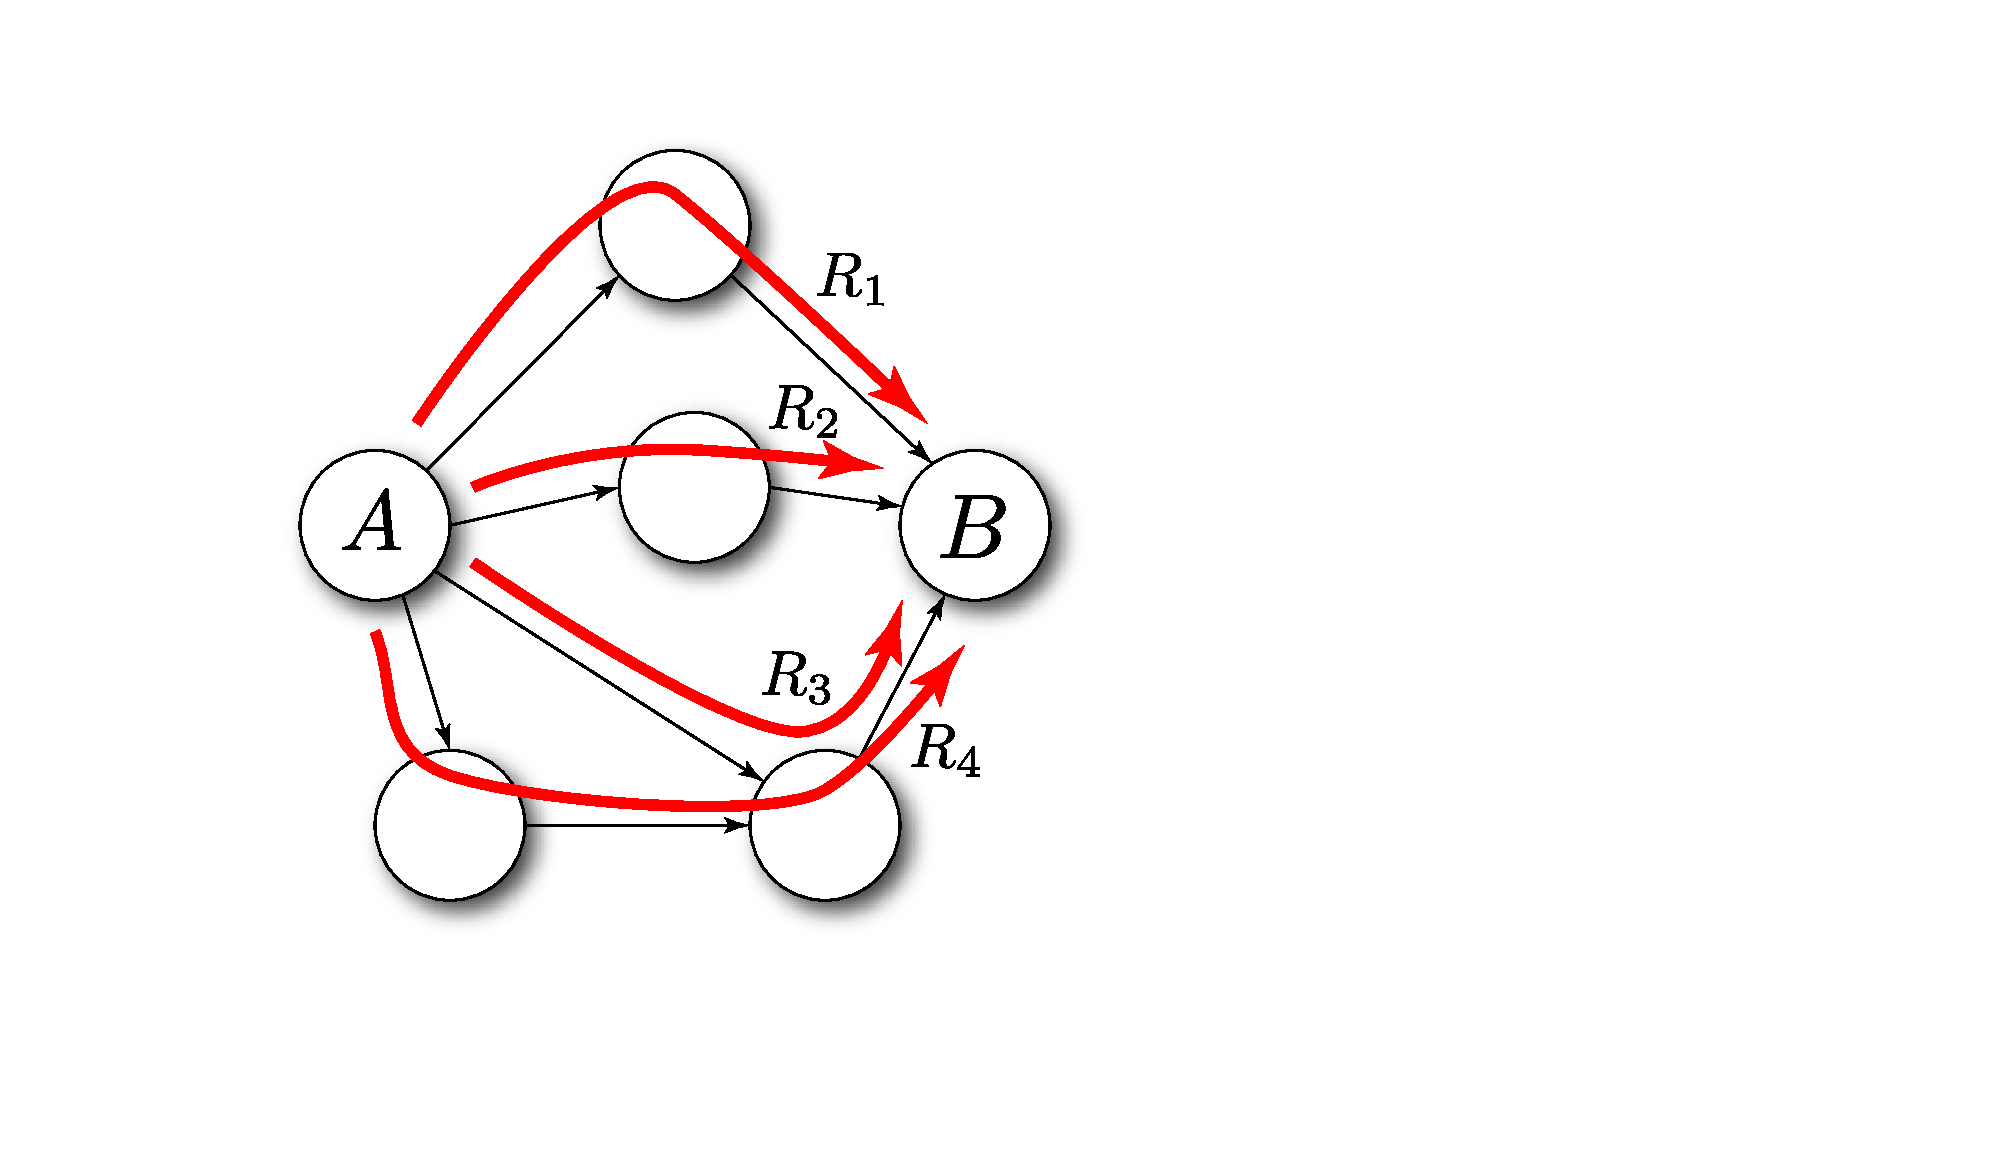
\includegraphics[width=0.65\columnwidth]{example_routes}
\caption{Example of a simple network with multiple routes \mbox{$A\to B$}. Note that $R_3$ and $R_4$ are competing with one another for use of the last link, which the routing strategy, $\mathcal{S}$, will need to resolve if multiple simultaneous transmissions are taking place.} \label{fig:example_routes}
\end{figure}

\begin{figure}[!htb]
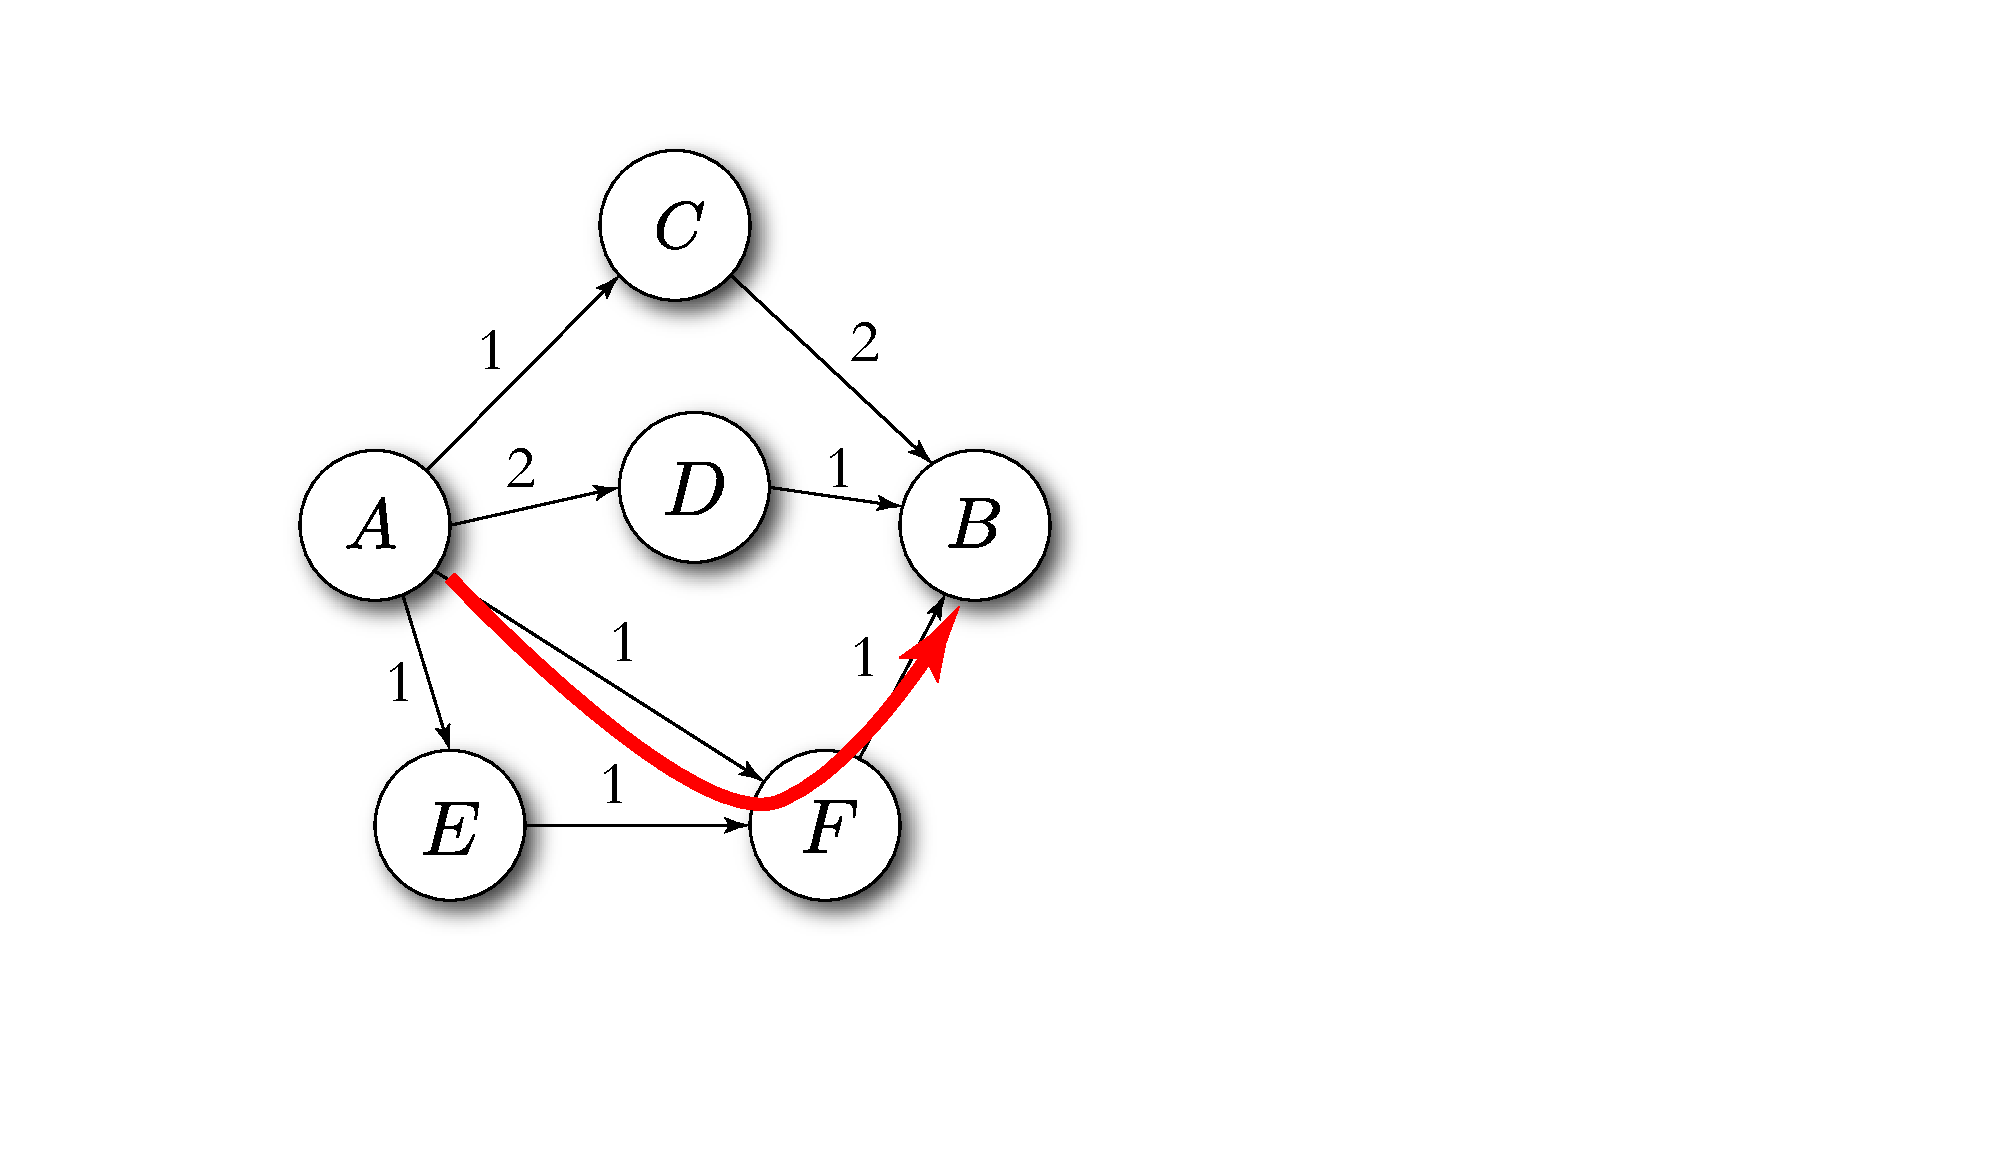
\includegraphics[width=0.6\columnwidth]{example_opt}
\caption{The same network graph from Fig.~\ref{fig:example_routes}, with links weighted by some arbitrary cost metric. Applying a shortest-path algorithm yields the optimal route between Alice and Bob to be \mbox{$A\to F\to B$}, which incurs a net cost of \mbox{$c=2$}, as opposed to all other routes, which incur a net cost of \mbox{$c=3$}.} \label{fig:simp_route_opt}
\end{figure}

In a given network, it is unlikely that only a single cost metric or attribute will be of interest when determining optimal routings. There may be a tradeoff between different measures. For example, for time-critical applications the cost of a route might be considered a combination of both dollar cost and latency -- a satellite has very low latency but is extremely expensive, while a carrier pigeon is slow but cheap (and prohibited by PETA). What is the best tradeoff between the two?

To accommodate this, we allow the \emph{net cost} of a route to be defined as an arbitrary function of other primitive cost metrics and attributes of the route,
\begin{align} \label{eq:net_cost_R}
c_\mathrm{net}(R) = f_\mathrm{cost}(\vec{c}(R),\vec{a}(R)),
\end{align}
where $c_\mathrm{net}$ is a single numeric value representing the net cost as calculated from an arbitrary cost function $f_\mathrm{cost}$. Note that the net cost needn't be a metric, as the cost function could be arbitrary. The net cost can be thought of as a ranking for routes, but not necessarily as a metric that accumulates across routes.

Eq.~\ref{eq:net_cost_R} gives us the net cost of a given route. For multiple users we would like to simultaneously optimise the cost across all users of the network. Thus we define the routing cost for the entire network to be,
\begin{align} \label{eq:c_total}
c_\mathrm{total}(\vec{R}_{\vec{A}\to \vec{B}}) = \sum_{r \in {\vec R}_{\vec{A}\to \vec{B}}} c_\mathrm{net}(r),
\end{align}
where $\vec{R}_{\vec{A}\to \vec{B}}$ is a set of routes connecting each pair \mbox{$A_i\to B_i~\forall ~ i$}.

%
% Flow Networks
%

\subsection{Flow networks} \label{sec:flow_networks}

On a shared network with many users utilising the network simultaneously, it may be the case the preferred goal for the network is to maximise \emph{flow} \cite{???} -- the total amount of information that can be transmitted per unit time, i.e the net utilisation of the network's resources, summed over all users. In this case we can build on the existing theory of \emph{flow networks} \cite{???}, which characterise the load of links within the network.

A flow network is easily obtained from the network graph by associating a `capacity' attribute with each link and defining the graph weighted by the capacities as the flow network, preserving the underlying structure of the network graph.

When a route within the graph is utilised, we decrement the capacities of each link in that route, generating the so-called \emph{residual network} \cite{???}, which will now take the place of the original network in subsequent calculations. This process effectively tallies the links' utilisation, and when the tally hits zero, the link can no longer be used for any new routes. This forms a basic building block for more complex flow network algorithms.

There are many variations on flow networks. The simplest case is of a single user transmitting multiple packets simultaneously to a recipient. Depending on link capacities, different packets may need to follow different routes through the network, if network performance is to be maximised. Alternately, it may not be possible to send the desired number packets simultaneously if the network capacity saturates.

The more complex (and realistic) scenario is of multiple users each transmitting from distinct starting nodes to distinct recipient nodes across a shared network. This is known as a \emph{multi-commodity flow network} \cite{???}, and is likely to be the dominant class of networks in real-world networking applications.

%
% Routing Strategies
%

\subsection{Routing strategies} \label{sec:route_strats}

A \emph{strategy}, $\mathcal{S}$, is simply an algorithm that chooses a route ($k$), based on the starting ($i$) and finishing ($j$) nodes of a communication, and also updates the vectors of costs and attributes within the network associated with the utilisation of that route,
\begin{align}
\mathcal{S}(i,j,\vec{c},\vec{a}) &\to \{k,{\vec{c}}~',{\vec{a}}~'\}, \nonumber \\
i,j &\in V, \nonumber\\
k &\in \{R_{v_i\to v_j}\},
\end{align}
with the goal of minimising a chosen cost measure.

No particular route through a network is going to have infinite capacity, and therefore we cannot typically always reemploy the same most cost-effective route for all data. Particularly in multi-user networks, as routes are employed for communicating quantum states, their cost metrics may change according to load, or other external influences. For this reason, it is important that strategies accommodate dynamic changes in the network. This is easily accounted for by letting the edge weights in our network graph be a function of time, $G_t$, which are updated via the application of a strategy, which may also be a function of time,
\begin{align} \label{eq:S_G}
G_{t+1} = \mathcal{S}_t(G_t).
\end{align}
For example, the network might have bandwidth restrictions on some links, in which case if more than a certain amount of data is transmitted through a link, it is no longer available for use until previous transmissions have completed. Or, based on market dynamics, the dollar cost of utilising a link may change with its demand.

This type of cost minimisation approach to routing is analogous to \emph{distance-vector routing protocols} in classical networking theory.

%
% Strategy Optimisation
%

\subsection{Strategy optimisation} \label{sec:strat_opt}

Clearly the goal when choosing routing strategies is to minimise the total cost, Eq.~\ref{eq:net_cost_R}. That is, solving the optimisation problem,
\begin{align}
c_\mathrm{min} &= \min_\mathcal{S} (c_\mathrm{total}), \nonumber \\
\mathcal{S}_\mathrm{opt} &= \mathrm{argmin}_\mathcal{S} (c_\mathrm{total}).
\end{align}

Choosing optimal strategies is a challenging problem, potentially requiring complex, computationally inefficient optimisation techniques. Strategy optimisation is an example of resource allocation, whose optimal solutions are often notoriously difficult to solve, residing in complexity classes like \textbf{NP}-complete (or worse!). In general, the number of possible routes through a graph will grow exponentially with the number of vertices. Thus, explicitly enumerating each possible route is generally prohibitive for large networks, unless some known structure provides `shortcuts' to optimisation. Having said this, Dijkstra's shortest path algorithm (discussed in Sec.~\ref{sec:shortest_path}) is the perfect counterexample, demonstrating that although an exponential number of routes may exist between two points, an optimal one can be found in polynomial time.

%
% Ad hoc Operation vs. Central Authorities
%

\subsubsection{Ad hoc operation vs. central authorities}

When considering strategy optimisation, the first question to ask is `Who performs the optimisation, and who has access to what information?'.

In terms of who performs the optimisation, the two main options are that either each node is responsible for optimising the routes of packets passing through it ({\sc Individual} algorithms), or there is a reliable and trusted central authority who oversees network operation and performs all strategy decision-making ({\sc Central} algorithms).

In the case of {\sc Individual} algorithms, the required knowledge of the state of the network could be obtained using network exploration algorithms (Sec.~\ref{sec:path_exp}) or gateway protocols (Sec.~\ref{sec:gateway}). 

On the other hand, for {\sc Central} algorithms, either network exploration could be employed, or alternately the network policy could require nodes to notify the central authority upon joining or leaving the network. The former introduces an overhead in classical networking resource usage, since network exploration must be performed routinely to keep the ledger of nodes up-to-date. The latter, on the other hand, avoids this, but introduces a point of failure, in that all network participants must be reliable in notifying the central authority as required by the network policy. Failure to do so could result in invalid strategies.

%
% Local vs. Global Optimisation
%

\subsubsection{Local vs. global optimisation}

There are two general approaches one might consider when choosing strategies -- \emph{local optimisation} ({\sc Local}) and \emph{global optimisation} ({\sc Global}). {\sc Local} simply takes each state to be communicated, one-by-one, and allows it to individually choose an optimal routing strategy based on the state of the network at that moment. {\sc Global} is far more sophisticated and simultaneously optimises the sum of the routing costs, Eq.~\ref{eq:c_total}, of all currently in-demand routes.

To implement {\sc Local} optimisation, either {\sc Individual} or {\sc Central} algorithms may be employed. On the other hand, {\sc Global} optimisation necessarily requires a {\sc Central} algorithm, since it requires knowledge of the entire state of the network, which is collectively optimised.

Since {\sc Global} represents the class of all algorithms that take all network costs by all packets into consideration, it must clearly perform at least as well as {\sc Local}, which only takes into consideration the costs of a given packet. But we expect {\sc Global} to perform better than {\sc Local} in general, owing to the additional information it takes into consideration. We express this as \mbox{{\sc Local}$\subset${\sc Global}}. However, {\sc Global} requires solving a complex, simultaneous optimisation problem, which is likely to be computationally hard, whereas {\sc Local} can be efficiently solved using multiple independent applications of, for example, an efficient shortest-path algorithm (so-called {\sc Greedy} algorithms), discussed in Sec.~\ref{sec:shortest_path}.

A further stumbling block for {\sc Global} is that it requires some central authority, responsible for the global decision-making, to have complete, real-time knowledge of the state of the entire network. This may be plausible for small Local Area Networks (LAN's), but would clearly be completely implausible for the internet as a whole. So it is to be expected that different layers and subnets in the network hierarchy will employ entirely different strategy optimisation protocols. This is certainly reminiscent of the structure of the present-day internet.

Roughly speaking, we might intuitively guess that at lower levels in the network hierarchy, responsible for smaller subnets, there will be a tendency towards the adoption of {\sc Global} strategies, as full knowledge of the state of the subnet is readily obtained. However, as we move to the highest levels of the network hierarchy (e.g routing of data across international or intercontinental boundaries), we might expect more laissez-faire (i.e {\sc Greedy}) strategies to be adopted, since the prospects of enforcing a central authority with full knowledge of the state of the internet, who is also trusted by all nations to fairly and impartially allocate network resources and mediate traffic, is highly questionable.

We will not aim to comprehensively characterise the computational complexity of {\sc Global} strategies. However, in Sec.~\ref{sec:strategies} we will present some elementary analyses of several toy models for realistic strategies. Some such strategies are efficient although not optimal, but nonetheless satisfy certain criteria we might expect.

Future developments in the optimisation techniques required for {\sc Global} strategies may improve network performance, leaving our techniques qualitatively unchanged.

When employing {\sc Local}, on the other hand, things are often far simpler. If we are optimising over a cost metric satisfying the distance interpretation, we may simply employ a shortest-path algorithm to find optimal routes through the network.

If one were to become even more sophisticated, one might even envisage treating network resource allocation in a game theoretic context \cite{???}, which we won't even begin to delve into here.

%
% Message- vs. Packet-Level Routing
%

\subsection{Message- vs. packet-level routing}

In Eq.~\ref{eq:S_G} we defined the action of a strategy, $\mathcal{S}$, on a network, $G$. However, we were intentionally ambiguous in our introduction of the time-dependence, given by $t$. This is to allow us to consider changes at one of two different time-scales: the packet level, or the message level. The \emph{message} is the entire data stream transmitted from Alice to Bob, whereas the \emph{packet} is a small block of data taken from the message, where each packet may be independently routed.

When defining the action of strategies, we could do so at either of these time-scales. We could choose routes in their entirety, from start to finish, at the beginning of the message transmission, under the assumption that the costs in the network will be constant over that duration and no one will misbehave. We refer to such strategies as \emph{message-level strategies}. Alternately, and perhaps more realistically in many scenarios, the costs and attributes of a network could be highly dynamic and readily change within the transmission time-window. In that case, we will employ \emph{packet-level strategies}, which reevaluate the strategy independently for each packet and for each of their hops between nodes.

In our future discussions on routing strategies, context will make it clear when we are referring to packet-level or message-level strategies.

%
% Quantum Networks
%

\section{Quantum networks} \label{sec:quant_net}

Quantum networks comprise all the same ingredients as classical networks, but with additions. Nodes can additionally implement quantum computations, quantum-to-classical interfaces (i.e measurements), quantum-to-quantum interfaces, quantum memories, or any quantum process in general. The cost associated with links could include measures that are uniquely quantum, such as fidelity, purity or entanglement measures, none of which are applicable to classical digital data. As in the classical case, our goal is to find routing strategies that optimise a chosen cost measure. But in the quantum context costs will be constructed entirely differently owing to the quantum nature of the information being communicated.

We envisage a network with a set of senders, $\{A_i\}$, and receivers, $\{B_i\}$, residing on a time-dependent network graph $G_t$ as before. $A$ have sets of quantum states to communicate, $\{\hat\rho_\mathrm{data}(i)\}$. For each $\hat\rho_\mathrm{data}(i)$ she must choose appropriate strategies $S_t$, such that the overall cost is optimised, for some appropriate cost measure. Compared to classical resources, equivalent quantum resources are costly and must be used efficiently, making resource allocation strategies of utmost importance.

The routing strategies we introduce in Sec.~\ref{sec:strategies} will not always guarantee that packets have immediate access to network bandwidth the moment they demand it. Inevitably, in shared networks there will sometimes be competition and congestion, forcing some users to wait their turn. For this reason, many quantum networks will require at least some nodes (the ones liable to competition) to have access to quantum memories, such that quantum packets can be stored for a sufficient duration that they can wait their turn on the shared network resources. Of course, quantum memories induce quantum processes of their own, which need to be factored into cost calculations. Quantum memories are easily accommodated for in the QTCP framework by allowing self-loops at nodes, which implement a memory process. The implementation of quantum memory is discussed in Sec.~\ref{sec:memory}.

Given that classical networking is decades more advanced than quantum networking, and extremely cheap and reliable, we will assume that classical resources `come for free', and only quantum resources are of practical interest. That is, classical communication and computation is a free resource available to mediate the operation of the quantum network. We therefore envisage a \emph{dual network} with two complementary networks operating in parallel and in tandem -- the quantum network for communicating quantum data, and a topologically identical classical network operating side-by-side and synchronised with the quantum network.

The motivation for the dual network is to ensure that classical and quantum data that jointly represent packets (Sec.~\ref{sec:prot_stack}) remain synchronised and subject to the same QoS issues, such as packet collisions (Sec.~\ref{sec:collision}) and network congestion.

We envisage quantum networks to extend beyond just client/server quantum computation, to include the free trade of any quantum asset. This includes state preparation, measurement, computation, randomness, entanglement, and information. Much like the classical internet, by allowing quantum assets to be exchanged, we can maximise utility, improve economy of scale, and enable new models for commercialisation.

%
% Quantum Channels
%

\section{Quantum channels} \label{sec:quant_chan}

Like classical channels, quantum channels are inevitably subject to errors. These errors could be an intrinsic part of the system, or induced by interaction with the external environment. The \emph{quantum process} formalism provides an elegant mathematical description for all physically realistic error mechanisms \cite{bib:NielsenChuang00, bib:Gilchrist05}. Here we review the quantum process formalism and discuss several specific error models that will be of particular interest in quantum networks. This paves the way for the quantum notion of costs and attributes.

%
% Quantum Processes
%

\subsection{Quantum processes}

To quantify the operation of nodes and links within our network, we must characterise the evolution they impose upon quantum states passing through them. Quantum processes, also known as \emph{trace-preserving, completely positive maps} (CP-maps) are able to capture all the physical processes relevant to quantum networking, such as: unitary evolution; decoherence; measurement; quantum memory; state preparation; switching; and, indeed entire quantum computations. And they are able to capture physical processes in any degree of freedom, most commonly in the qubit basis, but also, for photons, in the spatio-temporal, photon-number, or polarisation degrees of freedom.

Quantum processes are most easily represented using \emph{Kraus operators}, $\{\hat{K}_i\}$,
\begin{align}
\mathcal{E}(\hat\rho) = \sum_i \hat{K}_i \hat\rho \hat{K}_i^\dag,
\end{align}
where,
\begin{align}
\sum_i \hat{K}_i^\dag \hat{K}_i = \hat{\mathbb{I}}.
\end{align}
Here $\mathcal{E}$ is a super-operator, denoting the action of the process on state $\hat\rho$. This representation has the elegant interpretation as the probabilistic application of each of the Kraus operators, with probability,
\begin{align}
p_i = \mathrm{tr}(\hat{K}_i \hat\rho \hat{K}_i^\dag).
\end{align}
In the ideal case, the two types of evolution of interest are unitary evolution, in which case there is only one Kraus operator, \mbox{$\hat{K}_1=\hat{U}$}, and projective measurement, where there is again only one Kraus operator, \mbox{$\hat{K}_1=\ket{m}\bra{m}$}, for measurement outcome $m$.

Mathematically, quantum processes are equivalent to a state jointly undergoing unitary evolution with an external environment that is not observed (i.e traced out),
\begin{align} \label{eq:proc_environment}
\mathcal{E}(\hat\rho_S) = \mathrm{tr}_E (\hat{U}_{S,E} [\hat\rho_S\otimes \ket{0}_E\bra{0}_E] \hat{U}^\dag_{S,E}),
\end{align}
where $S$ denotes the primary system to which the process is applied, and $E$ is an auxiliary environment system.

We will require that all our states are normalised,
\begin{align}
\mathrm{tr}(\hat\rho) = 1,
\end{align}
and that our processes are \emph{trace preserving}. That is, they preserve normalisation,
\begin{align}
\mathrm{tr}[\mathcal{E}(\hat\rho)] = 1.
\end{align}

Multiple processes may be composed using the notation,
\begin{align}
\mathcal{E}_n(\dots \mathcal{E}_2(\mathcal{E}_1(\hat\rho)))=(\mathcal{E}_n \circ \dots \circ \mathcal{E}_2\circ\mathcal{E}_1)(\hat\rho).
\end{align}
In general, processes do not commute, i.e \mbox{$\mathcal{E}_1\circ \mathcal{E}_2 \neq \mathcal{E}_2\circ \mathcal{E}_1$}. Unless unitary, quantum processes are irreversible, meaning that errors accumulate and cannot be overcome without the overhead of some form of quantum error correction (QEC) \cite{bib:Shor95, bib:CalderbankShor96, bib:NielsenChuang00}.

The only limitation faced by the quantum process formalism is that it is described over discrete-time only. To consider continuous-time evolution, master equations can be used. These represent the continuous-time evolution of a quantum state as a differential equation in time, combining a usual Hamiltonian term as well as decoherence terms,
\begin{align}
\frac{d\hat\rho}{dt} = -\frac{i}{\hbar}[\hat{H},\hat\rho] + \sum_j [2\hat{L}_j\hat\rho\hat{L}_j^\dag - \{\hat{L}_j^\dag\hat{L}_j,\hat\rho\}],
\end{align}
where $\hat{H}$ is the Hamiltonian of the isolated system undergoing coherent evolution, and $\hat{L}_j$ are the \emph{Lindblat operators}, capturing the incoherent component of the dynamics (i.e environmental couplings).

In this work we will only make use of discrete-time quantum processes, since they naturally correspond to the evolution of states between discrete points within a network -- we are typically only interested in the process undergone by a state from one end of a link to another, not the continuous-time dynamics of what takes place within them.

%
% Quantum Process Matrices
%

\subsection{Quantum process matrices}

In general, the Kraus operator representation for quantum processes is not unique -- there may be multiple choices of Kraus operators that implement identical processes. But if the representation is not unique, how do we compare different quantum processes? To address this, it is common to choose a `standard' basis for representing quantum processes, such that they may be consistently and fairly compared. This requires choosing a basis which is complete for operations on the Hilbert space acted upon by the process.

For example, for a single qubit, the Pauli operators -- $\hat\sigma_1$ (identity, $\mathbb{\hat{I}}$), $\hat\sigma_2$ (bit-flip, $\hat{X}$), $\hat\sigma_3$ (bit-phase-flip, $\hat{Y}$), and $\hat\sigma_4$ (phase-flip, $\hat{Z}$) -- are complete for single-qubit operations ($\mathbb{C}_2$). Therefore by decomposing our Kraus operators into linear combinations of these basis operators we have a standardised representation for single-qubit processes. Formally, for one qubit,
\begin{align} \label{eq:process_matrix}
\mathcal{E}(\hat\rho) = \sum_{i,j=1}^4 \chi_{i,j} \hat{\sigma}_i\hat\rho\,\hat{\sigma}_j^\dag.
\end{align}

The Hermitian matrix $\chi$ is known as the \emph{process matrix}, from which many other metrics of interest may be directly computed (some of which are discussed in Sec.~\ref{sec:quantum_meas_cost}). Process matrices share many properties and interpretations in common with density matrices. The diagonal elements can be regarded as the amplitudes associated with applying each of the four Pauli operators, while the off-diagonal elements represent the coherences between them, i.e whether the operations on the diagonal are being applied probabilistically or coherently. For the process to be trace preserving we require,
\begin{align}
\mathrm{tr}(\chi) = 1.
\end{align}

As an illustrative example of the interpretation of process matrices, in Fig.~\ref{fig:CNOT_proc_matrix} we show the process matrix for the CNOT gate, represented in the Pauli basis. The CNOT operator can be expressed in the Pauli operator basis as,
\begin{align}
\hat{U}_\mathrm{CNOT} = \frac{1}{2}(\hat{\mathbb{I}}\otimes \hat{\mathbb{I}} + \hat{\mathbb{I}} \otimes \hat{X} + \hat{Z}\otimes \hat{\mathbb{I}} - \hat{Z}\otimes \hat{X}).
\end{align}
Then, some density operator evolved under the CNOT gate is simply \mbox{$\hat{U}_\mathrm{CNOT}\hat\rho \,\hat{U}_\mathrm{CNOT}^\dag$}. Expanding this out, we obtain a new state comprising 16 terms, each representing the action of some combination of Pauli operators from the left and from the right. The amplitudes of these terms exactly correspond to the 16 non-zero elements of the process matrix in Fig.~\ref{fig:CNOT_proc_matrix}.

\begin{figure}[!htb]
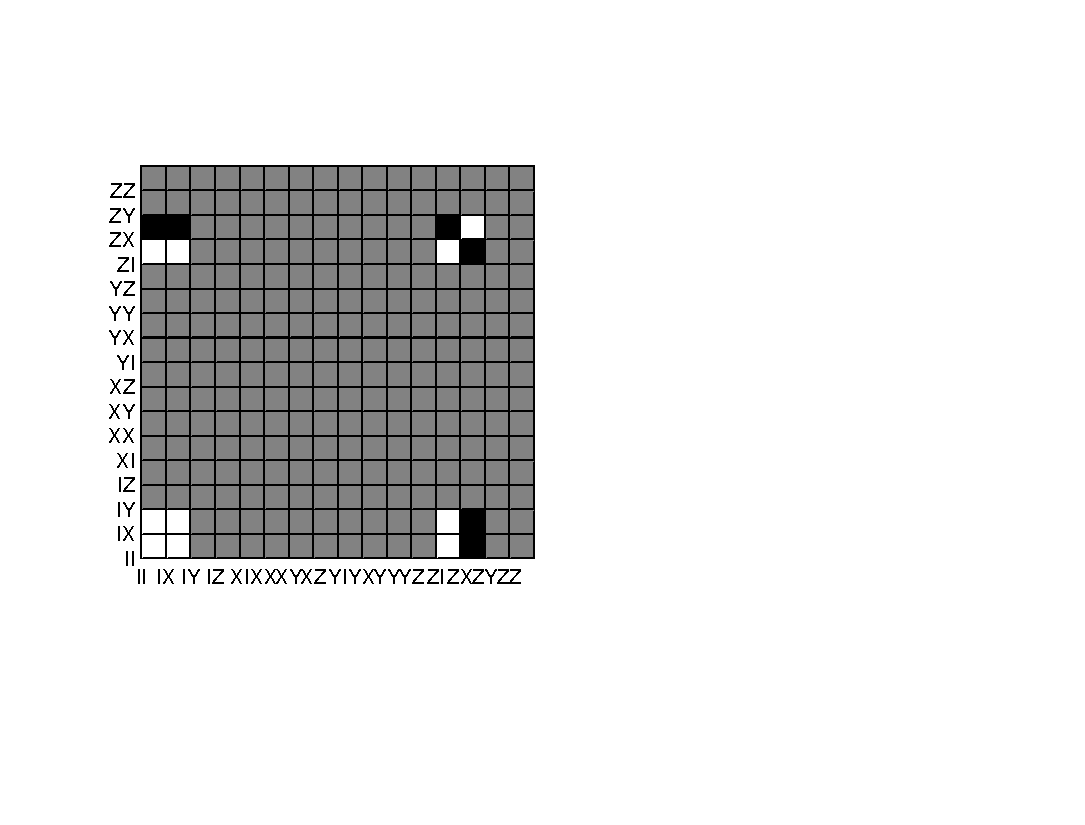
\includegraphics[width=0.7\columnwidth]{CNOT_process}
\caption{Process matrix for the CNOT gate, expressed in the Pauli basis.} \label{fig:CNOT_proc_matrix}
\end{figure}

%
% Quantum Processes in Quantum Networks
%

\subsection{Quantum processes in quantum networks} \label{sec:quant_proc_in}

Letting $v_i$ represent the $i$th node within a route $R$, the process associated with communication from that node to the next is $\mathcal{E}_{v_i\to v_{i+1}}$. For the same network used previously, Fig.~\ref{fig:example_proc_graph} shows the quantum processes associated with the links in the network. The cumulative process associated with an entire route is therefore,
\begin{align}
\mathcal{E}_R = \mathcal{E}_{{v_{|R|-1}}\to v_{|R|}} \circ \dots \circ \mathcal{E}_{v_2\to v_3} \circ \mathcal{E}_{v_1\to v_2},
\end{align}
where $|R|$ is the number of nodes in $R$, and to simplify notation, all $v_i$ are implicitly over the route $R$.

\begin{figure}[!htb]
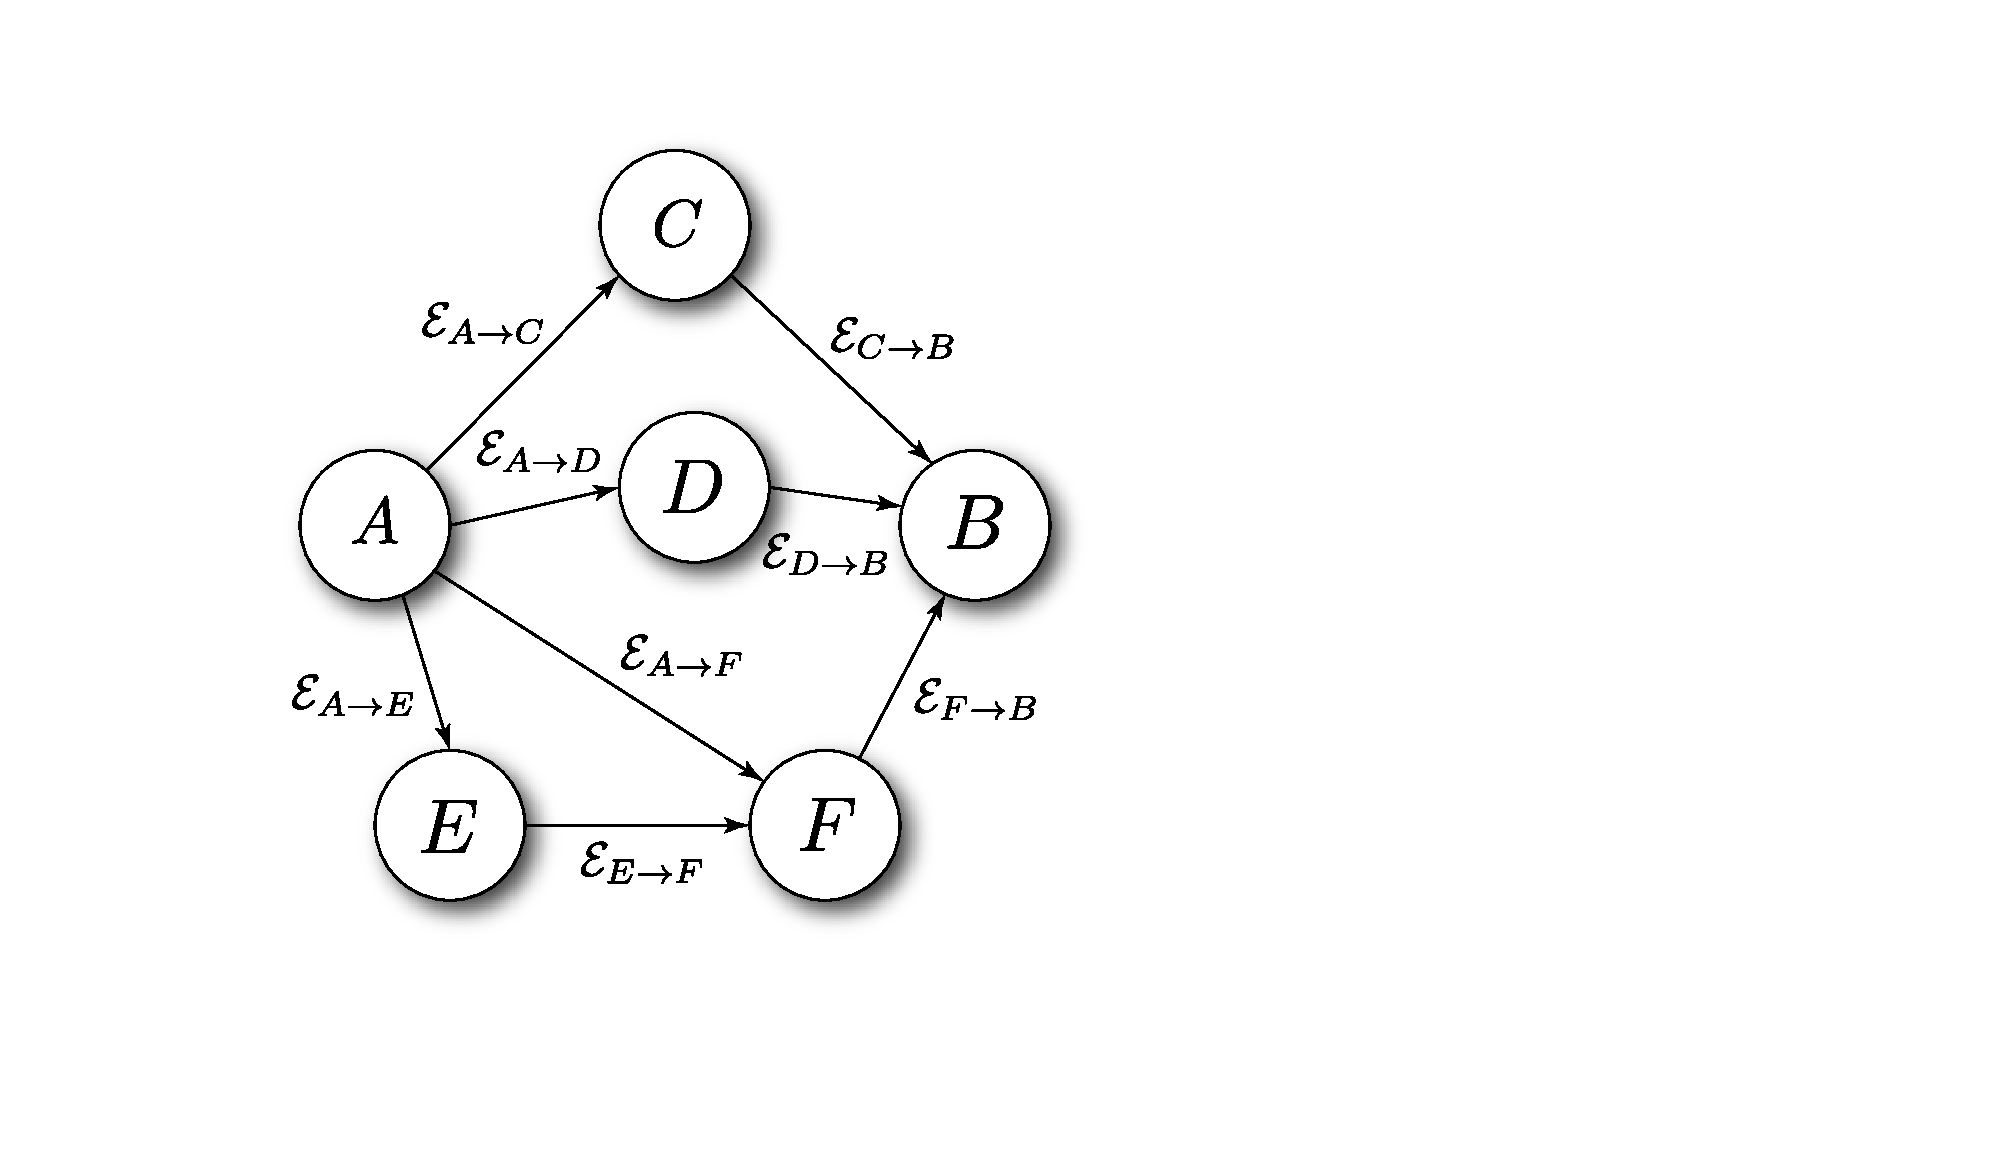
\includegraphics[width=0.6\columnwidth]{example_graph}
\caption{The network from Fig.~\ref{fig:example_routes}, with the quantum processes associated with each link. The net process associated with a route is given by the composition of each of the processes over the length of the route. For example, the route \mbox{$R_1=A\to C\to B$} induces the process \mbox{$\mathcal{E}_{R_1} = \mathcal{E}_{C\to B} \circ \mathcal{E}_{A\to C}$}.} \label{fig:example_proc_graph}
\end{figure}

In general, both nodes and links in a quantum network may implement quantum processes. However, for the purposes of compatibility with the graph-theoretic algorithms described in Sec.~\ref{sec:graph_theory}, we will eliminate node processes by merging them into link processes, such that the processes in the network are described entirely by links. This reduction procedure is straightforward, shown in Fig.~\ref{fig:remove_nodes}.

\begin{figure}[!htb]
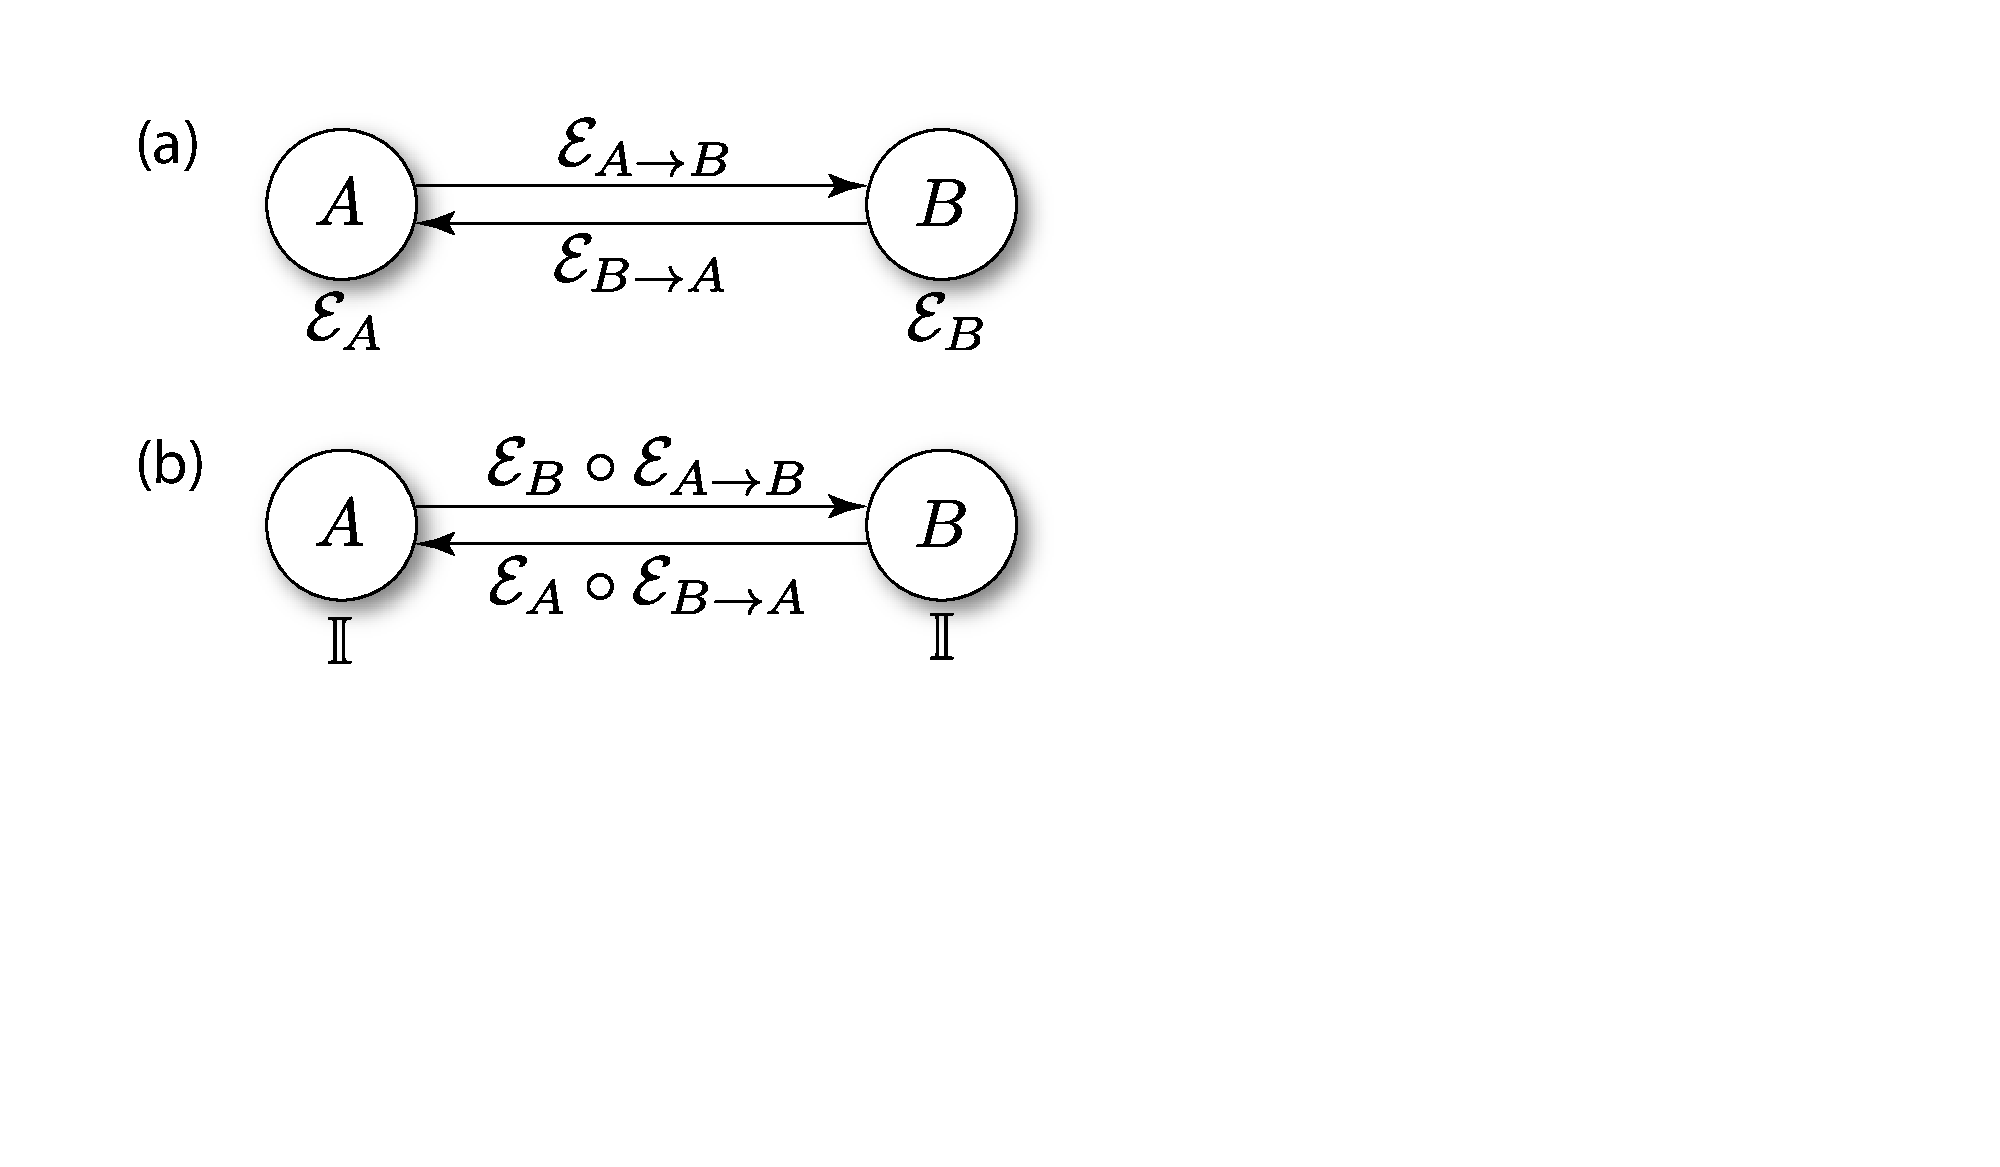
\includegraphics[width=0.7\columnwidth]{remove_nodes}
\caption{Removing node processes from network graphs on a trivial network with two nodes, $A$ and $B$. Each node is associated with a quantum process ($\mathcal{E}_A$ and $\mathcal{E}_B$). Similarly, each link is associated with a process ($\mathcal{E}_{A\to B}$ and $\mathcal{E}_{B\to A}$). (a) Representation where the node and link processes are shown explicitly. (b) The node processes are replaced with identity operations by replacing each link process with the composition of the link process and its target node process. Equivalently, the cost of each node process is added to the cost of \emph{every} incoming link and then eliminated. The same may be applied for attributes rather than costs. This procedure requires that all links be directed. If undirected links are present, they may simply be replaced by two directed links, one in each direction, implementing identical quantum processes each way.} \label{fig:remove_nodes}
\end{figure}

%
% Characterising Quantum Channels
%

\subsection{Characterising quantum channels} \label{sec:QPT}

Given a link implementing some arbitrary quantum process, it is essential that it can be experimentally determined such that network performance may be characterised. For example, if an optical channel is lossy, what is the loss rate? This is crucial when attempting to choose routing strategies that optimise certain cost metrics.

Treating a link or node as an unknown black box, \emph{quantum process tomography} (QPT) \cite{bib:ChuangNielsen97, ???} is a technique that may be applied to fully characterise the quantum process it implements, reproducing its complete process matrix. QPT has become a standard procedure, demonstrated in numerous architectures, most notably in optics \cite{bib:OBrien04, bib:RohdeGateChar05}.

QPT works in general for processes in any degree of freedom, e.g the qubit degree of freedom. However, it is important to note that full QPT requires statistics across the entire basis over which measurements are defined, which typically grows exponentially with the size of the system. For example, the number of measurement bases required to perform full QPT on $n$ qubits grows exponentially with $n$.

However, often full process characterisation is not necessary. Instead, knowing particular metrics of interest may suffice. Some of the more noteworthy such metrics will be discussed in Sec.~\ref{sec:quantum_meas_cost}. In this instance, much work has been done in the field of \emph{compressed sensing} or \emph{compressed quantum process tomography} \cite{???,compressed_sensing}, in which some process metrics of interest can be experimentally determined using far fewer physical resources (with efficient scaling!) than via a full reconstruction of the process matrix using QPT. As a most trivial example, if the loss associated with a fibre-optic channel is the metric of interest, this can be much more easily determined than by performing full QPT.

On the other hand, however, most quantum channels are designed to accommodate systems with very limited Hilbert space dimensionality per clock-cycle -- e.g a fibre-optic link might transmit just one photon at a time -- in which case there is no exponentiality to be terribly concerned about (QPT of a single-photon channel is trivial).

Importantly, it is often the case that the quantum process associated with a channel will remain constant over time -- the efficiency of a length of fibre, for example, does not change. In this instance, characterising the channel need only be performed once in advance, without requiring ongoing dynamic updating.

We will now explain QPT in the archetypal context of single-qubit channels, which logically generalises to multiple qubits, and can similarly be generalised to non-qubit systems also.

The first stage in QPT is \emph{quantum state tomography} (QST), where the goal is to reconstruct and unknown density matrix via measurements upon multiple copies of the state. QST is based upon the simple observation that the completeness relation for an arbitrary state can be expressed,
\begin{align}
\hat\rho = \sum_i \mathrm{tr}(\hat{E}_i\hat\rho)\cdot\hat{E}_i,
\end{align}
where $\{\hat{E}_i\}$ forms a complete basis for the space of $\hat\rho$. For a single-qubit this decomposition is most often performed in the Pauli basis, 
\begin{align}
\hat\rho = \mathrm{tr}(\hat\rho)\cdot\hat{\mathbb{I}} + \mathrm{tr}(\hat{X}\hat\rho)\cdot\hat{X} + \mathrm{tr}(\hat{Y}\hat\rho)\cdot\hat{Y} +\mathrm{tr}(\hat{Z}\hat\rho)\cdot\hat{Z}.
\end{align}
Of course, \mbox{$\mathrm{tr}(\hat{E}\hat\rho) = P(\hat{E}|\hat\rho)$} is just the expectation value of the measurement operator $\hat{E}$ when measuring $\hat\rho$. Thus, measuring the expectation values in each of the four Pauli bases reconstructs $\hat\rho$.

This generalises straightforwardly to multi-qubit systems, where we measure all combinations of tensor products of the Pauli operators, the number of which grows exponentially with the number of qubits $n$, as $4^n$. This introduces scalability issues for systems comprising a large number of qubits.

In the case of optical systems, entirely alternate, but equivalent, approaches may be used, such a probing the Wigner function directly using homodyne detection \cite{???}.

Now to perform QPT we apply the unknown process to a complete basis of input states $\{\hat\rho_i\}$, and perform QST on the output state for each. This yields,
\begin{align}
\mathcal{E}(\hat\rho_j) = \sum_{i} c_{i,j} \hat\rho_i,
\end{align}
where the sum runs over the basis of states. From QST, all the coefficients $c_{i,j}$ may be determined. Next we define the following decomposition for each of the terms in the sum of Eq.~\ref{eq:process_matrix},
\begin{align}
\hat{E}_m \hat\rho_j \hat{E}_n^\dag = \sum_k B^{m,n}_{j,k} \hat\rho_k,
\end{align}
where $B$ defines a decomposition in the chosen basis, not dependent on any measurement results. Then we can write,
\begin{align}
\mathcal{E}(\hat\rho_j) &= \sum_{m,n} \chi_{m,n} \hat{E}_m\hat\rho_j\hat{E}_n^\dag \nonumber \\
&= \sum_{m,n} \sum_k \chi_{m,n} B^{m,n}_{j,k} \hat\rho_k.
\end{align}
Because $\hat\rho_k$ form a linearly independent basis, we can write the decomposition,
\begin{align}
c_{j,k} = \sum_{m,n} \chi_{m,n} B_{j,k}^{m,n},
\end{align}
for all \mbox{$j,k$}. From this, standard linear algebra techniques allow an inversion to obtain,
\begin{align}
\chi_{m,n} = \sum_{j,k} (B_{j,k}^{m,n})^{-1} c_{j,k},
\end{align}
thereby obtaining the full process matrix $\chi$, in the chosen basis.

%
% Optical Encoding of Quantum Information
%

\section{Optical encoding of quantum information} \label{sec:opt_enc_of_qi}

While all-optical quantum computing is an unlikely architecture for future scalable quantum computers, it is all but inevitable that optics will play a central role in quantum communications networks. Foremost, this is because photons are `flying' by their very nature and can very easily be transmitted across large distances -- it's quite challenging to transmit a superconducting circuit containing information from Australia to the United States in the blink of an eye! Additionally, optical states are, in many cases, relatively easy to prepare, manipulate and measure, and can also be readily interfaced with other physical quantum systems (Sec.~\ref{sec:opt_inter}), allowing the transfer of quantum information from optical communications systems to some other architecture better suited to a given task.

Optical systems are very versatile, allowing quantum information to be optically encoded in a number of ways -- into single photons, many photons, or even an indeterminate number of photons, and in both discrete or continuous degrees of freedom. Different types of encodings may have very different properties in terms of the errors they are susceptible to (Sec.~\ref{sec:errors_in_nets}).

When dealing with single photons, information can be encoded in a number of ways. Most obviously, it can be encoded into the polarisation basis, allowing one qubit of information per photon (i.e horizontal and vertical polarisation represent the logical 0 and 1 states). Or it could be directly encoded into the photon-number basis. However, other degrees of freedom, such as the spectral/temporal degrees of freedom could be employed, encoding information into time- or frequency-bins, with potentially far more levels than a simple polarisation qubit \cite{bib:RohdeInfCap13}.

%
% Single-Photons
%

\subsection{Single-photons} \label{sec:single_phot_enc}

A very attractive feature of single photons is that they undergo very little decoherence, even over large distances -- dephasing (Sec.~\ref{sec:dephasing_error}) in the polarisation degree of freedom, for example, is negligible in free-space. They are, however, very susceptible to loss, and protocols relying on many single-photon states suffer exponential decay in their success rates as the number of photons is increased (Sec.~\ref{sec:eff_err}).

We can encode a single qubit into a single photon in the polarisation basis using the horizontal and vertical polarisation degrees of freedom. Equivalently, one can employ `dual rail' encoding, whereby a single photon is placed into a superposition across two spatial modes. This leads to the equivalent representations for qubits,
\begin{align} \label{eq:single_photon_enc}
\ket{\psi}_\mathrm{qubit} &\equiv \alpha\ket{0} + \beta\ket{1}, \nonumber \\
\ket{\psi}_\mathrm{pol} &\equiv \alpha\ket{H} + \beta\ket{V}, \nonumber \\
\ket{\psi}_\mathrm{dual} &\equiv \alpha\ket{0,1} + \beta\ket{1,0}.
\end{align}

Note that polarisation encoding requires a single spatial mode per qubit, whereas dual-rail encoding requires two. Polarisation encoding brings with it the advantage that arbitrary single-qubit operations may be implemented using wave-plates, which maintain coherence between the basis states extraordinarily well. In dual-rail encoding, on the other hand, single-qubit operations are implemented using beamsplitter operations between the two spatial modes, which must be interferometrically stable, since consecutive single-qubit operations yields Mach-Zehnder (MZ) interference \cite{bib:Zehnder1, bib:Zehnder2}.

Single-photon encodings are extremely important, as they form the basis for universal linear optics quantum computing (Sec.~\ref{sec:KLM_univ}), {\sc BosonSampling} (Sec.~\ref{sec:BS}) and quantum walks (Sec.~\ref{sec:QW}). They are also the simplest optical states for representing single qubits.

%
% Photon-number
%

\subsection{Photon-number}

Of course, the photon-number degree of freedom needn't be limited to 0 or 1 photons. By fully exploiting the photon-number degree of freedom, we can encode a qudit of arbitrary dimension into a single optical mode,
\begin{align} \label{eq:number_qudit}
\ket\psi_\mathrm{qudit} \equiv \sum_{n=0}^\infty \alpha_n \ket{n}.
\end{align}
This may give the impression that a single optical mode has infinite information capacity. Needless to say, this sounds too good to be true, and it is. Loss decoheres photon-number-encoded states exponentially with photon-number, since for large photon-number the probability of a number state retaining its photon-number exponentially asymptotes to zero. So although in principle we can encode an $\infty$-level qudit, the moment any non-zero loss is introduced, this exponential dependence destroys the state (Sec.~\ref{sec:eff_err}).

While photon-number encoding can be useful for communications purposes, it is not very practical for quantum information processing tasks, since operations between basis states are not energy preserving, with each basis state having energy \mbox{$E=nhf$}, where $f$ is frequency, and $h$ is Planck's constant.

%
% Spatio-Temporal Qudit Encoding
%

\subsection{Spatio-temporal} \label{sec:spatio_temporal}

Completely independent of the photon-number degree of freedom, are the spatio-temporal degrees of freedom, which encode the spatial, temporal, and spectral structure of photons. In the temporal domain, for example, we could define the temporal structure of a single photon as,
\begin{align}
\ket\psi_\mathrm{temporal} = \int_{-\infty}^\infty \psi(t) \hat{a}^\dag(t)\,dt\,\ket{0},
\end{align}
where $\hat{a}^\dag(t)$ is the time-specific photonic creation operator, and $\psi(t)$ is the temporal distribution function \cite{bib:RohdeFreqTemp05}.

Alternately, we can define \emph{mode operators} \cite{bib:RohdeMauererSilberhorn07}, which are mathematically equivalent to creation operators, but create photons with a specific temporal envelope,
\begin{align}
\hat{A}^\dag_\psi &= \int_{-\infty}^\infty \psi(t) \hat{a}^\dag(t)\,dt, \nonumber \\
\ket\psi_\mathrm{temporal} &= \hat{A}^\dag_\psi \ket{0}.
\end{align}
Now by defining an orthonormal basis of temporal distribution functions, $\{\xi_i\}$, such that,
\begin{align} \label{eq:spec_orth_def}
\bra{0} \hat{A}_{\xi_i} \hat{A}^\dag_{\xi_j}\ket{0} = \delta_{i,j},
\end{align}
we can encode a qudit of arbitrary dimension into the spatio-temporal degrees of freedom,
\begin{align}
\ket\psi_\mathrm{qudit} \equiv \sum_{i=0}^\infty \alpha_i \hat{A}^\dag_{\xi_i} \ket{0}.
\end{align}

This encoding allows a qudit of arbitrary dimension to be encoded into a single spatial mode. Again, however, summing to infinity is somewhat fanciful, given any physically realistic spatio-temporal error model, such as an imperfect frequency response in the channel, e.g a bandpass response of an optical fibre or photo-detector.

%
% Time-Bins
%

\subsection{Time-bins} \label{sec:time_bin}

In time-bin encoding we define our basis of modes (whether it be qubits or higher-dimensional qudits) as distinct, non-overlapping time-bins, which are localised wave-packets in the temporal degree of freedom, each separated from the next by some fixed interval $\tau$. This can be considered a special case of spatio-temporal encoding, where the basis mode functions satisfy the relation,
\begin{align}
\xi_{j}(t) = \xi_0(t-j\tau),
\end{align}
as well as the usual orthonormality constraints. Here $\tau$ is sufficiently large, and $\xi_i(t)$ sufficiently temporally localised, that the temporal modes are orthogonal as per Eq.~\ref{eq:spec_orth_def}.

Time-bin encoding arises naturally in architectures where the photon source driving the system is operating at a high repetition rate, $R$, in which case \mbox{$\tau=1/R$}. Architectures for optical quantum computing have been described \cite{bib:RohdeLoop15, bib:RohdeUnivLoop15}, and experimentally demonstrated \cite{???}, based entirely on time-bin encoding.

These schemes can be very resource efficient, since a single source operating at high repetition rate can replace an entire bank of distinct sources that would ordinarily be required in spatial architectures. Similarly, a single time-resolved detector, with resolution at least $\tau$, can replace a bank of detectors operating in parallel. And only a single spatial mode is required to store an arbitrary number of qubits/qudits, so long as it is long enough to support the entire pulse-train -- at least $2n\tau$ for $n$ qubits.

In the schemes of \cite{bib:RohdeLoop15, bib:RohdeUnivLoop15}, entire optical quantum computing protocols can be efficiently constructed using only a single source, a single detector, two delay-lines, and three dynamically-controlled beamsplitters, irrespective of the size of the computation, an enormous resource saving compared to traditional spatial encodings. Furthermore, in these schemes, there is only a single point of interference, greatly simplifying optical interferometric alignment, which would ordinarily require simultaneously aligning a large number of optical elements, as many as $O(m^2)$ elements for an $m$-mode network \cite{bib:Reck94}.

%
% Coherent States
%

\subsection{Coherent states} \label{sec:coherent_state_enc}

When encoding information optically, we needn't restrict ourselves to photon-number states. We also have a lot of flexibility to encode information in phase-space using continuous variable (CV) states, where phase and amplitude relations encode quantum information \cite{bib:CahillGlauber69}.

As a simple example, consider coherent states. These are particularly useful since they are pure states, with well defined coherence relationships, and are closely approximated by laser sources, and therefore readily available in the lab.

A coherent state, $\ket\alpha$, is parameterised by a single complex parameter, $\alpha$, given by a phase and amplitude,
\begin{align}
\ket{\alpha} = e^{-\frac{|\alpha|^2}{2}} \sum_{n=0}^\infty \frac{\alpha^n}{\sqrt{n!}} \ket{n}.
\end{align}
By manipulating these parameters, information can be encoded into coherent states. We could, for example, define two coherent states of opposite phase to represent qubit basis states,
\begin{align}
\ket{0} &\equiv \ket{\alpha}, \nonumber \\
\ket{1} &\equiv \ket{-\alpha}.
\end{align}
Note, however, that this representation for qubits is only approximate, since the two basis states are not perfectly orthogonal,
\begin{align}
\langle -\alpha|\alpha \rangle = e^{-2|\alpha|^2},
\end{align}
which is non-zero for any finite $\alpha$, whereas for ideal qubits we require \mbox{$\langle 0|1\rangle = 0$}. However, for large $\alpha$, $\ket{\pm\alpha}$ closely approximate orthogonality.

This representation for qubits using coherent states is easily generalised to qudits by considering coherent states orbiting the origin of phase-space at equal angular intervals of \mbox{$2\pi/d$}, for a $d$-level qudit.

Note that despite being pure states, with well-defined coherence, coherent states are considered classical, as they are unable to encode quantum information. That is, the coherence relationships cannot be exploited for the encoding of qubits or qudits.

Coherent states are useful in that they are easy to prepare using modern lasers, including laser diodes, and by turning up the amplitude can be transmitted over long distances, with loss not affecting quantum coherence, only the amplitude (Sec.~\ref{sec:eff_err}).

%
% Cat States
%

\subsection{Cat states} \label{sec:cat_enc}

Another type of CV state, which can in fact encode quantum information, is superpositions of coherent states (colloquially known as `cat' states), with the encoding \cite{???},
\begin{align}
\ket{0} &\equiv \frac{1}{\sqrt{2(1+e^{-2|\alpha|^2})}} (\ket{\alpha}+\ket{-\alpha}) \nonumber \\
&= \ket{\mathrm{cat_+(\alpha)}},\nonumber \\
\ket{1} &\equiv \frac{1}{\sqrt{2(1-e^{-2|\alpha|^2})}}(\ket{\alpha}-\ket{-\alpha}) \nonumber \\
&= \ket{\mathrm{cat_-(\alpha)}}.
\end{align}
These two basis states contain strictly even or odd photon-number terms respectively (i.e they have well-defined parity), implying they are always orthogonal, regardless of amplitude,
\begin{align}
\langle\mathrm{cat}_+(\alpha)|\mathrm{cat}_-(\alpha)\rangle = 0 \,\,\forall\,\alpha,
\end{align}
making them directly appropriate for qubit encoding, even for weak coherent amplitudes. Unfortunately, cat states are notoriously difficult to prepare, and extremely sensitive to loss (Sec.~\ref{sec:single_phot_enc}) and dephasing (Sec.~\ref{sec:dephasing_error}). However, with a resource of cat states at one's disposal, universal quantum computation may be realised using post-selected linear optics \cite{bib:JeongRalph05, bib:Gilchrist04}.

%
% Thermal State Encoding
%

\subsection{Thermal states}

In some quantum protocols, although the inner workings may be quantum mechanical in nature, the inputs and outputs needn't capture any quantum coherence -- sometimes \emph{classical} information is sufficient for communications. As discussed above, coherent states are the archetypal example of this, and this is in fact the norm in present-day classical fibre-optic communication, where coherent states prepared from laser diodes are employed.

Another, and even simpler option, is thermal states. These are obtained by fully dephasing a coherent state, retaining the amplitudes, while nullifying all the coherence terms,
\begin{align}
\hat\rho_\mathrm{thermal} = e^{-|\alpha|^2} \sum_{n=0}^\infty \frac{|\alpha|^2}{n!}\ket{n}\bra{n}.
\end{align}

Thermal states can encode classical information into their amplitudes, polarisations, or time-bins, as before. The advantage of this type of encoding is that thermal states are trivial to prepare and measure (a normal incandescent lightbulb produces thermal states of light).

%
% More Exotic States of Light
%

\subsection{More exotic states of light} \label{sec:exotic}

The optical encodings presented thus far are the main textbook examples. However, many other encodings, particularly in phase-space, can also be used to encode both quantum or classical information and perform quantum computations upon them. The aforementioned coherent states and cat states are classic examples of states well-suited to a phase-space representation. But this extends to many other states, such as Gaussian states more generally.

In phase-space, the most common representations of optical states are in terms of quasi-probability functions:
\begin{itemize}
\item $P$-function:
\begin{align}
\hat\rho = \int P(\alpha) \ket{\alpha}\bra{\alpha} d^2\alpha.
\end{align}
\item $Q$-function:
\begin{align}
Q(\alpha) = \frac{1}{\pi} \bra{\alpha}\hat\rho\ket{\alpha}.
\end{align}
\item Wigner function:
\begin{align}
W(x,p) = \int e^{ips/\hbar} \left\langle{x-\frac{s}{2}}\right| \hat\rho \left|{x+\frac{s}{2}}\right\rangle ds.
\end{align}
\end{itemize}
These representations, whilst entirely equivalent to a photon-number basis representation, are far easier to work with for many types of states. Most notably, Gaussian states are conveniently represented and manipulated using phase-space representations.

%
% Non-Optical Encoding
%

\subsection{Non-optical encoding}

In a non-optical context, the elementary unit of quantum information -- the qubit -- can be naturally encoded into any system with a natural or engineered two-level structure. This actually encompasses a broad range of possibilities, including, amongst many others:
\begin{itemize}
\item Two-level atoms: Let two distinct electron energy levels, with long lifetimes, represent the logical $\ket{0}$ and $\ket{1}$ basis states.
\item Quantum dots: Can be engineered with custom band-structures, allowing two- or higher-level qudits to be easily fabricated.
\item Nitrogen-vacancy (NV) centres: Are a type of point defect in diamond, which has a very well defined energy level structure that may be utilised to represent qubits.
\item Atomic ensembles: Encode quantum information similarly to a single atom, except that the excitation is a \emph{collective} excitation, in superposition across all the atoms in the ensemble. Atomic ensembles have been demonstrated with extremely long coherence lifetimes, operating at room temperatures.
\item Superconducting rings: A superposition of current flow direction in a superconducting ring represents the two logical basis states.
\end{itemize}

Clearly the non-optical elements in a quantum network must somehow interface with optical states, such that communication is facilitated. This is discussed later in Sec.~\ref{sec:opt_inter}.

%
% Errors in Quantum Networks
%

\section{Errors in quantum networks} \label{sec:errors_in_nets}

As with classical data, quantum data is susceptible to corruption during transmission. However, in addition to all the usual classical error models, quantum information is subject to further uniquely quantum errors. These errors can be represented using the quantum process formalism and fully characterised using QPT. We now briefly discuss several of the dominant errors arising in quantum systems, paying especial attention to error models acting on qubits and optical states, as these are the most relevant in a quantum networking context.

%
% Known Unitaries
%

\subsection{Known unitaries}

The most trivial error mechanism is when a unitary channel (e.g an identity channel) actually implements some unitary transformation, $\hat{U}$, that is not that which is desired. However, the unitary is constant, not varying from trial to trial, and is known, which can be easily determined by performing QPT on the channel. For example, an optical fibre might induce a polarisation rotation on transmitted photons, but the fibre isn't changing and neither is the rotation. If consistently implementing the same known unitary then reversing it is straightforward in most architectures, by applying $\hat{U}^\dag$, since $\hat{U}^\dag\hat{U}=\hat{\mathbb{I}}$.

%
% Loss
%

\subsection{Loss} \label{sec:eff_err}

Given that quantum communication links will typically be optical, the dominant error mechanism is likely to be loss. We let the efficiency, $\eta$, of an optical quantum process be the probability that a given photon entering the channel leaves the channel in the desired mode, or probability \mbox{$1-\eta$} of being lost. In the case of information encoded into single-photon states, e.g using the polarisation degree of freedom, $\eta$ corresponds exactly to the success probability of the communication.

When implementing protocols employing post-selection upon detecting all photons, the protocol will be non-deterministic, where loss dictates the protocol's success probability. Specifically, with $n$ photons, each with efficiency $\eta$, the net post-selection success probability of the entire device is $\eta^n$. This implies an exponential number of trials, \mbox{$(1/\eta)^n$}, is required in post-selected protocols. Clearly this exponential scaling is of concern, requiring demanding efficiencies in future large-scale implementations.

Formally, let $\mathcal{E}^\mathrm{loss}_\eta$ be the loss channel with efficiency $\eta$. The channel acting on an initially pure single-photon state, $\ket{1}$, can be modelled as a beamsplitter with transmissivity $\eta$ acting on the state, where the reflected mode is traced out. This yields,
\begin{align}
\mathcal{E}^\mathrm{loss}_\eta(\ket{0}\bra{0}) &= \ket{0}\bra{0}, \nonumber \\
\mathcal{E}^\mathrm{loss}_\eta(\ket{1}\bra{1}) &= (1-\eta)\ket{0}\bra{0} + \eta\ket{1}\bra{1}.
\end{align}

Consecutive loss channels act multiplicatively,
\begin{align}
\mathcal{E}_{\eta_1}^\mathrm{loss} \circ \mathcal{E}_{\eta_2}^\mathrm{loss} = \mathcal{E}_{\eta_1 \eta_2}^\mathrm{loss}.
\end{align}
In the special case of linear optics circuits, loss channels have the elegant property that, provided the loss rate is uniform across all modes, they can be commuted through the circuit to the front or back \cite{???}. Specifically,
\begin{align}
(\mathcal{E}_{\eta}^\mathrm{loss})^{\otimes m} \circ \mathcal{E}_U = \mathcal{E}_U \circ (\mathcal{E}_{\eta}^\mathrm{loss})^{\otimes m},
\end{align}
where $\mathcal{E}_U$ is a unitary linear optics process. This simplifies the treatment of distinct system inefficiencies (such as source, network and detector inefficiencies) by allowing us to commute them to the beginning or end of the circuit and combine them together into a single net efficiency. In many scenarios, this allows the different system inefficiencies to be dealt with via post-selection.

This process would apply equivalently to both horizontal and vertical polarisations. Therefore, via linearity, the loss channel acting on a polarisation-encoded qubit (Sec.~\ref{sec:single_phot_enc}) yields,
\begin{align}
\mathcal{E}^\mathrm{loss}_\eta(\ket\psi_\mathrm{pol}\bra\psi_\mathrm{pol}) = (1-\eta) \ket{0}\bra{0} + \eta\ket\psi_\mathrm{pol}\bra\psi_\mathrm{pol}.
\end{align}
The same applies in the context of dual-rail encoding. Note that while this transformation mixes the state in the photon-number degree of freedom, it preserves coherence between the horizontal and vertical single-photon components. Thus, upon successful post-selection, the state is projected back onto the desired qubit state.

In the case of higher order photon-number encoding of qudits, as per Eq.~\ref{eq:number_qudit}, the probability of an $n$-photon basis state being maintained scales as $\eta^n$. That is, if the highest photon-number term in our qudit is $n$, that component has an exponentially low probability of being preserved through the loss channel. For this fundamental reason, photon-number encoding does not enable infinite-dimensional qudits to be encoded.

Coherent states are the one example of states, which are in a sense robust against loss, since a lossy coherent state is another coherent state with lower amplitude, but without any loss in coherence,
\begin{align}
\mathcal{E}^\mathrm{loss}_\eta(\ket\alpha\bra\alpha) = \ket{\eta\alpha}\bra{\eta\alpha}.
\end{align}
This arises because coherent states are eigenstates of the photonic annihilation operator, \mbox{$\hat{a}\ket{\alpha}=\alpha\ket{\alpha}$}.

However, although coherence is maintained under the loss channel, the process is irreversible, since noise-free amplitude amplification is not possible in general \cite{???}. Thermal states exhibit the same property, that a loss channel simply yields another thermal state with reduced amplitude.

To the contrary, while cat states (Sec.~\ref{sec:cat_enc}) are simple superpositions of coherent states, they are extremely sensitive to loss. This is because cat states have well-defined photon-number parity (strictly even or odd photon-number), and therefore the loss of just a single photon will flip a cat state to an orthogonal one. Since the probability of photon loss occurring increases exponentially with photon-number, large amplitude cat states are exponentially sensitive to loss channels.

Similarly, NOON states (Sec.~\ref{sec:NOON}) undergo complete wavefunction collapse if just a single photon is lost to the environment, and because there are $N$ photons in total, the probability of wavefunction collapse grows exponentially with photon-number.

%
% Dephasing
%

\subsection{Dephasing} \label{sec:dephasing_error}

The dephasing error model describes the deterioration of quantum coherence in a state. It does not change the actual amplitudes of the components in the superposition, but rather reduces the state to a mixture of those components. Thus, dephasing can be thought of as destroying quantum information (coherence), while retaining classical information (probability amplitudes). In terms of qubits, dephasing is most commonly represented using the Kraus representation,
\begin{align} \label{eq:dephasing_channel}
\mathcal{E}_p^\mathrm{dephasing}(\hat\rho) = p\cdot\hat\rho + (1-p)\cdot \hat{Z}\hat\rho\hat{Z},
\end{align}
where $\hat\rho$ is the state of a single qubit, and $\hat{Z}$ is the Pauli phase-flip operator\footnote{Bit-flip and bit-phase-flip channels may be represented similarly by replacing $\hat{Z}$ with $\hat{X}$ or $\hat{Y}$ respectively, although these don't arise as naturally as dephasing in many physical contexts.}. Intuitively this tells us that the dephasing channel creates a mixture of an input state with its phase-flipped self.

An alternate interpretation for the dephasing channel is that it is equivalent to the outside environment measuring $\hat\rho$ in the logical ($\hat{Z}$) basis, but unknown to us, thereby projecting the state onto one basis state or another, yielding a mixture of the two.

Dephasing acting on $\hat\rho$ can be very elegantly visualised as simply nullifying the off-diagonal matrix elements, i.e eliminating coherence terms. Dephasing is a ubiquitous error mechanism and affects all current quantum computing architectures.

Consecutive dephasing channels act multiplicatively as,
\begin{align} \label{eq:multi_deph}
\mathcal{E}_{p_1}^\mathrm{dephasing} \circ \mathcal{E}_{p_2}^\mathrm{dephasing} = \mathcal{E}_{p_1 p_2}^\mathrm{dephasing}.
\end{align}

As a simple example, consider the \mbox{$p=1/2$} dephasing channel acting on the \mbox{$\ket{+} = \frac{1}{\sqrt{2}}(\ket{0}+\ket{1})$} state. Then we have,
\begin{align}
\mathcal{E}^\mathrm{dephasing}_{1/2}(\ket{+}\bra{+}) &= \frac{1}{2} (\ket{+}\bra{+} + \hat{Z}\ket{+}\bra{+}\hat{Z}) \nonumber \\
&= \frac{1}{2} (\ket{+}\bra{+} + \ket{-}\bra{-}) \nonumber \\
&= \frac{1}{2} (\ket{0}\bra{0} + \ket{1}\bra{1}) \nonumber \\
&= \frac{\mathbb{\hat{I}}}{2},
\end{align}
is the completely mixed state. That is, the state has completely decohered. Note, however, that this complete decoherence depended on the choice of input state. A computational basis state, on the other hand, would be left unchanged by this channel,
\begin{align}
\mathcal{E}^\mathrm{dephasing}_{1/2}(\ket{0}\bra{0}) &= \frac{1}{2} (\ket{0}\bra{0} + \hat{Z}\ket{0}\bra{0}\hat{Z}) \nonumber \\
&= \ket{0}\bra{0}, \nonumber \\
\mathcal{E}^\mathrm{dephasing}_{1/2}(\ket{1}\bra{1}) &= \frac{1}{2} (\ket{1}\bra{1} + \hat{Z}\ket{1}\bra{1}\hat{Z}) \nonumber \\
&= \ket{1}\bra{1}.
\end{align}

Note that the probability of no dephasing occurring over multiple dephasing channels in series is given by the product of the respective probabilities for the individual channels.

A qubit dephasing channel is often quoted in terms of its $T_2$-time, a characteristic time for dephasing to occur under continuous time-evolution.

The notion of dephasing can be easily generalised to non-qubit states of light, i.e with photon-number \mbox{$n>1$}. In general, dephasing has the property of mapping a superposition of basis states to a mixture of the same basis states, whilst preserving amplitudes. Thus, for perfect dephasing,
\begin{align}
\mathcal{E}^\mathrm{dephasing}\left(\sum_i \alpha_i\ket{i} \cdot \sum_j \alpha_j^*\bra{j} \right) \to \sum_i |\alpha_i|^2 \ket{i}\bra{i},
\end{align}
for some arbitrary basis enumerated by $i$ and $j$. For partial dephasing, we can express the channel as creating a mixture over the input state with different phase rotations applied,
\begin{align} \label{eq:deph_int}
\mathcal{E}_{\phi}^\mathrm{dephasing}(\hat\rho) = \int_{0}^{2\pi} \phi(\omega) \hat{\Phi}(\omega)\hat\rho\,\hat{\Phi}(\omega)^\dag\,d\omega,
\end{align}
where $\hat{\Phi}(\omega)$ is a phase-shift operator with phase $\omega$, obeying \mbox{$\hat\Phi(\omega)^\dag = \hat\Phi(-\omega)$}, and $\phi(\omega)$ is a normalised probability density function characterising the distribution of phase-shifts. In the case of optical states, the phase-shift operators take the form,
\begin{align}
\hat\Phi(\omega) = e^{i\omega\hat{n}},
\end{align}
in the photon-number basis, where $\hat{n}=\hat{a}^\dag\hat{a}$ is the photon-number operator, satisfying \mbox{$\hat{n}\ket{n}=n\ket{n}$}. With no dephasing, \mbox{$\phi(\omega)=\delta(\omega)$} and $\mathcal{E}$ reduces to the identity channel. Otherwise, the off-diagonal (coherence) terms in the density operator begin to cancel out, leaving the diagonal (amplitude) terms unchanged. Thus, a perfect dephasing channel acting on a coherent state yields a thermal state of equal amplitude.

From this definition it can be seen that susceptibility to dephasing increases with photon-number, since the number operator adds a multiplicative factor to the acquired phase-shift,
\begin{align}
\hat\Phi(\omega) \ket{n} = e^{i\omega n}\ket{n}.
\end{align}
For number states not in superposition, this corresponds to a simple unimportant global phase, since number states are phase-invariant. However, in superposition this adds relative phases, thereby destroying coherences upon applying the integral from Eq.~\ref{eq:deph_int}.

%
% Depolarisation
%

\subsection{Depolarisation}

Depolarisation is a noise model more general than dephasing, that probabilistically replaces a state with the completely mixed state (regardless of the input state). That is, with some probability we lose \emph{all} quantum \emph{and} classical information, i.e both coherences and probability amplitudes. Note that the dephasing channel introduced above only destroys quantum coherence, whilst preserving amplitudes. Formally, the depolarising channel can be expressed as,
\begin{align} \label{eq:depolarizing_channel}
\mathcal{E}^\mathrm{depolarising}_p(\hat\rho) = p \cdot \hat\rho + (1-p)\cdot \frac{\mathbb{\hat{I}}}{\mathrm{dim}(\hat\rho)},
\end{align}
where $\mathbb{\hat{I}}/\mathrm{dim}(\hat\rho)$ is the completely mixed state in the $d$-dimensional Hilbert space.

When acting on qubits, the depolarising channel can equivalently be represented as the action of each of the four Pauli matrices with equal probability, since,
\begin{align}
\frac{\mathbb{\hat{I}}}{2} = \frac{1}{4}(\hat\rho + \hat{X}\hat\rho\hat{X} + \hat{Y}\hat\rho\,\hat{Y} + \hat{Z}\hat\rho\hat{Z}).
\end{align}
Thus, both dephasing and depolarisation are examples of Pauli error models.

In the qubit basis (i.e not including loss, for example), the Pauli matrices form a complete basis for quantum operations. Thus, the depolarising channel is the most general qubit error model, since it effectively applies all four Pauli error channels. For this reason, when evaluating fault-tolerance thresholds for QEC codes, thresholds are typically quoted in terms of the depolarising error rate.

Like the dephasing and loss channels, the error probability of multiple channels in series accumulates multiplicatively,
\begin{align}
\mathcal{E}_{p_1}^\mathrm{depolarising} \circ \mathcal{E}_{p_2}^\mathrm{depolarising} = \mathcal{E}_{p_1 p_2}^\mathrm{depolarising}.
\end{align}

%
% Amplitude Damping
%

\subsection{Amplitude damping}

An error not so much relevant to optics, but which arises very naturally in some other systems, such as atomic systems or quantum dots, is amplitude damping. Here the process models the relaxation of a higher energy level, $\ket{1}$, to a lower energy one, $\ket{0}$. The $\ket{0}$ state is assumed to be the ground state and cannot relax any further, but the $\ket{1}$ state can spontaneously relax to the ground state. After complete amplitude damping, any input state will be left in the ground state $\ket{0}$. This model can be thought of as energy dissipating from the qubit system and being measured by the environment, leading to a type of decoherence whereby the input state is probabilistically replaced by the ground state.

The amplitude damping channel is easily represented in the quantum process formalism using two Kraus operators,
\begin{align}
\hat{K}_1 &= \ket{0}\bra{0} + \sqrt\eta\ket{1}\bra{1}, \nonumber \\
\hat{K}_2 &= \sqrt{1-\eta}\ket{0}\bra{1}, 
\end{align}
where \mbox{$0\leq\eta\leq 1$} quantifies the degree of damping (\mbox{$\eta=0$} represents complete damping).

The physical intuition is clear upon inspection of the structure of the projectors in the Kraus operators, with $\hat{K}_2$ representing relaxation from the excited state to the ground state, with probability \mbox{$1-\eta$}.

The degree of amplitude damping is often quoted in terms of a channel's $T_1$-time, characterising the expected time for the excited state to undergo spontaneous emission and relax to the ground state.

%
% Mode-Mismatch
%

\subsection{Mode-mismatch} \label{sec:MM_error}

Mode-mismatch is an error model unique to optical implementations. For perfect interference to take place between two optical modes, which is necessary to entangle them or perform ideal `which-path erasure'\footnote{Which-path erasure is the phenomenon whereby a beamsplitter interaction between two modes makes processes associated with those two modes indistinguishable, thereby projecting them into a superposition state of both possibilities. This is most commonly used to entangle distinct photon-emitting systems}, the photons in those modes must be perfectly indistinguishable, i.e they must exhibit identical spatio-temporal structure \cite{bib:RohdeMauererSilberhorn07} and must be pure states. The Hong-Ou-Mandel (HOM) \cite{bib:HOM87} \emph{visibility} is a direct measure of the indistinguishability of two photons based on their interference fringes. Specifically, interference fringes are reduced as the photons become more distinguishable. Once completely distinguishable, they obey classical statistics.

This phenomenon arises very naturally whenever optical path-lengths are not perfectly aligned, or there is imperfect spatial mode-overlap between optical modes interfering at beamsplitters. Furthermore, even if optical networks are perfect, photon distinguishability may arise during state preparation, since no two photon sources are absolutely identical -- engineering photon sources is a precise business and no two are ever exactly alike.

In real-world experiments, the most common form of mode-mismatch is temporal mode-mismatch, whereby the timing of different photons are not perfectly synchronised, yielding temporal distinguishability, thereby reduced quantum interference. This type of error is easily introduced via mismatched path lengths in an experiment, or incorrectly accounted for changes in refractive index. This is easily represented mathematically via translations in the temporal distribution functions of photons,
\begin{align} \label{eq:mode_mismatch_shift}
\psi(t) \to \psi(t-\Delta_t),
\end{align}
for temporal mismatch $\Delta_t$. Of course, this logically generalises to other degrees of freedom, such as spatial mode-mismatch, in which case a translation of the following form would take place,
\begin{align}
\psi(x,y) \to \psi(x-\Delta_x,y-\Delta_y),
\end{align}
where $x$ and $y$ are the two spatial dimensions perpendicular to the direction of propagation.

In the above representation of mode-mismatch as a temporal or spatial translation, the process is entirely coherent, and could in principle be reversed if the displacement were known (which might easily be established using tomographic charactersation techniques). Of course, such translations could occur incoherently also. In particular, `time-jitter' is where this process occurs incoherently, and the the photons are subject to probabilistic displacements. In this instance, a pure single-photon state would evolve into a mixture of states subject to different displacements. Since the mode-mismatch is now probabilisitic, it is not reversible. The state of a single photon subject to time-jitter would be of the form,
\begin{align}
\hat\rho_\mathrm{jitter} = \int_{-\infty}^\infty p_\mathrm{jitter}(\Delta_t) \ket{\psi-\Delta_t}\bra{\psi-\Delta_t}d\Delta_t,
\end{align}
where $p_\mathrm{jitter}(\Delta_t)$ characterises the classical probability distribution of the temporal displacement. Time-jitter is particularly natural in heralded spontaneous parametric down-conversion (Sec.~\ref{sec:single_phot_src}) sources, where imprecision in the measurement time of the heralding mode projects that temporal uncertainty onto the heralded state. Time-jitter is a major consideration in all present-day single-photon source technologies.

When considering mode-mismatch, there are two general regimes for how it manifests itself in an optical system. The first is when the interference taking place is between distinct, independent photons, i.e HOM interference (or its equivalent generalisations to higher-photon-number systems). The second is when multiple paths followed by a given photon interfere it with themselves, i.e MZ interference. The former only requires mode-matching on the scale of the photons' wave-packets, whereas the latter requires interferometric stability on the order of the photons' wavelength, a far more demanding requirement.

Mode-mismatch has been studied extensively in the context of linear optics quantum computing (LOQC), introduced in Sec.~\ref{sec:KLM_univ}. In particular, it was shown that in the cluster state formalism (Sec.~\ref{sec:CSQC}), mode-mismatch is equivalent to a dephasing error model, where the dephasing rate is related to the degree of photon distinguishability (i.e visibility) \cite{bib:RohdeRalph06}. More generally, the operation of entangling gates \cite{bib:RohdeFreqTemp05, bib:RohdeGateChar05, bib:RohdeOptPhot05, bib:RohdeTimeRes11} and {\sc BosonSampling} \cite{bib:RohdeArbSpec15, bib:RohdeArbLow12} have been considered, and explicit error models derived.

%
% Quantum Cost Metrics
%

\section{Quantum cost metrics} \label{sec:quantum_meas_cost}

As with the classical case in Sec.~\ref{sec:costs}, there will be costs associated with the links and nodes in a network -- nothing is free! In the quantum case, all the usual classical costs are valid, but there are some very important additions of far greater relevance to most quantum applications. Classical digital data is discretised, resulting in data transmission highly robust against noise. In a quantum setting this is necessarily not the case, as the coefficients in quantum superpositions are continuous, meaning that errors accumulate during transmission and states will inevitably deteriorate. This requires a rethinking of appropriate cost metrics.

We now briefly introduce some of the key measures for quantifying the quality of quantum communications links, and how they may be expressed as metrics with meaningful operational interpretations. Many of the measures typically employed for characterising quantum systems are not true metrics (i.e costs), but in many cases can be converted to metrics, or used meaningfully as attributes instead.

%
% Efficiency
%

\subsection{Efficiency}

The efficiency measure introduced previously is multiplicative, so for consecutive lossy channels the net efficiency is,
\begin{align}
\eta_\mathrm{net}=\prod_i \eta_i,
\end{align}
where $\eta_i$ is the efficiency of the $i$th channel. Intuitively, this is simply telling us that if a photon passes through a channel with success probability $\eta_1$, followed by another with $\eta_2$, the total success probability is \mbox{$\eta_1\eta_2$}.

When employing single-photon encoding of qubits (e.g using the polarisation degree of freedom), there are three basis states of interest: a single photon horizontally polarised ($\ket{H}$); a single photon vertically polarised ($\ket{V}$); and, the vacuum state ($\ket{\mathrm{vac}}$). The effect of the loss channel on this type of state is to map $\ket{H}$ and $\ket{V}$ to $\ket{\mathrm{0}}$ with probability \mbox{$1-\eta$}, while doing nothing to $\ket{\mathrm{0}}$. Note that because the loss process affects both logical basis states ($\ket{H}$ and $\ket{V}$) identically, its action is invariant under unitary operations in the logical (i.e polarisation) basis space.

%
% Decoherence
%

\subsection{Decoherence}

The dephasing and depolarising channels, given by Eqs.~\ref{eq:dephasing_channel} \& \ref{eq:depolarizing_channel}, behave multiplicatively. If $p_i$ is the probability that the state passing through the $i$th channel in series does not undergo the error process, then the probability of the state passing though the entire series without error is simply,
\begin{align}
p_\mathrm{net}=\prod_i p_i,
\end{align}
exhibiting the same multiplicative behaviour as the loss channel.

%
% Mode-Mismatch
%

\subsection{Mode-mismatch}

In Sec.~\ref{sec:MM_error} we introduced a simple model for temporal mode-mismatch as a displacement in the temporal wave-function of photons propagating through a channel. Clearly, such a process is cumulative -- a temporal displacement of $\Delta_1$ followed by another of $\Delta_2$ yields a net displacement of \mbox{$\Delta_1+\Delta_2$}. Thus, for a chain of such channels we simply accumulate a net temporal displacement of,
\begin{align}
\Delta_\mathrm{net} = \sum_i \Delta_i.
\end{align}

For an incoherent mode-mismatching process, such as time-jitter, an upper bound on the accumulated mismatch may be obtained by summing the maximum temporal displacements at each step.

%
% Fidelity
%

\subsection{Fidelity} \label{sec:fid_metric}

The fidelity of two states directly quantifies how close they are to one another in a geometric sense, i.e on the Bloch sphere \cite{???}, or, in the context of a state passing through a quantum channel, a measure of how well the state is preserved.

The fidelity between two states is defined as,
\begin{align}
\mathcal{F}(\hat\rho_1,\hat\rho_2) = \mathrm{tr}\left(\sqrt{\hat\rho_1^{1/2}\cdot\hat\rho_2\cdot\hat\rho_1^{1/2}}\right),
\end{align}
where,
\begin{align}
& \mathcal{F}(\hat\rho_1,\hat\rho_2) = \mathcal{F}(\hat\rho_2,\hat\rho_1), \nonumber \\
& 0\leq \mathcal{F}(\hat\rho_1,\hat\rho_2) \leq 1.
\end{align}
\mbox{$\mathcal{F}(\hat\rho_1,\hat\rho_2)=1$} iff the states are equal, and \mbox{$\mathcal{F}(\hat\rho_1,\hat\rho_2)=0$} iff they are orthogonal.
In the case where one of the states is a pure state, this simplifies to,
\begin{align}
\mathcal{F}(\hat\rho_1,\ket{\psi_2}) = \bra{\psi_2}\hat\rho_1\ket{\psi_2},
\end{align}
and when both states are pure to simply,
\begin{align}
\mathcal{F}(\ket{\psi_1},\ket{\psi_2}) = |\langle\psi_1 | \psi_2\rangle|^2.
\end{align}

The fidelity is invariant under a common unitary applied to both states,
\begin{align}
\mathcal{F}(\hat\rho_1,\hat\rho_2) = \mathcal{F}(\hat{U}\hat\rho_1 \hat{U}^\dag,\hat{U} \hat\rho_2\,\hat{U}^\dag).
\end{align}

We define the fidelity of two processes \cite{bib:Gilchrist05} to be the fidelity between two identical copies of a state that have been evolved under each of those processes, minimised over all possible states. That is, it provides a lower bound on the fidelity between identical states evolved under the two processes. In the context of networking, where quality must be guaranteed, this definition is more appropriate than, say, the average case fidelity. Specifically,
\begin{align}
\mathcal{F}(\mathcal{E}_1,\mathcal{E}_2) &= \min_{\hat\rho} \left[\mathcal{F}(\mathcal{E}_1(\hat\rho),\mathcal{E}_2(\hat\rho))\right] \nonumber \\
&= \mathrm{tr}\left(\sqrt{\chi_1^{1/2}\cdot\chi_2\cdot\chi_1^{1/2}}\right),
\end{align}
\comment{CHECK THIS!} where $\chi_1$ and $\chi_2$ are the process matrices for $\mathcal{E}_1$ and $\mathcal{E}_2$.

The fidelity of two processes is invariant under a common unitary applied to both channels before or after the process. Specifically,
\begin{align}
\mathcal{F}(\mathcal{E}_1,\mathcal{E}_2) &= \mathcal{F}(\mathcal{E}_U\circ\mathcal{E}_1,\mathcal{E}_U\circ\mathcal{E}_2) \nonumber \\
&= \mathcal{F}(\mathcal{E}_1\circ \mathcal{E}_U,\mathcal{E}_2\circ \mathcal{E}_U),
\end{align}
where $\mathcal{E}_U$ is an arbitrary unitary process.

In the special case of an identity channel, $\mathbb{I}$, which is of special interest in many communications scenarios, we employ the shorthand,
\begin{align}
\mathcal{F}(\mathcal{E}) = \mathcal{F}(\mathcal{E},\mathbb{I}) = \min_{\hat\rho} \left[\mathcal{F}(\hat\rho,\mathcal{E}(\hat\rho))\right].
\end{align}
By definition \mbox{$\mathcal{F}(\mathcal{E})=1$} iff \mbox{$\mathcal{E}=\mathbb{I}$}.

A lower bound on the process fidelity of multiple processes in series is multiplicative,
\begin{align}
\mathcal{F}(\mathcal{E}_2\circ\mathcal{E}_1,\mathcal{E}_3) &\geq \mathcal{F}(\mathcal{E}_2,\mathcal{E}_3)\cdot\mathcal{F}(\mathcal{E}_1,\mathcal{E}_3), \nonumber \\
\mathcal{F}(\mathcal{E}_2\circ\mathcal{E}_1) &\geq \mathcal{F}(\mathcal{E}_2)\cdot\mathcal{F}(\mathcal{E}_1).
\end{align}

Generalising to a sequence of $n$ processes in series yields,
\begin{align}
\mathcal{F}(\mathcal{E}_n\circ\dots\circ\mathcal{E}_1) \geq \prod_{i=1}^n \mathcal{F}(\mathcal{E}_i).
\end{align}

%
% Purity
%

\subsection{Purity}

The purity of a state that was initially pure quantifies how well quantum coherence was maintained during evolution, equivalently how well superpositions are maintained. The purity is defined as,
\begin{align}
\mathcal{P}(\hat\rho) = \mathrm{tr}(\hat\rho^2),
\end{align}
where,
\begin{align}
\frac{1}{\mathrm{dim}(\hat\rho)} \leq \mathcal{P}(\hat\rho) \leq 1.
\end{align}
We have \mbox{$\mathcal{P}(\hat\rho) = 1$} iff \mbox{$\hat\rho=\ket{\psi}$} is a pure state, and \mbox{$\mathcal{P}(\hat\rho)=1/\mathrm{dim}(\hat\rho)$} iff \mbox{$\hat\rho=\mathbb{\hat{I}}/\mathrm{dim}(\hat\rho)$} is the maximally mixed state.

The purity is invariant under unitary operations,
\begin{align}
\mathcal{P}(\hat\rho) = \mathcal{P}(\hat{U}\hat\rho\,\hat{U}^\dag).
\end{align}

The purity of a process is defined analogously to the fidelity of a process (but only minimising over pure states),
\begin{align}
\mathcal{P}(\mathcal{E}) &= \min_{\ket\psi} \left[\mathcal{P}(\mathcal{E}(\ket\psi))\right] \nonumber \\
&= \mathrm{tr}(\chi^2),
\end{align}
\comment{CHECK THIS!} and as with the fidelity, a lower bound on the purity of multiple processes in series is multiplicative,
\begin{align}
\mathcal{P}(\mathcal{E}_2\circ\mathcal{E}_1)
\geq \mathcal{P}(\mathcal{E}_2)\cdot\mathcal{P}(\mathcal{E}_1).
\end{align}
\comment{CHECK THIS!}. If the channel implements a unitary operation then necessarily \mbox{$\mathcal{P}(\mathcal{E})=1$}.

Like the process fidelity, the purity of a quantum process is invariant under unitary operations,
\begin{align}
\mathcal{P}(\mathcal{E}) &= \mathcal{P}(\mathcal{E}_U\circ\mathcal{E}) \nonumber \\
&= \mathcal{P}(\mathcal{E}\circ\mathcal{E}_U).
\end{align}

Generalising to a sequence of $n$ processes in series yields,
\begin{align}
\mathcal{P}(\mathcal{E}_n\circ\dots\circ\mathcal{E}_1) \geq \prod_{i=1}^n \mathcal{P}(\mathcal{E}_i).
\end{align}

%
% Entanglement
%

\subsection{Entanglement} \label{sec:ent_meas}

When distributing entanglement between separate nodes, metrics quantifying bipartite entanglement are relevant. For pure bipartite states $\ket{\psi}_{A,B}$, the purity of one of the reduced subsystems directly quantifies the degree of entanglement between them,
\begin{align}
\mathcal{M}(\ket{\psi}_{A,B})) &= \mathcal{P}(\mathrm{tr}_A(\ket{\psi}_{A,B})) \nonumber \\
&= \mathcal{P}(\mathrm{tr}_B(\ket{\psi}_{A,B})),
\end{align}
The entanglement between two systems in invariant under local unitaries,
\begin{align}
\mathcal{M}(\ket{\psi}_{A,B}) = \mathcal{M}([\hat{U}_A\otimes \hat{U}_B]\ket{\psi}_{A,B}).
\end{align}
\comment{What about for processes?}

%
% Channel Capacity
%

\subsection{Channel capacity}

The measures considered until now have quantified the preservation of quantum states. Alternately, one might consider information theoretic measures, which quantify the number of bits/qubits transmitted by a link, i.e the number of bits/qubits in common before and after the channel. This is an extremely powerful tool as it upper bounds the amount of information the receiver can extract from the transmitter under \emph{any} measurement scheme, very useful in a cryptographic context, where we want security to be independent of attack protocols.

The Shannon entropy \cite{???} of a classical probability distribution $X$ is given by,
\begin{align}
H(X) = -\sum_x p_x\mathrm{log}_2(p_x),
\end{align}
or for a joint distribution over $X$ and $Y$,
\begin{align}
H(X,Y) =  -\sum_{x,y} p_{x,y}\mathrm{log}_2(p_{x,y})
\end{align}

The von Neuman entropy \cite{???} for quantum density operators, $S(\hat\rho)$, is defined analogously, replacing probabilities with density operator eigenvalues,
\begin{align}
S(\hat\rho) &= - \sum_x \lambda_x \mathrm{log}_2 (\lambda_x) \nonumber \\
&= -\mathrm{tr}(\hat\rho\,\mathrm{log}\,\hat\rho),
\end{align}
where $\{\lambda\}$ is the eigenvalue spectrum of $\hat\rho$. This modification is logically justified, as the eigenvalues can be interpreted directly as a purely classical probability distribution of orthogonal states when the density operator is transformed into a basis with no coherences between basis states (i.e a diagonal basis or spectral decomposition). In that case the Shannon and von Neuman entropies essentially have identical physical interpretations.

The \emph{mutual information} specifies the number of bits in common between two distributions. Equivalently, it is the maximum number of bits that one party can learn about the other. For two classical distributions, $A$ and $B$, this is given by,
\begin{align}
I(A;B) = H(A) + H(B) - H(A,B).
\end{align}

Equivalently, for density operators,
\begin{align}
I(\hat\rho_A;\hat\rho_B) = S(\hat\rho_A) + S(\hat\rho_B) - S(\hat\rho_A,\hat\rho_B),
\end{align}
using the von Neuman entropy. The mutual information between two quantum states is invariant under local unitary transformations,
\begin{align}
I(\hat\rho_A;\hat\rho_B) = I(\hat{U}_A\hat\rho_A \hat{U}_A^\dag; \hat{U}_B\hat\rho_B \hat{U}_B^\dag),
\end{align}
since the eigenvalue spectrum of a density operator is invariant under unitary transformations. Therefore, the mutual information represents the maximum amount of information Bob can learn about Alice's state under \emph{any} local operations.

The mutual information is defined as being between a particular known pair of states. Of course, in a quantum network we will seldom know what the states being communicated are and will therefore be unable to directly calculate the mutual information. To address this, the \emph{classical channel capacity} of a channel is defined as,
\begin{align}
\mathcal{C}(\mathcal{E}) = \max_{\hat\rho} [I(\hat\rho,\mathcal{E}(\hat\rho))],
\end{align}
with the intuitive interpretation as the maximum mutual information between input and output states that can be achieved for the channel. (Note: this definition of `capacity' is not to be confused with that which we referred to in flow networks).

Analogous to the mutual information for classical systems is the \emph{coherent information} for quantum systems \cite{bib:PhysRevA.54.2629}, defined as,
\begin{align}
I(\hat\rho,\mathcal{E}) = S(\mathcal{E}(\hat\rho)) - S_e(\hat\rho,\mathcal{E}).
\end{align}
\comment{Check up on this coherent information stuff!} Here $S_e$ is the \emph{exchange entropy}, a measure of how much information is exchanged between the state $\hat\rho$ and the environment under the action of the process. Specifically, it is given by the entropy of the environment subsystem in Eq.~\ref{eq:proc_environment}, after application of the channel. This yields the intuitive interpretation that the coherent information is the information contained in the evolved state, discounted by the amount lost to the environment.

The quantum coherent information exhibits much of the same mathematical structure as the classical mutual information. And analogously, we can define the \emph{quantum channel capacity} as,
\begin{align}
\mathcal{Q}(\mathcal{E}) = \max_{\hat\rho} I(\hat\rho,\mathcal{E}).
\end{align}

Analytic solutions to $\mathcal{C}(\mathcal{E})$ and $\mathcal{Q}(\mathcal{E})$ are not known even for simple Pauli error channels such as dephasing and depolarisation. However, once net dephasing or depolarisation rates have been calculated across a route, the channel capacities can easily be solved numerically, which is sufficient for the numerical algorithms we will rely upon, where a number representing \emph{cost}, rather than an analytic solution, is all we need.

\comment{Add stuff on channel capacities of different channels, like Pauli error channels etc.}

%
% Latency
%

\subsection{Latency} \label{sec:latency_metric}

Aside from the actual information content of a transmitted quantum state, the latency associated with its transmission is a key consideration in many time-critical applications.

By defining the latency of a link/node as the time between receipt of a quantum state and its retransmission, the total latency of a route is simply the sum of all the individual node and link latencies across the route,
\begin{align}
\mathcal{L}(R) = \sum_{i\in R} \mathcal{L}_i,
\end{align}
where $\mathcal{L}_i$ is the latency associated with the $i$th link in route $R$.

%
% Dollars
%

\subsection{Dollars} \label{sec:dollars}

Not to be overlooked is the actual dollar cost of communicating information. It is unlikely that Alice and Bob outright own the entire infrastructure of particular routes. Rather, different links and nodes are likely to be owned by different operators (particularly in ad hoc networks), who are most likely going to charge users for bandwidth in their network (quantum networks won't be cheap). Clearly dollar costs are additive over the links and nodes within routes,
\begin{align}
\mathcal{C}(R) = \sum_{i\in R} \mathcal{C}_i,
\end{align}
where $\mathcal{C}_i$ is the dollar cost of utilising the $i$th link in route $R$.

%
% Costs as Distance Metrics
%

\subsection{Costs as distance metrics} \label{sec:cost_as_dist}

Def.~\ref{def:metric} defines the properties of a cost metric in the classical context. We now wish to consider this in the quantum context.

If we consider a lossy photonic channel for example, efficiencies ($\eta$) are multiplicative -- for a route \mbox{$v_1\to v_2\to v_3$}, the net efficiency is given by the product of the individual efficiencies, \begin{align}
\eta_{v_1\to v_2 \to v_3} = \eta_{v_1\to v_2} \eta_{v_2\to v_3}.
\end{align}
This is multiplicative rather than additive, clearly not satisfying our definition for a cost metric. However, multiplicative metrics such as this can easily be made additive by shifting to a logarithmic scale, since
\begin{align}
\log(\eta_{v_1\to v_2\to v_3}) = \log(\eta_{v_1\to v_2}) + \log(\eta_{v_2\to v_3}),
\end{align}
which now has a legitimate interpretation as a distance. In general, for a series of links \mbox{$v_1\to v_2 \to \dots \to v_n$} characterised by multiplicative measure $m$, the equivalent cost metric is,
\begin{align} \label{eq:dist_log}
c_{v_1\to v_2 \to \dots \to v_n} = -\sum_{i=1}^{n-1} \mathrm{log}(m_{v_i\to v_{i+1}}).
\end{align}
We have assumed that \mbox{$0\leq m \leq 1$}, where \mbox{$m=0$} represents complete failure, and \mbox{$m=1$} represents ideal operation.

With these properties, the costs in our graph have an elegant interpretation. In the case of perfect operation, \mbox{$m=1$}, the cost is \mbox{$c=0$}, creating an ideal direct link between neighbouring nodes at no cost. On the other hand for complete failure, \mbox{$m=0$}, the cost metric is \mbox{$c=\infty$}, effectively removing the link from the network and prohibiting pathfinding algorithms from following that route altogether.

Such a logarithmic scale is particularly convenient when a cost metric over links accumulates on a per physical distance basis, in which case the cost metric is simply the physical length of the link multiplied by the metric per unit distance. For example, if a fibre channel implements loss at 3dB/km, the loss over 10km is 10$\times$3dB.

Note that lower bounds on fidelity, purity, efficiency and dephasing are all multiplicative on a scale of 0 to 1, and thus their logarithms may be regarded as cost metrics.

Temporal mismatch, latency and dollar cost are clearly automatically metrics as they are additive.

In the case of mutual information, which is not a metric, one can use it to define the \emph{variation of information} metric,
\begin{align}
d_\mathrm{VI}(X,Y) &= H(X,Y) - I(X;Y), \nonumber \\
d_\mathrm{VI}(\hat\rho_A,\hat\rho_B) &= S(\hat\rho_A,\hat\rho_B) - I(\hat\rho_A;\hat\rho_B),
\end{align}
or for a channel,
\begin{align}
d_\mathrm{VI}(\hat\rho,\mathcal{E}) &= S(\hat\rho,\mathcal{E}(\hat\rho)) - I(\hat\rho;\mathcal{E}(\hat\rho)),
\end{align}
which obeys the metric properties.

%
% Non-Trivial Node Operations
%

\subsection{Non-trivial node operations}

Thus far we have considered how to accumulate cost metrics across routes through a network, where each link is subject to some quantum process obeying our notion of a cost metric. But what happens when the links are interspersed with nodes that may be doing more than just simple switching?

A more general scenario to consider is where the nodes are not restricted to routing, but can additionally implement arbitrary unitary operations. This substantially broadens the class of networks under consideration, to encompass nodes capable of doing everything from straightforward routing to entire quantum computations.

All of the examples for cost metrics we introduced in Sec.~\ref{sec:quantum_meas_cost} have the property that they are invariant under unitary operations. Therefore the costs along a route may simply be accumulated as before, summing up the edge weights, without needing any special treatment for node operations, provided they are unitary. For non-unitary node processes, we can merge them into their neighbouring link processes as before (see Fig.~\ref{fig:remove_nodes}).

%
% Quantum Transmission Control Protocol (QTCP)
%

\section{Quantum Transmission Control Protocol (QTCP)}

In the classical world, TCP is employed for data transmission and routing. Next we define the quantum equivalent -- the Quantum Transmission Control Protocol (QTCP).

The goal of QTCP is to abstract away the low-level physical operation of a quantum network to create a virtual interface between Alice and Bob, allowing direct access to data as if it were held locally, in much the same way that high-level services like classical FTP facilitate interaction with remote data as though it were a local asset, blind to the intermediate networking.

We consider the scenario where Alice (or a set of Alice's) has some state, which she wishes to communicate to Bob (Bob's), with the aim of optimising some arbitrary cost measure. Bob is no guru and doesn't want to concern himself with how the state got from Alice to himself. His only concern is that he receives it and that it satisfies quality constraints he and Alice have agreed upon.

QTCP is the joint software/hardware stack that facilitates these objectives. QTCP begins by logically separating different levels of network functionality into distinct layers in a protocol stack. The stack is described in detail in Sec.~\ref{sec:prot_stack}. In addition to simple packet switching, the protocol stack is responsible for two very important problems -- routing \emph{strategies} (to be discussed in Sec.~\ref{sec:strategies}), and \emph{collision detection} (Sec.~\ref{sec:collision}). Both of these problems are very low-level in nature, and must be abstracted away by QTCP such that the end-user is oblivious to their operation.

%
% QTCP Protocol Stack
%

\section{QTCP protocol stack} \label{sec:prot_stack}

As with classical networking, our protocols for quantum networks will be separated into distinct layers, each performing a specific set of tasks with different levels of abstraction.

The structure of the protocol stack for QTCP is shown in Fig.~\ref{fig:stack}. In summary, the layers in the protocol stack are, beginning from the lowest level:
\begin{itemize}
\item {\sc Data (Message)}: Raw data (`payload') Alice wishes to transmit to Bob. Comprises both {\sc Quantum Data} and {\sc Classical Data}.
\item {\sc Packet}: Decomposition of {\sc Data} into blocks ({\sc Packet Data}), and associated classical {\sc Packet Headers} containing metadata (e.g routing information).
\item {\sc Strategy}: Construct {\sc Packet} routing strategies based on a cost optimisation algorithm.
\item {\sc Transport}: Physical routing of {\sc Packets} to arrive at their destination, based upon metadata contained in {\sc Packet Header}. Perform collision detection during transit.
\item {\sc Reconstruction}: Reconstruct {\sc Data} from received {\sc Packets}.
\item {\sc Quality of Service (QoS)}: Apply QEC and determine whether {\sc QoS} requirements have been satisfied.
\item {\sc Services \& Applications}: High-level interface to {\sc Data} presented to Bob's services and applications. The interface abstracts away lower levels of the protocol stack, presenting Bob with only {\sc Data} and its associated metadata.
\end{itemize}

\begin{figure}[!htb]
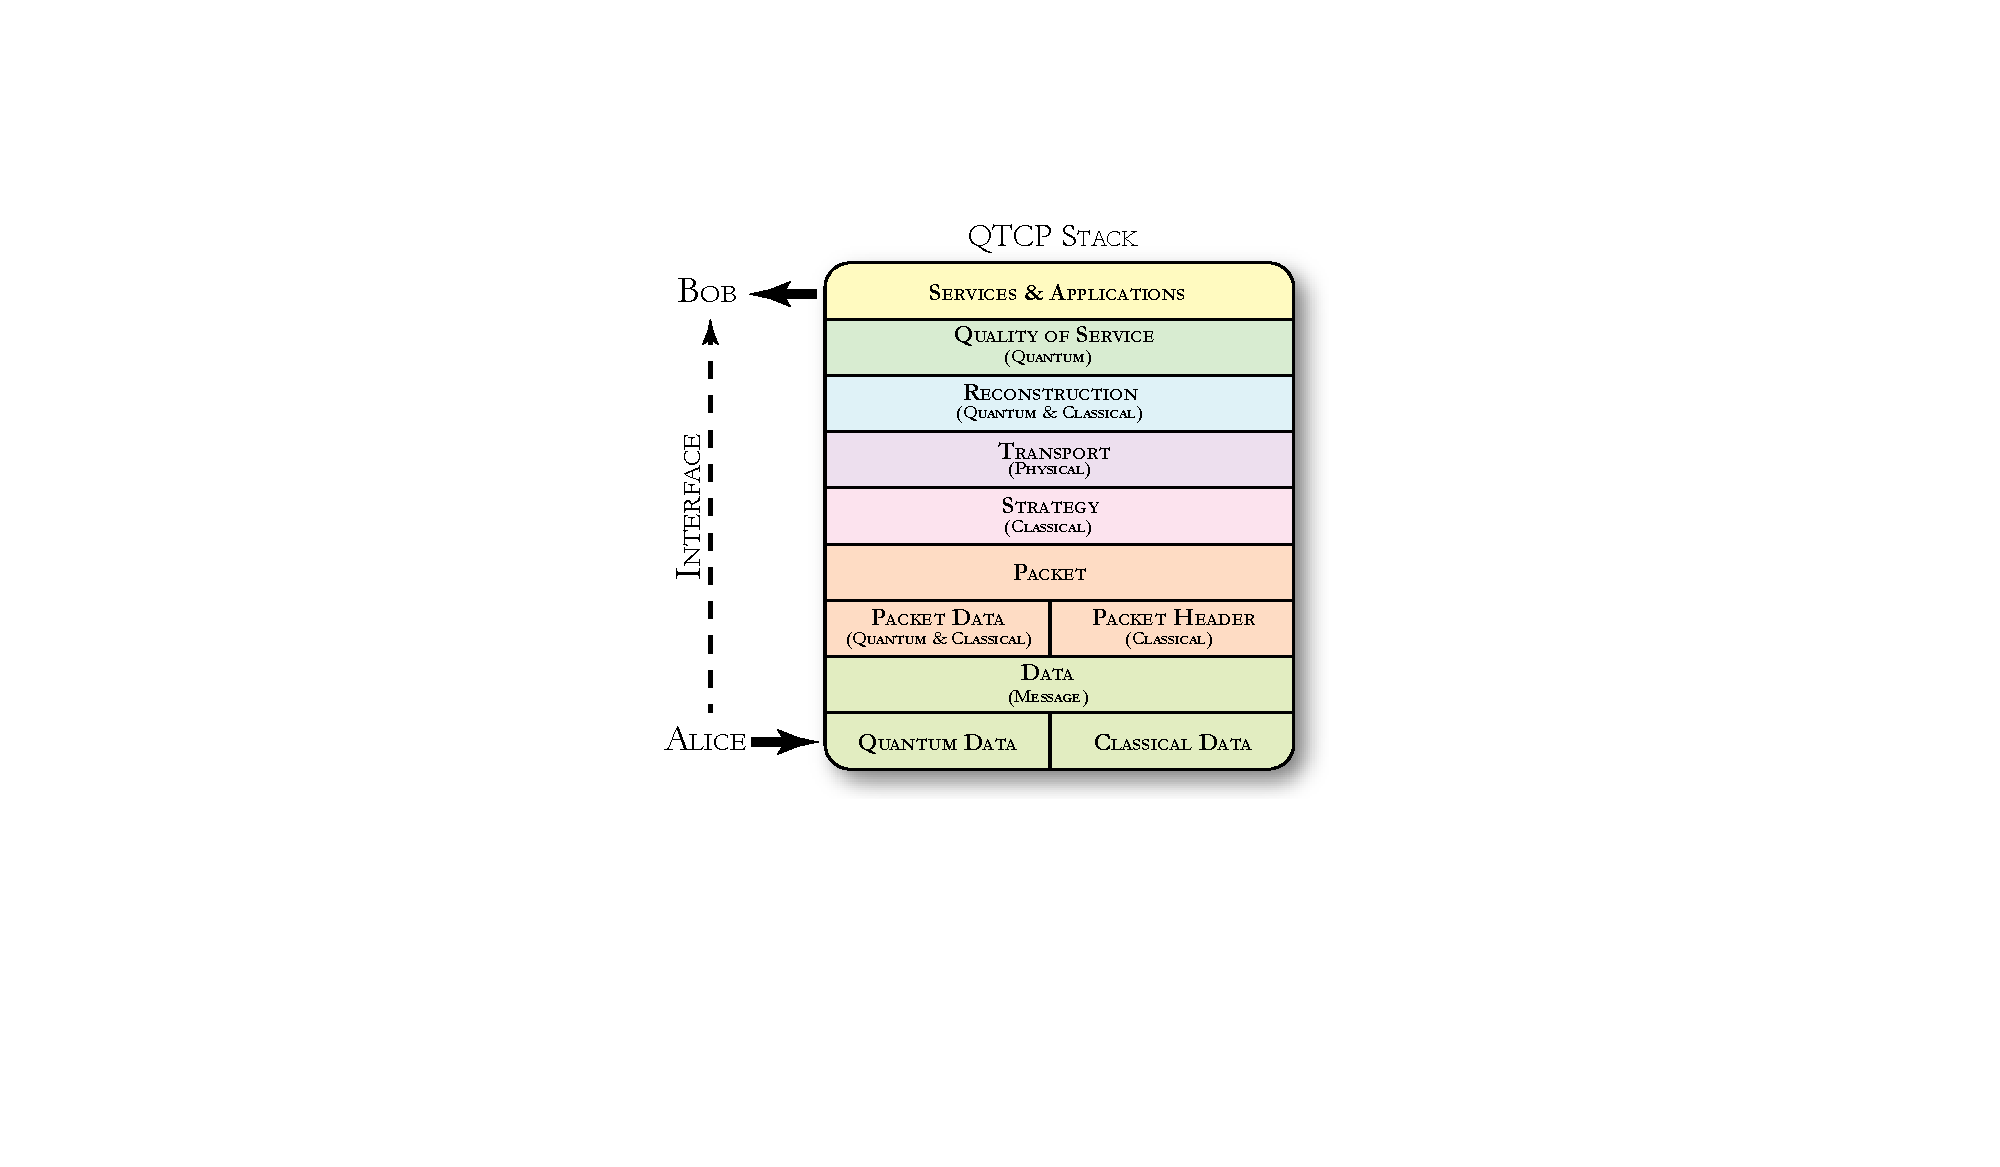
\includegraphics[width=\columnwidth]{stack}
\caption{Protocol stack for QTCP. The protocol stack mediates communication of quantum data from Alice to Bob using the shown layers of abstraction. The end goal is to provide Bob a virtual interface to Alice's transmitted data, while remaining oblivious to the underlying protocol.} \label{fig:stack}
\end{figure}

Next we describe the operation of the layers in the protocol stack in detail.

%
% Data (Message)
%

\subsection{Data (Message)}

At the lowest level of the protocol we have the raw {\sc Data} Alice wishes to communicate to Bob. {\sc Data} is allowed to comprise both {\sc Quantum Data} and {\sc Classical Data} components, and may contain one or the other, or both.

%
% Quantum Data
%

\subsubsection{Quantum data}

{\sc Quantum Data} is allowed to be an arbitrary quantum state. It could be a pure or mixed state, of arbitrary (but predetermined) dimension, or even a subsystem of a larger external state (i.e entangled with another system). We stress that it needn't be expressed using a conventional qubit representation, in the way digital data is necessarily represented using bits. Keep in mind that the quantum internet isn't just there to communicate qubit data streams. Rather, it is intended to act as generally as possible, such that essentially arbitrary \emph{quantum assets} can be exchanged. These needn't be restricted to any particular type of encoding, such as those discussed in Sec.~\ref{sec:opt_enc_of_qi}. For example, in addition to something `standard' like polarisation-encoded qubits in single photons, one network user might like to share an exotic CV state of light, like a cat state, with his mate whose cat died. Indeed, multiple types of state encoding might be encapsulated within a single {\sc Packet}. The QTCP acts only as an abstract interface for quantum networking, but is completely blind as to what the underlying data in the network is. QTCP is only concerned with getting that state from Alice to Bob.

%
% Classical Data
%

\subsubsection{Classical data}

{\sc Classical Data} is a purely classical state with no coherence (i.e a diagonal density matrix), which may be represented as a classical bit-string. We very intentionally segregate the {\sc Classical} and {\sc Quantum} components of {\sc Data}, since the classical network is expected to be cheaper and more reliable than the quantum network operating in parallel to it. The {\sc Classical Data} could, for example, provide nodes with classical instructions on what quantum computations to perform on the {\sc Quantum Data}.

%
% Packet
%

\subsection{Packet}

{\sc Data} is transmitted as {\sc Packets}, much in the same way as conventional TCP. The {\sc Data} is decomposed into three components: {\sc Quantum Data}, {\sc Classical Data}, and {\sc Packet Header}.

We can express the state of an entire {\sc Packet} as,
\begin{align}
\hat\rho_\mathrm{packet}(i) = \hat\rho_\mathrm{quantum}(i) \oplus \hat\rho_\mathrm{classical}(i) \oplus \hat\rho_\mathrm{header}(i),
\end{align}
where $i$ denotes the $i$th packet. Here $\hat\rho_\mathrm{quantum}$ ($\hat\rho_\mathrm{classical}$) is a block of {\sc Quantum Block Size} qubits ({\sc Classical Block Size} bits) taken from the user's {\sc Quantum Data} ({\sc Classical Data}), while $\hat\rho_\mathrm{header}$ is the {\sc Packet's} classical {\sc Packet Header}. As discussed earlier, since $\hat\rho_\mathrm{quantum}$ is quantum, and $\hat\rho_\mathrm{classical}$ and $\hat\rho_\mathrm{header}$ are classical, they needn't be transmitted together over the same quantum network. Instead all {\sc Classical Data} and {\sc Packet Header} could be transmitted over a classical network operating in parallel to and synchronised with the quantum network, which carries the {\sc Quantum Data}.

Note that while one can always measure classical data without disturbance, this is not the case with quantum data, where measurements cause wavefunction collapse. Thus, while Alice is always able to know $\hat\rho_\mathrm{classical}$ and $\hat\rho_\mathrm{header}$, she may or may not know $\hat\rho_\mathrm{quantum}$. Clearly if she prepared the state herself, she would (hopefully) know what she was doing. But in general, quantum networks could be used for far less trivial networking, where Alice is, for example, an intermediary in a distributed quantum computation. In this instance, Alice is unlikely to know what her {\sc Quantum Data} is.

%
% Packet Data
%

\subsubsection{Packet data}

Comprises blocks of both {\sc Quantum Data} and {\sc Classical Data}, of sizes {\sc Quantum Block Size} and {\sc Classical Block Size} respectively. {\sc Packet Data} requires that {\sc Data} be decomposed into distinct subsystems which are independently transmitted by QTCP. We will restrict ourselves to the case where the {\sc Data} is encoded into a stream of qubits ({\sc Quantum Data}) and bits ({\sc Classical Data}). There is no loss of generality in applying this constraint since any quantum (classical) information can be encoded into qubits (bits), and once represented as such, the decomposition of {\sc Data} into {\sc Packets} arises very naturally and intuitively. The {\sc Packet's} {\sc Quantum Data} is what is transmitted via the quantum channels, while the {\sc Classical Data} is communicated via classical channels.

%
% Packet Header
%

\subsubsection{Packet header} \label{sec:packet_header}

{\sc Packet Header} is purely classical and needn't be transmitted over the costly quantum network, instead being transmitted over a complementary classical network, running in parallel to, and synchronised with the quantum network. {\sc Packet Header} contains no information content from {\sc Data}, instead comprising only metadata relevant to the higher levels of the protocol stack. In particular, {\sc Packet Header} contains the following fields:
\begin{itemize}
    \item {\sc Header Size}: The number of bits in the {\sc Packet Header}.
    \item {\sc Message ID}: A unique identifier for the complete message to which this {\sc Packet} belongs. This field mitigates ambiguity as to which {\sc Message} this packet belongs when performing {\sc Reconstruction}.
    \item {\sc Lifetime}: How long the {\sc Packet} has been in existence for, i.e since it was initially sent by the {\sc Sender}. This is used by strategies to prevent collisions.
    \item {\sc Sender}: A unique node identifier for the sender (Alice).
    \item {\sc Recipient}: A unique node identifier for the recipient (Bob).
    \item {\sc Order}: To which block taken from {\sc Data} does this {\sc Packet Data} belong? This is extremely important in networks where {\sc Packets} may arrive out of order. The {\sc Order} field forms the basis for the {\sc Reconstruction} layer.
    \item {\sc Quantum Block Size}: The number of qubits contained in the {\sc Quantum} component of {\sc Packet Data}. This is important for the {\sc Reconstruction} layer.
    \item {\sc Classical Block Size}: The number of bits contained in the {\sc Classical} component of {\sc Packet Data}, also important for the {\sc Reconstruction} layer.
    \item {\sc Routing Queue}: A first in, first out (FIFO) queue of node identifiers, tracing out the entire route for the {\sc Packet} to follow, in chronological order from the next node to visit all the way to the {\sc Recipient}.
    \item {\sc Costs}: A tuple characterising all the accumulated costs of the {\sc Packet} at the current stage in the route. These are treated as accumulators that are incremented appropriately after each step, since costs are additive.
    \item {\sc Attributes}: A tuple characterising all the non-{\sc Cost} properties associated with the {\sc Packet}. Examples include: the {\sc Priority} of routing a {\sc Packet} to its destination; suggesting a preferred routing {\sc Strategy}; or, indicating whether or not a {\sc Resend Until Success} protocol may be applied to this {\sc Packet}.
    \item {\sc Padding}: Null data to pad the joint {\sc Classical Packet Data} and {\sc Packet Header} fields to be of the same length as the {\sc Quantum Packet Data}. This ensures that the components of the {\sc Packet} traversing the quantum and classical channels remain in perfect tandem -- bit for qubit. In Sec.~\ref{sec:transport} we show that this facilitates collision detection without the need to measure quantum states.
    \item {\sc Checksum}: A regular checksum of the entire {\sc Classical} component of the {\sc Packet}, including both {\sc Classical Packet Data} and {\sc Packet Header}. This also forms a part of the collision detection protocol.
\end{itemize}

One might question why {\sc Packet Headers} tally accumulated costs when we ought to already know all the costs, since these were employed by the algorithm for choosing strategies in the first case. In the ideal case where all strategies are determined \emph{a priori} and are implemented as intended, this is certainly valid. However, for generality we retain this option since more realistic networks may require dynamically updating strategies during the course of propagation, in which case dynamically tallying costs is appropriate.

%
% Strategy
%

\subsection{Strategy} \label{sec:into_strat}

Based on the {\sc Packet Headers} of all users sharing the network, choose routing strategies to optimise cost metrics. The notion of strategies is introduced in Sec.~\ref{sec:strat_opt}, and a detailed discussion of example strategies is presented in Sec.~\ref{sec:strategies}.

Once routings have been determined for all {\sc Packets}, the {\sc Routing Queues} in their {\sc Packet Headers} are initialised accordingly by pushing the sequence of node identifiers tracing out the desired route.

In the case of dynamic, time-dependent strategies, which can be updated within the duration of transmissions, the {\sc Routing Queues} may need to be updated. A change in a {\sc Packet's} route simply requires flushing the queue and pushing new node identifiers for each of the nodes in the new route, in chronological order.

The {\sc Strategy} layer is responsible for evaluating the net cost function $f_\mathrm{cost}$ from Eq.~\ref{eq:net_cost_R}, which accounts for both {\sc Costs} and {\sc Attributes} to calculate a single effective cost measure that may be employed in routing decisions.

%
% Transport
%

\subsection{Transport} \label{sec:transport}

The {\sc Transport} layer is responsible for actual routing at the physical level, making direct decisions as to what to do with a {\sc Packet} at each step, based upon the metadata contained in {\sc Packet Header}, most notably the {\sc Routing Queue}, which specifies the full route a {\sc Packet} is destined to follow. It is also responsible for keeping track of costs that accumulate over their route.

Additionally, the {\sc Transport} layer is responsible for collision detection, whereby multiple packets being transmitted simultaneously over a network interfere with one another, corrupting the data. In classical networking, collision detection is straightforward using checksums. But the usual classical approach breaks down in the quantum setting. In Sec.~\ref{sec:collision} we discuss in detail collision detection in QTCP.

The pseudo-code algorithm implemented by the {\sc Transport} layer, including collision detection, is shown in Alg.~\ref{tab:transport_alg}.

\begin{table}[!htb]
\fbox{\parbox{0.965\columnwidth}{\tt
function Transport(Packet):
\begin{enumerate}
    \item nextNode = Packet.RoutingQueue.Pop()
    \item Packet.PhysicallySendTo(nextNode)
    \item Packet.WaitUntilArrivesAt(nextNode)
    \item checksum = Hash(Packet.Header + Packet.ClassicalData)
    \item if(checksum $\neq$ Packet.Header.Checksum) \{
    \setlength{\itemindent}{0.2in}
    \item Packet.Sender.Notify({\sc Failure})
    \item Packet.Recipient.Notify({\sc Failure})
    \item Packet.Discard()
    \item $\Box$
        \setlength{\itemindent}{0in}
\item \}
    \item Packet.Costs += IncomingLink.Costs
    \item Packet.Attributes.Update()
    \item if(Packet.RoutingQueue.Length = 0) \{
    \setlength{\itemindent}{0.2in}
    \item Return(Packet)
        \setlength{\itemindent}{0in}
    \item \}
    \setlength{\itemindent}{0in}
    \item $\Box$
\end{enumerate}}}
\caption{Algorithm implemented by the {\sc Transport} layer of QTCP for each {\sc Packet}. The {\tt Attributes.Update()} function is left undefined. This is where arbitrary {\sc Attribute} dynamics may take place.} \label{tab:transport_alg}
\end{table}

%
% Reconstruction
%

\subsection{Reconstruction}

The {\sc Reconstruction} layer only serves one purpose -- to chronologically reorder the received {\sc Packets} based on the {\sc Order} field in their {\sc Packet Headers}. This stage is only performed by Bob -- the final recipient -- and not at any intermediate stage. In general this will require Bob to have a quantum memory, able to hold all {\sc Packet Data} for a sufficient duration as to enable an arbitrary permutation to be applied, reproducing the correct chronological order.

\begin{table}[!htb]
\fbox{\parbox{0.965\columnwidth}{\tt
function Reconstruction(Packets):
\begin{enumerate}
    \item Packets.WaitUntilAllReceived()
    \item message = Packets.SortByOrderAscending().data
    \item Packets.Receiver.Notify(message)
     \item $\Box$
\end{enumerate}}}
\caption{The goal of the {\sc Reconstruction} layer, is to take a collection of received {\sc Packets} and reassemble them into the {\sc Message}.} \label{tab:reconstruction}
\end{table}

%
% Quality of Service (QoS)
%

\subsection{Quality of service (QoS)} \label{sec:QOS}

In classical networking theory, error detection is an important element of networking protocols. Communication links may be unreliable, or subject to external noise, which users must be able to detect so as to guarantee the quality of their data.

Classically, error detection is typically performed using checksums (hash functions), which generate a short digest of a packet's data that can be recalculated upon arrival to verify integrity. The checksum can be included in the header component of each packet, allowing the remainder of the protocol to remain unchanged.

In the quantum context the elegant notion of checksums is complicated by the fact that calculating a hash function of a quantum state would necessarily entangle the state with the hash function. This would have the undesired effect of causing measurement of the checksum to collapse the quantum state of the data, thereby altering it in an uncontrollable way.

As an alternative to checksums, we could borrow the notion of quantum error correction (QEC) and fault-tolerance from quantum computing theory \cite{???}. Here we encode a quantum state into a (polynomially) larger Hilbert space. \emph{Syndrome measurements} on some of the states in this larger space allow us to both detect and correct universal error models, such as depolarisation or dephasing, provided that error rates are within the fault-tolerance threshold of the code being employed.

QEC codes have been described for protecting against universal error models, including:
\begin{itemize}
\item Pauli errors -- Encompassing dephasing, depolarising and amplitude damping error channels.
\item Qubit loss -- Particularly useful in the optical context where photons are easily lost.
\item Gate failure -- Essential when gates are non-deterministic, necessarily the case when dealing with maximally entangling two-qubit photonic quantum gates.
\end{itemize}

The first described QEC code was the three-qubit code by \cite{bib:Shor95} for redundantly encoding a single logical qubit into three encoded qubits, allowing the detection and correction of at most a single bit-flip error between the encoded qubits. This protocol is shown in Alg.~\ref{tab:three_QEC}. By switching into a Hadamard-rotated basis, the same code could equivalently correct against at most a single phase-flip error (since \mbox{$\hat{H}\hat{X}\hat{H}=\hat{Z}$}). By concatenating these two codes a 9-qubit code correcting against a single depolarising error may be implemented.

Since these original ideas into QEC, countless further codes have been described, able to correct against larger numbers of errors, with far more efficient resource overheads. Currently, topological codes \cite{topologicalCodes} are considered the most favourable codes in terms of their elegance, simplicity, high error-correction thresholds, and efficiency in resource overhead. Some such topological codes are particularly enticing, as they can be readily prepared from cluster states (introduced in Sec.~\ref{sec:CSQC}), which lend themselves naturally to certain networking methods, such as distributed state preparation.

\begin{table}[!htb]
\fbox{\parbox{0.965\columnwidth}{\tt
function ThreeQubitCode($\ket\psi$):
\begin{enumerate}
\item Using two CNOT gates, redundantly encode the logical single-qubit state,
\begin{align}
\ket\psi=\alpha\ket{0}+\beta\ket{1},
\end{align}
into the three-qubit state,
\begin{align}
\ket\psi_R &= \hat{\mathrm{CNOT}}_{1,2}\hat{\mathrm{CNOT}}_{1,3}\ket\psi\ket{00} \nonumber \\
&= \alpha\ket{000}+\beta\ket{111}.
\end{align}
\item Independently apply bit-flip channels $\mathcal{E}_X$ to each of the three encoded qubits.
\item If exactly one bit-flip operation was applied in total, the three possible erroneous encoded states are,
\begin{align}
\ket\psi_1 &= \hat{X}_1 \ket\psi_R = \alpha\ket{001}+\beta\ket{110}, \nonumber \\
\ket\psi_2 &= \hat{X}_2 \ket\psi_R = \alpha\ket{010}+\beta\ket{101}, \nonumber \\
\ket\psi_3 &= \hat{X}_3 \ket\psi_R = \alpha\ket{100}+\beta\ket{011}.
\end{align}
\item Using three pairs of CNOT operations and $\hat{Z}$-basis measurements, apply parity measurements between each of the three pairs of encoded qubits.
\item Assuming at most a single bit-flip operation has occurred on the encoded state, the three parity outcomes uniquely determine which encoded qubit the bit-flip was applied to.
\item Apply classically-controlled bit-flip recovery operations, $\mathcal{R}$, to correct the encoded state, recovering $\ket\psi_R$.
\item Apply the inverse of the encoding operation to recover $\ket\psi$.
\item $\Box$
\end{enumerate}
\begin{align}
\Qcircuit @C=1.3em @R=.6em {
  & \lstick{\ket{\psi}} & \ctrl{2} & \gate{\mathcal{E}_X}  & \qw & \qw              & \ctrl{3}  & \qw       & \ctrl{4} & \qw & \multigate{2}{\ \mathcal{R}\ } & \qw \\
  & \lstick{\ket{0}}    & \targ    & \gate{\mathcal{E}_X}  & \qw & \qw              & \ctrl{2}  & \ctrl{2}  & \qw      & \qw & \ghost{\ \mathcal{R}\ } \qw & \qw \\
  & \lstick{\ket{0}}    & \targ    & \gate{\mathcal{E}_X}  & \qw & \qw              & \qw       & \ctrl{2}  & \ctrl{3} & \qw & \ghost{\ \mathcal{R}\ } \qw & \qw \\
  &          &          &          & & \lstick{\ket{0}} & \targ \qw & \qw       & \qw      & \meter & \control \cw \cwx \\
  &          &          &          & & \lstick{\ket{0}} & \qw       & \targ \qw & \qw      & \meter & \control \cw \cwx \\
  &          &          &          & & \lstick{\ket{0}} & \qw       & \qw       & \targ    & \meter & \control \cw \cwx
} \nonumber
\end{align}
}}
\caption{Three-qubit code for protecting against at most a single logical bit-flip error.} \label{tab:three_QEC}
\end{table}

Different error correcting codes have different error correcting power, and different resource overheads, which must be taken into consideration. The appropriate choice of code will largely be determined by the final {\sc Services \& Applications} layer. For some simple quantum communications protocols, simple error correction (or even no error correction) may suffice. A full-fledged quantum computation on the other hand will require error rates within a fault-tolerance thresholds.

The field of fault-tolerance is already extremely well developed and could be applied directly to QTCP as an abstraction layer directly below the {\sc Services \& Application} layer of the protocol stack -- the {\sc QoS} layer -- abstracting it away from the end-user. The transport layer protocol for applying it to the QTCP stack in Alg.~\ref{tab:qos}.

\begin{table}[!htb]
\fbox{\parbox{0.965\columnwidth}{\tt
function QoS(Packets):
\begin{enumerate}
    \item qec = Packets.ApplyQEC()
    \item if(qec.success = true) \{
    \setlength{\itemindent}{0.2in}
    \item message.Receiver.Notify(qec.data)
    \setlength{\itemindent}{0in}
    \item \} else \{
    \setlength{\itemindent}{0.2in}
    \item message.Receiver.Notify({\sc Failure})
    \setlength{\itemindent}{0in}
    \item \}
    \item $\Box$
\end{enumerate}}}
\caption{QoS algorithm based on any appropriate existing QEC code.} \label{tab:qos}
\end{table}

%
% Services & Applications
%

\subsection{Services \& applications}

Having communicated all the {\sc Packet Data} from Alice to Bob, performed {\sc Reconstruction}, and applied {\sc QoS} protocols, Bob ought to have $\hat\rho_\mathrm{data}$ to a good approximation. The quality of Bob's received state can be inferred directly from the {\sc Costs} vector contained in the {\sc Packet Headers}. The final state and its associated quality metrics ({\sc Costs} and QEC outcomes) may then be provided to Bob as a software interface for end use.

%
% Collision Handling & Classical Errors
%

\section{Collision handling \& classical errors} \label{sec:collision}

In classical networking, protocols such as Ethernet allow users to simply broadcast data at their leisure and rely on \emph{collision detection} to detect when the broadcasts of multiple users have interfered, signalling that both users ought to retransmit following backoff, to minimise the chances of another collision occurring. While this {\sc Resend Until Success} approach has certainly proven to be effective in classical networking, in a quantum setting the rules of the game are entirely different.

First, collision detection necessarily requires measuring a communications channel to test whether data has been corrupted. Classical networks typically do this by transmitting a checksum with the data, which is recalculated upon arrival for comparison. This raises the obvious problem that quantum measurements are destructive, which means that testing the integrity of our data destroys it in the process -- the last feature we'd like our network to exhibit! However, to overcome this, in Sec.~\ref{sec:transport} we describe a protocol based on the dual classical/quantum network that allows collision detection without measuring quantum states.

Second, collision detection is not always even allowed at all. If one of Alice's packets was entangled with another (i.e she was communicating an entangled system, where the different subsystems resided in different packets), she would not be able to simply retransmit an identical copy of the corrupted packet, since the entanglement with the other system would have been lost and there are no local operations she can do to recover it.

Alternately, Alice might be a part of a distributed computation, where she didn't prepare the data in the first place. In this instance, the no-cloning theorem implies that she cannot, in general, learn what the quantum state was, and therefore would be unable to make a second transmission attempt.

From Alice's point of view, {\sc Resend Until Success} would clearly work if she was preparing a known separable state. However, collisions on the network caused by her reckless resending would likely corrupt the communications between other parties, leaving them rather ticked off at her.

There are therefore two main approaches to dealing with collisions. First, central planning of all routing could be employed, precisely scheduling all routes \emph{a priori} so as to entirely eliminate any possibility for collisions. Second, if all users in the network were communicating data where packet loss could be tolerated, they could all mutually agree to use the {\sc Resend Until Success} protocol. This would not require a central authority, and be highly desirable for ad hoc networks. It is important to stress, however, that the latter requires unanimity amongst network participants to function, and the restriction to known, separable states is a major limitation that would prohibit many important uses for quantum networks, such as distributed quantum computation. However, both these approaches are entirely valid in their appropriate context.

In classical TCP all components of data packets are classical and are kept together throughout every stage of transmission. In the quantum case we will instead have a mixture of both quantum and classical data. As mentioned, we will assume that classical communication and computation resources `come for free' (or are at least cheap compared to quantum resources), so there will be a clear disambiguation as to what data is quantum or classical within packets.

As discussed, quantum collision detection is complicated by the fact that measuring quantum data to determine whether it has been corrupted disturbs the quantum state. We address this problem by taking advantage of the duality of the quantum/classical network, discussed in Sec.~\ref{sec:quant_net}. Because the quantum and classical components of the {\sc Packets} are synchronised and of equal length (thanks to the {\sc Padding} field of the {\sc Packet Header}), and because the same applies to all other {\sc Packets} on the network, a collision in the quantum data necessarily implies a collision in the classical data, and vice versa. Therefore, by applying regular classical collision detection techniques based on checksums (recall {\sc Packet Header} contains a {\sc Checksum} field), we can infer collisions in quantum data without actually measuring it. We refer to this as \emph{indirect collision detection}. This guarantees us the ability to detect when a collision has occurred, in which case both quantum \emph{and} classical data are corrupted, or has not occurred, in which case both quantum and classical data are uncorrupted and the quantum data remains unmeasured. Collision detection is incorporated into the pseudo-code implementation of the {\sc Transport} layer shown in Alg.~\ref{tab:transport_alg}.

This algorithm could, depending upon implementation, be executed locally on the node currently hosting the {\sc Packet}, or it could be delegated to a central authority, but with the overhead of additional classical communication.

In instances where corruption or loss of packets cannot be tolerated, a more proactive approach may be applied. To preempt the risk of packet collision, one could introduce \emph{probe packets} -- packets containing only classical data, that query a route ahead to negotiate channel usage for the following proper packet, thereby avoiding collisions. Of course, if an upcoming node is unable to guarantee channel capacity immediately, the packet may need to be stored in quantum memory until the channel is available. Thus, it is important to accommodate for this by ensuring that quantum memory is available in nodes preceding links/nodes where collisions are not guaranteed to be mitigated immediately. Quantum memory will be discussed in Sec.~\ref{sec:memory}.

%
% Strategies
%

\section{Strategies} \label{sec:strategies}

In Sec.~\ref{sec:costs} we introduced the notion of network costs, strategies for allocating network resources in Sec.~\ref{sec:route_strats}, and a general formalism for optimising strategies so as to minimise costs in Sec.~\ref{sec:strat_opt}. In this section we present some meaningful example strategies and associated pseudo-code fragments, illustrating the implementation of various aspects of strategies of practical real-world interest.

%
% Single User (Shortest-Path)
%

\subsection{Single user} \label{sec:single_user_shortest}

Let us begin our discussion of strategies by considering the simplest case of just a single user on the network. Consider the graph shown in Fig.~\ref{fig:simp_route_opt}. This is the same example used earlier, but now the edges have been weighted by some arbitrary cost metric. There are four routes from $A$ to $B$. All have cost \mbox{$c=3$} except the route indicated by the red arrow, which has cost \mbox{$c=2$}. Clearly the latter is optimal in terms of cost minimisation, and any shortest-path algorithm applied between $A$ and $B$ will accurately come to that conclusion. Thus, single-user networks are very trivial to optimise, and there is no distinction between {\sc Local} and {\sc Global} strategies.

The very trivial algorithm for this route finding is shown in Alg.~\ref{tab:single_user}, where the {\tt ShortestPath()} function could be any of the existing, well-known shortest path algorithms (Sec.~\ref{sec:shortest_path}).
\begin{table}[!htb]
\fbox{\parbox{0.965\columnwidth}{\tt
function Strategy.SingleUser(Packets):
\begin{enumerate}
    \item foreach(packet in Packets) \{
        \setlength{\itemindent}{.2in}
                \item currentNode = packet.RoutingQueue.Pop()
        \item shortestRoute = \\
        ShortestPath(currentNode,packet.Recipient)
        \item packet.RoutingQueue.Flush()
        \item packet.RoutingQueue.Push(shortestRoute)
    \setlength{\itemindent}{0in}
    \item \}
    \item $\Box$
\end{enumerate}}}
\caption{For a single user, a simple shortest-path algorithm necessarily finds the optimal route, as there is no potential for packet collisions or competition for network resources.} \label{tab:single_user}
\end{table}

%
% Multiple Users
%

\subsection{Multiple users} \label{sec:two_user}

Next consider the more complex network shown in Fig.~\ref{fig:conflict}. We consider two pairs of sender/receiver, \mbox{$A_1\to B_1$} and \mbox{$A_2\to B_2$}. The available routes connecting both pairs overlap, creating competition for network resources.

Let us assume there are just two properties of interest when deciding strategies -- cost in dollars (which may differ for different links), and availability (i.e how many states can the channel handle at once). Let $c_1$ be the dollar cost, and \mbox{$a_1$} be the amount of available channel capacity. Our network is very primitive and each channel can only accommodate one state at a time. Thus, we let \mbox{$a_1=1$} for all links, except for the one common to both $R_1$ and $R_3$, \mbox{($R_1\cap R_3$)}, which we invest more heavily into, since both routes are going to be wanting to use this link.

To define our net cost measure, we combine $c_1$ and $a_1$ according to,
\begin{align}
\mathcal{S} : f_\mathrm{net}(\vec{c}) = \left\{
\begin{array}{l l}
c_1 & \quad \mathrm{if}~ a_1>0 \\
\infty & \quad \mathrm{if}~~ a_1=0 \\
\end{array} \right..
\end{align}
That is, provided bandwidth is available, the link will have the dollar cost $c_1$. If no bandwidth is available, the cost is infinite, thereby removing the respective link from the graph.

Next the cost metrics are updated by the strategy $\mathcal{S}$ following each communication. In this instance this simply decrements the bandwidth attribute for the links that were utilised,
\begin{align}
\mathcal{S} : a_1 \to a_1-1.
\end{align}
Suppose the strategy optimises the \mbox{$A_1\to B_1$} route first, yielding $R_3$, before moving onto the \mbox{$A_2\to D_2$} route. In this case, the reduction of the bandwidth attribute signals that the cheapest route $R_2$ is no longer available to be utilised simultaneously to $R_3$, and must therefore wait its turn on the following clock cycle. Alternately, the strategy could employ $R_1$ for \mbox{$A_2\to B_2$}, in which case their common link with capacity for two states would eliminate the competition between the two communications, allowing both to take place simultaneously. Thus, there is a tradeoff: for \mbox{$A_2\to B_2$}, we could achieve a net cost of \mbox{$c(A_2\to B_2)=5$}, requiring 2 clock cycles; or we could achieve simultaneous communication at the expense of increasing cost to \mbox{$c(A_2\to B_2)=6$}. This indicates that when choosing strategies, we must carefully define its goals.

Suppose net cost, rather than clock cycles, was the key measure of interest. Then choosing the routes $R_1$ and $R_3$ would be the optimal choice. An optimal {\sc Global} optimisation would recognise this. However, a {\sc Local} optimisation, based on choosing shortest-paths one-by-by for each sender/receiver pair, may or may not choose the optimal routes, depending on the order in which the decisions were made.

Suppose the \mbox{$A_2\to B_2$} route were optimised first. We would choose $R_2$. Then there would be a traffic jam on the \mbox{$A_1\to B_1$} route, and it would necessarily have to wait its turn. In a time-critical application, where waiting is intolerable, this effectively renders the network useless to the first sender/receiver pair.

If, however, the \mbox{$A_1\to B_1$} were optimised first, choosing $R_3$, then $R_2$ would be prohibited once the bandwidth attributes were updated, and the second best option, $R_1$, would be chosen. Now both communications could take place simultaneously. So we see that the outcomes of {\sc Local} optimisations needn't always be consistent or unique. Rather, they can be highly dependent upon circumstantial issues, such as the arbitrary order in which routes are chosen for optimisation.

\begin{figure}[!htb]
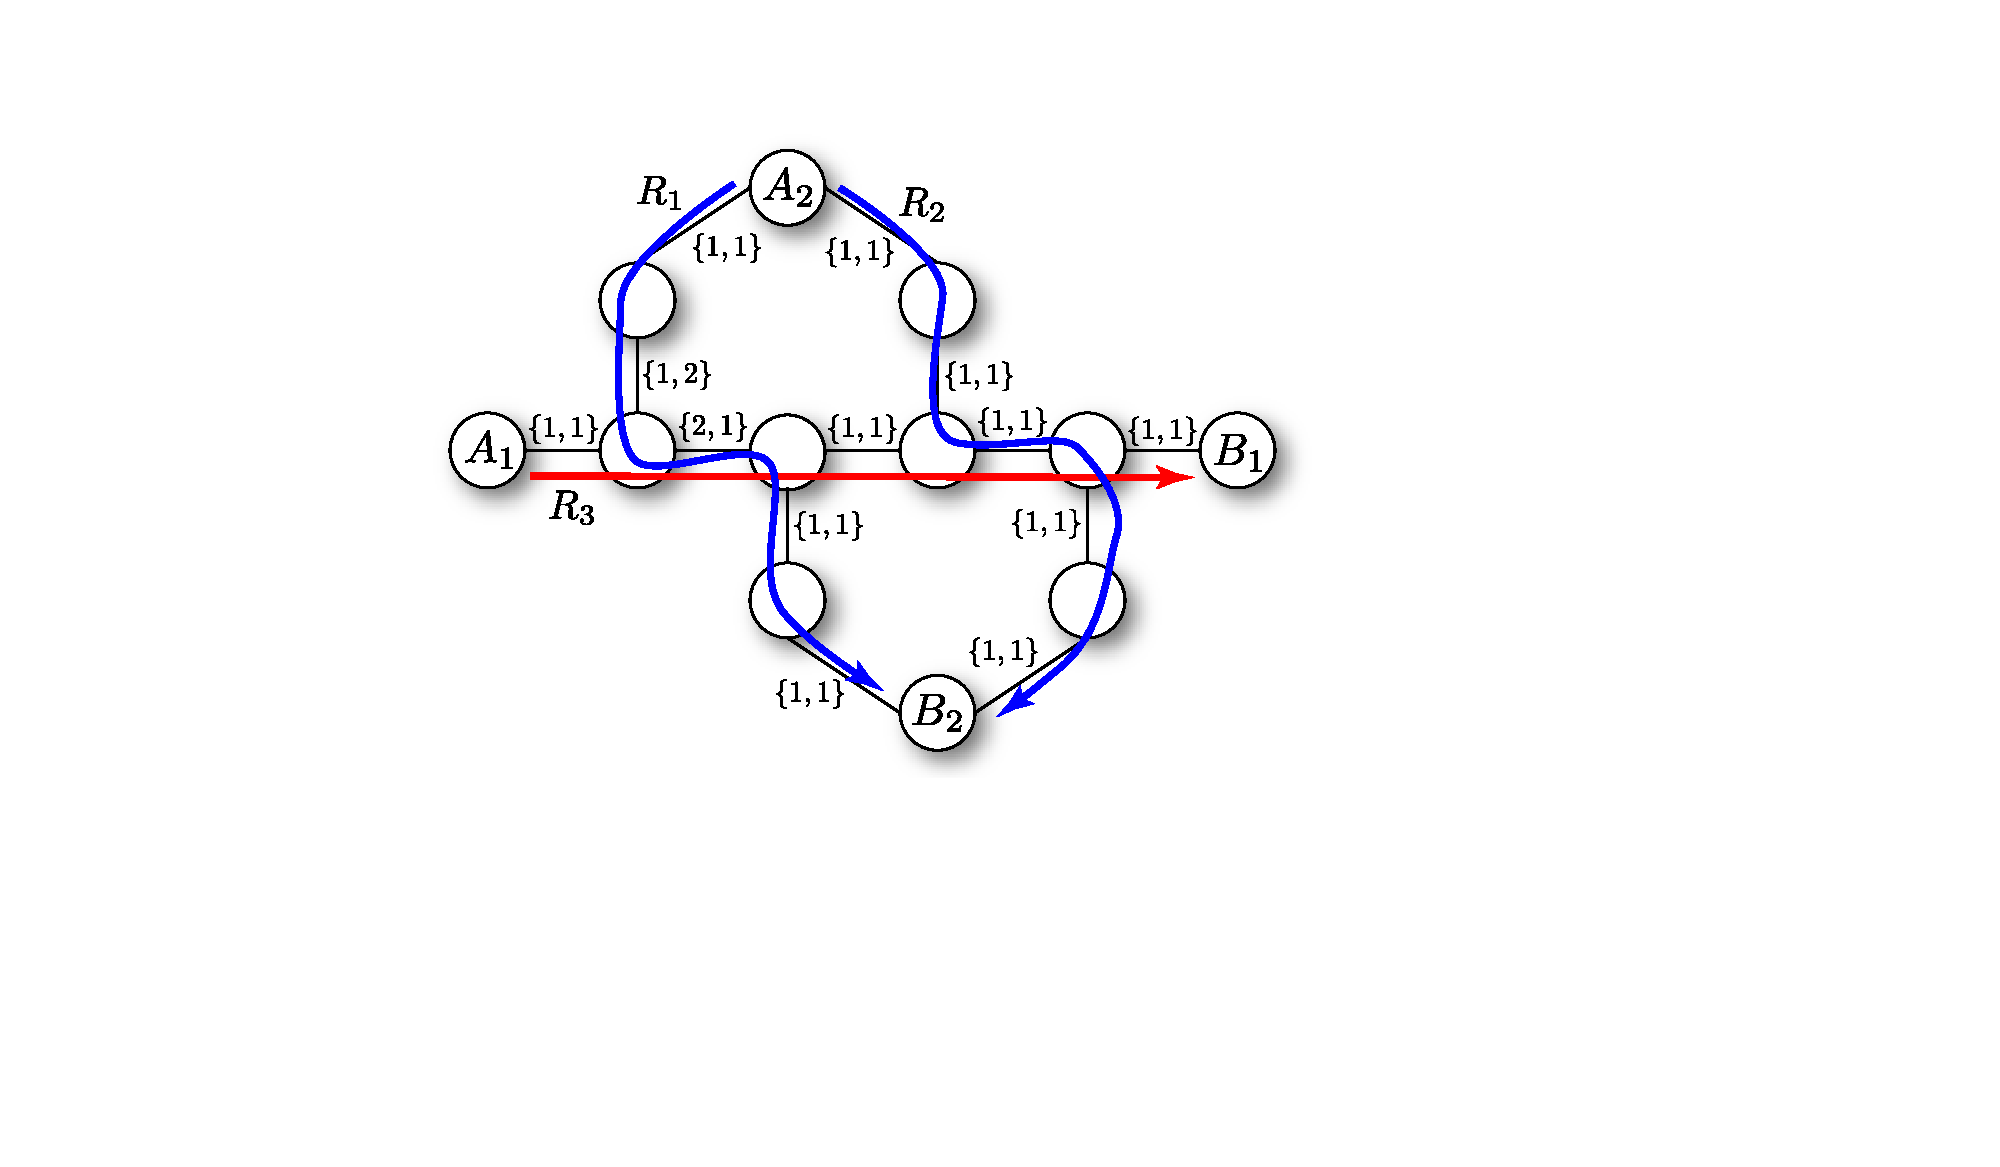
\includegraphics[width=\columnwidth]{conflict}
\caption{A simple network with two competing pairs of senders and receivers, \mbox{$A_1\to B_1$} and \mbox{$A_2\to B_2$}. Edges are labelled by \mbox{$\{b,d\}$}, where $b$ is the bandwidth attribute of the link (i.e number of states that can be communicated simultaneously), and $d$ is the cost metric associated with the link, e.g loss in dB. (blue line) $R_1$ and $R_2$ are two routes from $A_2\to B_2$. Either of these routes could be declared optimal, depending on the choice of cost function. (red lines) $R_3$ is the optimal route from \mbox{$A_1\to B_1$}.} \label{fig:conflict}
\end{figure}

Generalising this to any number of users is a straightforward extension to the route optimisation problem, incurring a higher computational overhead due to the increased optimisation complexity.

In the upcoming sections we discuss multi-user strategies in more detail. None of these are true {\sc Global} strategies, but nonetheless address some of the problems facing {\sc Local} strategies mentioned above.

%
% Round Robin
%

\subsection{Round robin} \label{sec:round_robin}

Perhaps the simplest and most elegant multi-user scheduling strategy is to borrow from the idea of time-division multiplexing for preemptive multitasking employed by UNIX operating systems. Here we simply put all live packets in a list, and go through the list, one-by-one, giving each packet an equal time-share of network resources, independent of costs. The algorithm for this is shown in Alg.~\ref{tab:round_robin}.

\begin{table}[!htb]
\fbox{\parbox{0.965\columnwidth}{\tt
function Strategy.RoundRobin(Packets):
\begin{enumerate}
    \item foreach(packet in Packets) \{
        \setlength{\itemindent}{.2in}
                \item currentNode = packet.RoutingQueue.Pop()
        \item shortestRoute = \\
        ShortestPath(currentNode,packet.Recipient)
        \item packet.RoutingQueue.Flush()
        \item packet.RoutingQueue.Push(shortestRoute)
    \setlength{\itemindent}{0in} \}
    \item $\Box$
\end{enumerate}}}
\caption{In the {\sc Round Robin Strategy} we simply iterate through the list of active packets, with no regard for any metrics, or conflicts between them. Rather, we strive for perfect time-sharing equality, and every packet entirely ignores the actions of all other packets.} \label{tab:round_robin}
\end{table}
The {\sc Round Robin} strategy can be considered base skeleton code for more sophistic algorithms to build upon, simply by reordering the packet queue.

While such a protocol clearly ensures scheduling that gives all packets attention, it is the perfect example of an algorithm subject to the resource allocation imbalance discussed in Sec.~\ref{sec:two_user}. Specifically, the routes being followed by some packets may systemically receive more favourable treatment than others, based on the ordering of the list of packets. Also, equal timesharing fails to accommodate for the fact that some routes are inherently more costly than others and deserve a greater share of network resources.

%
% Data Priority
%

\subsection{Data priority} \label{sec:data_priority}

Are all men created equal? No. Some packets may inherently be more important than others, and ought to receive priority when allocating network resources. A simple variation on the {\sc Round Robin} strategy is to, before iterating through the list of packets, order them according to a {\sc Priority} attribute. Thus, when applying a shortest-path algorithm, it is deemed most important to minimise the costs of the more important packets first.

This is trivially achieved by taking the existing {\sc Round Robin} strategy, and first ordering the packet list by their priority attributes, i.e by inserting a new line 1, \mbox{\tt Packets.SortByPriority()}.

%
% Randomisation
%

\subsection{Randomisation} \label{sec:random}

The imbalance issue facing the {\sc Round Robin} strategy (Sec.~\ref{sec:round_robin}) may be most trivially addressed using randomisation of the strategy, such that routes are optimised in an order chosen randomly each time. This would allow the different sender/receiver pairs to have equal access to network resources, when averaged over many network uses.

This is also straightforward variation of the {\sc Round Robin} strategy, achieved by first randomising the list of packets before the other stages, i.e insert a new line 1, \mbox{\tt Packets.RandomizeOrder()}.

%
% Cost Priority
%

\subsection{Cost priority} \label{sec:cost_priority}

The {\sc Random} strategy overcomes one key problem facing any {\sc Local} optimisation strategy. But it is nonetheless merely a mild variation on the {\sc Round Robin} strategy, guaranteeing equal time-share to each sender/receiver pair. But does equal time-sharing actually represent the best allocation of resources?

It isn't just the order in which routes are chosen which creates imbalance between users. The costs and attributes of the routes themselves is inevitably biased more in favour of some users than others. To accommodate this we now introduce the {\sc Cost Priority} strategy. Here, rather than prioritising packets on a random basis, or according to a fixed, predetermined priority attribute, we do so according to their net accumulated cost. Those who have accumulated the highest cost will subsequently be treated with highest priority. This strategy effectively introduces a negative feedback loop into resource allocation, creating a self-regulating (and hopefully stable!) time-multiplexed packet-switched network. The pseudo-code for the {\sc Cost Priority} strategy is shown in Alg.~\ref{tab:cost_prior_alg}.

\begin{table}[!htb]
\fbox{\parbox{0.965\columnwidth}{\tt
function Strategy.CostPriority(Packets):
\begin{enumerate}
    \item packetsAndCosts = []
    \item foreach(packet in Packets) \{
        \setlength{\itemindent}{.2in}
        \item cost = costFunction(packet)
        \item packetsAndCosts.Append([packet,cost])
    \setlength{\itemindent}{0in}
    \item     \}
    \item sorted = \\
        SortByCostDescending(packetsAndCosts)
    \item foreach(packet in sorted) \{
        \setlength{\itemindent}{.2in}
        \item currentNode = packet.RoutingQueue.Pop()
        \item shortestRoute = \\
        ShortestPath(currentNode,packet.Recipient)
        \item packet.RoutingQueue.Flush()
        \item packet.RoutingQueue.Push(shortestRoute)
    \setlength{\itemindent}{0in}
    \item \}
    \item $\Box$
\end{enumerate}}}
\caption{The {\sc Cost Priority Strategy} scheduling algorithm that gives highest routing priority to {\sc Packets} with the highest accumulated cost (i.e which have suffered the most). The as-yet undefined {\tt costFunction()}, which refers to $f_\mathrm{cost}$ from Eq.~\ref{eq:net_cost_R}, is where the details of the priority decisions are made, which could be entirely arbitrary. In this example, the shortest route is recalculated at each step, based on the expectation that network metrics are dynamic.} \label{tab:cost_prior_alg}
\end{table}

This is an example of a {\sc Greedy} optimisation algorithm, which attempts to optimise routing by always optimising the most desperate packets first, in descending order down to the least. It is well-known that {\sc Greedy} algorithms often do not find global optima. Nonetheless, this approach improves on the previous multi-user protocols.

Let us consider a simple example scenario. Imagine we begin with an ordinary network graph, with edges weighted by costs and attributes. For generality, we will additionally assume the available network resources are very dynamic and unpredictable. The costs associated with links are at the whim of market forces we do not understand (do we ever?). And, for the sake of example, and to make matters worse, the links have been very unreliable lately, and are routinely dropping in and out -- `blackouts'. This effectively rules out \emph{a priori} route optimisation, requiring something dynamic.

There are many users on the network, with many active packets at any give time, but because of the constant oscillations in network resources, some packets have received second-class treatment, and through neglect accumulated an unfair share of state degradation. This simple toy model is, at least qualitatively, something that could arise quite naturally in networks with constrained or unreliable resources.

Let us define an example {\sc Cost Priority} strategy using the following:
\begin{itemize}
\item {\sc Latency Cost}: How long has the packet has been in transit for? This is actually a very general cost metric, since any other cost metric measured in units per time will be directly proportional to this metric. That is, loss, fidelity, purity, efficiency, and so on, all mirror this metric when expressed on a decibel scale. Of course, the same strategy could have easily been applied to any other cost metric.
\item {\sc Blackout Attribute}: Is our unreliable link actually working right now? A given link will have probability $p_\mathrm{op}$ of being operational at any given time, chosen independently for each link at each clock-cycle. The {\tt Attributes.Update()} function from Alg.~\ref{tab:transport_alg} is responsible for implementing this.
\item \mbox{\sc Cost Function} ($f_\mathrm{cost}$, {\tt costFunction()} in Alg.~\ref{tab:cost_prior_alg}): The strategy must make sensible decisions based upon only the above two parameters. Because the previously mentioned generality of the {\sc Latency} metric, we would like the net cost to directly reflect this metric, but only of course, if the link is operational. If it is not, then that link must be ruled out entirely by assigning it an infinite cost. Thus, we simply choose,
\begin{align}
\mathcal{S} : f_\mathrm{cost}(c,a) = \left\{
\begin{array}{l l}
c & \quad \mathrm{if}~ a=\mathrm{\tt True} \\
\infty & \quad \mathrm{if}~ a=\mathrm{\tt False} \\
\end{array} \right..
\end{align}
Note that different packets could be associated with different net cost functions, $f_\mathrm{net}$, to accommodate for the different QoS requirements of different users and messages.
\end{itemize}

In other words, the net cost is taken directly from the underlying cost metric, and modulated by an attribute, yielding a net cost for each packet, which is used to determine which packets receive priority.

This provides us with a simple illustration of how costs and attributes can compliment one another to yield meaningful strategies, that improve network performance over na\"ive, but well-intentioned, time-sharing approaches.

%
% All or Nothing
%

\subsection{All or nothing} \label{sec:all_or_nothing}

In some cases, end-user applications may have strict QoS constraints associated with any data they receive. For example, in a time-critical enterprise, say high-frequency trading, receiving information a millisecond too late is worthless, and it would be best to discard the out of date information to free up bandwidth for the next round of information. Alternately, if the fidelity of a state is required to strictly fall within a fault-tolerance threshold, it will be useless if the threshold is violated. In such a context, the {\sc Strategy} will apply hard boundaries on QoS metrics, discarding anything violating it, after which some other {\sc Strategy} is applied. The algorithm is summarised in Alg.~\ref{tab:all_or_nothing}.

\begin{table}[!htb]
\fbox{\parbox{0.965\columnwidth}{\tt
function Strategy.AllOrNothing(Packets, threshold):
\begin{enumerate}
    \item foreach(packet in Packets) \{
        \setlength{\itemindent}{.2in}
        \item cost = costFunction(packet)
        \item if(cost $\geq$ threshold) \{
        \setlength{\itemindent}{.4in}
            \item packet.Sender.Notify({\sc Failure})
            \item packet.Recipient.Notify({\sc Failure})
            \item Packets.Discard(packet)
                    \setlength{\itemindent}{.2in}
            \item \}
        \setlength{\itemindent}{0in}
    \item \}
    \item Strategy.SomeOtherStrategy(Packets)
    \item $\Box$
\end{enumerate}}}
\caption{The {\sc All or Nothing Strategy}. If the net cost of a packet exceeds a certain {\tt threshold}, it is discarded outright, and the sender and recipient notified.} \label{tab:all_or_nothing}
\end{table}

%
% Optimal Flow
%

\subsection{Optimal flow}

In Sec.~\ref{sec:flow_networks} we introduced flow networks as a means for analysing networks where maximising network flow (throughput) is the primary objective. Formulating our quantum networks in this manner is extremely convenient since, combined with our existing definitions for cost metrics and attributes, we can easily exploit a plethora of known results from flow network theory.

As an example of how load allocation might be applied in a simple network, consider again the network shown in Fig.~\ref{fig:simp_route_opt}, where the edge weights are regular cost metrics (not capacities). Alice wishes to send two packets to Bob, simultaneously if possible. Clearly she would transmit her first packet over the \mbox{$A\to F\to B$} route, since this has lowest cost. But let us assume that every link has a maximum capacity of one packet per unit time. In this case Alice will be unable to send her second packet via the same route and must instead resort to using \mbox{$A\to C \to B$} or \mbox{$A\to D\to B$}. The optimisation is straightforward in this instance. However, in general these types of optimisations are somewhat more involved.

These scenarios are handled by flow network optimisation algorithms, of which there are many. We discuss a few of the most relevant ones for our purposes in Sec.~\ref{sec:graph_theory}. Note that these algorithms are {\sc Global} optimisation algorithms, requiring complete knowledge of the status of the entire network to perform the optimisation.

The routing strategy is very straightforward, shown in Alg.~\ref{tab:opt_flow}, since the {\sc Global} flow-optimisation algorithm completely specifies the entire configuration of routes through the network.

\begin{table}[!htb]
\fbox{\parbox{0.965\columnwidth}{\tt
function Strategy.OptimalFlow(Packets):
\begin{enumerate}
    \item routes = Packets.OptimalFlowRoutes()
    \item foreach(packet in Packets) \{
        \setlength{\itemindent}{.2in}
                \item packet.RoutingQueue.Flush()
                \item packet.RoutingQueue.Push(routes[packet])
    \setlength{\itemindent}{0in} \}
    \item $\Box$
\end{enumerate}}}
\caption{A generic optimal flow routing strategy. {\sc Packets} is the array of all packets that ought to be transmitted simultaneously, which are collectively optimised using some flow optimisation algorithm before undergoing transport.} \label{tab:opt_flow}
\end{table}

%
% Extensibility of QTCP
%

\section{Extensibility of QTCP} \label{sec:c_vs_a}

In Sec.~\ref{sec:costs} we introduced the notion of the \emph{costs} and \emph{attributes} of links in a classical network, and in Sec.~\ref{sec:quantum_meas_cost} generalised these notions to the quantum case. In Sec.~\ref{sec:packet_header} we described the header format for quantum packets.

The {\sc Costs} and {\sc Attributes} fields within the {\sc Header} are very powerful data structures, implemented as ordered sets of arbitrary dimension, comprising arbitrary data fields. The intention here is to allow QTCP to be extensible into the future, with the addition of new data structures into the protocol. These can be custom designed to, in conjunction with appropriate routing strategies and cost functions, influence the operation of QTCP completely arbitrarily, and easily implement entirely different quantum networking paradigms than presented here.

{\sc Costs} naturally capture characteristics of the network that accumulate additively along routes, whereas {\sc Attributes} capture any other characteristics that aren't additive. A network needn't have both costs \emph{and} attributes. It may have one or the other, or both, but not neither, since there must be some measure by which to judge routes.

%
% Scalability
%

\section{Scalability of QTCP}

\comment{To do}

\comment{Discussion of how QTCP protocol/policies might be designed to change with scale. E.g for a small LAN the policies/metrics/attributes might be completely different than for an intercontinental uplink. Discuss how this scalability might be implemented, with examples.}

%
% Message- vs. Packet-Level Routing
%

\section{Message- vs. Packet-Level Routing}

\comment{To do}

\comment{Limit of packet$\to$message size. How does this change strategy.}

%
% Interconnecting & Interfacing Quantum Networks
%

\section{Interconnecting \& interfacing quantum networks} \label{sec:inter}

Any global-scale network will inevitably comprise participants choosing to go about things their own way. The physical architecture and medium may vary from one subnetwork to the next, as may the QTCP policies they adopt. The key then is to construct efficient \emph{interconnects} between different levels of the network hierarchy, each of which may subscribe to their own QTCP policies and cross between different physical mediums. Note that the QTCP protocol presented here does not enforce any particular networking policies, but rather provides a high-level framework that can be customised essentially arbitrarily.

For example, the cost metrics and attributes employed at the intercontinental level would most certainly be very different to those in a small LAN. A small LAN might be running applications whereby they can easily reproduce packets and thereby tolerate packet loss. But for a warehouse-scale commercial quantum computing enterprise, responsible for performing one stage of a distributed quantum computation, the loss of a single packet could be extremely costly, requiring the entire computation to be performed completely from scratch due to no-cloning and no-measurement limitations, something that may not come cheaply.

Such interconnects will typically comprise a combination of:
\begin{itemize}
\item Packet switching: such that packets can be arbitrarily switched between the different levels of the network hierarchy.
\item Physical interface: interconnect may be switching between different media. Such physical interfaces have costs associated with them. For example, coupling between free-space and fibre is typically very lossy. Sec.~\ref{sec:opt_inter} discusses optical interfacing with two-level matter qubits, and Sec.~\ref{sec:hybrid} discusses hybrid architectures, where optics mediates entanglement generation between matter qubits.
\item Quantum memory: such that data can be buffered while it awaits its turn at being switched between networks, as different networks may have different loads and operate at different clock rates. This is discussed in Sec.~\ref{sec:memory}.
\item Packet format conversion: different levels of the network hierarchy may be employing entirely different cost metrics, attributes, and cost functions, requiring packet headers to be reformatted upon switching between networks.
\end{itemize}

The packet switching and quantum memory are implemented as quantum processes at nodes, using the usual quantum process formalism. The physical interface between different mediums, if there is one, could be very diverse, encompassing many types of physical systems, but can always be characterised using the quantum process formalism. Packet headers, which contain all formatting, cost, and routing information are represented entirely classically and communicated entirely by the classical network. Thus, this operation also takes place at nodes, but no quantum processes are taking place.

%
% Network Topologies
%

\section{Network topologies}

As quantum (or classical) networks inherently reside on graphs, it is important to introduce some of the key graph structures of relevance to networking and some of their properties of relevance to quantum networking protocols.

In principle a network could be characterised by any connected graph whatsoever. However, there are certain structures and patterns that emerge very frequently and deserve special attention.

It is paramount that QTCP protocols have the capacity to deal with the diverse network topologies that are likely to present themselves in the future real-world quantum internet. Thankfully, the most important graph-theoretic algorithms that we rely on in our QTCP protocol (Sec.~\ref{sec:graph_theory}) are computationally efficient for \emph{arbitrary} graph topologies, even more so for certain classes of graphs exhibiting particular structure, such as tree graphs or complete graphs.

We will now review some of the graph structures most likely to arise in quantum networks.

%
% Complete
%

\subsection{Complete}

The complete graph, denoted $K_{|V|}$, is a $|V|$-vertex graph where every vertex has an undirected link to every other. From a networking point of view, this can be regarded as the extremity of Point-to-Point (P2P) networking, whereby every node has a direct link with every other. This type of topology could arise in large broadcast-type networks, like Ethernet, where everyone can speak directly with everyone else directly by shouting loud and often enough, so as to overcome collisions (see Sec.~\ref{sec:collision} for further details on collision handling). Fig.~\ref{fig:complete_graph} illustrates the $K_{15}$ graph. The number of edges scales as $O(n^2)$. Clearly route-finding is trivial, since there is always a direct link from sender to receiver, with no possibility of collisions with other packets, requiring $O(1)$ search time (assuming all users are communicating only via their direct links with one another, which may not strictly be the case when costs are factored into strategies).

Assuming packets always traverse the direct links to their destinations, the net cost of routes does not accumulate, but is limited to the cost of the single traversed link. This is the minimum possible cost, but comes at the expense of requiring the most elaborate and expensive network.

In reality, this type of topology might arise quite naturally on small LAN's, but will most certainly never, on its own, form the basis of a large-scale, international quantum internet, as the number of long-distance links that would have to be implemented would be prohibitively costly.

\begin{figure}[!htb]
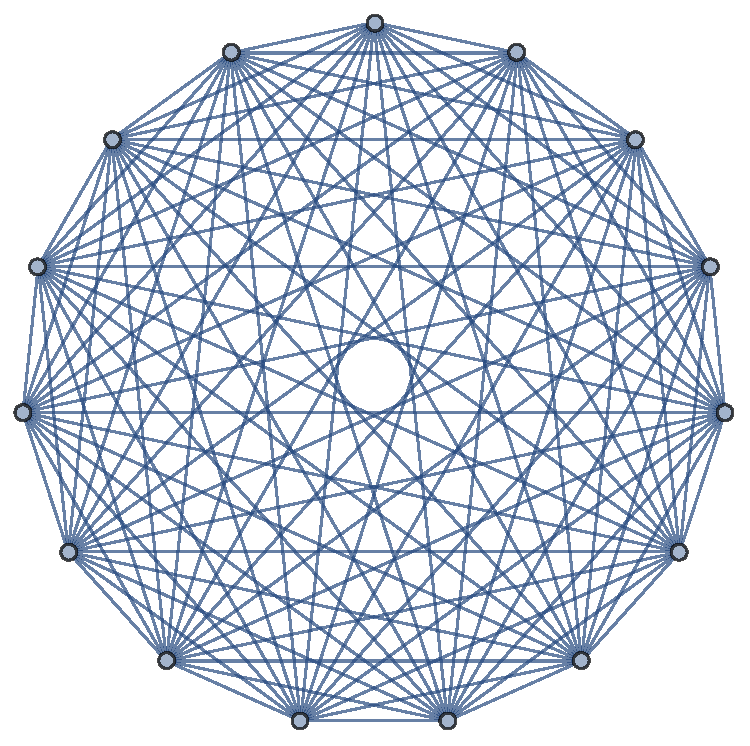
\includegraphics[width=0.7\columnwidth]{K_15}
\caption{The 15-vertex complete graph, $K_{15}$. Every vertex has an edge to every other, with a total of 105 edges.} \label{fig:complete_graph}
\end{figure}

%
% Lattice
%

\subsection{Lattice}

A lattice graph is simply an \mbox{$n\times m$} lattice of vertices (of any geometry, e.g squares), connecting each vertex to its immediate geometric neighbours. This type of graph is useful when link costs are measured in terms of Euclidean distances, and nodes have nearest neighbour links. An example is shown in Fig.~\ref{fig:lattice}.

\begin{figure}[!htb]
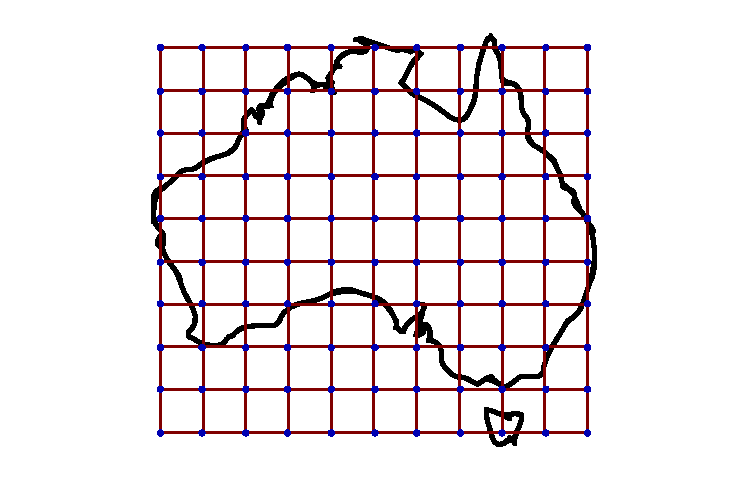
\includegraphics[width=0.7\columnwidth]{lattice}
\caption{A \mbox{$10\times 11$} square lattice graph, and how it might represent a network topology with geographically associated costs. Notice that Hobart has no internet connection (why even include Tasmania at all?).} \label{fig:lattice}
\end{figure}

A slightly distorted lattice graph, in which vertices have been dragged around geometrically to match, for example, cities within a country, closely resembles the topology of the network. Similarly, if the nodes represent houses in the street layout of a highly regular city like Manhattan, a lattice may be a good approximation.

In the case of a balanced lattice, in which all edges are of equal weight, the cost of a route is the sum of the number of steps in the vertical, and number of steps in the horizontal directions, also known as the Manhattan, or $L_1$ distance,
\begin{align}
L_1 = |x_\mathrm{start} - x_\mathrm{finish}| + |y_\mathrm{start} - y_\mathrm{finish}|.
\end{align}
In this case, route finding is simplified, since \emph{all} routes, which strictly traverse in one direction vertically and one direction horizontally, are optimal and of equal distance.

%
% Tree
%

\subsection{Tree} \label{sec:tree_graph}

A tree is a graph containing no cycles, only \emph{branches}. There are many uses for tree graphs, but one property is of particular convenience in many applications: because the graph is acyclic, there is always exactly one path from any vertex to any other. This mitigates the need for shortest-path algorithms designed for general graphs, and simplifies route-finding algorithms (to be discussed in Sec.~\ref{sec:path_exp}).

Trees are specified entirely by \emph{branching parameters} ($b_i$) -- the number of child nodes emanating from a given node, $i$. In general, branching parameters may be distinct for each node, although often trees with symmetries in their branching structures are considered, such as the balanced trees discussed in Sec.~\ref{sec:bal_tree}. A node terminates a branch if its branching parameter is zero (i.e it has no children). The \emph{depth} ($d$) of a tree is the maximum number of steps from the root node to a terminating node with no children. The depth scales between \mbox{$d=|V|$}, for the trivial linear tree (\mbox{$b_i=1$}), and \mbox{$d=O(\mathrm{log}|V|)$} for non-trivial branching parameters (i.e \mbox{$b_i\neq 1$}). The worst-case number of edges that must be traversed to reach any vertex from any other is twice the depth, which implies that cost metrics scale as at most \mbox{$c=O(\mathrm{log}|V|)$}. Trees are the most frugal graphs in their number of edges, which are fixed at \mbox{$|E|=|V|-1$}, irrespective of the branching parameters, since because the graph is strictly acyclic, every addition of an edge requires the addition of a single vertex.

%
% Balanced Tree
%

\subsubsection{Balanced tree} \label{sec:bal_tree}

A balanced tree is a tree with a regular, self-similar structure, in which every node (up to a given depth) is the parent of the same number of sub-nodes, all separated by the same, but equal or smaller edge weights. That is, the network has a hierarchical structure, dividing into sub-networks of decreasing size. Such a network is characterised by just two parameters -- the branching parameter, $b$, and the depth, $d$. Some examples of balanced trees with different $b$ and $d$ are shown in Fig.~\ref{fig:tree_example}.

\begin{figure}[!htb]
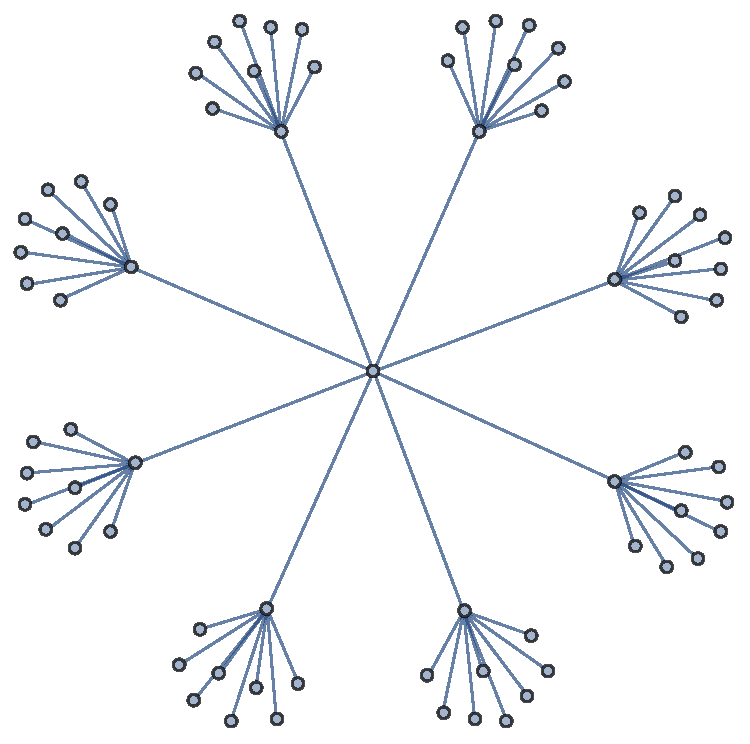
\includegraphics[width=0.75\columnwidth]{tree_3_8} \\
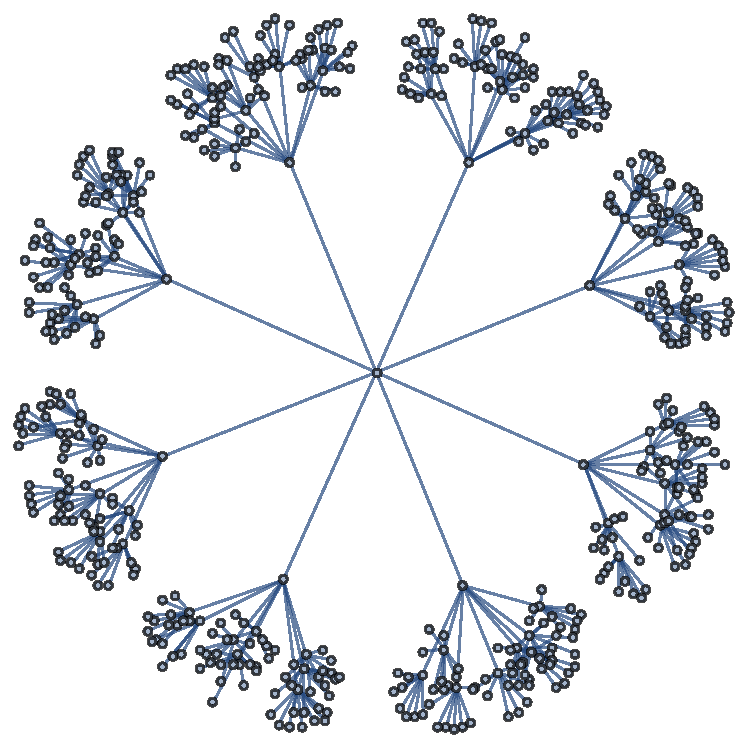
\includegraphics[width=0.75\columnwidth]{tree_4_8} \\
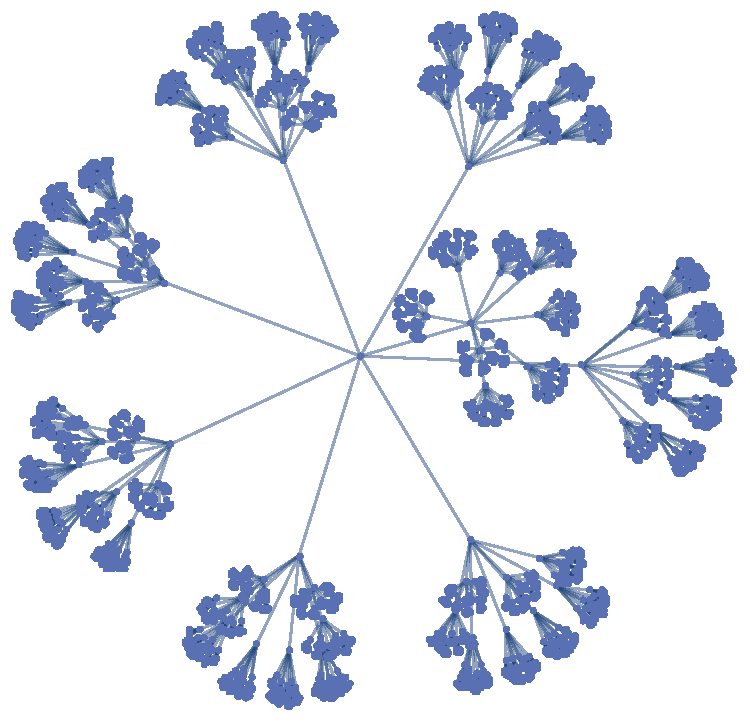
\includegraphics[width=0.75\columnwidth]{tree_5_8}
\caption{Balanced tree graphs with branching factor $b=8$, and depths $d=3,4,5$ (top to bottom). Despite having no redundant paths, the hierarchical structure of balanced trees somewhat resembles that of real-world networks, which are typically decomposed into a pyramid scheme of progressively smaller sub-networks.} \label{fig:tree_example}
\end{figure}

This type of structure is natural in many realistic scenarios. Consider for example a network containing a hierarchy of clusters of nodes representing a LAN, followed by a neighbouring internet router, followed by a city-wide router, followed by a country-wide router. In such a case, this type of general structure is typical.

%
% Random Tree
%

\subsubsection{Random tree}

While balanced trees accurately capture the hierarchical nature of realistic networks, they are somewhat contrived in their perfect symmetry. The sub-networks in a given network are not likely to actually all be identical. Random trees are perhaps more realistic, in that their tree structure captures the hierarchical nature of real-world networks, and also their highly ad hoc nature.

To construct a random tree we simply randomly choose a branching parameter, up to some maximum, for every node. When a node has \mbox{$b_i=0$}, it terminates the lineage. Some examples of random trees are shown in Fig.~\ref{fig:random_tree}.

\begin{figure}[!htb]
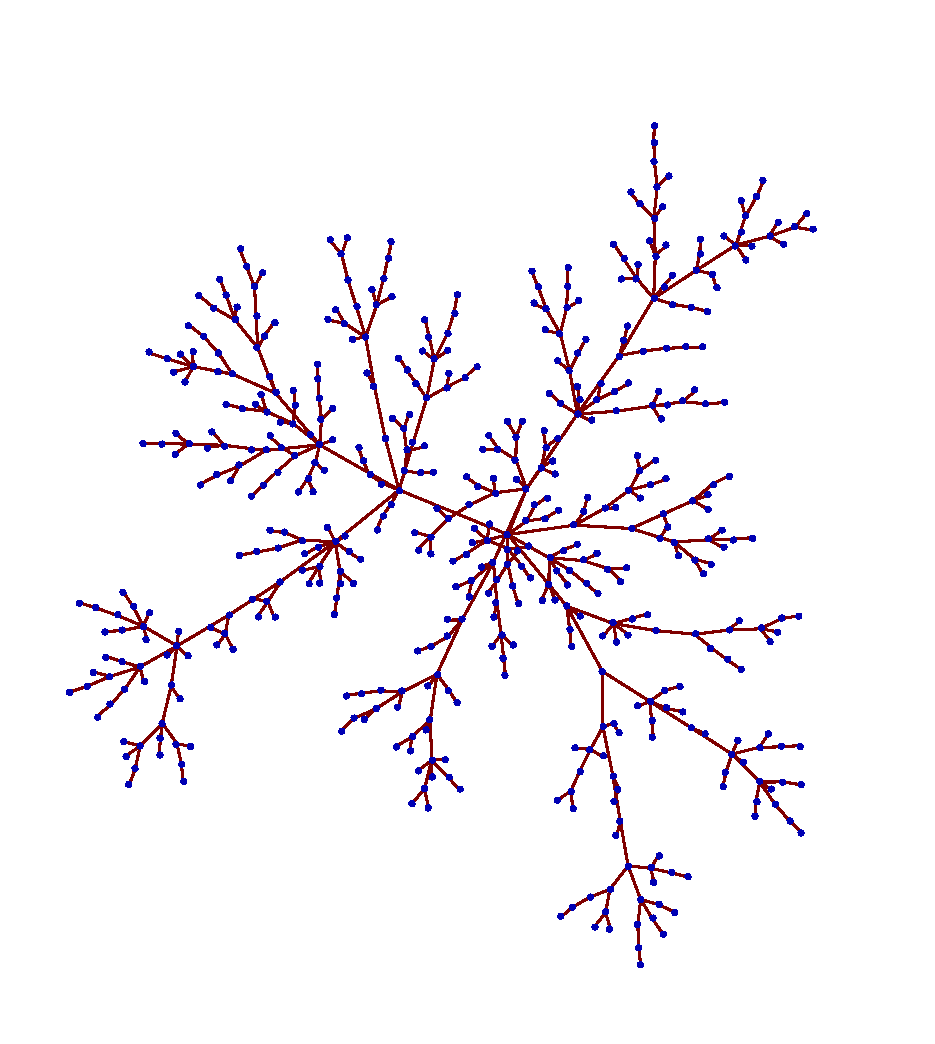
\includegraphics[width=\columnwidth]{random_tree_1} \\
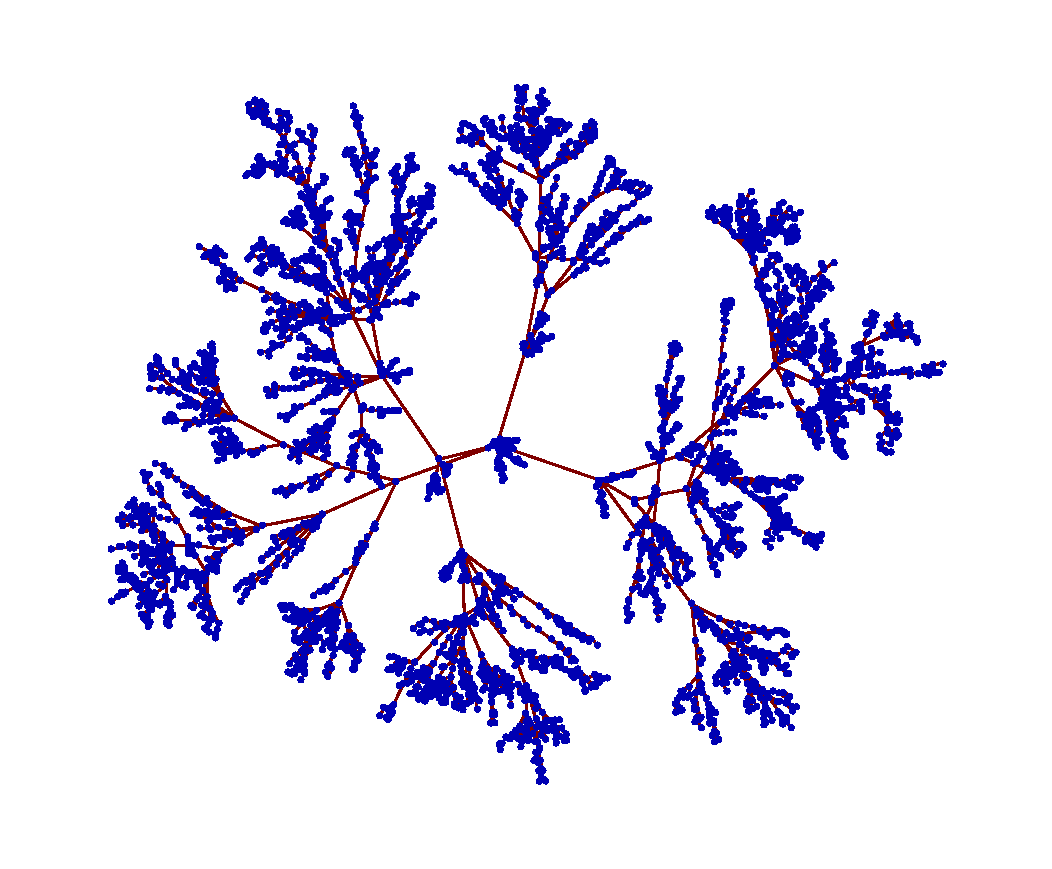
\includegraphics[width=\columnwidth]{random_tree_2}
\caption{Random trees with different randomised branching parameters (higher $b$ at bottom). When a node has zero branches, it terminates the branch. This type of graph topology qualitatively captures the hierarchical, yet ad hoc qualities of many real-world networks, and may act as a useful test model for simulations.} \label{fig:random_tree}
\end{figure}

%
% Minimum Spanning Tree
%

\subsubsection{Minimum spanning tree} \label{sec:graph_MST}

A \emph{spanning tree} $S$, of a graph $G$, is a tree subgraph \mbox{$S\subset G$}, containing every vertex of $G$. The \emph{weight} of a spanning tree is the sum of all its constituent edge weights. Thus, the \emph{minimum spanning tree} (MST) is a spanning tree that minimises weight. An example is shown in Fig.~\ref{fig:mst}. See Sec.~\ref{sec:min_tree} for a discussion on MST algorithms.

\begin{figure}[!htb]
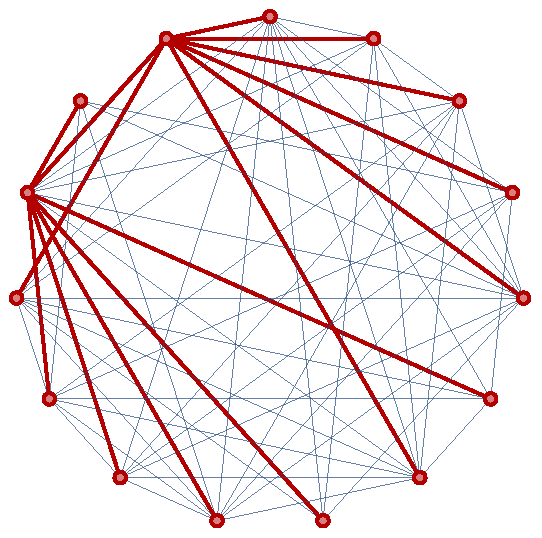
\includegraphics[width=0.8\columnwidth]{mst}
\caption{A random graph (blue) with its MST highlighted (red).} \label{fig:mst}
\end{figure}

The calculation of MST's is most likely to come into consideration when actually performing the initial construction of networks, where we wish to connect all nodes in the network, but using the most frugal possible physical resources. MST's serve this purpose, and since they are trees, inherit all the same properties of tree networks.

%
% Random
%

\subsection{Random}

A variation on the complete graph, $K_{|V|}$, is to instead have a randomised implementation of it, whereby each of the possible edges in $K_{|V|}$ occurs with probability \mbox{$0\leq p_\mathrm{edge}\leq 1$}. We would thereby be able to tune between the complete graph and the completely disconnected graph, representing a randomly connected network with arbitrary average connectivity. Specifically, the average number of links emanating from any node is \mbox{$e_\mathrm{av} = (|V|-1)p_\mathrm{edge}$}. Note that random graphs might be disjoint, making them inappropriate for many networking applications. For asymptotically large random graphs, \emph{percolation theory} \cite{???} provides thresholds for $p_\mathrm{edge}$ such that they remain connected \cite{???}. Fig.~\ref{fig:random_graph} illustrates several graphs with different edge connectivity probabilities.

\begin{figure}[!htb]
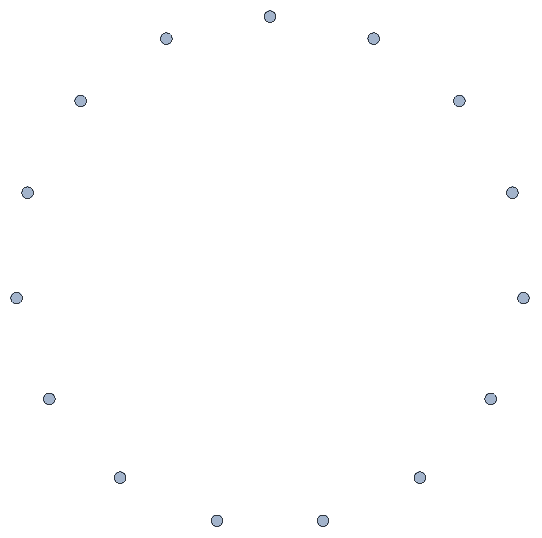
\includegraphics[width=0.6\columnwidth]{random_0}
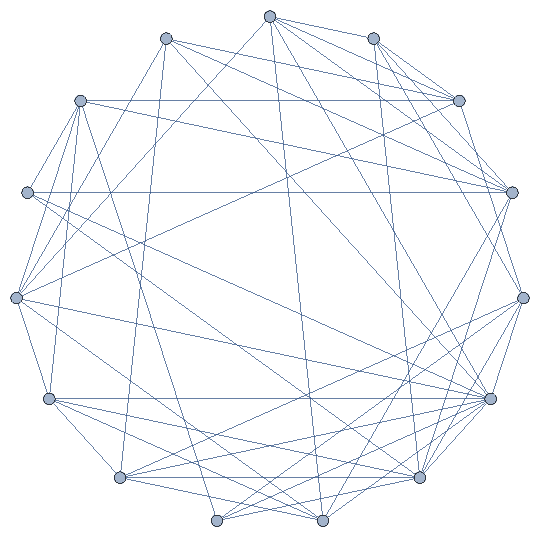
\includegraphics[width=0.6\columnwidth]{random_05}
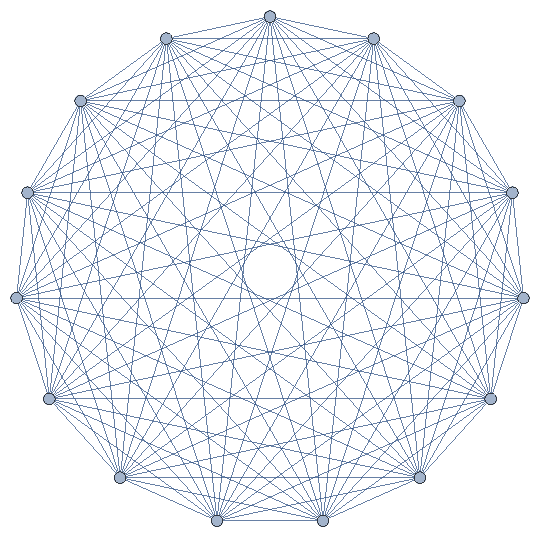
\includegraphics[width=0.6\columnwidth]{random_1}
\caption{The 15-vertex randomly-connected graph. This is the same as $K_{15}$ in Fig.~\ref{fig:complete_graph}, but where edges are present with probabilities \mbox{$p_\mathrm{edge}=0,0.5,1$} (top to bottom).} \label{fig:random_graph}
\end{figure}

Random graphs capture the ad hoc nature of networks that exhibit no planned structure, but are rather cobbled together in a completely improvised manner.

%
% Hybrid
%

\subsection{Hybrid}

Real networks are highly unlikely to fit the exact form factor of any of the classes of graphs presented above. Rather, a truly global internet is inevitably going to comprise many subnetworks, each structured completely independently of one another, with little consistency or large-scale planning between them. Who thinks about the broader structure of the global internet when setting up their office network?

For example, at the global scale, it is entirely plausible that the internet might take on a random tree-like structure. But when we get down to a lower level, the tree structure vanishes and is replaced by all manner of different network topologies, run and maintained by different organisations in their own distinct ways.

Furthermore, the real-world internet is not simply a hierarchy of different types of well-known graph structures. Rather, it takes the form of `glued' graphs, whereby networks running over different mediums, or via different operators, each exhibit their own independent graph topologies, meeting at interconnect points that join the different networks. Typically this yields redundancy in the routes between different nodes.

This hybrid network topology is the norm today in our classical internet, and it is entirely foreseeable that a similar trend will emerge in the future quantum internet as quantum technologies become more mainstream, their networking less well structured, and competing, redundant links are in place.

%
% The Internet Webgraph
%

\subsection{The internet webgraph}

Of course, all the topological structures described until now are in-principle constructs. Of most relevance is the \emph{Webgraph}, the graph of the actual internet. Fig.~\ref{fig:webgraph} illustrates some example webgraphs. The combination of random, densely and sparsely connected, and tree structures, and its clear hierarchy are all evident. This encourages our intuition of the different types of structures present in realistic networks.

\begin{figure}[!htb]
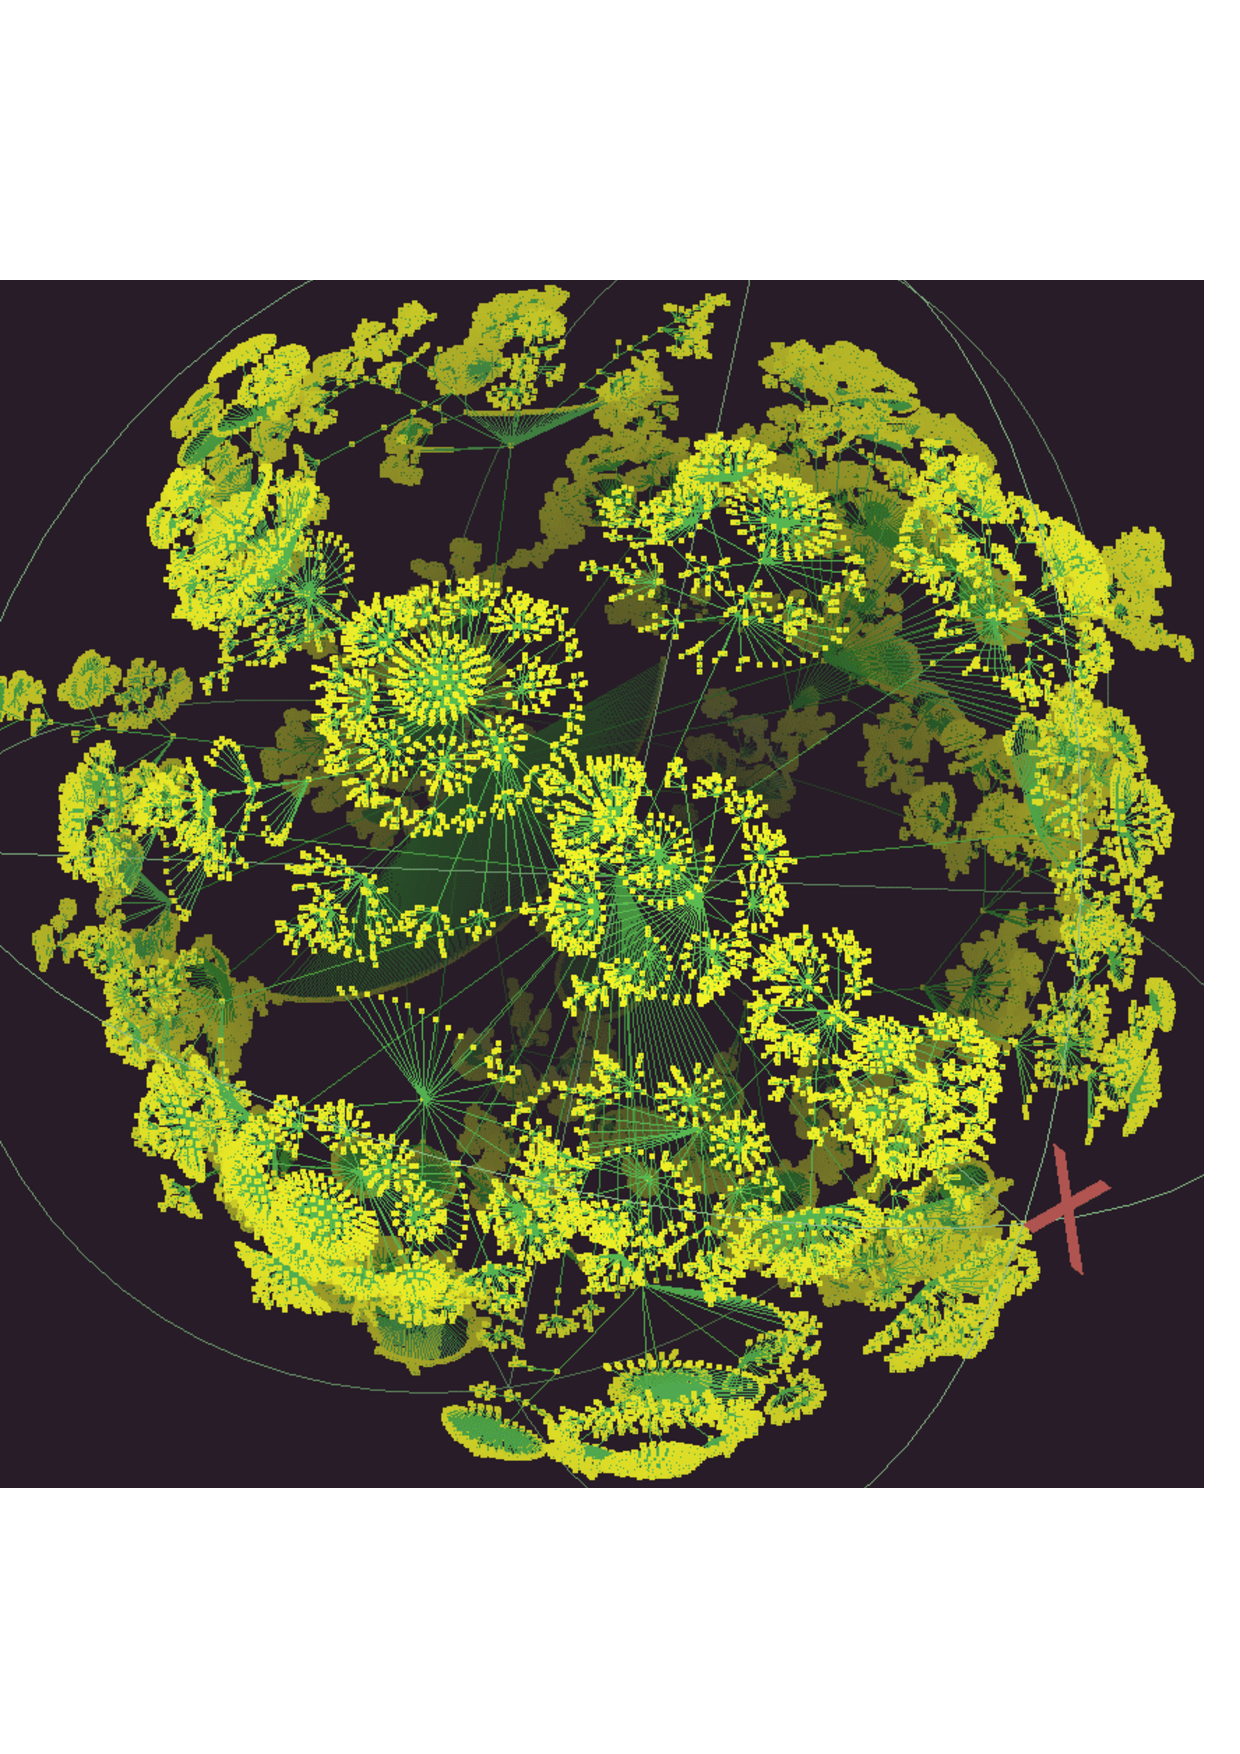
\includegraphics[width=\columnwidth]{webgraph_1} \\
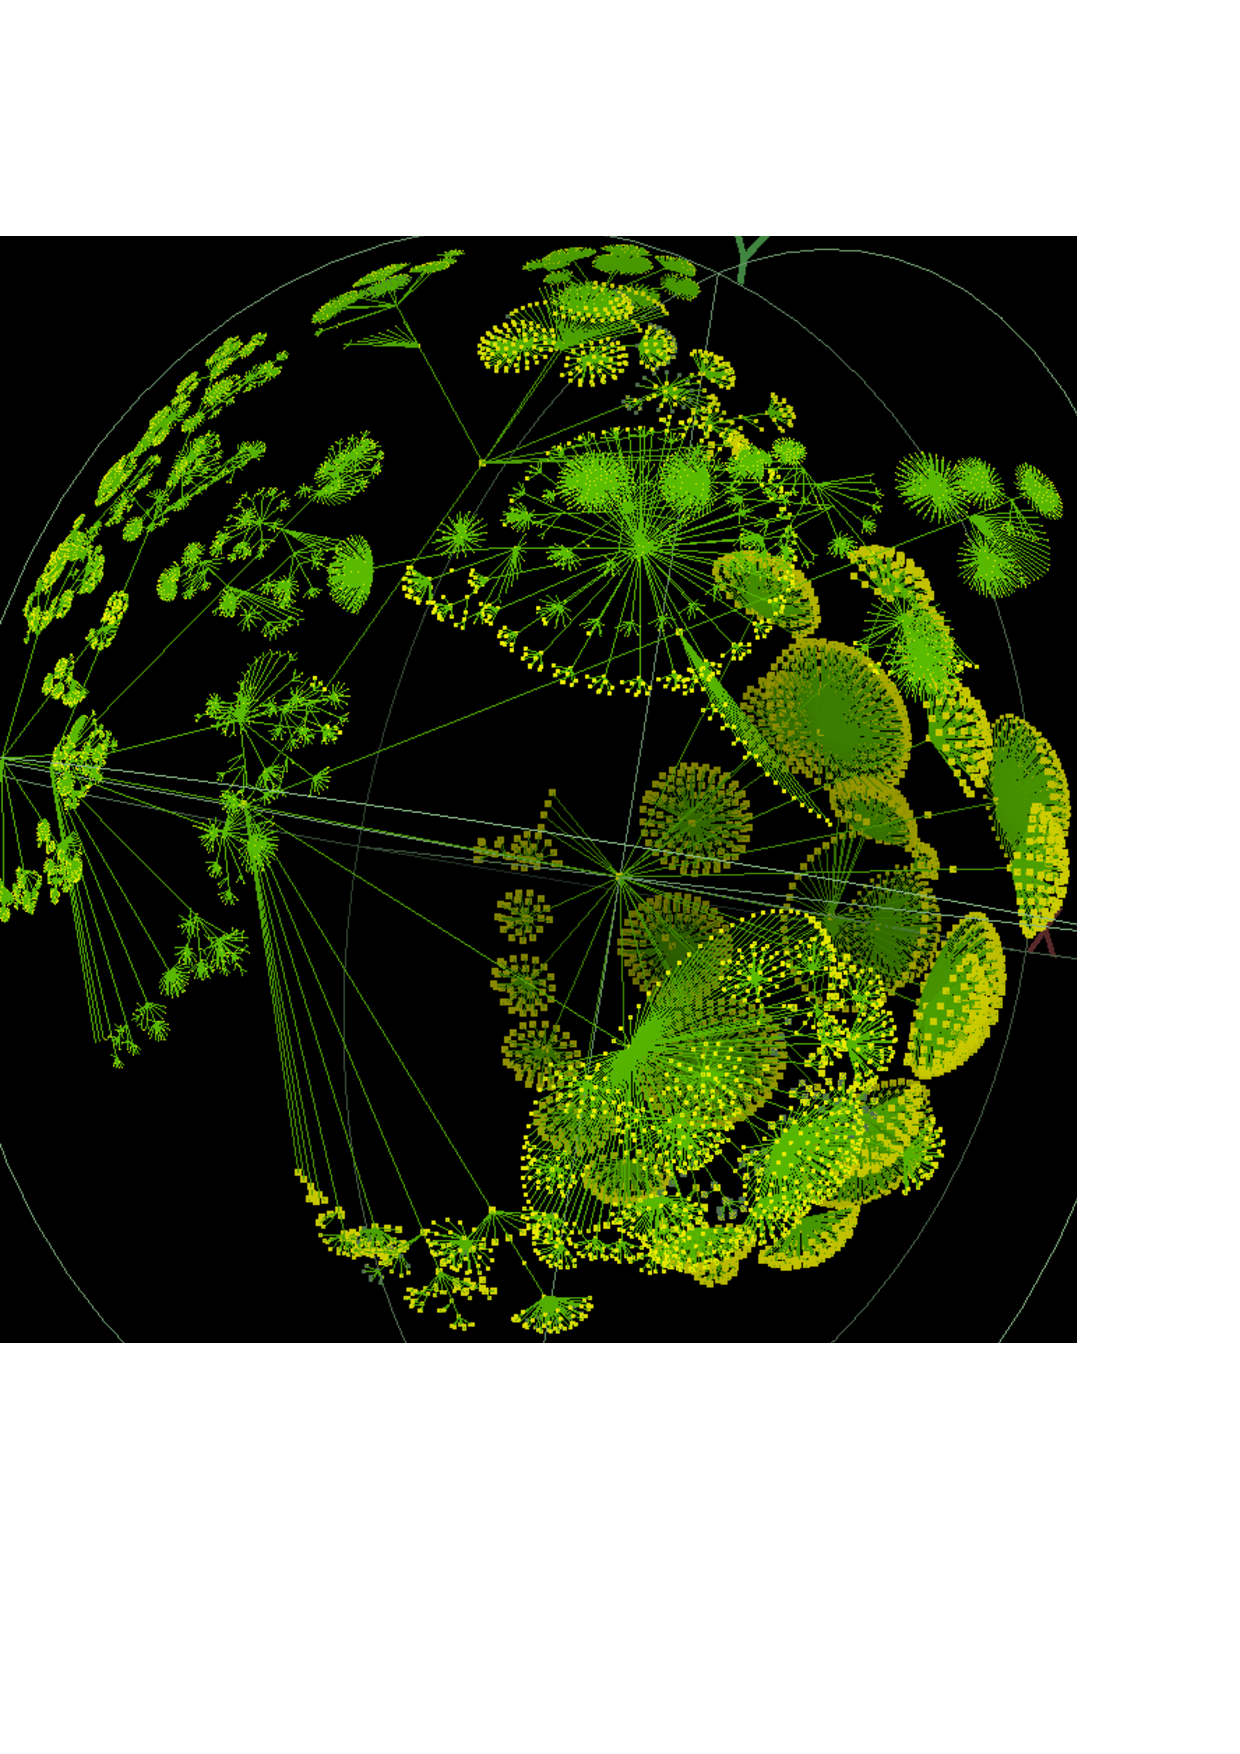
\includegraphics[width=\columnwidth]{webgraph_2}
\caption{Examples of real-world webgraphs, capturing their high-level random tree-like structure. Graphics attributed to the Center for Applied Internet Data Analysis (CAIDA), {\tt \href{http://www.caida.org}{http://www.caida.org}}.} \label{fig:webgraph}
\end{figure}

%
% Scale-Free Networks
%

\subsection{Scale-free networks}

\comment{To do}

%
% Network Algorithms
%

\section{Network algorithms} \label{sec:graph_theory}

Having introduced some of the more relevant graph structures, we now introduce some of the key graph theory algorithms that are of direct relevance to networking theory \cite{bib:RivestAlgBook}. In graph theory, many fundamental problems are believed to be computationally hard to solve. However, there are several important graph algorithms that are classically efficient to solve, and which are of great utility to us as network architects.

%
% Network Exploration & Pathfinding
%

\subsection{Network exploration \& pathfinding} \label{sec:path_exp}

Here the goal is to systematically explore every vertex in an unknown graph exactly once, so as to reconstruct the entire network graph, or to find a target node with unknown location (which can obviously be achieved if the former can be). The two main approaches are \emph{breadth-first-search} (BFS) and \emph{depth-first-search} (DFS) algorithms. In both cases we begin at a starting (root) node, from which we wish to explore the entire graph by only following edges one at a time.

In BFS we proceed from the root node to visit every one of its neighbours. Having done so, and created a list of those neighbours, we proceed onto the neighbours of the neighbours, and so on, until every vertex in the graph has been visited, or the target node found.

In DFS, on the other hand, we begin by following a single arbitrary path until we reach a dead-end, at which point we backtrack until we reach a branch leading to a vertex we hadn't previously visited.

Examples of these two algorithms are shown in Fig.~\ref{fig:BFS_DFS}.

\begin{figure}[!htb]
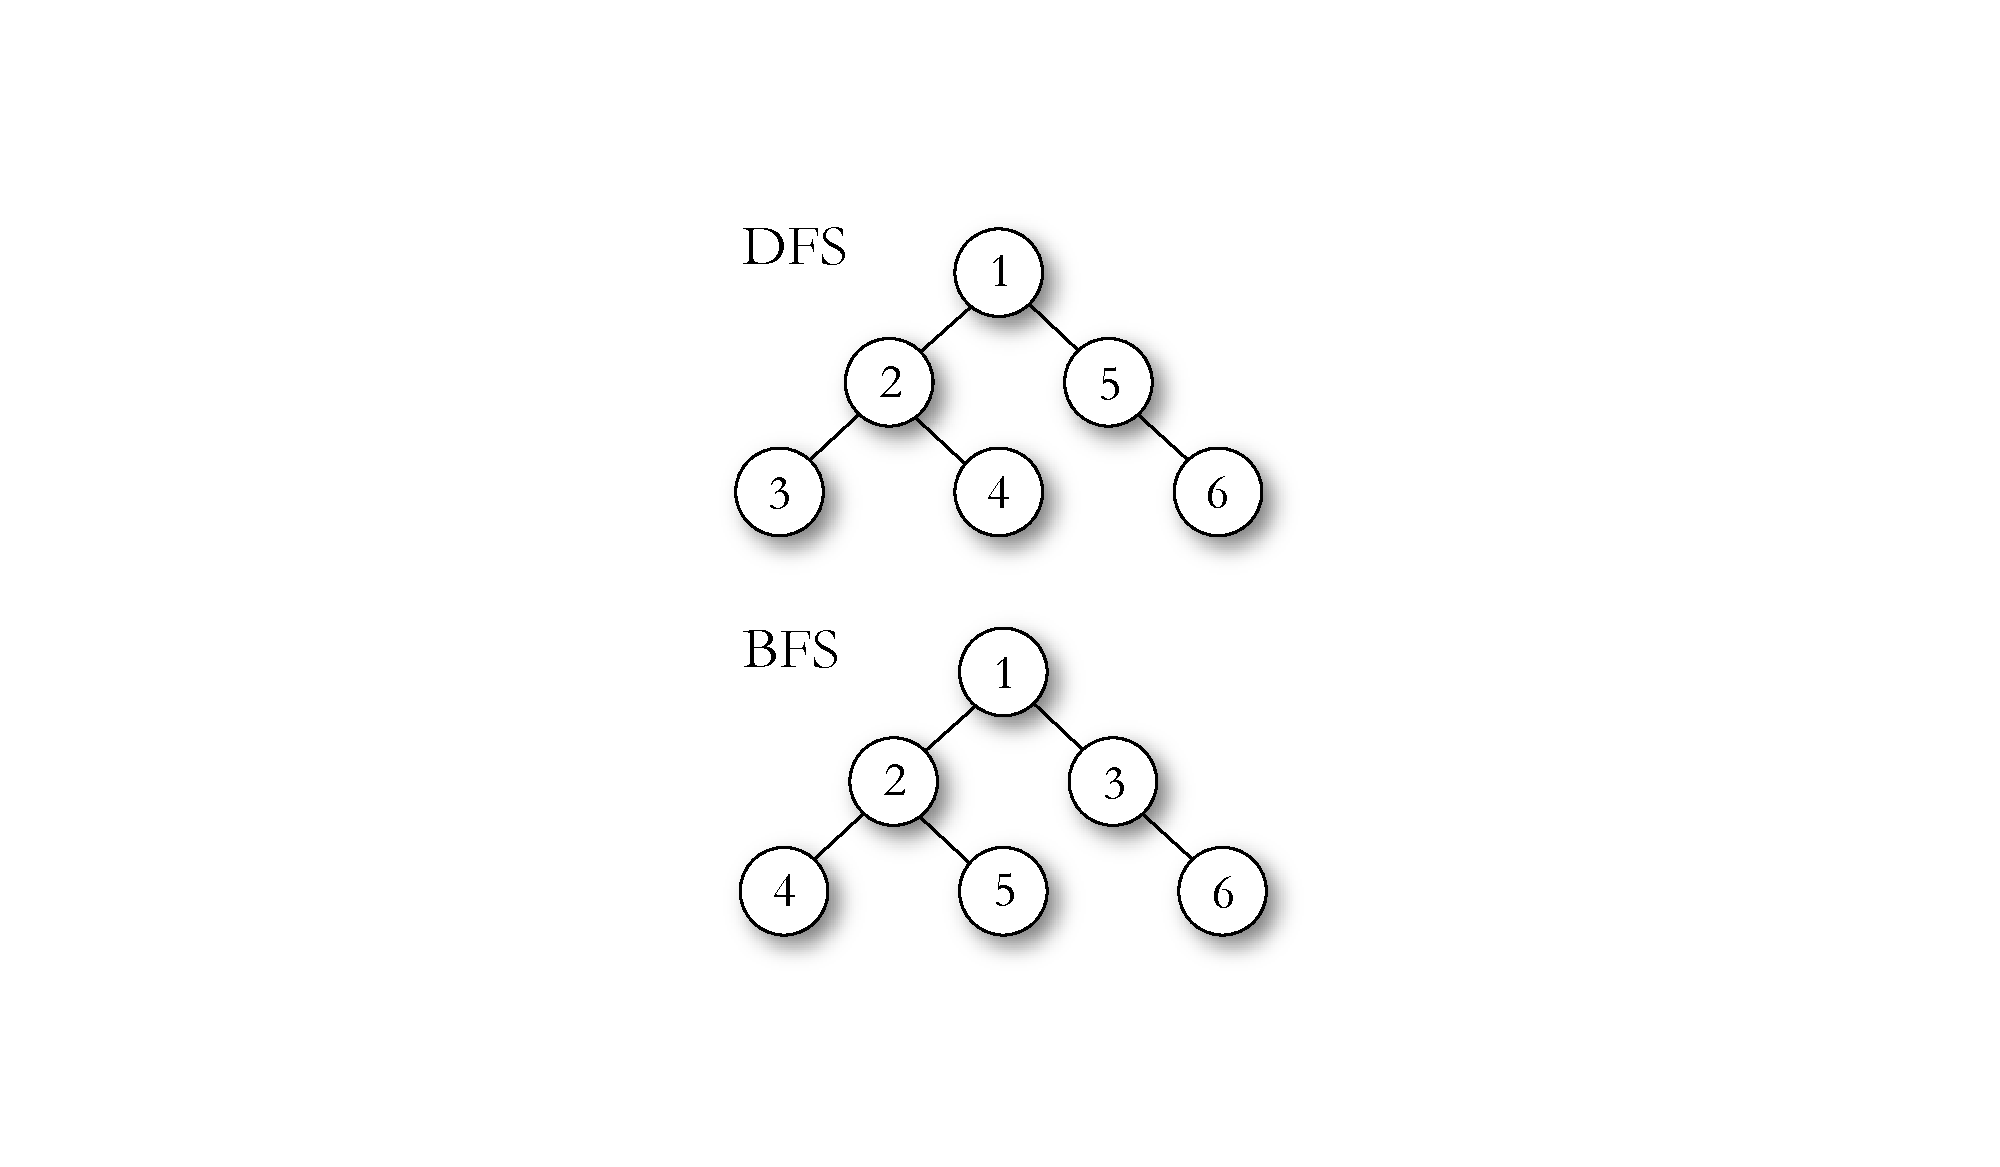
\includegraphics[width=0.6\columnwidth]{BFS_DFS}
\caption{Comparison of the order in which vertices are explored, using the breadth-first-search (BFS) and depth-first-search (DFS) algorithms, where vertex 1 is the root vertex.} \label{fig:BFS_DFS}
\end{figure}

Both BFS and DFS guarantee visiting every vertex in a connected graph, and do so using only nearest neighbour transitions. Such algorithms are therefore very useful for network discovery.

The BFS algorithm is particularly applicable to pathfinding in ad hoc networks. Consider the situation where there is no central authority with full knowledge of the network, overseeing network operation. Rather, everyone needs to figure things out for themselves by only interrogating their neighbours, to whom they have direct connections. This directly leads to a BFS algorithm, where a node speaks to each of its neighbours in turn, who subsequently do the same thing. This can be naturally parallelised, as each node can be interrogating its neighbours independently, thereby implementing a distributed BFS algorithm. Note that, when searching for a target node, while the BFS algorithm obviously finds the target using the smallest number of hops (i.e a lowest-order route), it needn't necessarily find the route with the lowest cost (which is distinct from the number of hops in general). Shortest-path algorithms require a priori knowledge of the full network graph, discussed in Sec.~\ref{sec:shortest_path}.

Both BFS and DFS exhibit runtime \mbox{$O(|V|+|E|)$}, where $|V|$ and $|E|$ are the number of vertices and edges respectively. Thus, these graph exploration algorithms reside in the complexity class \textbf{P}, and are classically efficient.

%
% Shortest-Path
%

\subsection{Shortest-path} \label{sec:shortest_path}

In graph theory, the shortest-path problem is that of finding a subgraph of a given graph $G$, connecting two vertices, \mbox{$A\to B \subset G$}, such that the sum of its edge weights is minimised. In the context of our application to route-finding, this amounts to finding a route that minimises cost.

The first proven shortest-path algorithm was by Dijkstra \cite{bib:Dijkstra59}, which requires runtime $O(|V|^2)$, also residing in \textbf{P}. Subsequently, a number of improvements and variations on Dijkstra's algorithm have been proposed, most notably the $A^*$ algorithm, which has found widespread modern use.

Formally, let $\vec{R}$ be the set of all routes \mbox{$A\to B$}. Then,
\begin{align}
c_\mathrm{opt} = \min_{r\in R} \left(\sum_{i\in r} c_\mathrm{net}(i) \right),
\end{align}
where \mbox{$i\in r$} denotes the $i$th edge in the route $r$.

Fig.~\ref{fig:simp_route_opt} illustrates a directed, edge-weighted graph. A shortest-path algorithm applied between vertices $A$ and $B$ would return \mbox{$R_\mathrm{shortest} = A\to F\to B$} as the minimum cost route.

When introducing network graphs earlier, we insisted upon all costs being associated with edges rather than vertices, and presented a trivial means by which to convert vertex costs to edge costs in Fig.~ \ref{fig:remove_nodes}. This adamance arose because the presently described shortest-path algorithms operate in terms of purely edge weights, not vertex weights. But the mapping we presented from the latter to the former obviates this issue.

This is the motivating factor behind representing network graphs purely in terms of edge weights (Sec.~\ref{sec:quant_proc_in}), thereby enabling compatibility with the shortest-path algorithms.

For the purposes of the QTCP protocol, we are interested in the case of directed graphs (recall that in terms of cost metrics, undirected graphs can be converted to directed graphs by replacing undirected edges with a pair of edges in opposite directions).

Shortest-path techniques find widespread application in many areas. Computer networks are an obvious candidate, since networks are inherently graph-theoretic by nature.

To implement the shortest-path algorithms discussed above, the party performing the calculation requires knowledge of the full network graph. In an ad hoc network, where users might be added to or removed from the network arbitrarily, this isn't necessarily the case.

One solution is for a central authority to be responsible for maintaining a ledger of all network participants and their connectivity, which users are required to notify upon joining or leaving the network. The central authority may then apply shortest-path calculations, which may be queried by users. However, a disruption in connection to the central authority, or failure of nodes to notify the central authority upon joining or leaving the network, introduces a point of failure into the operation of the protocol.

Another approach, which does not require a reliable central authority, is for users to implement network exploration algorithms each time they wish to perform a shortest-path calculation. This facilitates truly ad hoc networking, but incurs the cost overhead associated with nodes frequently implementing network exploration. However, network exploration is a purely classical algorithm, which may run entirely over the classical network, and therefore incurs no cost in quantum resources.

With this approach, a new node can join the network, without having to know anything about the topology of the network. Similarly, upon leaving the network, it needn't notify anyone, since a future interrogation by a neighbour will be detected as a non-existent node. The BFS is therefore highly suited to ad hoc operation.

%
% Single-Source Shortest-Path
%

\subsection{Single-source shortest-path} \label{sec:single_source_sp}

The shortest-path algorithm by Dijkstra presented above finds the shortest route between two specified nodes in a network. However, when employing {\sc Individual} routing strategies, where there is no central mediation of the network, each node desires an up-to-date routing table, showing the best route to take to any other point in the network. Then, upon receiving packets with particular destinations, rather than repeatedly applying Dijkstra's algorithm, we can simply look up the destination on the node's local routing table.

Single-source shortest-path algorithms address this problem by calculating the shortest paths from the current node to \emph{every} other node in the network topology.

The best-known algorithm for this problem is the Bellman-Ford (or Bellman�Ford�Moore) algorithm \cite{BF}, which requires worst-case runtime of $O(|V|\cdot |E|)$. Clearly this is more complex than Dijkstra's algorithm for finding a particular shortest-path. But it is more efficient than using brute-force to find the shortest-path between every pair of nodes in the network via repeated application of Dijkstra.

%
% Minimum Spanning Tree
%

\subsection{Minimum spanning tree} \label{sec:min_tree}

MST algorithms find a MST of some arbitrary graph. Like the shortest-path problem, it has a polynomial-time, deterministic algorithm (i.e it resides in \textbf{P}). The first MST algorithm \cite{bib:Boruvka26} required $O(|E|\log |V|)$ runtime. Numerous variations have since been proposed, with little change to the underlying scaling.

Because MST algorithms are efficient, they play a very useful role in the design of real-world network topologies, where resource minimisation is crucial.

Fig.~\ref{fig:mst} shows an example of a graph with its MST.

%
% Minimum Cost Flow
%

\subsection{Minimum cost flow} \label{sec:min_cost_flow_prob}

The \emph{minimum cost flow problem} \cite{???} is that of minimising costs through a network for a specified amount of flow, which acts as a constraint on the problem. The definition of `cost' in this context is compatible with our earlier definition of cost metrics.

This problem can be efficiently solved using linear programming. Specifically, cost metrics along links in series are given by linear combinations of individual link costs. If, in addition, we let our net cost function be linear in the constituent costs then the net cost will also be linear in all the edge weights. This lends itself directly to optimisation via linear programming techniques. Algorithms for linear programming, such as the \emph{simplex} algorithm, have polynomial-time solutions (i.e reside in \textbf{P}), and a plethora of software libraries are available for implementing them numerically.

%
% Maximum Flow
%

\subsection{Maximum flow} \label{sec:max_flow_prob}

The \emph{maximum flow problem} \cite{???} is the seemingly simple goal of -- as the name suggests -- maximising network flow, without consideration for any of the other costs metrics or attributes associated with the network. This type of problem is relevant when brute bandwidth is the dominant goal.

This problem can be tackled using a number of techniques. In some circumstances, linear programming techniques can be employed. The best-known algorithm is the Ford-Fulkerson algorithm \cite{???}, which finds a solution in \mbox{$O(|E|\cdot c_\mathrm{max})$} runtime, where $|E|$ is the number of links in the network and $c_\mathrm{max}$ is the maximum cost present in the network. The algorithm behaves pathologically in some conditions, which can easily be overcome in the context we present here. Using Ford-Fulkerson as a starting point, numerous other more sophisticated algorithms have been developed.

%
% Multi-Commodity Flow
%

\subsection{Multi-commodity flow} \label{sec:multi_comm_flow}

The \emph{multi-commodity flow problem} \cite{???} generalises the previous algorithms to be applicable to multi-user networks. The generalisation is that there may be a number of distinct senders, residing on different nodes, each transmitting to distinct recipients, residing on different nodes. This is the most realistic scenario we are likely to encounter in a real-world quantum internet, where networks will inevitably be shared by many users.

Unfortunately the computational complexity of solving this problem is much harder than the previous algorithms in general. Specifically, solving the problem exactly is \textbf{NP}-complete in general. However, in specific circumstances it can be approached using linear programming or polynomial-time approximation schemes.

Note that, using Grover's search algorithm, although not efficient, quantum computers offer a quadratic improvement in the runtime of \textbf{NP}-complete problems, which is pertinent to consider in the upcoming quantum era.

%
% Protocols for the Quantum Internet
%

\section{Protocols for the quantum internet} \label{sec:protocols_quant_int}

There are countless applications for the long-distance communication and processing of quantum data. We will outline some of the most notable examples. Broadly, we will begin with discussion of \emph{low-level protocols} that form the primitives upon which other protocols are built. We will then progressively move towards \emph{high-level protocols}, culminating with full \emph{cloud quantum computing}.

Much of the recent experimental progress in quantum technology has been in the area of low-level protocols, although demonstrations of higher-level protocols are rapidly accelerating.

We keep in mind that although throughout this presentation we have been very quantum computing-centric, quantum computing is not the \emph{only} quantum resource worth communicating. In the same way that \emph{digital assets} encompass a broad range of digital systems and information, any aspect of a quantum system -- from a state, to an operation, storage, to a measurement, or anything else -- could be treated as a \emph{quantum asset}, which, for generality, we would like our quantum networks to be able to handle.

At the lowest physical level, quantum protocols have in common that they involve state preparation, evolution, and measurement as the fundamental primitives upon which more complex protocols are constructed. We consider these primitive resources in detail, before building upon them to consider some of the major elementary quantum protocols that implement tasks of practical interest. All of those discussed here have been subject to extensive experimental investigation and demonstration.

%
% State Preparation
%

\subsection{State preparation}

The first step in any quantum protocol involves the preparation of some kind of quantum state. Some quantum states are easy and cheap to prepare. Others are complex and costly. Thus, the most fundamental quantum asset that a quantum network must handle is the preparation and communication of quantum states.

A state prepared by Bob and sent to Alice might be prepared in isolation, or it might be entangled with a much larger system held by Charlie, that Alice does not have full access to. In that case, it would be impossible for Alice to prepare the state on her own, unless she were to first establish a relationship with Charlie. Alternately, maybe Alice just isn't very well-resourced, and can't do much on her own. The ability to let someone else prepare her desired quantum states for her would be highly appreciated.

Given the emphasis on quantum optics in quantum networking, it should be noted that optical quantum state engineering has broad applications, but can be very challenging in general. Single-photon state engineering, for example, finds ubiquitous applications in quantum information processing protocols, and has become commonplace. Most notably, linear optics quantum computing (Sec.~\ref{sec:KLM_univ}), and some quantum metrology protocols (Sec.~\ref{sec:metrology}) rely on single-photon state preparation. `Push-button' (i.e on-demand) single-photon sources would be a prized asset to many undergraduate experimentalists, were they able to afford them. But with access to the quantum internet, they could purchase single photons from another better-resourced lab, with QoS constraints guaranteed by QTCP.

The QTCP protocol is ideally suited to facilitating this kind of transaction. With the use of efficiency and purity cost metrics, QoS guarantees could be established for the efficiency and purity of a licensed single-photon source. In the case of single photons, the dephasing metric is irrelevant, since photon-number states are phase-invariant. This is an elegant example of the value of the versatility of having the QTCP protocol track multiple cost metrics for quantum packets, since different metrics will be of relevance to different messages. Were the message a coherent state, $\ket\alpha$, on the other hand, dephasing would be of utmost importance, whereas loss would be less critical, as lossy coherent states remain as coherent states and retain their coherence.

We see that even the most basic primitive in quantum technologies -- state preparation -- already brings with it much to take into consideration when designing quantum networks. However, the QTCP protocols we described earlier are versatile enough to be capable of mediating their distribution across quantum networks, whilst providing QoS guarantees.

%
% Coherent States
%

\subsubsection{Coherent states} \label{sec:coherent_states}

Coherent states (Sec.~\ref{sec:coherent_state_enc}), although not strictly quantum states, nonetheless find broad applications in quantum protocols, for example as the pump for spontaneous parametric down-conversion (SPDC) sources (Sec.~\ref{sec:single_phot_src}), or as a phase-reference for homodyne detection (Sec.~\ref{sec:homodyne}). Coherent states are rather trivial prepare, as they are closely approximated by laser sources. Despite their triviality, high quality lasers can nonetheless become very expensive, large, and inaccessible to the not-so-well-resourced end-user.

%
% Single-photons
%

\subsubsection{Single-photons} \label{sec:single_phot_src}

Single-photon sources (Sec.~\ref{sec:single_phot_enc}) \cite{bib:Oxborrow05} are of particular interest, as a foundational building block in many optical quantum information processing applications, such as linear optics quantum computing (Sec.~\ref{sec:KLM_univ}) and quantum key distribution (Sec.~\ref{sec:QKD}).

The most common approach to preparing single-photon states is via heralded SPDC \cite{bib:URen03, bib:URen05}, whereby a coherent pump source is down-converted into two-mode photon-pairs via a second-order non-linear crystal with interaction Hamiltonian of the form,
\begin{align}
\hat{H}_\mathrm{SPDC} = \xi(\hat{a}_\mathrm{p}\hat{a}_\mathrm{s}^\dag\hat{a}_\mathrm{i}^\dag + \hat{a}_\mathrm{p}^\dag\hat{a}_\mathrm{s}\hat{a}_\mathrm{i}),
\end{align}
where $\hat{a}_\mathrm{p}$, $\hat{a}_\mathrm{s}$ and $\hat{a}_\mathrm{i}$ are the photonic annihilation operators for the pump (input), and \emph{signal} and \emph{idler} (output) modes respectively. This has the clear intuitive interpretation as the coherent exchange of photon-pairs in the output modes with photons in the coherent pump.

Specifically, a two-mode SPDC state takes the form,
\begin{align}
\ket\psi_\mathrm{SPDC} = \sqrt{1-\chi} \sum_{n=0}^\infty \chi^n \ket{n,n},
\end{align}
where $\chi$ is the squeezing parameter, a function of the pump-power and properties of the crystal. Applying the single-photon projector, \mbox{$\ket{1}\bra{1}$}, to the first mode yields the single-photon state in the other, up to normalisation, which reflects the inherent non-determinism. The preparation success probability is derived from the amplitude of the \mbox{$n=1$} term as,
\begin{align}
P_\mathrm{prep}=\chi^2(1-\chi),
\end{align}
assuming ideal photo-detection. Thus, the perfect photon-number correlation enables heralded preparation of states with exactly one photon in principle.

This description is purely in the photon-number basis. However, as discussed in Sec.~\ref{sec:spatio_temporal}, photons also have spatio-temporal characteristics. This strongly affects state preparation when using heralded SPDC, particularly state purity, and much effort has been invested into engineering the spectral structure of SPDC states so as to maximise purity and indistinguishability \cite{bib:Aichele02, bib:Branning00}.

This process is relatively cheap, and widely used, but nonetheless might be out of reach for many end-users. SPDC is is quickly being superseded by superior technologies in cutting-edge labs, such as quantum dot sources, which have deterministic, push-button potential \cite{bib:Santori01, bib:Kiraz04}. Techniques based on cavity quantum electrodynamics (QED) \cite{bib:Brattke01} and molecular fluorescence \cite{bib:Brunel99} have also been demonstrated. However, such sources are very much in their developmental stages, and relatively expensive.

Generally speaking, a push-button photon source could be constructed from any two-level system, comprising a ground state ($\ket{g}$) and an excited state ($\ket{e}$) with short lifetime, whereby relaxation via the \mbox{$\ket{e}\to\ket{g}$} transition emits a photon. Then, pumping the system to excite it to the $\ket{e}$ state, and waiting for spontaneous decay yields a single photon.

%
% NOON States
%

\subsubsection{NOON states} \label{sec:NOON}

So-called NOON states, path-number entangled two-mode states of the form,
\begin{align}
\ket\psi_\mathrm{NOON} = \frac{1}{\sqrt{2}}(\ket{N,0}+\ket{0,N}),
\end{align}
may be exploited to perform Heisenberg-limited quantum metrology, allowing extremely precise phase measurement with large photon-number $N$ \cite{bib:Dowling08}. However, these states are notoriously difficult and technologically challenging to prepare, and can only be prepared non-deterministically using linear optics \cite{bib:Cable07}.

If a remote server had the capacity to prepare such states, they would be in high demand across the globe. Hindering this, NOON states are very fragile creatures. First, they exhibit exponentially increased susceptibility to loss -- loss of just a single photon completely decoheres the state, rendering it useless for metrological purposes. Second, the large photon-number, $N$, amplifies dephasing by a factor of $N$, as discussed in Sec.~\ref{sec:dephasing_error}. These considerations can be readily accommodated for in the QTCP protocol by tracking dephasing and loss metrics of the packets encapsulating the NOON states.

%
% Cluster States
%

\subsubsection{Cluster states}

In addition to the simple single- or two-mode states discussed above, an entire universal quantum computation can be performed using the `cluster state' measurement-based model for quantum computation (Sec.~\ref{sec:CSQC}). Here state preparation can not only be outsourced, but distributed, with different hosts preparing different parts of the state, which are then `stitched together'.

The beauty of this type of state is that there is a natural separation between state preparation and computation, with the preparation state being far more technologically challenging than the computation stage. Thus, Alice might ask better-resourced Bob to prepare a cluster state and send it to her, at which point she implements the computation herself using simple single-qubit measurement operations.

%
% Greenberger-Horne-Zeilinger States
%

\subsubsection{Greenberger-Horne-Zeilinger states}

Another class of states is Greenberger-Horne-Zeilinger (GHZ) states \cite{bib:GHZ89}, which are maximally-entangled states across an arbitrary number of qubits, of the form,
\begin{align}
\ket\psi_\mathrm{GHZ} = \frac{1}{\sqrt{2}}(\ket{0,\dots,0} + \ket{1,\dots,1}).
\end{align}

GHZ states are useful for various quantum information processing applications, including quantum anonymous broadcasting (Sec.~\ref{sec:anon_broad}). These states are particularly susceptible to loss, since the loss of a single qubit completely decoheres the state into a perfect mixture of the \mbox{$\ket{0,\dots,0}$} and \mbox{$\ket{1,\dots,1}$} states, with complete loss of entanglement and coherence.

%
% Bell States
%

\subsubsection{Bell states} \label{sec:bell_state_res}

Bell states (Eq.~\ref{eq:bell_basis}), also known as Einstein-Podolsky-Rosen (EPR) pairs \cite{bib:EPR35}, which are maximally-entangled two-qubit states, are particularly useful for many applications, including quantum teleportation (Sec.~\ref{sec:teleport}), cluster state preparation (Sec.~\ref{sec:CSQC}), and entanglement swapping (Sec.~\ref{sec:swapping}). Bell states are the special case of two-qubit cluster states, or equivalently, two-qubit GHZ states. They may be directly prepared as the two-mode output from a type-II (\comment{Type-I or type-II???}) SPDC source, or using non-deterministic linear optics from single-photon sources.

There are four Bell states, defined as, 
\begin{align} \label{eq:bell_basis}
\ket{\Phi^{\pm}} &= \frac{1}{\sqrt{2}} (\ket{0}_A\ket{0}_B \pm \ket{1}_A\ket{1}_B), \nonumber \\
\ket{\Psi^{\pm}} &= \frac{1}{\sqrt{2}} (\ket{0}_A\ket{1}_B \pm \ket{1}_A\ket{0}_B),
\end{align}
which are locally equivalent to one another via the application of Pauli operators, and may therefore be transformed to one another without classical or quantum communication between the two parties.

%
% Cat States
%

\subsubsection{Cat states}

Cat states (Sec.~\ref{sec:cat_enc}) are extremely difficult to prepare, most easily via non-linear processes. However, they are very useful for optical quantum computation and for the study of macroscopic quantum systems, when using large coherent amplitudes. Because of the difficulty of their preparation, the ability to outsource it would be very valuable.

%
% Squeezed States
%

\subsubsection{Squeezed states}

Of particular interest to metrology in particular, are squeezed states, states which have been longitudinally distorted in phase-space. In the metrological context, squeezed states enable sub-shotnoise limited metrology \cite{???}, thereby outperforming any classical protocol, using, for example, coherent states or single photons.

Mathematically, squeezing is represented using the squeezing operator,
\begin{align}
\hat{S}(\xi) = \mathrm{exp}\left[ \frac{1}{2}(\xi^*\hat{a}^2 - \xi{\hat{a}^{\dag 2}})\right],
\end{align}
where $\hat{a}$ is the photonic creation operator. Experimentally, such states are prepared using non-linear crystals. It is intuitively obvious that linear optics cannot prepare such states, owing to the non-linear terms in the squeezing operator, which does not preserve photon-number.

Of particular interest are squeezed coherent states, $\hat{S}(\xi) \ket{\alpha}$, which are minimum uncertainty states, saturating the Heisenberg uncertainty principle. 

\comment{To do}

%
% More Exotic States of Light
%

\subsubsection{More exotic states of light}

As discussed in Sec.~\ref{sec:exotic}, many other far more elaborate states are very difficult to prepare, and it would be highly desirable if they could be obtained/purchased over a quantum network. This includes certain CV states, which have utility in alternate models for quantum computing \cite{bib:Menicucci06, Ralph, Lund}, and squeezed states, which can be useful for sub-shotnoise limited metrology \cite{???}.

%
% Matter Qubits
%

\subsubsection{Matter qubits}

In addition to preparing optical states, they can be used to mediate the preparation of systems comprising matter qubits, using which-path erasure techniques (Sec.~\ref{sec:hybrid}, Fig.~\ref{fig:barrett_kok}) or light-matter interactions (Sec.~\ref{sec:opt_inter}, Fig.~\ref{fig:opt_int}). These techniques are very versatile, and apply to many different matter qubit systems, such as two-level atoms, nitrogen-vacancy centres, quantum dots, and atomic ensembles.

This is useful when matter-based architectures are more scalable or technologically simpler than all-optical architectures (Sec.~\ref{sec:KLM_univ}), and particularly for quantum memory (Sec.~\ref{sec:memory}), when using matter qubits with long lifetimes.

%
% Measurement
%

\subsection{Measurement}

As a last (and possibility also intermediate) step in any quantum protocol is the measurement of quantum states. State measurement is, in the most general context, essentially state preparation in reverse, and brings with it many of the same challenges.

Different detection schemes bring with them their own (potentially substantial) costs and technological challenges. State of the art micropillar photo-detectors \cite{???}, at the time of writing, cost on the order of hundreds of thousands of dollars, and require a sophisticated laboratory setup. Clearly this type of infrastructure is inaccessible to many players, and borrowing or licensing access to such equipment over a quantum network would pave the way for broader accessibility to state of the art technology.

Each type of state being measured, in combination with the nature of the detection scheme, brings with it their own limitations. For example, number-resolved photo-detectors exhibit dead-time, are too slow to enable fast-feedforward, have spectral filtering characteristics, and mode-matching requirements. 

These represent significant technological challenges, which are costly to overcome, necessitating outsourcing over the quantum internet to become economically viable on a large scale. However, the QTCP protocol is able to accommodate error metrics and attributes covering all the above error models, enabling reliable, predictable QoS for outsourced quantum measurement.

With the ability to perform measurements over a complete basis for the respective system, QST, and consequently QPT (Sec.~\ref{sec:QPT}), can also be outsourced, as both these protocols are built entirely upon determining measurement expectation values in some known basis.

%
% Photo-detection
%

\subsubsection{Photo-detection} \label{sec:photo_detection}

Perhaps the most useful, and ubiquitous, type of optical state measurement is photo-detection \cite{RohdePDReview}, where we would like to count photon-number. Broadly, there are two main classes of photo-detectors -- \emph{number-resolved} and \emph{non-number-resolved} (or `bucket' detectors). These behave exactly as the names suggest, with the latter typically being more expensive and technologically demanding than the former. The most common form of photo-detection is using is via avalanche photo-detectors, which are cheap but non-number-resolving.

The key parameter of interest in a photo-detector is its efficiency, $\eta$ -- the probability that a given incident photon will trigger the detector. For most applications, the goal is to maximise $\eta$. As one might expect, there is a direct tradeoff between $\eta$ and cost, with very high-efficiency detectors often economically out of reach for many experimentalists.

Mathematically, the measurement operators for number-resolved detection are,
\begin{align}
\hat\Pi_n = \eta^{n} \sum_{m=n}^\infty \binom{m}{n} (1-\eta)^{m-n} \ket{m}\bra{m},
\end{align}
for measurement outcome $n$. And for non-number-resolved detection,
\begin{align}
&\hat\Pi_0 = \sum_{m=0}^\infty (1-\eta)^{m} \ket{m}\bra{m}, \nonumber \\
&\hat\Pi_{>0} = \mathbb{\hat{I}} - \hat\Pi_0.
\end{align}
Thus, inefficiency results in projection onto the wrong photon-number, making measurement outcomes incorrect.

Number-resolved detectors are the more challenging ones to experimentally realise. However, using multiplexing techniques, non-number-resolved detectors can be used to closely approximate number-resolution \cite{bib:Fitch03, bib:Banaszek03, bib:Achilles04, bib:RohdeCompDet07}, at the expense of an overhead in the complexity of the experiment, which comes at a cost. Specifically, there is a direct tradeoff between the confidence in photon-number outcomes, and experimental overhead. The idea behind this is simple. We spread out an $n$-photon state evenly across a large number of modes, $m$, and detect each one independently using a non-number-resolved photo-detector. If \mbox{$m\gg n$}, it is unlikely that more than a single photon will reach any given detector. Thus, by summing the total number of clicks across all detectors, we closely approximate the true photon-number. This multiplexing can be performed in the spatial- or temporal-domains, and has been a widely employed technique in laboratories without access to expensive number-resolved detectors.

In addition to their operation in the photon-number basis, photo-detectors exhibit spatio-temporal characteristics, which affect their operation in quantum information processing protocols \cite{RohdePDReview}. For example, imperfect spectral response can undermine photonic interference, affecting which-path erasure protocols, such as Bell state projection (Sec.~\ref{sec:bell_proj}). However, in many cases this can be improved upon using spectral filtering or time-gating techniques, also at the expense of experimental complexity and resource overhead.

Furthermore, photo-detectors are subject to `dead-time', which renders them inactive for a finite period following a detection event. This is of especial importance in time-bin-encoded schemes (Sec.~\ref{sec:time_bin}), where detectors must resolve photons over very short timescales on the order of nanoseconds.

%
% Homodyning
%

\subsubsection{Homodyning} \label{sec:homodyne}

A homodyne detector interferes a state with a coherent state on a beamsplitter, which acts as a phase-reference, before photo-detecting both output modes. By sweeping through the amplitude and phase of the reference beam, we are able to directly sample points in phase-space, allowing the Wigner function of an unknown state to be fully reconstructed. This measurement technique is typically applied to CV states rather than photon-number states. While conceptually straightforward, preparing the reference beam requires a coherent source, which can become costly (Sec.~\ref{sec:coherent_states}).

%
% Bell state projection
%

\subsubsection{Bell state projection} \label{sec:bell_proj}

For the purposes of which-path erasure, essential for optical cluster state (Sec.~\ref{sec:CSQC}) preparation and quantum teleportation (Sec.~\ref{sec:teleport}), Bell state measurements (i.e projections onto the Bell basis given in Eq.~\ref{eq:bell_basis}) are important. To realise this, there are two primary options. The first is to use a controlled-NOT (CNOT) gate (the quantum equivalent of the classical XOR gate), for example an LOQC gate (Sec.~\ref{sec:KLM_univ}). The second is to perform a \emph{partial} Bell state projection using a polarising beamsplitter (PBS) -- a beamsplitter which completely transmits vertical polarisation, and completely reflects horizontal polarisation \cite{bib:BraunsteinMann95}. This approach is described in Fig.~\ref{fig:partial_bell}.

The former can be implemented with arbitrarily high success probability in principle. However, in most scenarios of interest (such as cluster state preparation and entanglement purification) the latter succeeds with probability of $1/2$, since a PBS is only able to uniquely distinguish two of the four Bell states. To its advantage, partial Bell measurements only require high HOM visibility, avoiding the need for the interferometric stability inherent to LOQC gates.

\begin{figure}[!htb]
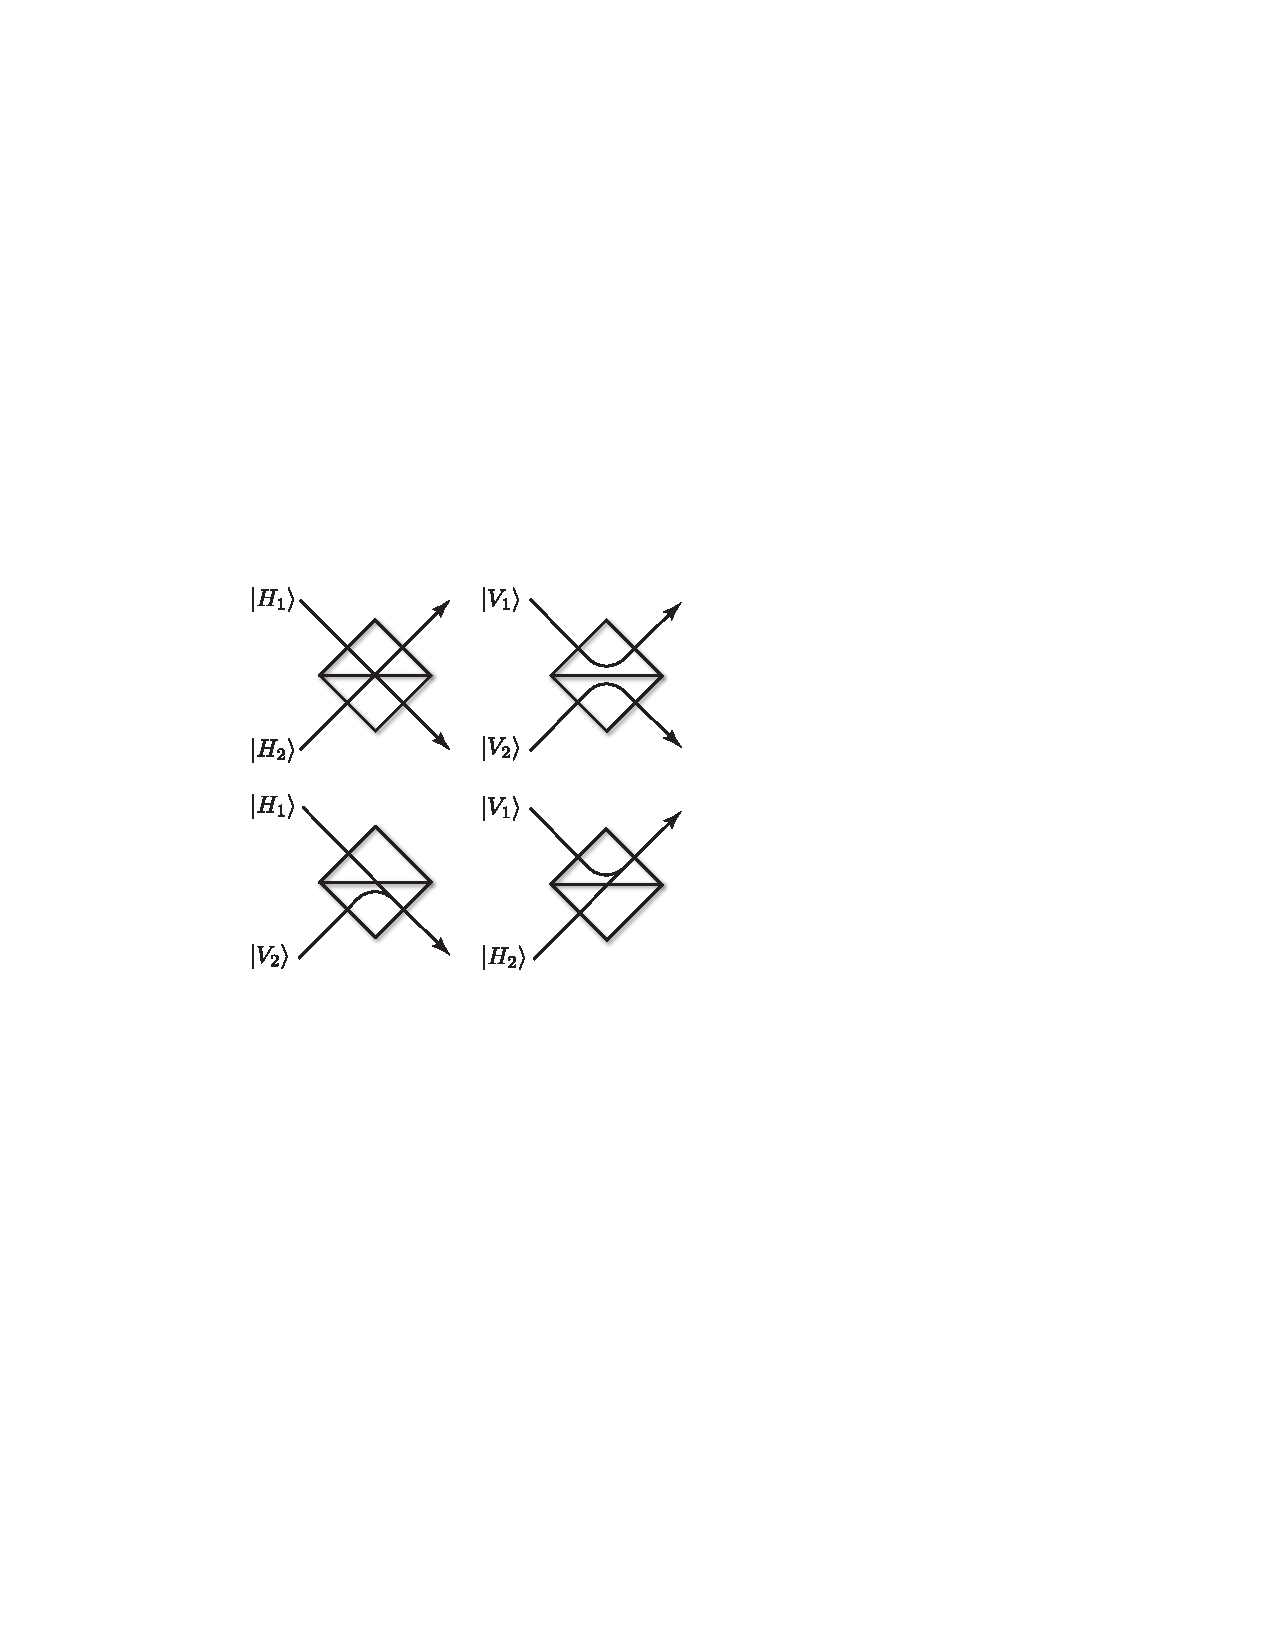
\includegraphics[width=0.75\columnwidth]{partial_bell}
\caption{Partial Bell state projection using a polarising beamsplitter (PBS). The PBS completely transmits horizontally polarised light, whilst completely reflecting vertically polarised light. Shown are the four possible two-photon input states, and the respective trajectories followed by the photons. To complete the partial Bell projection we measure the output modes in the diagonal basis, \mbox{$\ket{\pm} = \frac{1}{\sqrt{2}}(\ket{H}\pm\ket{V})$}, such that horizontally and vertically polarised photons cannot be distinguished. If the input state was $\ket{H,H}$ or $\ket{V,V}$, we would measure one photon in each output mode (both transmitted or both reflected). Since the detectors cannot distinguish $\ket{H}$ from $\ket{V}$, this effectively projects us onto the coherent superposition of both possibilities (`which-path erasure'), implementing the measurement projector \mbox{$\hat\Pi_\mathrm{Bell}^\pm = \ket{H,H}\bra{H,H}\pm\ket{V,V}\bra{V,V}$}. If, on the other hand, we measure two photons at one output mode, we know with certainty what the polarisations of both incident photons were and we probabilistically implement one of the projectors \mbox{$\hat\Pi_
\mathrm{HV}=\ket{H,V}\bra{H,V}$} or \mbox{$\hat\Pi_
\mathrm{VH}=\ket{V,H}\bra{V,H}$}, effectively performing polarisation-resolved detection upon both modes. The practical outcome of this is that, when using a PBS to prepare cluster states, with probability $1/2$ we are able to successfully fuse two smaller cluster states together into a larger one, and with probability $1/2$ we fail to do so, instead removing two qubits from the clusters.} \label{fig:partial_bell}
\end{figure}

While partial Bell state projection using a PBS is relatively straightforward, LOQC CNOT gates (which are very desirable owing to their near-determinism) are very technologically challenging, with drastic resource overheads, particularly for high success probability. Thus, outsourcing them to the cloud may be very economically efficient.

%
% Detector Banks
%

\subsubsection{Detector banks}

In the case of an entire quantum computation, whether it be in the circuit model or cluster state model, many qubits may need to be measured independently, adding a direct multiplicative overhead in the required number of detectors. Furthermore, in protocols requiring fast-feedforward, the detectors may be required to have very fast time-response. These requirements can quickly become very challenging and expensive, further exaggerating the desirability of outsourcing the measurement stage.

%
% Matter Qubits
%

\subsubsection{Matter qubits}

Many non-optical systems can be indirectly measured by first entangling optical states with the matter qubits and then measuring the optical state. Because of the entanglement, projective measurement on the optical state teleports the measurement onto the matter qubit.

In Fig.~\ref{fig:barrett_kok} we illustrate a scheme for entangling two $\lambda$-configuration atoms using which-path erasure. Consider just one of these qubits in isolation. If a $\pi$-pulse is applied to the atom, the $\ket{\!\downarrow}$ state is excited to the $\ket{e}$ state, after which, upon relaxation, emits a photon. Thus, upon measurement, the presence or absence of a photon directly indicates whether the qubit was in the $\ket{\!\uparrow}$ or $\ket{\!\downarrow}$ state.

The attractive feature of this, is that although the matter qubit is stationary, its indirect measurement via optical coupling may be performed over arbitrary distances across the optical network, allowing the measurement stage to be outsourced. This includes entangling measurements, useful for, for example, cluster state preparation (Sec.~\ref{sec:CSQC}).

%
% Evolution
%

\subsection{Evolution}

The evolution of optical states represents an extremely broad category of quantum operations, including passive linear optics, post-selected linear optics, non-linear optics, and light-matter interactions, amongst many others. Clearly even this restricted list presents technological challenges, inaccessible to many users. However, the fundamental error mechanisms are essentially the same as for the measurement errors listed above.

The notable exception is non-linear optics, whereby additional errors in the photon-number degree of freedom or phase-space are possible, since, unlike linear optics, photon-number needn't be conserved in general. This additional degree of freedom in error mechanisms may be accommodated for by introducing an error measure capturing confusion in photon-number or unwanted phase-space transformations. For example, for a given non-linear interaction, error metrics quantifying error bounds on phase-space transformations, such as fluctuation in squeezing or displacement operations, could be employed, which can be represented as metrics, and are therefore compatible with the error metric formalism upon which QTCP is based\footnote{For example, consider unwanted phase-space displacements as an error model. The coherent amplitudes of displacements accumulate additively, and therefore satisfy our notion of an error metric.}.

%
% Random Number Generation
%

\subsection{Random number generation}

Perhaps the simplest quantum information processing task is that of perfect random number generation. True random numbers have widespread applications in cryptography, Monte-Carlo simulations, and any type of randomised algorithm.

Classical random number generators are actually deterministic, but so difficult to predict that we accept them to be as good as random. But for some applications this isn't enough, and we must make sure that no correlations of any type exist between different random numbers, or between the random numbers and their environment.

This can be achieved in many different ways quantum mechanically. Ultimately, they are all based on the Heisenberg uncertainty principle, that certain quantum mechanical measurements yield uncertainty. Most trivially, we can prepare a photon with diagonal polarisation, \mbox{$\ket{+} = \frac{1}{\sqrt{2}}(\ket{H}+\ket{V})$}, and then measure it in the horizontal/vertical polarisation basis (given by measurement projectors \mbox{$\ket{H}\bra{H}$} and \mbox{$\ket{V}\bra{V}$}). Assuming the device is perfectly implementing this procedure, we will measure a perfect random 50/50 distribution between $\ket{H}$ and $\ket{V}$. Equivalently, measuring one half of a polarisation-entangled photon-pair, \mbox{$\frac{1}{\sqrt{2}}(\ket{H}\ket{H}+\ket{V}\ket{V})$}, yields the same outcome.

The cynics amongst us might question the non-determinism of the laws of Nature, and ask whether quantum random numbers really are truly random (in the sense of non-determinism), or whether they also are just too hard to predict that we treat them as effectively random. The answer to this is that it has been proven that quantum mechanics is inconsistent with `hidden variable theories' \cite{Bell}, i.e that there is an underlying, but inaccessible determinism in the world, which is guiding quantum measurements in a completely deterministic manner. This disproof effectively validates the notion of quantum mechanical perfect random number generation.

Consider the scenario where a client needs a stream of true random numbers for use in her Monte-Carlo simulation algorithm or as a secret key for her email encryption. She has limited quantum resources herself, so she outsources it to her better-equipped mate. Depending on her own resource limitations and potential security considerations, her friend could either: (1) implement the full protocol described above, providing her with a classical random bitstream; or (2) only take care of photon generation, providing her with a perpetual source of high-quality photons for her to measure herself using a simple photo-detector. (1) and (2) would both be suitable if the intention was to apply the source of randomness to a Monte-Carlo simulation. But in a cryptographic scenario, where the randomness is being used for key generation, clearly Alice could not outsource the measurement stage without revealing her secret key. In this instance, Bob can act as the provider of photons, while Alice does the measurements herself so as to keep her random bit-string secret.

This scenario is an obvious example of where a UDP-like {\sc Send And Forget} protocol may be viable. Unlike most other applications, Bob is broadcasting a stream of identical, pure quantum states, that are not entangled with any peripheral system, and are easily replicated, with no correlations between distinct photons. Thus, if any particular photon fails to reach Alice, it matters not, as she can simply await the next one emanating from Bob's bombardment of photons.

%
% Memory
%

\subsection{Memory} \label{sec:memory}

A final building block, that will be essential in many networks, is quantum memory, which simply delays a packet by some fixed amount of time, ideally implementing an identity channel. This will be required when, for example, quantum data packets reach a network bottleneck, and face one of two options: wait, or be discarded. As discussed earlier, discarding quantum packets is often a highly undesirable enterprise, as they often cannot be easily recreated, most notably when entangled with other systems.

Quantum memory is modelled in our network graph representation as per Fig.~\ref{fig:memory}, via a self-loop implementing a process that delays packets. Ideally, the associated process should implement the identity operation in all degrees of freedom, except the temporal one, affecting only the {\sc Lifetime} metric of the packets passing through it, incrementing it by the duration of the quantum memory.

Note that this is not directly compatible with conventional shortest-path algorithms, which ignore self-loops. One approach is to modify our strategy optimisation algorithms to accommodate self-loops. Alternately, we could construct a `virtual' graph, obtained by adding additional nodes to the network, with connections determined by `unravelling' the self-loops. For example, in Fig.~\ref{fig:memory}, we could eliminate the self-loop, and instead replace $B$ with multiple redundant nodes in parallel between $A$ and $C$, each associated with their own latency cost.

\begin{figure}[!htb]
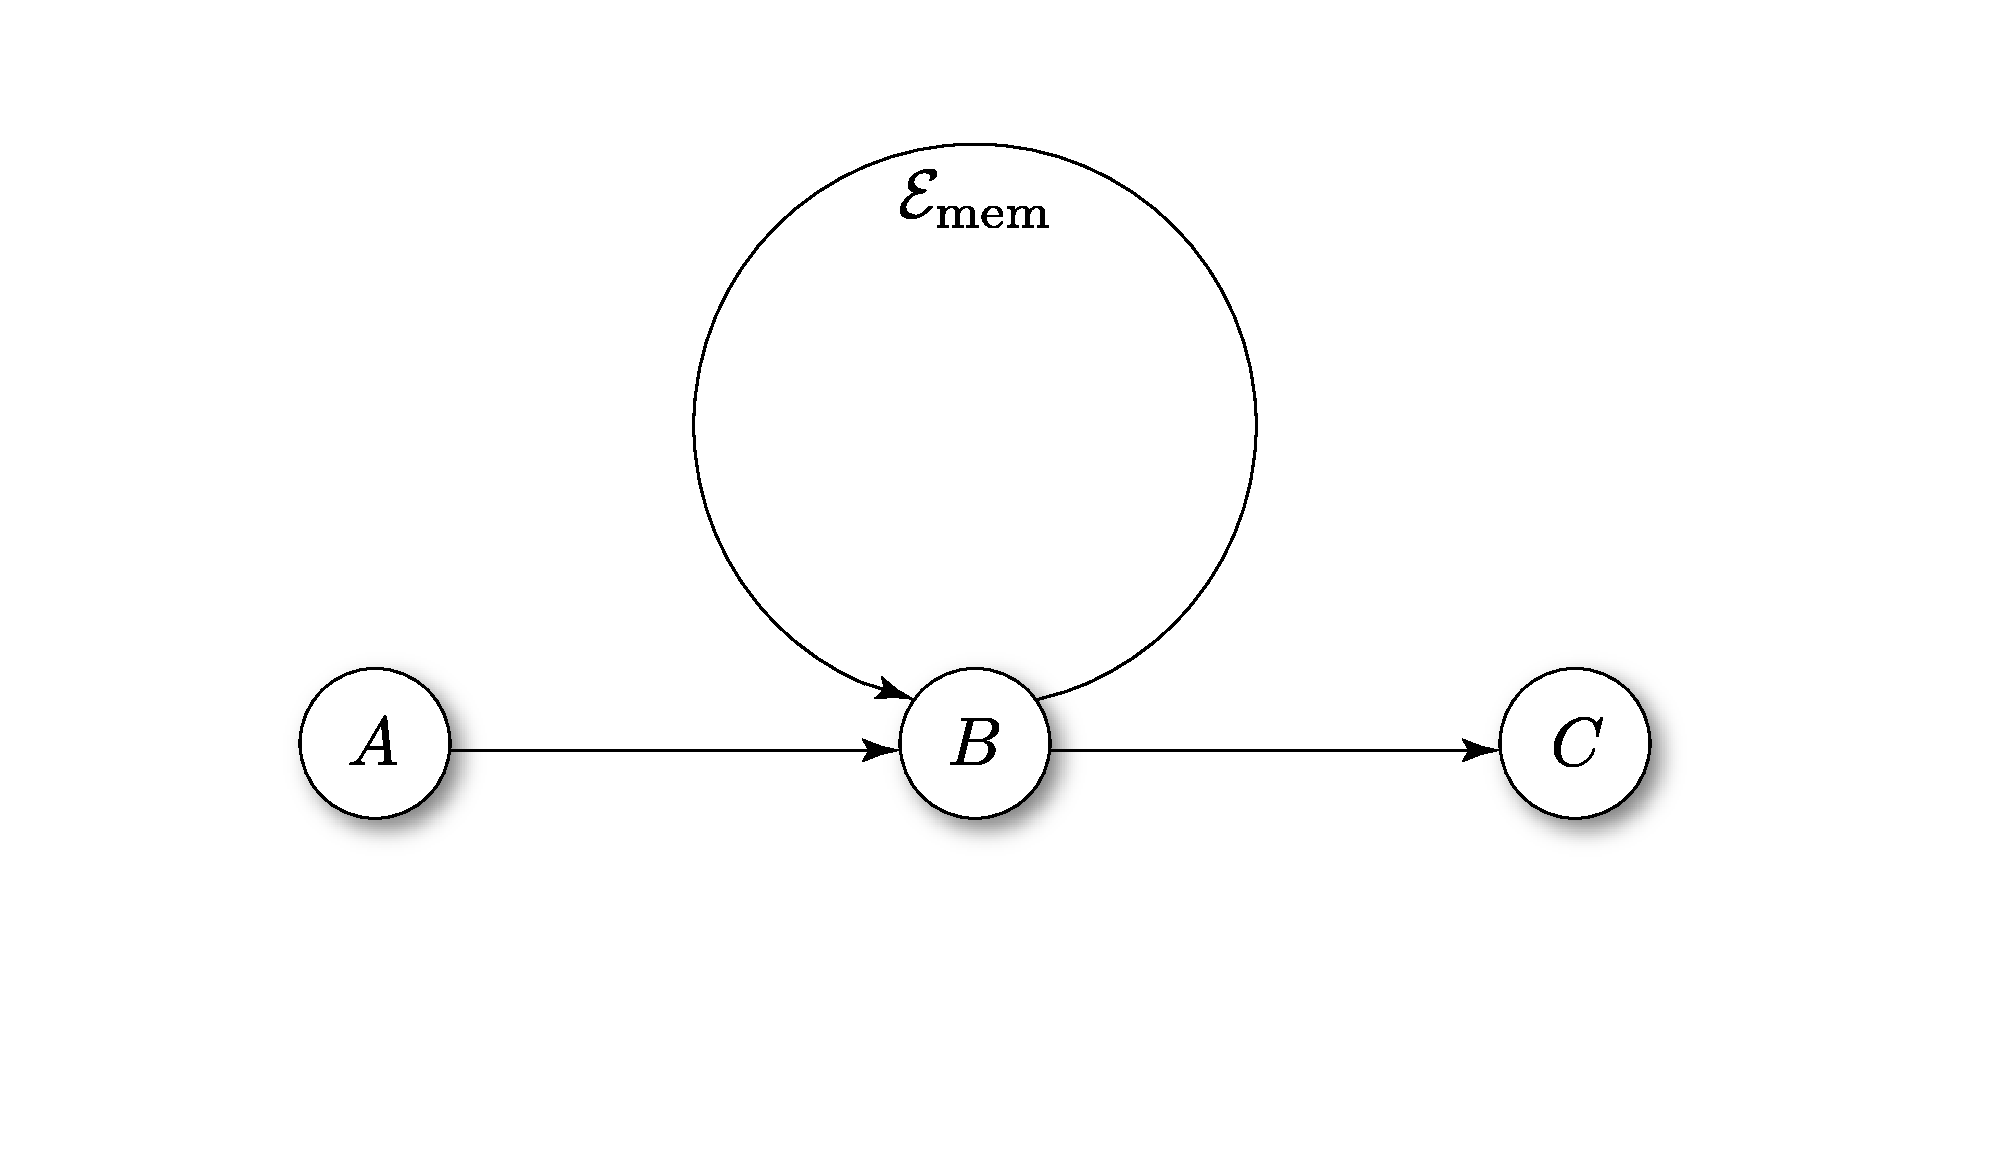
\includegraphics[width=0.7\columnwidth]{memory}
\caption{Simple model for a quantum memory via a self-loop that passes through a memory process, $\mathcal{E}_\mathrm{mem}$. Ideally, $\mathcal{E}_\mathrm{mem}$ does not affect any of the costs or attributes of states passing through the link, except for the latency cost, which is incremented according to the duration of the memory.} \label{fig:memory}
\end{figure}

At the physical level, there are two main approaches we could use to put optical states into memory. The first is simply to employ delay lines, either in free-space or in fibre. The second is to interface the state with a non-optical system with a long lifetime, which holds the information content until needed and out-coupled. This can be achieved using, for example, the light-matter interfacing techniques discussed in Sec.~\ref{sec:opt_inter}.

The former is experimentally straightforward, but plagued by loss, and is only suitable over short timescales, on the order of nanoseconds. The latter is more experimentally challenging, but can achieve longer storage times, limited by the lifetime ($T_1$- and $T_2$-times) of the non-optical system. For some physical systems, this can be very high, on the order of milliseconds for atomic ensemble qubits \cite{bib:Duan01, bib:Duan02, bib:LauratKimble07}, for example, which is typically adequate for the purposes of waiting out network bottlenecks.

%
% Optical Interfacing
%

\subsection{Optical interfacing} \label{sec:opt_inter}

Unless the entire pipeline of quantum operations through the course of a protocol is all-optical, there will be a need to exchange information between physical systems, for example via light-matter interactions \cite{bib:Cohen-Tannoudji92}. The archetypal interface is that between a photonic qubit in the \mbox{$\{\ket{0},\ket{1}\}$} photon-number basis, and a two-level matter qubit in the $\ket{g}$ (ground) and $\ket{e}$ (excited) state basis. Examples include atoms in cavities, atomic ensembles \cite{bib:Chou05}, nitrogen-vacancy (NV) centres, and quantum dots.

In the case of a photon interacting with a two-level matter qubit, the interface can be expressed as an interaction Hamiltonian of the form,
\begin{align} \label{eq:two_level_hamil}
\hat{H}_\mathrm{int} = \hbar \chi (\hat{a}\,\hat\sigma^+ + \hat{a}^\dag\hat\sigma^-),
\end{align}
where $\hat{a}$ ($\hat{a}^\dag$) is the photonic annihilation (creation) operator, $\hat\sigma^\pm$ are the Pauli spin-flip operators, and $\chi$ is the interaction strength. The interpretation of this Hamiltonian is very clear upon inspection -- the annihilation (creation) of a photon is associated with the excitation (relaxation) of the two-level matter system, thereby directly exchanging quantum information between the two systems, as shown in Fig.~\ref{fig:opt_int}.

\begin{figure}[!htb]
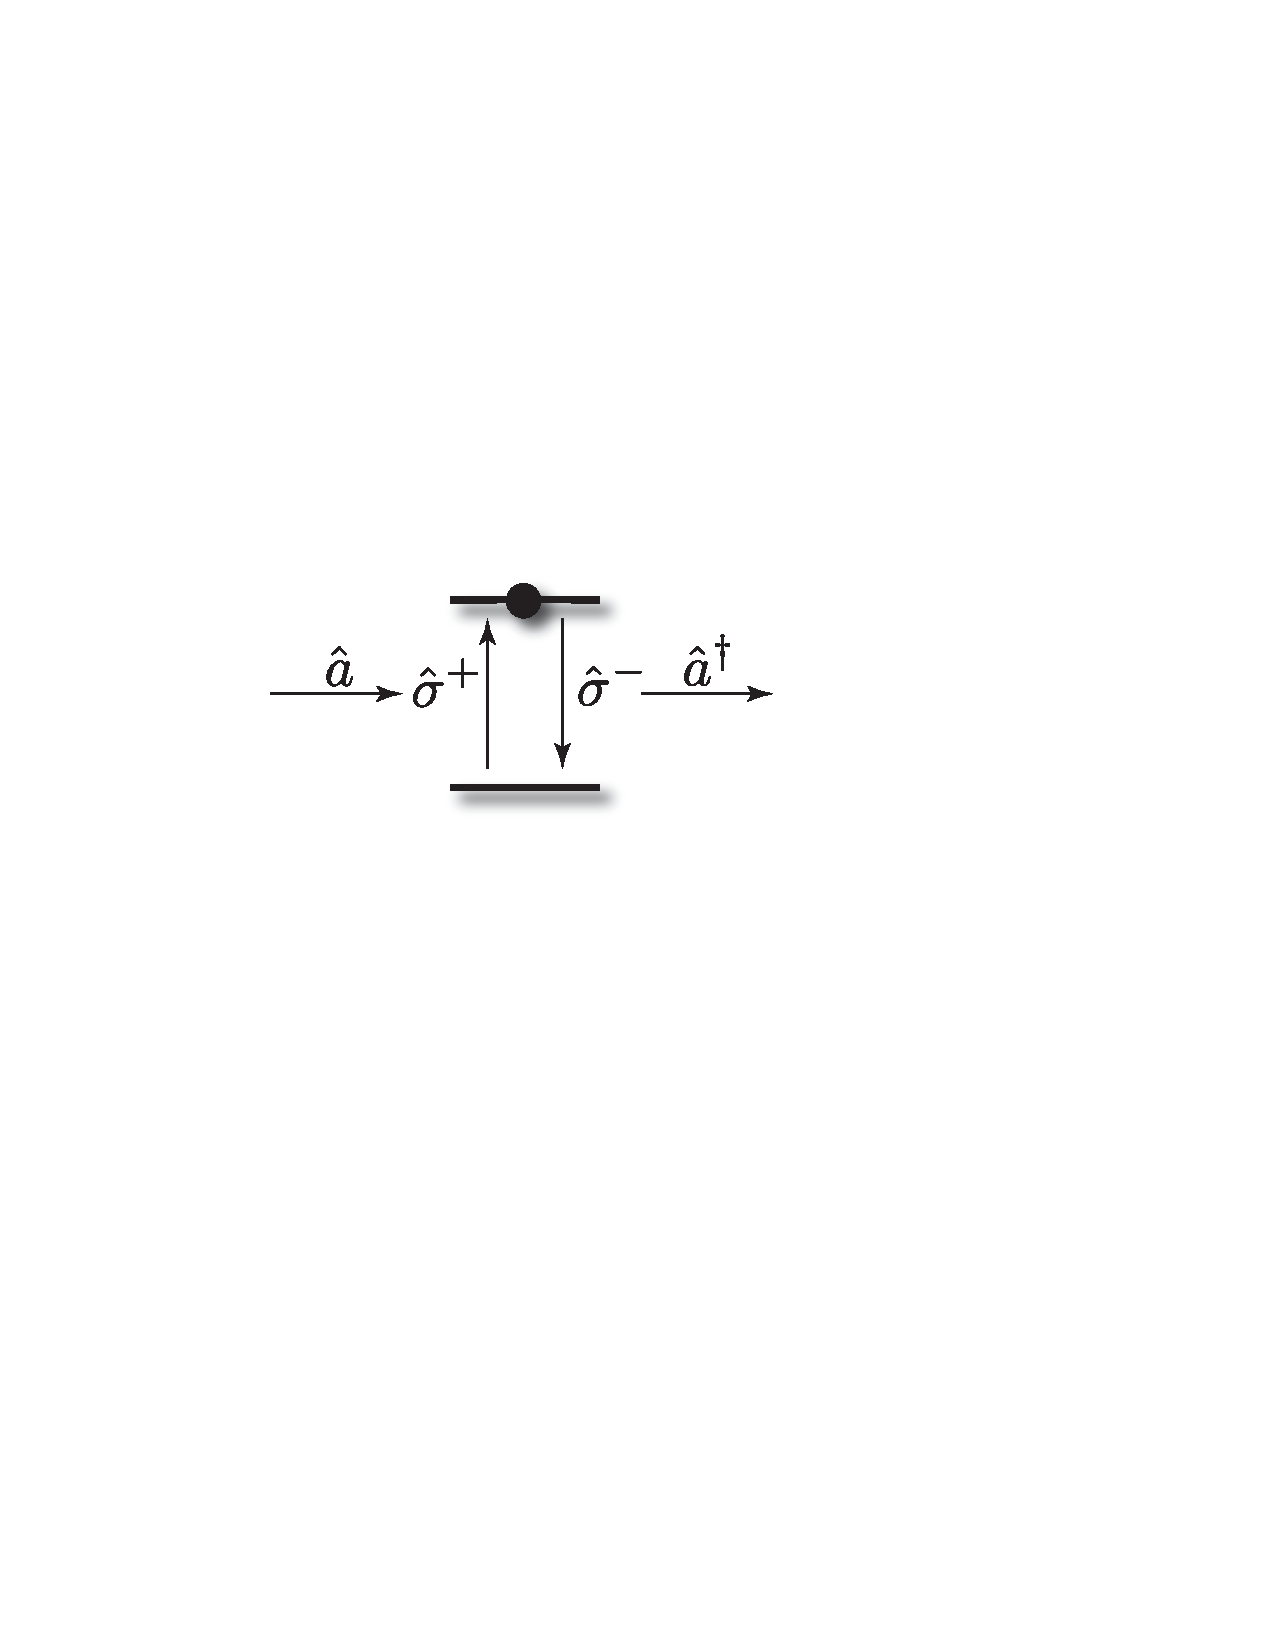
\includegraphics[width=0.6\columnwidth]{opt_inter}
\caption{Light-matter interfacing between a single-photon state ($\hat{a}$, $\hat{a}^\dag$) and a two-level matter qubit ($\ket{g}$, $\ket{e}$). The absorption (emission) of a photon is associated with the excitation (relaxation) of the matter qubit ($\hat\sigma^\pm$).} \label{fig:opt_int}
\end{figure}

Alternately, one can easily optically interface with a $\lambda$-configuration system, as described in Fig.~\ref{fig:barrett_kok}. 

%
% Entanglement Purification
%

\subsection{Entanglement purification} \label{sec:ent_purif}

Entangled states, most notably Bell-pairs (Sec.~\ref{sec:bell_state_res}), play a central role in many quantum technologies. These maximally entangled states are easily represented optically using polarisation encoding of single photons, and can be non-deterministically prepared directly using SPDC (Sec.~\ref{sec:single_phot_src}), or post-selected linear optics \cite{???}.

Bell-pairs are the basis for building cluster states (Sec.~\ref{sec:CSQC}), some quantum cryptography protocols (Sec.~\ref{sec:QKD}), and quantum teleportation (Sec.~\ref{sec:teleport}), to name just a few applications. Therefore distributing entangled states with the highest entanglement metrics is extremely important. In short, entanglement can be considered a valuable quantum resource (discussed in detail in Sec.~\ref{sec:ent_ultimate}), upon which many other protocols may be built.

Suppose Alice and Bob share an entangled pair. Quantum mechanics, specifically the very definition of entanglement itself, prohibits local operations performed by Alice and Bob from increasing the level of entanglement. However, if Alice and Bob share multiple pairs, they can perform an operation known as \emph{entanglement purification} or \emph{entanglement distillation}, whereby two lower-fidelity entangled pairs are consumed and projected onto a single entangled pair with higher fidelity \cite{bib:PRA_53_2046, bib:PRA_54_3824, bib:PRL_77_2818}. Such protocols will be extremely useful in protocols where achieving the highest possible degree of entanglement is paramount, for example when error thresholds must be achieved for the purpose of error-correction and fault-tolerance \cite{bib:NielsenChuang00}.

Taking two polarisation-encoded photonic Bell-pairs, say $\ket{\Psi^+}$ and subjecting them to a dephasing error model yields a mixed state of the form,
\begin{align}
\hat\rho_\mathrm{in} = F\ket{\Psi^+}\bra{\Psi^+} + (1-F)\ket{\Psi^-}\bra{\Psi^-},
\end{align}
where $F$ is the entanglement fidelity, which is a function of the dephasing rate. Note that $\ket{\Psi^+}$ and $\ket{\Psi^-}$ are related by local phase-flip operations ($\hat{Z}$) applied to either qubit,
\begin{align} \label{eq:psi_minus}
\ket{\Psi^-} = \hat{Z}_A \ket{\Psi^+} = \hat{Z}_B \ket{\Psi^+}.
\end{align}

A linear optics entanglement purification protocol can be simply implemented using two polarising beamsplitters PBS's \cite{bib:Pan01, bib:Pan03}. Alice uses one PBS to interfere the photons from her side of each of the photon pairs, measuring one output only, which implements a non-deterministic, partial Bell projection. Bob does the same on his side. What's left is one photon in Alice's hands and one in Bob's. When successful, they will now be sharing a single entangled pair of higher Bell state fidelity than the two starting states. The protocol is shown in Fig.~\ref{fig:ent_purif_prot}.

Note that when using PBS's to perform the Bell projections, the protocol is necessarily non-deterministic, since PBS's are only able to distinguish two of the four Bell states. Thus, each PBS has a success probability of $1/2$. And there are two PBS's per instance of the protocol, therefore the net success probability is $1/4$. When concatenated, $n$ applications of the protocol thus has an exponentially low success probability of $1/4^n$. This could be overcome using deterministic CNOT gates, but these are challenging using linear optics.

Furthermore, the protocol consumes two Bell-pairs upon each trial, only one quarter of which are successful. Thus, on average, 8 Bell-pairs are consumed for every purified Bell-pair prepared, and the expected number of Bell-pairs required to perform $n$ iterations of entanglement purification grows exponentially as $8^n$.

\begin{figure}[!htb]
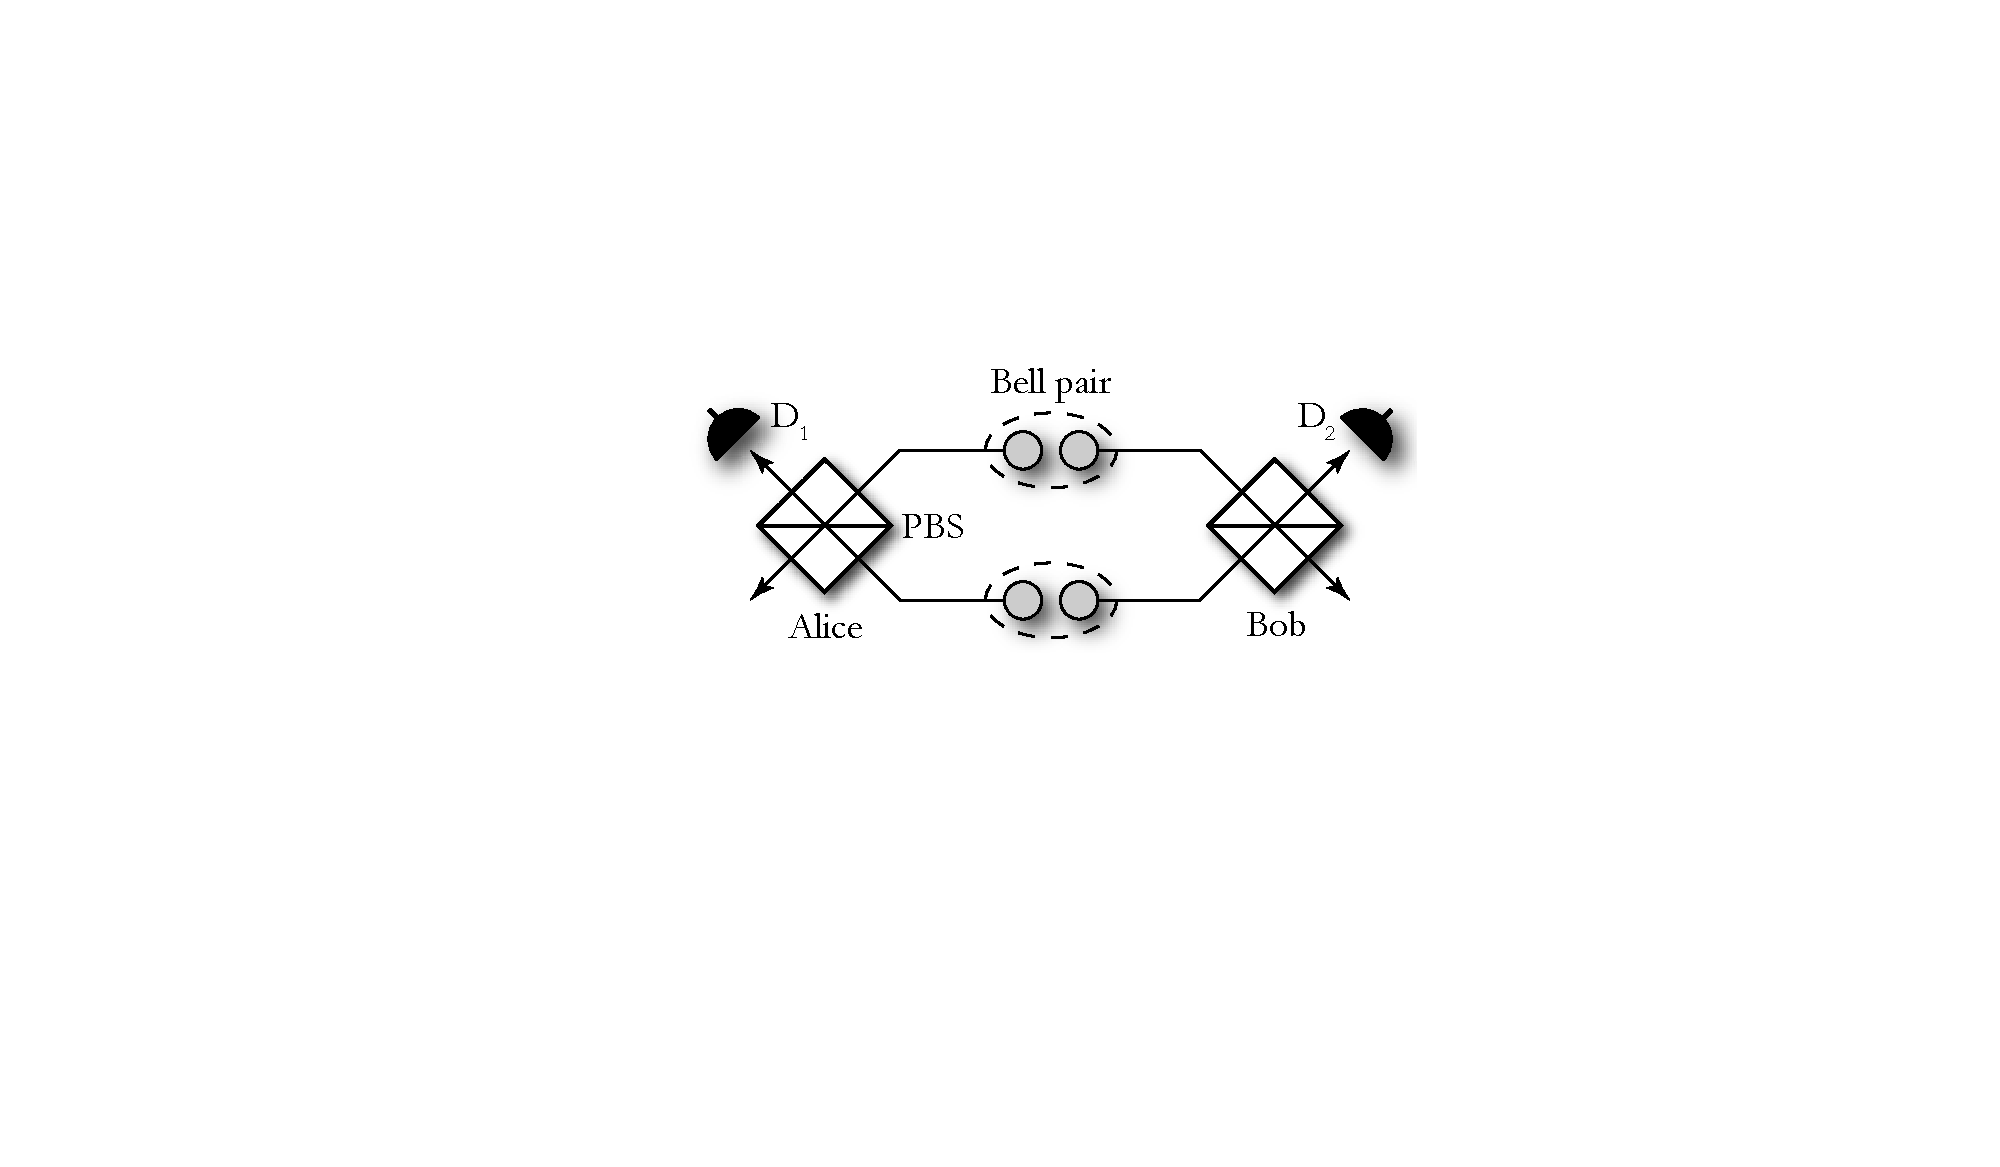
\includegraphics[width=0.9\columnwidth]{ent_purif_prot}
\caption{Elementary entanglement purification using linear optics. Two Bell-pairs are distributed between Alice and Bob, each of which has been subject to a dephasing error model. Alice and Bob perform Bell measurements on their two qubits using PBS and polarisation-resolved photo-detection ($D_1$ and $D_2$). Upon successful Bell state projection (Bell measurements are necessarily non-deterministic using linear optics), Alice and Bob will share a single Bell-pair with higher fidelity than the two input pairs.} \label{fig:ent_purif_prot}
\end{figure}

Specifically, the relationship between the input ($F_\mathrm{in}$) and output ($F_\mathrm{out}$) fidelities of the protocol is,
\begin{align}
F_\mathrm{out} = \frac{{F_\mathrm{in}}^2}{{F_\mathrm{in}}^2 + (1-F_\mathrm{in})^2}.
\end{align}
This input/output relationship is shown in Fig.~\ref{fig:ent_purif}.

\begin{figure}[!htb]
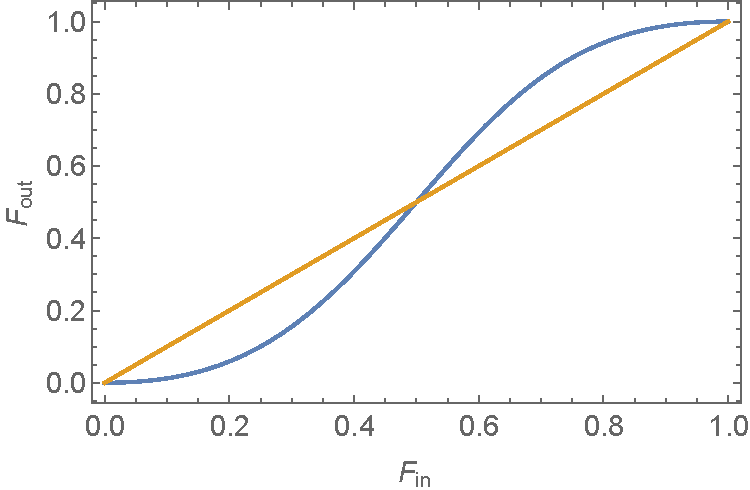
\includegraphics[width=\columnwidth]{ent_purif}
\caption{Entanglement purification of two polarisation-encoded, photonic Bell-pairs. $F_\mathrm{in}$ ($F_\mathrm{out}$) are the input (output) fidelities of the Bell-pairs. The protocol consumes two Bell-pairs for every one purified pair. The straight line represents the break-even point in terms of state fidelity, above which the protocol enhances fidelity, and below which reduces it. This places a strict bound on the fidelity of Bell-pairs reaching the purifier. This equates to route cost, if measured by the fidelity metric, stipulating network performance requirements. This threshold requirement presents an example of where an {\sc All or Nothing} strategy might be appropriate.} \label{fig:ent_purif}
\end{figure}

Note that there is a break-even point, above which the protocol strictly increases fidelity, and below which strictly decreases it. This occurs at \mbox{$F_\mathrm{in}=1/2$}. Provided pairs can be communicated above this fidelity threshold, bootstrapped application of the protocol could be employed to boost entanglement fidelity asymptotically close to unity (but with exponential resource overhead, since each operation consumes two pairs to produce one). But below this threshold it is impossible to recover any more entanglement than we started with. This provides an example of an application where the protocol being implemented dictates strict requirements on network cost metrics. Specifically, assuming perfect Bell-pairs to begin with, the routes by which they are communicated must ensure entanglement fidelities of at least \mbox{$F=1/2$} upon reaching destination. Here a type of {\sc All or Nothing} networking strategy would be applicable -- if the fidelity requirement is not met, the state cannot be purified and might as well be thrown away to make way for other traffic.

A theoretical analysis of this protocol has been performed, accounting for mode-mismatch in the protocol \cite{bib:RohdeOptEntPur06}, where it was found than mode-mismatch shifts the break-even point upwards, and lowers the maximum value of $F_\mathrm{out}$ -- with more mode-mismatch, a higher starting fidelity is required to break even, and we achieve a lower, sub-unity output fidelity. In this case, a cost function that combines the dephasing and mode-mismatch metrics of the network will be required.

Importantly, this protocol is based on partial Bell state measurement, and therefore does not require interferometric stability, only high HOM visibility, thus making stabilisation comparatively easy over long distances.

Entanglement purification can also be performed using physical encodings other than single photons. For example, this has been demonstrated in Gaussian CV quantum states \cite{bib:Duan00}.

%
% Quantum State Teleportation
%

\subsection{Quantum state teleportation} \label{sec:teleport}

Quantum state teleportation \cite{???, bib:PRL_70_1895} is an essential ingredient in many higher-level protocols. It forms the basis of cluster state quantum computing (Sec.~\ref{sec:CSQC}), some QEC codes, the KLM linear optics quantum computing scheme (Sec.~\ref{sec:KLM_univ}), and can act as a mediator for long-range transmission of quantum states, amongst others.

In the standard teleportation protocol, Alice begins with a single qubit,
\begin{align}
\ket\phi = \alpha\ket{0} +\beta\ket{1},
\end{align}
which she would like to teleport to Bob. Importantly, no quantum communication between the two is allowed, since obviously this would make the problem trivial. However, classical communication is allowed (and turns out to be necessary), and furthermore they share an entangled Bell-pair. Thus, Alice begins with two qubits, and Bob begins with one -- his half of the entangled pair onto which Alice's state ought to be teleported. The initial state is therefore,
\begin{align}
\ket\psi_\mathrm{in} &= \ket{\phi}_{A_1} \ket{\Psi^+}_{A_2,B} \\
&= \frac{1}{\sqrt{2}} (\alpha\ket{0}_{A_1}+\beta\ket{1}_{A_1}) (\ket{0}_{A_2}\ket{1}_B + \ket{1}_{A_2}\ket{0}_B). \nonumber
\end{align}

The first step of the protocol is for Alice to perform a two-qubit entangling measurement on her two qubits, projecting onto the Bell basis (Eq.~\ref{eq:bell_basis}). She obtains one of four measurement outcomes. For illustration, suppose she measures the $\ket{\Psi^+}$ outcome. Then the projected state is,
\begin{align}
\ket\psi_\mathrm{proj}^{\Psi^+} &= \bra{\Psi^+}_{A_1,A_2} \ket\psi_\mathrm{in} \nonumber \\
&= \frac{1}{\sqrt{2}} \bra{\Psi^+}_{A_1,A_2}\ket\psi_{A_1}(\ket{0}_{A_2}\ket{1}_B + \ket{1}_{A_2}\ket{0}_B) \nonumber \\
&= \frac{1}{2} (\bra{0}_{A_1}\bra{1}_{A_2} + \bra{1}_{A_1}\bra{0}_{A_2}) \nonumber \\
&\cdot (\alpha\ket{0}_{A_1}+\beta\ket{1}_{A_1})(\ket{0}_{A_2}\ket{1}_B + \ket{1}_{A_2}\ket{0}_B) \nonumber \\
&= \frac{1}{2} (\alpha \ket{0}_B + \beta \ket{1}_B)\nonumber \\
&= \frac{1}{2} \ket\phi_B,
\end{align}
which is Alice's initial state. For all four possible Bell measurement outcomes we have,
\begin{align}
\ket\psi_\mathrm{proj}^{\Psi^+} &= \frac{1}{2} (\alpha \ket{0}_B + \beta \ket{1}_B) \nonumber \\
&= \frac{1}{2} \ket\phi_B, \nonumber \\
\ket\psi_\mathrm{proj}^{\Psi^-} &= \frac{1}{2} (\alpha \ket{0}_B - \beta \ket{1}_B) \nonumber \\
&= \frac{1}{2} \hat{Z}\ket\phi_B, \nonumber \\
\ket\psi_\mathrm{proj}^{\Phi^+} &= \frac{1}{2} (\alpha \ket{1}_B + \beta \ket{0}_B) \nonumber \\
&= \frac{1}{2} \hat{X} \ket\phi_B, \nonumber \\
\ket\psi_\mathrm{proj}^{\Phi^-} &= \frac{1}{2} (\alpha \ket{1}_B - \beta \ket{0}_B) \nonumber \\
&= \frac{1}{2} \hat{X}\hat{Z}\ket\phi_B,
\end{align}
which are all locally equivalent to $\ket\phi$ under Pauli gates, and can be corrected by Bob, given communication of the classical Bell measurement outcome provided by Alice. The full protocol is described in Alg.~\ref{alg:state_teleport}.

\begin{table}[!htb]
\fbox{\parbox{0.965\columnwidth}{\tt
function StateTeleportation($\ket\phi_{A_1}$, $\ket{\Phi^+}_{A_2,B}$):
\begin{enumerate}
    \item Alice prepares the state $\ket\phi_{A_1}$, which she would like to teleport to Bob.
    \item Alice and Bob share the Bell-pair $\ket{\Phi^+}_{A_2,B}$.
    \item Alice performs a Bell state projection between qubits $A_1$ and $A_2$.
    \item Alice communicates the classical measurement outcome to Bob - one of four outcomes.
    \item Bob applies an appropriate local correction to his qubit - some combination of the Pauli operators $\hat{X}$ and $\hat{Z}$ - according to the classical measurement outcome.
    \item Bob is left with the state $\ket\phi_B$.
    \item $\Box$
\end{enumerate}
\begin{align}
\Qcircuit @C=1em @R=1.6em {
    \lstick{\ket\phi} & \qw & \multimeasureD{1}{\text{Bell}} & \cw  & \control \cw \\
    \lstick{} & \qw & \ghost{\text{Bell}} & \control \cw & \cwx \\
    \lstick{} & \qw & \qw & \gate{X} \cwx & \gate{Z} \cwx & \qw & \qw & \ket\phi
    \inputgroupv{2}{3}{.8em}{.8em}{\ket{\Phi^+}}
} \nonumber
\end{align}
}}
\caption{Quantum state teleportation of a single qubit.} \label{alg:state_teleport}
\end{table}

In general, the protocol is deterministic, although using PBS's to perform partial Bell measurements, the success probability is $1/2$.

The question now is what error metrics apply and how do they accumulate in the teleportation protocol. The answer is straightforward -- the final teleported qubit accumulates all local Pauli errors (e.g dephasing or depolarisation) associated with Alice's input state as well as any that acted upon the shared Bell-pair. That is, the errors get teleported along with the state being teleported, plus any errors on the Bell-pair.

In the case of loss, loss of either of Alice's qubits will immediately be detected when she performs her Bell measurement. Thus, loss becomes a located error, and the knowledge of the error allows the associated packet to be discarded and the sender and recipient notified. On the other hand, loss on Bob's qubit will behave no differently than loss acting on an ordinary qubit channel.

Thus, in terms of Pauli errors, no special treatment is required by the QTCP protocol -- it is almost as if the teleportation protocol weren't there. And in terms of loss, the Bell state projection diagnoses lost qubits, allowing appropriate action to be taken, which is actually better than if the error were undiagnosed.

The total resources required to teleport a single-qubit state are:
\begin{enumerate}
\item The qubit to be teleported.
\item A shared Bell-pair.
\item A two-qubit measurement in the Bell basis.
\item The transmission of two classical bits.
\item Two classically controlled Pauli gates.
\end{enumerate}

This is more costly than sending the qubit directly over a quantum channel, but may be the only approach if a direct link is not available. In the context of an internet where entanglement distribution is treated as the fundamental resource (Sec.~\ref{sec:ent_ultimate}), state teleportation is the natural approach for communicating quantum states, since no quantum communication of any kind is required once the two parties have a shared Bell-pair between them.

The important feature of this protocol to note is that there is no direct quantum communication between Alice and Bob, only a classical communications channel. Rather, the Bell-pair mediates the transfer of quantum information, despite there being no direct quantum channel between Alice and Bob.

Relying on teleportation rather than direct quantum communication makes frugal use of quantum channels, since there is no need for direct quantum routes between every pair of nodes in the network. Instead, each node need only have a direct one-way quantum link with the central authority responsible for entanglement distribution, thereby significantly reducing the complexity of the topology of the quantum network.

The Bell state measurement can be implemented either using a CNOT gate, or as a non-deterministic partial Bell state measurement using a PBS (Sec.~\ref{sec:bell_proj}).

%
% Quantum Gate Teleportation
%

\subsection{Quantum gate teleportation} \label{sec:teleport_gate}

Using quantum \emph{state} teleportation as a primitive building block, quantum \emph{gate} teleportation may be implemented \cite{bib:GottesmanChuang99}. Here rather than teleporting a quantum state from one physical system to another, we teleport the action of a quantum gate onto a physical system (archetypically a maximally entangling two-qubit gate, such as a CNOT gate).

The general outline of the derivation of the protocol for teleporting a CNOT gate onto a two-qubit state is shown in Alg.~\ref{tab:gate_teleport}.

\begin{table}[!htb]
\fbox{\parbox{0.965\columnwidth}{\tt
function GateTeleportation($\ket\psi_A\ket\phi_B$):\
\begin{enumerate}
\item We wish to apply a CNOT gate to \mbox{$\ket\psi_{A}\ket\phi_{B}$}.
\item Introduce two additional qubits, $C$ and $D$.
\item Teleport states \mbox{$\ket\psi_{A}\to\ket\psi_C$}, \mbox{$\ket\psi_{B}\to\ket\psi_D$}.
\item Apply \mbox{$\hat{\mathrm{CNOT}} \ket \psi_C \ket\phi_D$}.
\begin{align}
\Qcircuit @C=1em @R=1.6em {
\lstick{\ket\psi} & \qw & \multimeasureD{1}{\text{Bell}} & \cw  & \control \cw \\
\lstick{} & \qw & \ghost{\text{Bell}} & \control \cw & \cwx \\
\lstick{} & \qw & \qw & \gate{X} \cwx & \gate{Z} \cwx & \ctrl{1} & \qw & \qw & \qw \inputgroupv{2}{3}{.8em}{.8em}{\ket{\Phi^+}} \\
\lstick{} & \qw & \qw & \gate{X} & \gate{Z} & \targ & \qw & \qw & \qw \inputgroupv{4}{5}{.8em}{.8em}{\ket{\Phi^+}} \\
\lstick{} & \qw & \multimeasureD{1}{\text{Bell}} & \control \cw \cwx & \cwx \\
\lstick{\ket\phi} & \qw & \ghost{\text{Bell}} & \cw  & \control \cw \cwx
} \nonumber
\end{align}
\item The CNOT is a Clifford gate and can therefore be commuted to the front of the Pauli operators to yield a CNOT followed by some different configuration of Pauli operators.
\item The CNOT now acts jointly upon the Bell-pairs that were acting as a resource for the state teleportation, independent of \mbox{$\ket\psi_{A}\ket\phi_{B}$}.
\item Group the CNOT gate and Bell-pairs together, and treat them as a 4-qubit resource state preparation stage, which does not depend on \mbox{$\ket\psi_{A}\ket\phi_{B}$}. 
\item Prepare the 4-qubit resource state, \mbox{$\ket\chi=\hat{\mathrm{CNOT}}_{2,3}\ket{\Psi^+}_{1,2}\ket{\Psi^+}_{3,4}$}, offline in advance.
\item If the CNOT is non-deterministic, employ {\sc Repeat Until Success} to prepare $\ket\chi$.
\item The output state is \mbox{$\hat{\mathrm{CNOT}}_{C,D} \ket\psi_{C}\ket\phi_{D}$}.
\item $\Box$
\end{enumerate}
\begin{align}
\Qcircuit @C=1em @R=1.6em {
\lstick{\ket\psi} & \qw & \multimeasureD{1}{\text{Bell}} & \cw & \cw & \control \cw \\
\lstick{} & \qw & \ghost{\text{Bell}} & \cw & \cw & \cw \cwx & \control \cw \\
\lstick{} & \qw & \qw & \gate{X} & \gate{Z} & \qw \cwx & \gate{Z} \cwx & \qw & \qw & \qw \\
\lstick{} & \qw & \qw & \gate{X} \cwx & \qw \cwx & \gate{X} \cwx & \gate{Z} \cwx & \qw & \qw & \qw \\
\lstick{} & \qw & \multimeasureD{1}{\text{Bell}} & \control \cw \cwx & \cwx \inputgroupv{2}{5}{0.8em}{4.1em}{\ket{\chi}} \\
\lstick{\ket\phi} & \qw & \ghost{\text{Bell}} & \cw  & \control \cw \cwx
} \nonumber
\end{align}
}}
\caption{Teleporting a CNOT gate onto a two-qubit state.} \label{tab:gate_teleport}
\end{table}

Most notably, gate teleportation is useful when attempting to apply two-qubit entangling operations using non-deterministic gates, in which case gate teleportation allows the non-deterministic elements to be performed offline as a resource state preparation stage, overcoming the non-determinism during the gate application stage. Specifically, when a CNOT gate acting directly upon two qubits fails, it corrupts those qubits, whereas if it fails during a state preparation stage, it can simply be reattempted until a success occurs, without corrupting the target qubits. A concatenated version of the gate teleportation protocol forms the basis for constructing near-deterministic entangling gates in linear optics, to be explained in detail in Sec.~\ref{sec:KLM_univ}.

Quantum gate teleportation effectively reduces the problem of implementing CNOT gates to:
\begin{itemize}
\item Offline preparation of highly-entangled 4-qubit resource states. This needn't be deterministic, since the resource state does not depend on the state to which the CNOT gate ought to be applied.
\item Two Bell measurements.
\item Some configuration of local Pauli operators, dependent upon the Bell measurement outcomes.
\end{itemize}
Importantly, like quantum state teleportation, there is no need for a quantum communications channel between the two parties holding the qubits to which the gate is applied -- classical communication is sufficient.

The gate teleportation idea is conceptually interesting as it converts the problem of `gate application' to that of `state preparation'\footnote{The resource state is prepared from two Bell-pairs and a single CNOT gate. In the absence of a direct source of Bell-pairs, they can be prepared using separable single-qubit states and a CNOT gate. Thus, the full resource state may be prepared from separable single qubits via three CNOT gates.}, by commuting all the entangling operations to the beginning of the protocol. Cluster state quantum computing (Sec.~\ref{sec:CSQC}) is actually the extremity of this logic, whereby an entire quantum computation is transformed into a sequence of state and gate teleportations. One may interpret this to mean that teleportation is a universal resource for quantum computation \cite{bib:GottesmanChuang99}.

The resource states required for gate teleportation are highly-entangled 4-qubit states, which are challenging to prepare, especially in the optical context. Thus, as with cluster states, if the preparation of these resource states were to be outsourced to a specialised provider, they could be in high demand.

%
% Entanglement Swapping
%

\subsection{Entanglement swapping} \label{sec:swapping}

The obvious approach to sending a qubit from Alice to Bob is to send a qubit from Alice to Bob (duh!). However, over long distances this may accrue impractical error rates, particularly losses. The other alternative is to employ the quantum teleportation protocol to teleport the state between the two parties. However, this requires that Alice and Bob first share an entangled Bell-pair, which must itself be distributed across the same distances. Entanglement swapping \cite{???, bib:PRL_71_4287} is the process of taking two Bell-pairs, one held by each party, and swapping the entanglement between them such that the two parties share an entangled state. This procedure can be bootstrapped to progressively swap the entanglement over longer and longer distances, yielding \emph{quantum repeater networks} (Sec.~\ref{sec:rep_net}). The procedure for this protocol is shown in Alg.~\ref{tab:ent_swap} and Fig.~\ref{fig:ent_swap}

\begin{table}[!htb]
\fbox{\parbox{0.965\columnwidth}{\tt
function EntanglementSwapping($\ket{\Phi^+}_{A_1,A_2}, \ket{\Phi^+}_{B_1,B_2}$):
\begin{enumerate}
    \item Alice locally prepares the Bell-pair,
    \begin{align}
    \ket{\Phi^+}_{A_1,A_2}.
    \end{align}
    \item Bob locally prepares the Bell-pair,
    \begin{align}
    \ket{\Phi^+}_{B_1,B_2}.
    \end{align}
    \item The net initial state is,
    \begin{align}
    \ket\psi_\mathrm{in} = \ket{\Phi^+}_{A_1,A_2} \ket{\Phi^+}_{B_1,B_2}.
    \end{align}
    \item Alice sends qubit $A_1$ to third party Eve.
    \item Bob Sends qubit $B_1$ to third party Eve.
    \item Eve performs a Bell projection between $A_1$ and $B_1$, yielding,
    \begin{align}
    \bra{\Phi^+}_{A_1,B_1} \ket\psi_\mathrm{in} = \ket{\Phi^+}_{A_2,B_2}.
    \end{align}
    \item In the case of the other Bell projection outcomes ($\bra{\Phi^-}_{A_1,B_1}$, $\bra{\Psi^+}_{A_1,B_1}$ or $\bra{\Psi^-}_{A_1,B_1}$), local corrections (Pauli operators) are made by Alice and/or Bob, as dictated by classical communication from Eve,
    \begin{align}
    \bra{\Phi^+}_{A_1,B_1} \ket\psi_\mathrm{in} &= \ket{\Phi^+}_{A_2,B_2}, \nonumber \\
    \bra{\Phi^-}_{A_1,B_1} \ket\psi_\mathrm{in} &= \hat{Z}_{B_2} \ket{\Phi^+}_{A_2,B_2}, \nonumber \\
    \bra{\Psi^+}_{A_1,B_1} \ket\psi_\mathrm{in} &= \hat{X}_{B_2} \ket{\Phi^+}_{A_2,B_2}, \nonumber \\
    \bra{\Psi^-}_{A_1,B_1} \ket\psi_\mathrm{in} &= \hat{X}_{B_2} \hat{Z}_{B_2} \ket{\Phi^+}_{A_2,B_2}.
    \end{align}
    \item Alice and Bob now possess a joint Bell-pair between qubits $A_2$ and $B_2$,
    \begin{align}
    \ket\psi_\mathrm{out} = \ket{\Phi^+}_{A_2,B_2}.
    \end{align}
    \item $\Box$ \\
\end{enumerate}
\begin{align}
\Qcircuit @C=1em @R=1.6em {
    \lstick{} & \qw & \qw & \qw & \qw & \qw & \qw \\
    \lstick{} & \qw & \multimeasureD{1}{\text{Bell}} & \cw  & \control \cw
    \inputgroupv{1}{2}{.8em}{.8em}{\ket{\Phi^+}} \\
    \lstick{} & \qw & \ghost{\text{Bell}} & \control \cw & \cwx \\
    \lstick{} & \qw & \qw & \gate{X} \cwx & \gate{Z} \cwx & \qw & \qw
    \inputgroupv{3}{4}{.8em}{.8em}{\ket{\Phi^+}}
} \nonumber
\end{align}
}}
\caption{Entanglement swapping protocol between two parties.} \label{tab:ent_swap}
\end{table}

\begin{figure}[!htb]
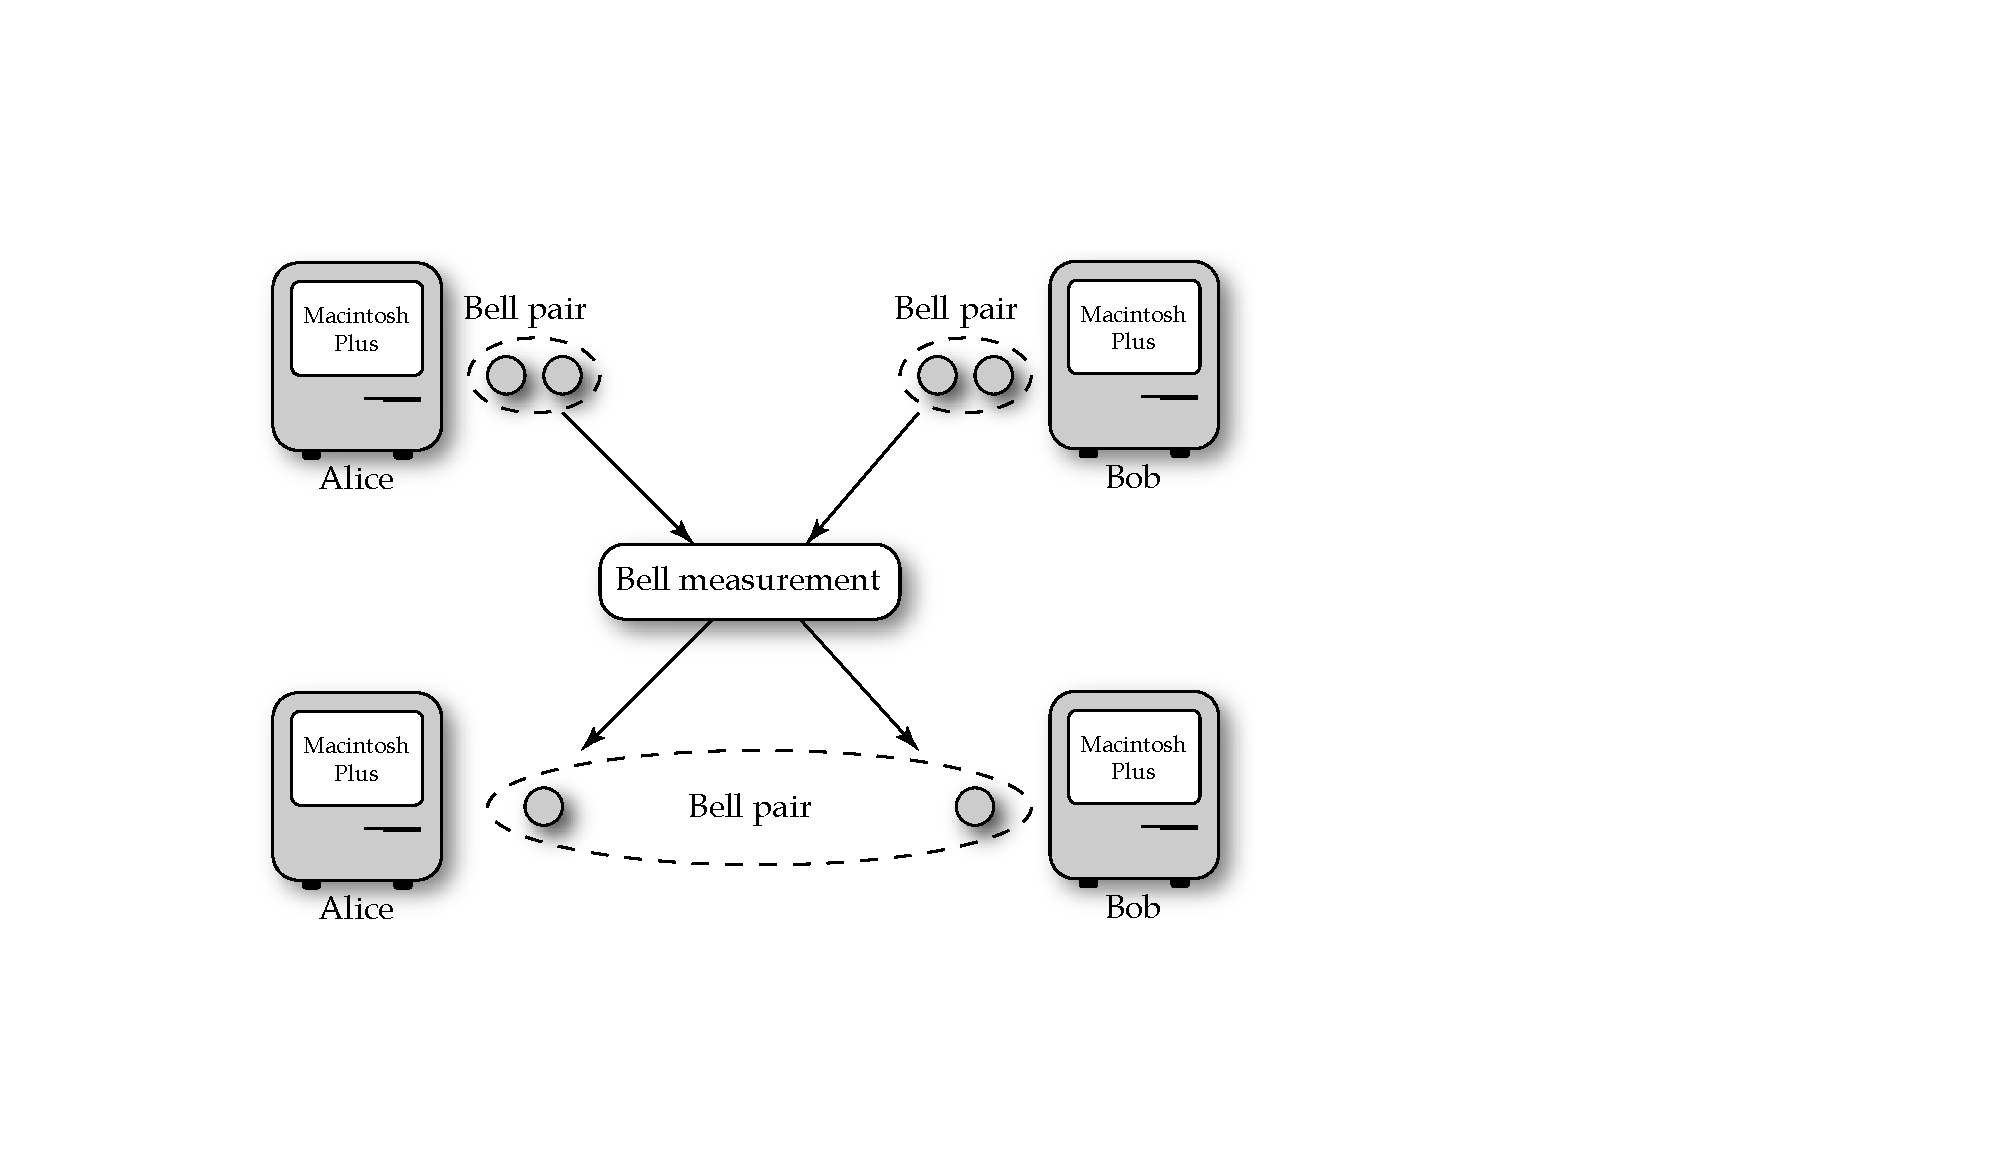
\includegraphics[width=\columnwidth]{ent_swap}
\caption{Entanglement swapping between two nodes. Each node initially holds a Bell-pair (dotted ellipses) comprising two qubits (grey circles). One qubit from each pair is sent to the repeater between them, which measures them in the Bell basis. After local unitary corrections, the two nodes share an entangled pair.} \label{fig:ent_swap}
\end{figure}

In a sense, entanglement swapping can be regarded as `indirect' entanglement distribution, whereby entanglement is created between two distant parties who do not directly exchange any quantum information.

Now if instead of Alice and Bob we have a long chain of these operations in series, then the entanglement can be swapped across the entire length of the chain, enabling the preparation of end-to-end entangled pairs, which can be employed for state teleportation.

The advantage to this approach is that the range of each repeater can be much smaller than the entire length of the channel, easing constraints imposed by errors, notably loss. Furthermore, the entanglement swapping needn't be actually performed in any chronologically linear sequence. The operations could be arbitrarily ordered, since the measurements are independent and commute. Thus, if some segments are detected as failing (e.g qubits are lost), just those segments can be performed again without requiring the entire protocol to start from scratch, unlike the na{\" i}ve direct communication technique. This `divide and conquer' approach can drastically improve performance of the network in terms of channel capacity, improving the exponential dependence of loss on distance. 

The protocol is conceptually very similar to teleportation, where instead of teleporting a qubit state, we are teleporting entanglement. Because of this similarity, it inherits similar error propagation characteristics as for teleportation discussed previously. That is, errors acting on the qubits upon which the Bell measurements are performed are effectively teleported onto the remaining qubits. Then, entanglement purification can be implemented as a higher-level layer on top of the repeaters, enabling high-fidelity entanglement distribution.

Each Bell measurement can be implemented non-deterministically using a PBS, mitigating the need for interferometric stability, as before, but therefore introducing non-determinism into the protocol.

%
% Quantum Repeater Networks
%

\subsection{Quantum repeater networks} \label{sec:rep_net}

\emph{Quantum repeaters} are devices that allow entanglement to be shared between distant nodes using a bootstrapped \emph{entanglement swapping} protocol.

\comment{Say something about the scalability of quantum repeater networks under different strategies. I believe with appropriate strategies it's possible to achieve poly rather than exp scaling. Is that right? Show details.}

\comment{For early gen repeater networks, need to know exact route - for higher level networks the route can be invisible to user.}

%
% Quantum Key Distribution (QKD)
%

\subsection{Quantum key distribution (QKD)} \label{sec:QKD}

Aside from quantum computing, a central use for quantum technologies is in cryptography \cite{bib:Gisin02}. There is only a single provably secure encryption protocol -- the \emph{one-time-pad} \cite{bib:Schneier96}. This protocol requires Alice and Bob to share a random bit-string as long as the message (plaintext) being communicated between them. The two bit-strings undergo bit-wise XOR operations to form the ciphertext. Mathematically,
\begin{align}
c = s \oplus k,
\end{align}
where $\oplus$ is the bitwise XOR operation (equivalently addition modulo 2), and $c$, $s$ and $k$ are the ciphertext, plaintext and key strings respectively, all of which are of the same length, \mbox{$|c|=|s|=|k|$}.

The security of this protocol is easy to see intuitively -- with an appropriate choice of key, \emph{any} plaintext of the same length could be inferred from the ciphertext. This means that there is no possibility of performing any kind of frequency analysis, as the ciphertext string has maximum entropy and thus no correlations. Alternately, suppose we were to try and crack this code by expressing the decryption as an oracle, where the input is a key bit-string. Then we use brute-force (or Grover's algorithm) to query the oracle for tagged elements, where by `tagged' we mean that it satisfies an appropriate test (e.g an English language test) to decide whether a decrypted message is valid. Since every possible valid plaintext can be recovered using an appropriate key, the protocol is unable to find a unique plaintext matching the ciphertext.

Importantly, the secrecy of the one-time-pad strictly requires that a key never be reused. A fresh key must be generated for each message sent, otherwise trivial frequency analysis techniques can be employed to compromise security\footnote{If the same key $k$ is used to encode two messages $s_1$ and $s_2$, yielding ciphertexts \mbox{$c_1=s_1\oplus k$} and \mbox{$c_2=s_2\oplus k$}, then we trivially obtain \mbox{$c_1 \oplus c_2 = s_1 \oplus k \oplus s_2 \oplus k = s_1 \oplus s_2$}. Now a frequency analysis on the bitwise XOR of two plaintexts can be applied, without requiring any knowledge of the key whatsoever.}.

This reduces the problem of perfect secrecy of arbitrary messages to the secrecy of shared randomness. Quantum key distribution (QKD) protocols enable this by providing a shared source of randomness between Alice and Bob, where any intercept-resend attack may be detected, guaranteed by the laws of quantum physics (specifically the Heisenberg uncertainty principle and no-cloning theorem).

The two original QKD protocols, known as the \emph{BB84} \cite{bib:BennetBrassard84}, and \emph{E91} \cite{bib:Ekert91} protocols, are based on polarisation encoding in photons. BB84 requires only the transmission of a sequence of single photons, polarisation encoded with random data. E91, on the other hand, requires a server that distributes entangled Bell-pairs between Alice and Bob. Since then, numerous other protocols for QKD have been proposed, for example, using CV states.

\begin{table}[!htb]
\fbox{\parbox{0.965\columnwidth}{\tt
function BB84():
\begin{enumerate}
\item Alice chooses a random bit $0$ or $1$.
\item Alice randomly chooses a basis, $X$ or $Z$.
\item Depending on the choice of basis, she encodes her bit into the polarisation of a single photon as:
\begin{align}
\ket{0}_Z &\equiv \ket{H}, \nonumber \\
\ket{1}_Z &\equiv \ket{V},
\end{align}
or,
\begin{align}
\ket{0}_X &\equiv \frac{1}{\sqrt{2}}(\ket{H}+\ket{V}), \nonumber \\
\ket{1}_X &\equiv \frac{1}{\sqrt{2}}(\ket{H}-\ket{V}).
\end{align}
\item Encoding into the randomly chosen basis, she transmits the randomly chosen bit to Bob.
\item She does not announce the choice of bit or basis.
\item Bob measures the bit in a randomly chosen basis, $X$ or $Z$.
\item The above is repeated many times.
\item Upon receipt of all qubits, Alice (publicly) announces the basis used for encoding each bit sent.
\item Qubits where Bob measured in the opposite basis to which Alice encoded are discarded, as they will be decorrelated from Alice.
\item The remaining measurement outcomes are guaranteed to yield identical bits between Alice and Bob.
\item Remaining is roughly half as many bits as were sent, which are random, but guaranteed to be identical between Alice and Bob.
\item Alice and Bob sacrifice some of their bits by publicly communicating them to check for consistency. This rules out intercept-resend attacks.
\end{enumerate}}}
\caption{BB84 QKD protocol using polarisation-encoded photons (or equivalently any other qubit encoding). Upon completion of the protocol, Alice and Bob share a random bit-string. Suppose an eavesdropper, Eve, were to perform an intercept-resend attack on the channel between Alice and Bob. At that stage in the protocol Alice had not yet announced her choice of bases, and Eve will not know the bases in which to measure states without randomly collapsing them onto values inconsistent with Alice's encoding. Thus, by sacrificing a small fraction of their shared bits, via openly communicating them to one another for comparison, such an intercept-resend attack will quickly be detected by Alice and Bob, with success probability exponentially asymptoting to unity. Thus, Alice and Bob have great confidence that they have a shared, secret, random bit-string, which may subsequently be employed in a one-time-pad.} \label{tab:bb84}
\end{table}

%Let us briefly consider the BB84 protocol. Alice first chooses a random basis, either $\hat{X}$ or $\hat{Z}$, in which to encode one of two randomly chosen basis states, either \mbox{$\{\ket{H},\ket{V}\}$} or \mbox{$\{\ket{+}=\frac{1}{\sqrt{2}}(\ket{H}+\ket{V}),\ket{-}=\frac{1}{\sqrt{2}}(\ket{H}-\ket{V})\}$} respectively. She sends this state to Bob, without announcing either the choice of basis or basis state. Bob subsequently measures the photon in one of the two bases, chosen randomly also. This is repeated as many times as is necessary. Finally, Bob confirms to Alice that he has received her photons, at which point she announces to him the choice of basis for each of the sent photons (this does not require secrecy). In the instances where Alice and Bob's basis choices matched, Bob has measured the same state that Alice sent, and he records the value. Otherwise he discards that sample, as it will be completely decorrelated from Alice's state, since the two measurement bases are non-commuting. What remains is approximately half as many random bits, which are guaranteed to be the same for Alice and Bob.

The BB84 protocol is described in Alg.~\ref{tab:bb84}. A key observation is that it requires no entanglement, no mode-matching, no interference, and no interferometric stability. It can be realised using nothing more than a single-photon source, wave-plates, and photo-detectors. For these reasons, QKD is a technology that is entirely viable on a large scale using present-day technology.

E91 is slightly different. Here Alice and Bob share an entangled Bell-pair provided by a central authority. Then both Alice \emph{and} Bob measure their qubits in random bases. As with BB84, after measuring all qubits, they compare their choices of random bases. When they coincide, they have a shared bit. When they don't, they discard their result. From here the remainder of the protocol is the same as for BB84.

Like BB84, E91 has no mode-matching or interferometric stability requirements, and Alice and Bob both only require single-photon detection. Unlike BB84, however, E91 requires a central authority that is able to prepare entanglement on-demand as a resource.

Importantly, unlike classical cryptographic protocols, QKD makes no assumptions about the computational complexity of inverting encoding algorithms. The protocol is information theoretically secure, and therefore no physically realisable computer, even a quantum computer, can compromise it. Thus, usual cryptanalytic techniques, like linear and differential cryptanalysis \cite{bib:Schneier96}, or the ability to factor large numbers, that are employed to attack other encryption protocols, do not compromise QKD.

It is easy to see the utility of quantum networks in enabling commodity deployment of QKD -- users desire to communicate photons across long-range ad hoc networks, with low loss and dephasing. A global quantum internet would allow quantum cryptography to truly supersede classical cryptography, bypassing the vulnerabilities faced by classical cryptography in the era of quantum computing.

QKD has been widely experimentally demonstrated over long distances \cite{bib:Muller96}, and unlike quantum computing, QKD is at the stage of commercial viability, with several vendors offering off-the-shelf plug-and-play QKD systems. Thus, a quantum internet with low cost metrics would already find substantial utility with today's technology. Currently, great progress in being made in the implementation of QKD in fibre \cite{???}, over free space \cite{bib:Buttler00}, and even over intercontinental satellite uplinks \cite{JWP}. It seems extremely likely that some government agencies would be rolling out QKD systems \cite{bib:Secret}, especially in light of the paranoia surrounding quantum codebreaking.

%
% Quantum Anonymous Broadcasting
%

\subsection{Quantum anonymous broadcasting} \label{sec:anon_broad}

\cite{Wehner}

\comment{Ryan TO DO}

%
% Superdense Coding
%

\subsection{Superdense coding}

\cite{???}

\comment{Ryan to do}

%
% Quantum Metrology
%

\subsection{Quantum metrology} \label{sec:metrology}

The goal of quantum metrology is to estimate and unknown phase with the greatest degree of precision. This finds many applications, perhaps most notably the recent gravity wave measurement protocols \cite{???}. The shot-noise limit (SNL) represents the maximum achievable precision using classical states, whereas the Heisenberg limit (HL) is the best that can be achieved using quantum resources. The goal of quantum metrology is to beat the SNL and achieve the HL.

Achieving the SNL is easily done using coherent states (Sec.~\ref{sec:coherent_states}), which are not true quantum states. However, HL metrology can be achieved using NOON states (Sec.~\ref{sec:NOON}) \cite{bib:Dowling08}. An alternate recent proposal (known as the MORDOR protocol, after the authors), employs only single-photon states (Sec.~\ref{sec:single_phot_src}) and passive linear optics, which, although not saturating the HL, significantly beats the SNL \cite{MORDOR, MORDOR2}.

Both of these types of state have their difficulties to prepare, but especially NOON states, as they cannot be deterministically prepared using linear optics, and no current source natively prepares them directly. Thus, outsourcing these state preparation stages could be of great value to end-users of metrology.

\cite{DomBerry}

%
% Quantum State & Process Tomography
%

\subsection{Quantum state \& process tomography}

In Sec.~\ref{sec:QPT} we introduced QST and QPT, as procedures by which to experimentally reconstruct unknown density matrices or process matrices respectively. It is conceivable that these tomographic procedures might want to be performed over a quantum network in a distributed fashion.

Consider the case where a node joins an existing ad hoc network. Before thinking about routing its packets through the network, it must understand the network's relevant cost metrics. Suppose that metric is one that is calculated directly from a channel's process matrix. Then, to characterise the channels in the network connecting the node to its new nearest neighbours, it could apply distributed QPT, whereby the new node is responsible for preparing the complete basis of input states required for QPT, which are transmitted to the chosen neighbour across the respective channel, after which the recipient performs all the necessary measurements in the required bases. Purely classical communication is obviously required to communicate measurement settings and outcomes.

In this simple example scenario it is immediately clear that QPT of new links in a network is perfectly suited to distributed implementation. In fact, having a node attempt to characterise a channel from start to finish could be entirely unrealistic if the channel ran over long distances -- the owner of the node would never be able to reach the other end of the channel in time for the photons' arrival!

%
% Cloud Quantum Computing
%

\section{Cloud quantum computing} \label{sec:cloud}

From the perspective of quantum computing, by far the most pressing goal for quantum networking is to facilitate \emph{cloud quantum computing}, whereby computations can be performed over a network via a client/server model. This will be of immense importance economically, allowing very expensive quantum computers to be accessible to end-users, who otherwise would have been priced out of the market. This economic model is critical to the early widespread adoption of quantum computation.

There are several protocols necessary to facilitate cloud quantum computing. First of all, we must have a means by which to remotely process data prepared by a host on a server(s). At the most basic level, this simply involves communicating quantum and/or classical data from a client to a single server for processing, which returns quantum or classical information to the client. In the most general case, a computation may be processed by multiple servers, each responsible for a different part of the computation -- \emph{distributed quantum computation}.

Many real-world applications for quantum computing will involve sensitive data, in terms of both the information being processed and the algorithms being employed. This necessitates encryption protocols allowing computations to be performed securely over a network, such that intercept-resend attacks are unable to infer the client's data, and even the host itself is unable to do so -- \emph{homomorphic encryption} and \emph{blind quantum computing}. These form the basic building blocks from which a secure cloud-based model for quantum computing may be constructed, and economic models based on the outsourcing of computations may emerge.

%
% Outsourced Computation
%

\subsection{Outsourced quantum computation}

Most simply, an outsourced computation involves Alice preparing either a quantum or classical input state, which she would like processed on Bob's computer. Bob performs the computation and returns either a quantum or classical state to Alice.

The algorithm, which Bob implements, could either be stipulated by Alice, in which case she is purely licensing Bob's hardware, or by Bob, in which case she is licensing his hardware and software. In the case of classical input and classical output, such an outsourced computation is trivial from a networking perspective, requiring no usage of the quantum network whatsoever. In the case of quantum input and/or output data, the quantum network will be required.

Despite the model being very simple, there may still be stringent requirements on the costs in the network. When the result of the computation is returned to Alice, there may be fidelity requirements. An approximate solution to a problem, or a computation with any logical errors whatsoever, may be useless, particularly for algorithms, which are not efficiently verifiable. For example, if Alice is attempting to factorise a large number using Shor's algorithm, a number of incorrect digits may make the the correct solution effectively impossible to determine. Or if a large satisfiability problem is being solved, almost any classical bit-flip errors will invalidate the result, requiring additional computation by Alice to resolve (which may be exponentially complex to perform).

In the case of classical communication of input and output data, we can reasonably assume error-free communication, owing to its digital nature. However, in the case of quantum communication it is inevitable that at least some degree of noise will be present. Depending on the application, this may require the client and host to jointly implement a distributed implementation of QEC (Secs.~\ref{sec:QOS}, \ref{sec:topol_codes}), whereby Alice and Bob communicate encoded states with one another, to which syndrome measurement and error correction are applied upon receipt. This will necessitate a limited amount of quantum processing to be directly available to Alice. In the case where she is completely starved of any quantum processing resources whatsoever, this may be a limiting factor. Otherwise, this type of cooperative QEC may be plausible.

%
% Distributed Computation
%

\subsection{Distributed quantum computation} \label{sec:dist_QC}

The elementary model described above is very limited, as many realistic data processing applications will require multiple stages of computations to be performed, potentially by different hosts. For example, a client may need data processed using multiple proprietary algorithms owned by different hosts, and the processing will need to be distributed across the network \cite{bib:Cirac99}.

There are two main models for how a distributed computation may proceed -- in \emph{parallel}, or in \emph{series} -- whereby sub-algorithms are performed either side-by-side simultaneously, or one after another in a pipeline. The two models are illustrated in Fig.~\ref{fig:distributed}.

\begin{figure}[!htb]
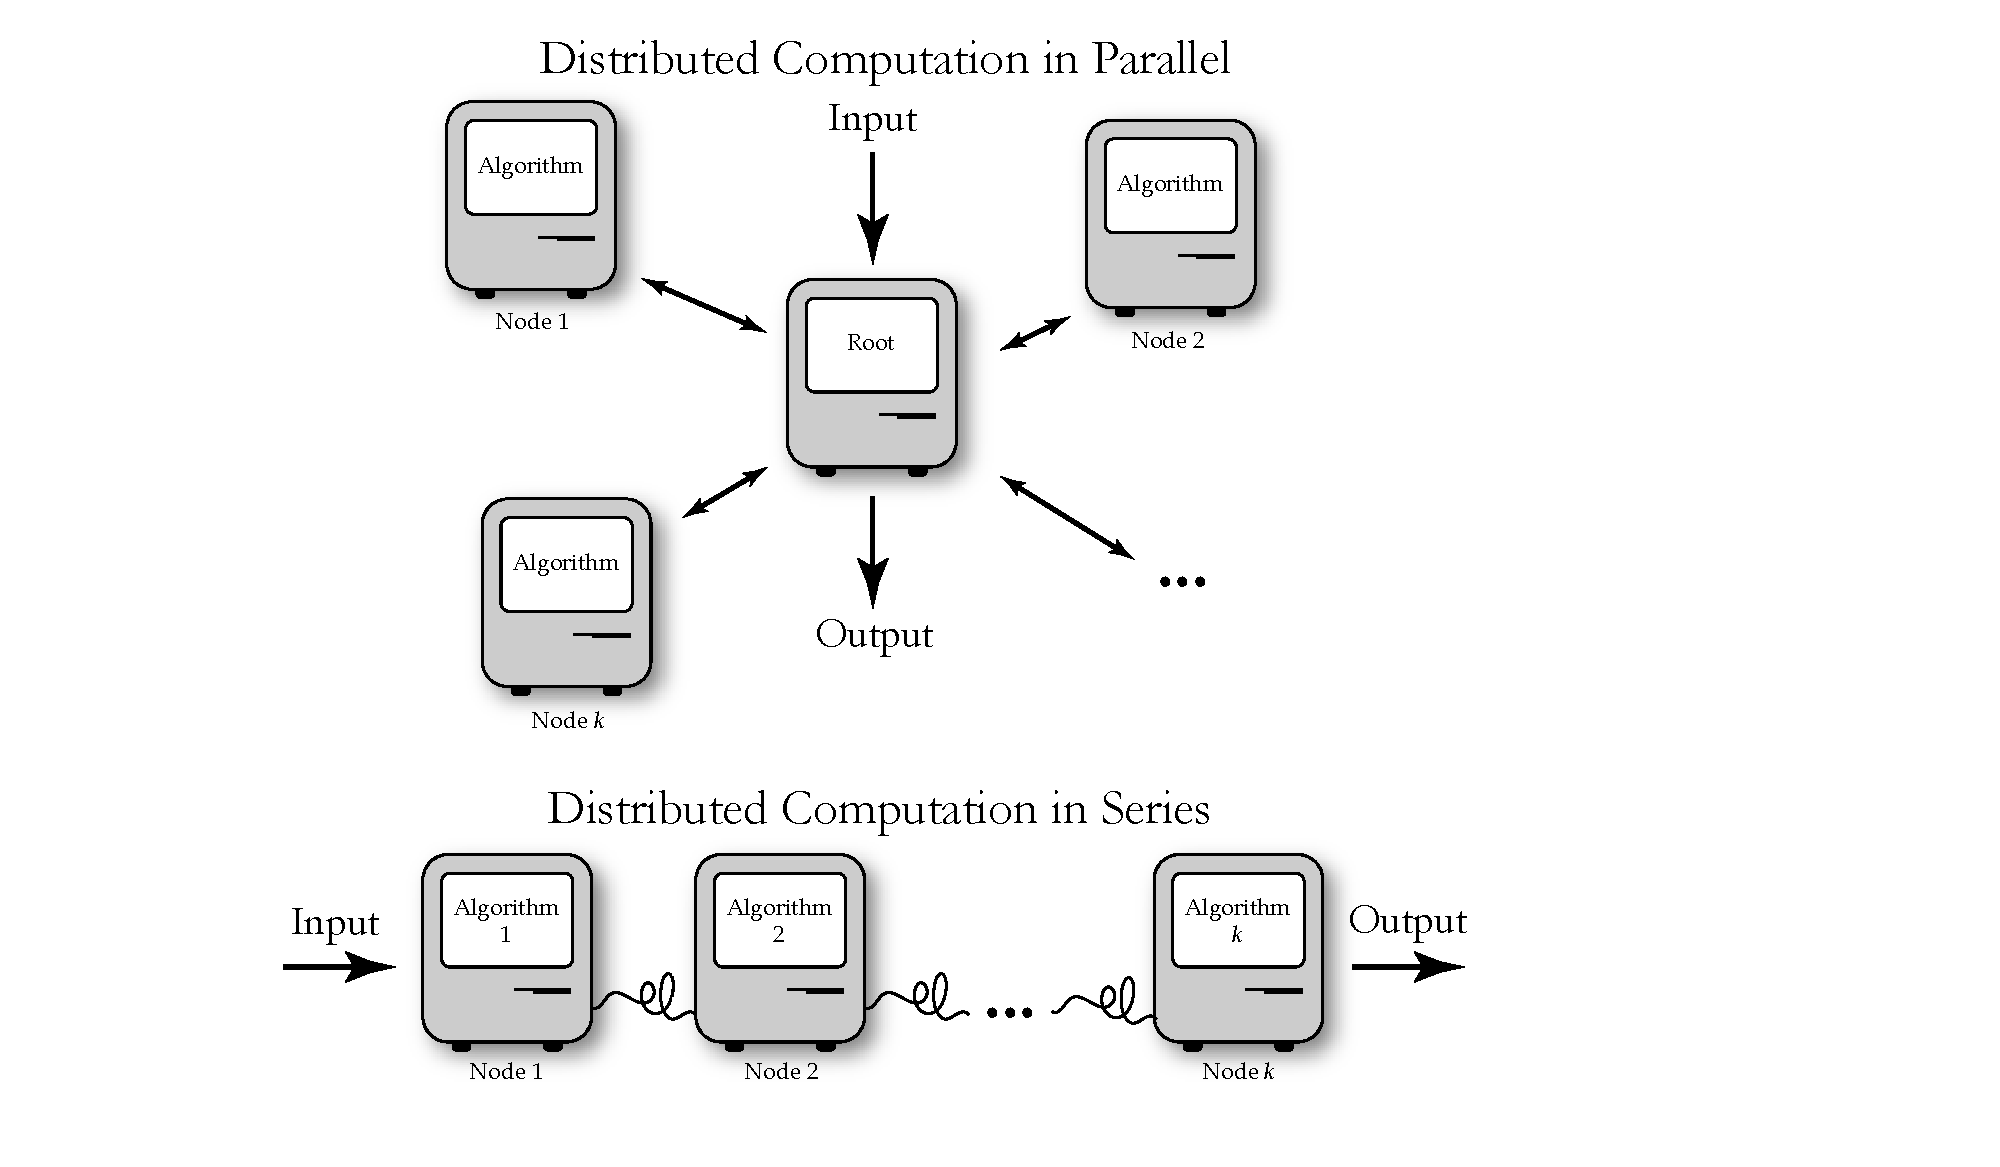
\includegraphics[width=\columnwidth]{distributed}
\caption{Models for distributed computation in parallel and in series. In parallel, a root node oversees the total computation, delegating tasks to child nodes, which process data independently of one another. In series the nodes sequentially process data in a pipeline of algorithmic stages.} \label{fig:distributed}
\end{figure}

Classical parallel processing typically involves a root node, which delegates tasks to be performed in parallel by a number of child nodes, and the results returned to the root node, which potentially applies an algorithm to merge the set of results, before returning a final result to the client. Classical models such as Google's {\sc MapReduce} protocol \cite{bib:MapReduce} are built on this idea.

In classical computing, parallel processing is widely employed to shorten algorithmic runtimes. However, the increase in clock-cycles scales only linearly with the number of nodes in the network: $k$-fold parallelisation yields a \mbox{$\sim k$}-fold speedup. For time-critical applications, such a linear improvement may be already highly beneficial, albeit costly. The attractive feature of quantum computing, however, is the potentially exponential improvement in algorithmic performance of certain tasks over their classical counterparts. This exponential relationship implies that parallelisation in general no longer has a simple linear tradeoff.

Let $t_c$ be the time required by a classical algorithm to solve a given problem, and $t_q$ the time required to solve the same problem using a quantum algorithm. In the case of algorithms exhibiting exponential quantum speedup, we will have,
\begin{align}
t_c = O(\mathrm{exp}(t_q)).
\end{align}
If we now increase the quantum processing power $k$-fold, the equivalent classical processing time is (in the best case),
\begin{align}
t_c' &= O(\mathrm{exp}(t_q k)) \nonumber \\
&= O(\mathrm{exp}(t_q)^{k}) \nonumber \\
&= O({t_c}^{k}).
\end{align}
Thus, $k$-fold quantum parallelisation corresponds to a $k$th-order exponential enhancement in the equivalent classical processing time, which clearly scales much more favourably than the linear $k$-fold enhancement offered by classical parallelisation.

The alternate scenario is in-series distributed computation, in which a computation proceeds through a pipeline of different stages, potentially performed by different hosts. This model allows a complex algorithm comprising smaller sub-routines, each of which may be proprietary with different owners, to be delegated across the network. The different stages may communicate classical and/or quantum data. As with the simple single-host model, if the different stages of the processing pipeline are sharing quantum data, distributed QEC will generally be necessary to protect the computation. This necessarily introduces an (efficient) overhead in the number of physical qubits being communicated across the network, introducing additional bandwidth costs, which must be accommodated for in networking strategies.

The cluster state (Sec.~\ref{sec:CSQC}), topological code (Sec.~\ref{sec:topol_codes}) and quantum random walk (Sec.~\ref{sec:QW}) models for quantum computation may find themselves to be particularly well-suited to distributed implementation, since they naturally reside on graphs, whose nodes needn't be held locally by a single user, but could instead be shared across multiple hosts with the ability for graph nodes to intercommunicate.

%
% Delegated Quantum Computation
%

\subsection{Delegated quantum computation}

Taking the notions of outsourced and distributed quantum computation to the logical extreme, we can envisage the situation where Alice has no quantum resources whatsoever (state preparation, evolution or measurement), but knows exactly what the processing pipeline should entail, and who on the network has the different required quantum resources. We refer to this as \emph{delegated} quantum computation, where the entire processing pipeline is outsourced to a series of hosts.

To illustrate this, let us consider a simple example -- cat state quantum computation (Sec.~\ref{sec:cat_enc}). There are three main elements to the protocol:
\begin{enumerate}
\item Cat state preparation.
\item Post-selected linear optics with feedforward.
\item Continuous variable measurement.
\end{enumerate}

Each of these stages present their own technological challenges, sufficiently challenging that one might wish to outsource all three stages. However, suppose there is no single host on the network with the ability to perform all three, but rather there are three hosts ($B_1$, $B_2$ and $B_3$), each specialising in just one of those tasks. In this instance, it would be most resource savvy for the network to implement the pipeline \mbox{$A\to B_1\to B_2\to B_3\to A$}, without going back and forth to Alice after each step (\mbox{$A\to B_1\to A\to B_2 \to A\to B_3\to A$}). In fact, it may not even be technologically possible to implement back-and-forth to Alice if she has no capacity for handling quantum resources (i.e the \mbox{$A\to B_1$} and \mbox{$B_3\to A$} stages are purely classical). An example of such a pipeline is shown in Fig.~\ref{fig:delegated}.

\begin{figure}[!htb]
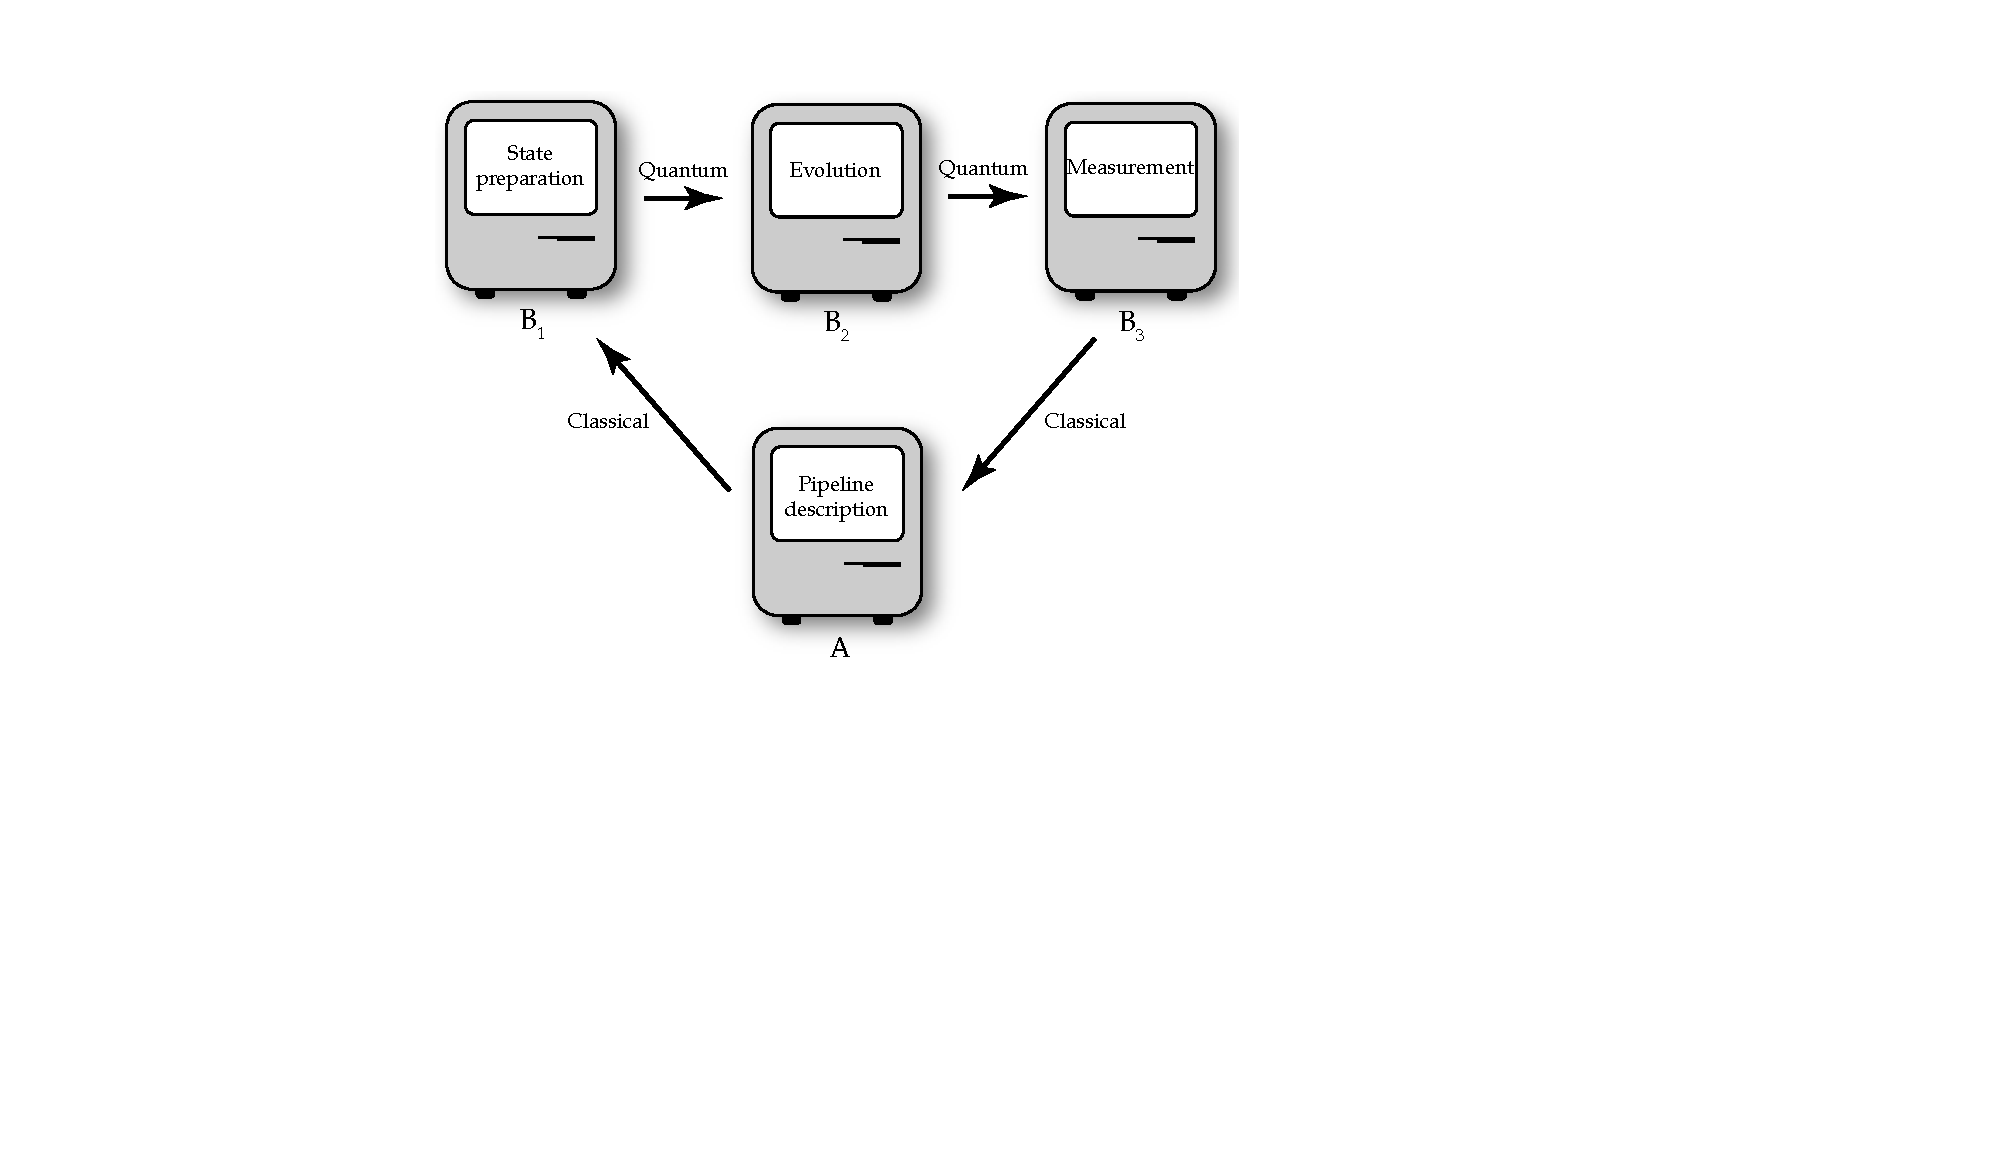
\includegraphics[width=\columnwidth]{delegated}
\caption{Delegated quantum computation, where each of the three computational stages (state preparation, evolution and measurement) are outsourced to the cloud without intermittent interaction with the client, $A$. $A$ provides only a classical description of the processing pipeline to be implemented, each stage of which is delegated to a server specialised in that particular task. Thus, the total processing pipeline takes the form \mbox{$A\to B_1\to B_2\to B_3\to A$}, where \mbox{$A\to B_1$} and \mbox{$B_3\to A$} are classical, and \mbox{$B_1\to B_2$} and \mbox{$B_2\to B_3$} are quantum channels.} \label{fig:delegated}
\end{figure}

This can be achieved by adding a {\sc Pipeline} field to the packet header prepared by Alice -- a FIFO queue describing the entire processing pipeline that Alice's packet (which initially contains only classical data) ought to follow through the network. Following completion of each stage of the pipeline we pop the stack and transmit the packet to the next specified host. Only at the very completion of the protocol is a packet (containing only classical data) returned to Alice.

Another good case study is quantum metrology using NOON states (Secs.~\ref{sec:NOON} \& \ref{sec:metrology}) for Heisenberg limited metrology. Preparing NOON states is extremely challenging, and additionally Alice may not possess the unknown phase to be measured, but rather wishes a NOON state, prepared by $B_1$, to be provided to a third party, $B_2$, who applies the unknown phase, and passes the resulting state to $B_3$, who implements the required high-efficiency parity measurements required to complete the protocol. In this case, the pipeline would take the same form as above, again with no back-and-forth communication to Alice.

Such delegated protocols will be very useful in quantum networks, where different hosts specialise in different tasks (which may be the most economically efficient model), but poor old Alice specialises in none of them, despite knowing exactly what needs to be done. This would allow an aspiring undergraduate student, who is poor (aren't they all?), to sit in his bedroom at his classical PC, and implement entire distributed quantum information processing protocols in the cloud, with no quantum resources or interactions whatsoever.

%
% Cluster States
%

\subsection{Cluster states} \label{sec:CSQC}

The \emph{circuit model} is the conventional and intuitive approach for expressing quantum algorithms, decomposing algorithms into sequences of elementary gates from a universal gate set. However, the \emph{cluster state} model for quantum computation \cite{bib:Raussendorf01, bib:Raussendorf03, bib:Nielsen06} (also referred to as the \emph{one-way}, \emph{measurement-based}, or \emph{graph state} models for quantum computation) is an extremely powerful, yet conceptually distinct paradigm, that warrants treatment of its own, owing to its significant distinction from the more familiar circuit model, and its applicability to distributed models for quantum computation.

In the cluster state model, we begin by preparing a particular, highly-entangled state, called a \emph{cluster state} or \emph{graph state}. The state is associated with a graph, $G=(V,E)$, of some topology, although rectangular lattice graphs are usually considered as they are sufficient for universal quantum computation\footnote{Note that the graph upon which a cluster state resides is not to be confused with the network graph. Rather it is just a convenient graphical representation for a class of multi-qubit states.}. That is, they act as a `substrate' for implementing arbitrary quantum computations.

In the graph, vertices represent qubits initialised into the \mbox{$\ket{+}=\frac{1}{\sqrt{2}}(\ket{0}+\ket{1})$} state, and edges represent the application of maximally entangling controlled-phase (CZ) gates, $\hat{\mathrm{CZ}}=\mathrm{diag}(1,1,1,-1)$, between vertices,
\begin{align}
\ket\psi_\mathrm{cluster} = \prod_{e\in E} \hat{\mathrm{CZ}}_e \cdot \bigotimes_{v\in V}\ket{+}_v.
\end{align}
Alternately, but equivalently, cluster states may be defined in the stabiliser formalism. Specifically, a cluster state is defined to be the joint +1 eigenstate of all the stabilisers,
\begin{align} \label{eq:CS_stab}
\hat{S}_v = \hat{X}_v \prod_{i\in n(v)} \hat{Z}_i,
\end{align}
where there is one stabiliser $\hat{S}_v$ per vertex $v$, and $n(v)$ is the set of vertices neighbouring $v$. The cluster state therefore satisfies,
\begin{align}
\hat{S}_v\ket\psi_\mathrm{cluster} = \ket\psi_\mathrm{cluster}\,\forall\, v,
\end{align}
and the full set of stabilisers $\hat{S}_v$ over all vertices $v$ is sufficient to fully characterise the cluster state, $\ket{\psi}_\mathrm{cluster}$.

An example is presented in Fig.~\ref{fig:cluster_state}. Cluster states are easily encoded optically using photonic polarisation encoding (Sec.~\ref{sec:single_phot_enc}), and therefore readily lend themselves to optical networking.

\begin{figure}[!htb]
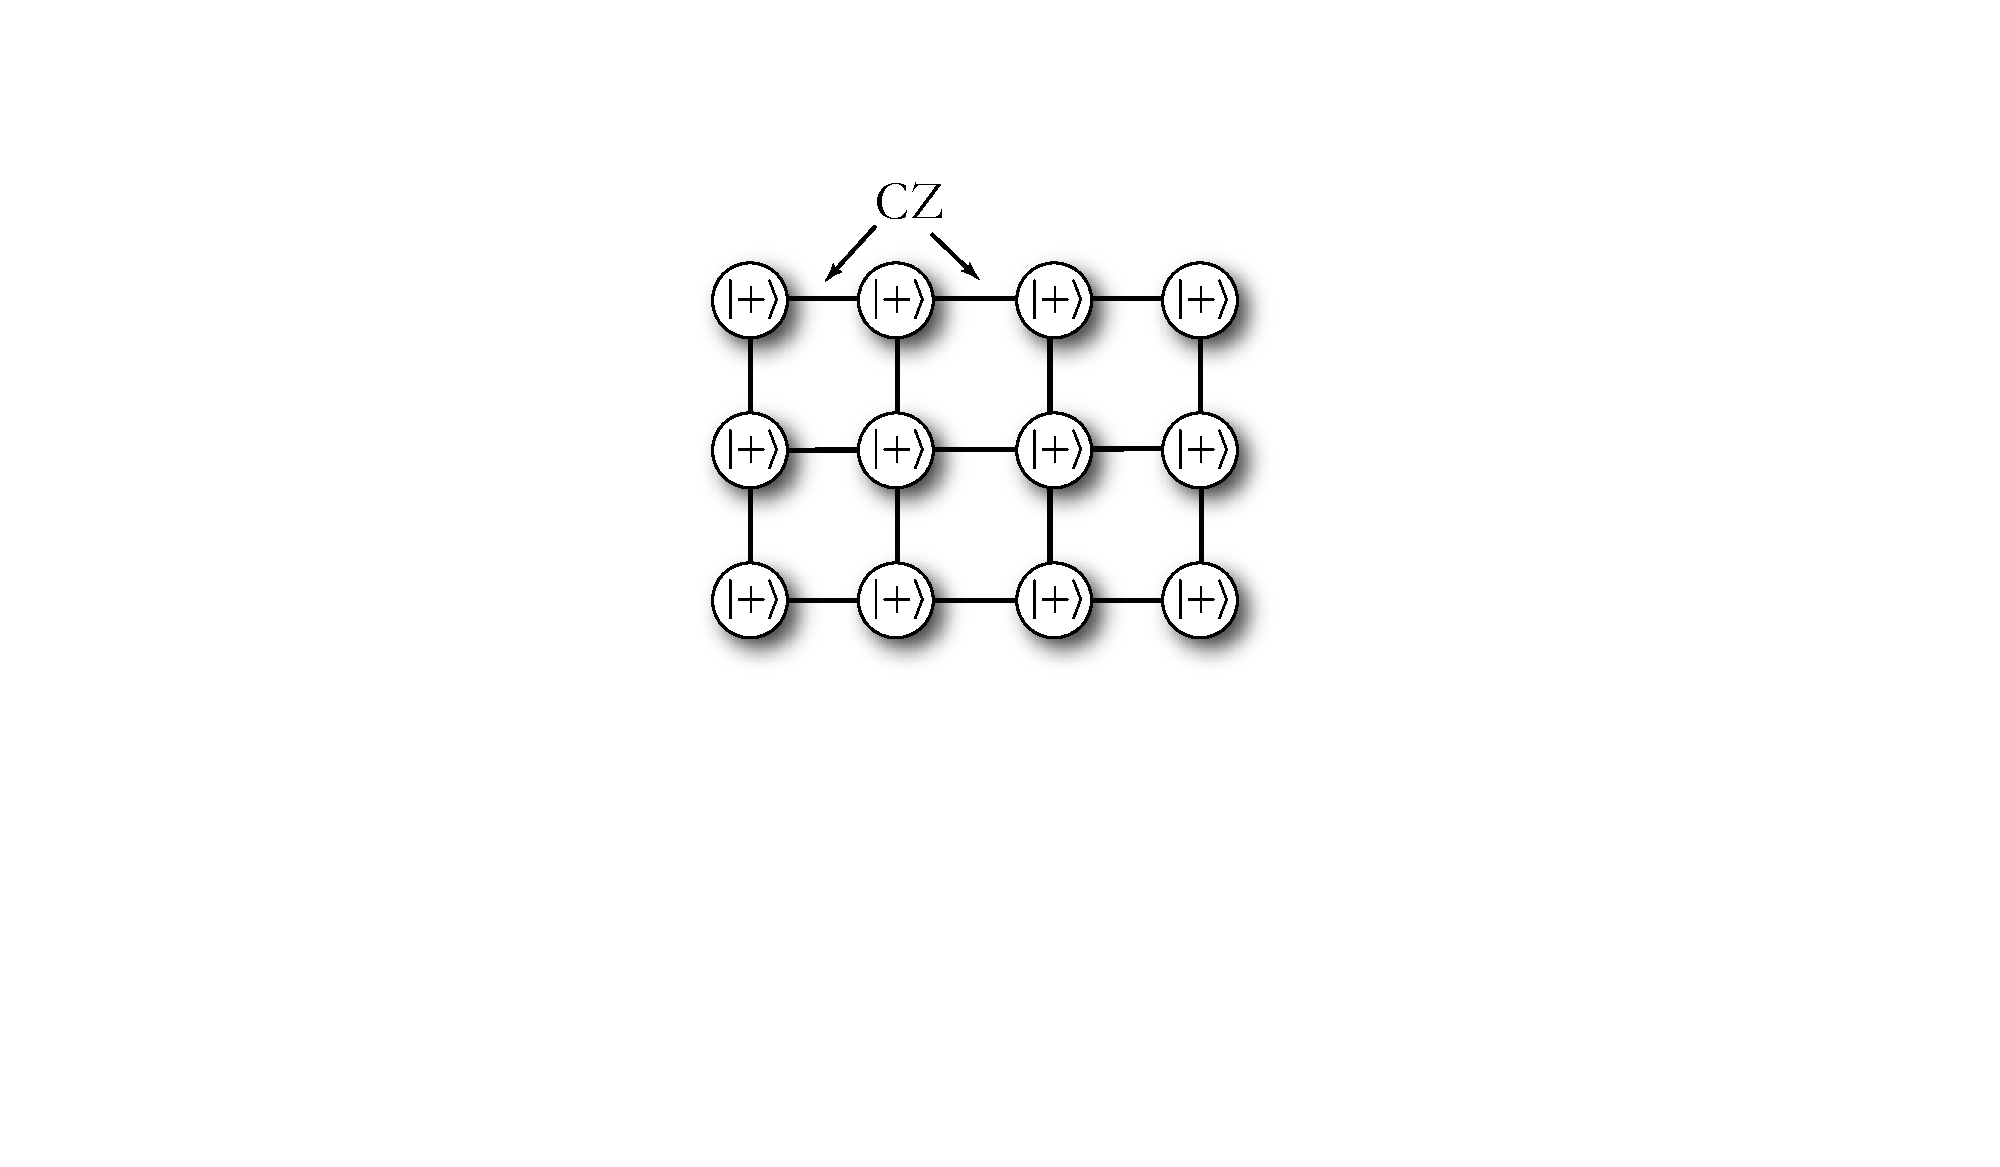
\includegraphics[width=0.6\columnwidth]{cluster_state}
\caption{Example of a \mbox{$4\times 3$} rectangular lattice cluster state. Each vertex in the graph represents a qubit initialised into \mbox{$\ket{+}=\frac{1}{\sqrt{2}}(\ket{0}+\ket{1})$}. Edges represent the application of CZ gates between qubits (CZ gates commute, so the order is unimportant). Of sufficient dimension, states of this topology enable universal measurement-based quantum computation, whereby computation proceeds purely via single-qubit measurements, and all entangling operations have been commuted to the state preparation stage. Because CZ gates commute, the preparation of cluster states is easily implemented in a distributed or parallelised manner.} \label{fig:cluster_state}
\end{figure}

Having prepared this state, the computation is implemented purely via a well-orchestrated routine of single-qubit measurements. The order and basis in which they are performed (which depends on previous measurement outcomes in general -- i.e we require fast-feedforward) then stipulates the computation. In the context of distributed computation, this requires classical communication between nodes.

It is easily shown that this model may be directly mapped to the circuit model, and is therefore universal for quantum computation.

The distinctive feature of this model is that all the entangling CZ gates are performed at the very beginning of the protocol, during the state preparation stage. The algorithm itself is purely measurement-based, requiring only single-qubit measurements (no entangling measurements).

An alternate interpretation of the cluster state model is that it is a complicated network of state and gate teleportation protocols (Sec.~\ref{sec:teleport}). Specifically, a CZ gate with a $\ket{+}$ state as a resource, followed by measurement of one of the two qubits acts as a single-qubit teleporter. Thus, the single-qubit measurements progressively teleport the input state through the graph topology, at each stage accumulating the action of more gates, which are related to the choices of the previous single-qubit measurement bases, and the graph topology.

The cluster state formalism has proven very useful, enabling the development of linear optics quantum computing (Sec.~\ref{sec:KLM_univ}) protocols, orders of magnitude more efficient than the original KLM protocol. It has been found that bonding strategies -- i.e the order in which smaller clusters are fused into larger ones when using non-deterministic gates -- plays a major role in resource overhead, and much work has been performed on efficient preparation strategies for various topologies \cite{bib:Nielsen04, bib:BarrettKok05, bib:BrowneRudolph05, bib:BenjaminEisert05, bib:Gross06, bib:RohdeStratCS07, bib:Kieling06, bib:KielingRudolphEisert06, bib:RohdeBarrett07, bib:Kieling07, bib:Campbell07, bib:Campbell07b}.

These cluster states are highly valuable, given their computational power, and the ability to communicate them from Alice, who is able to prepare them, to Bob, who lacks the technology, would be a boon for Bob.

It would be most practical, economical, and resource efficient to have a single, well-equipped server with the ability to prepare such states, who does so on behalf of everyone else, and communicates the fresh cluster states to them over the quantum internet (for a price, perhaps).

Importantly, the preparation of cluster states is readily parallelised. All the entangling CZ operations commute, the order in which they are applied is irrelevant, and a rectangular lattice cluster is completely uniform. Thus, the graphs representing smaller cluster states may be easily `fused' together to form larger cluster states using, for example, CZ gates. Several other types of entangling gates can also be employed, such as polarising beamsplitters -- so-called \emph{fusion gates} \cite{bib:BrowneRudolph05}. This allows the preparation of cluster states to be performed in a `patchwork quilt'-like manner -- a number of nodes each prepare small lattice clusters, they are all put side-by-side, and stitched together using CZ gates. This type of distributed state preparation is a perfect application for in-parallel distributed quantum processing.

Consider the scenario whereby Alice requests a large cluster state from Bob, but, while she was unable to prepare the cluster state herself, she has the technological ability to perform the measurement-based computation on the state (i.e single-qubit measurements). This would effectively bypass the need for blind/homomorphic quantum computation on Bob's hardware altogether, enabling computation with \emph{perfect} secrecy, since no foreign parties would be involved in the computation stage, and no secret data is communicated -- only the \emph{substrate} for the computation is communicated, which could be used for any purpose whatsoever. By commuting all the technologically challenging aspects of a quantum computation to the state preparation stage, we can effectively mitigate the need for blind quantum computing entirely, since the `hard work' has been done in advance by the host, and Alice gets to fulfil the computation on her own, completely bypassing poor old Bob, who was just dying to read Alice's secret love letters before processing them into Hallmark cards.

There are several cluster state identities we will utilise later, summarised in Fig.~\ref{fig:cluster_ident}.

\begin{figure}[!htb]
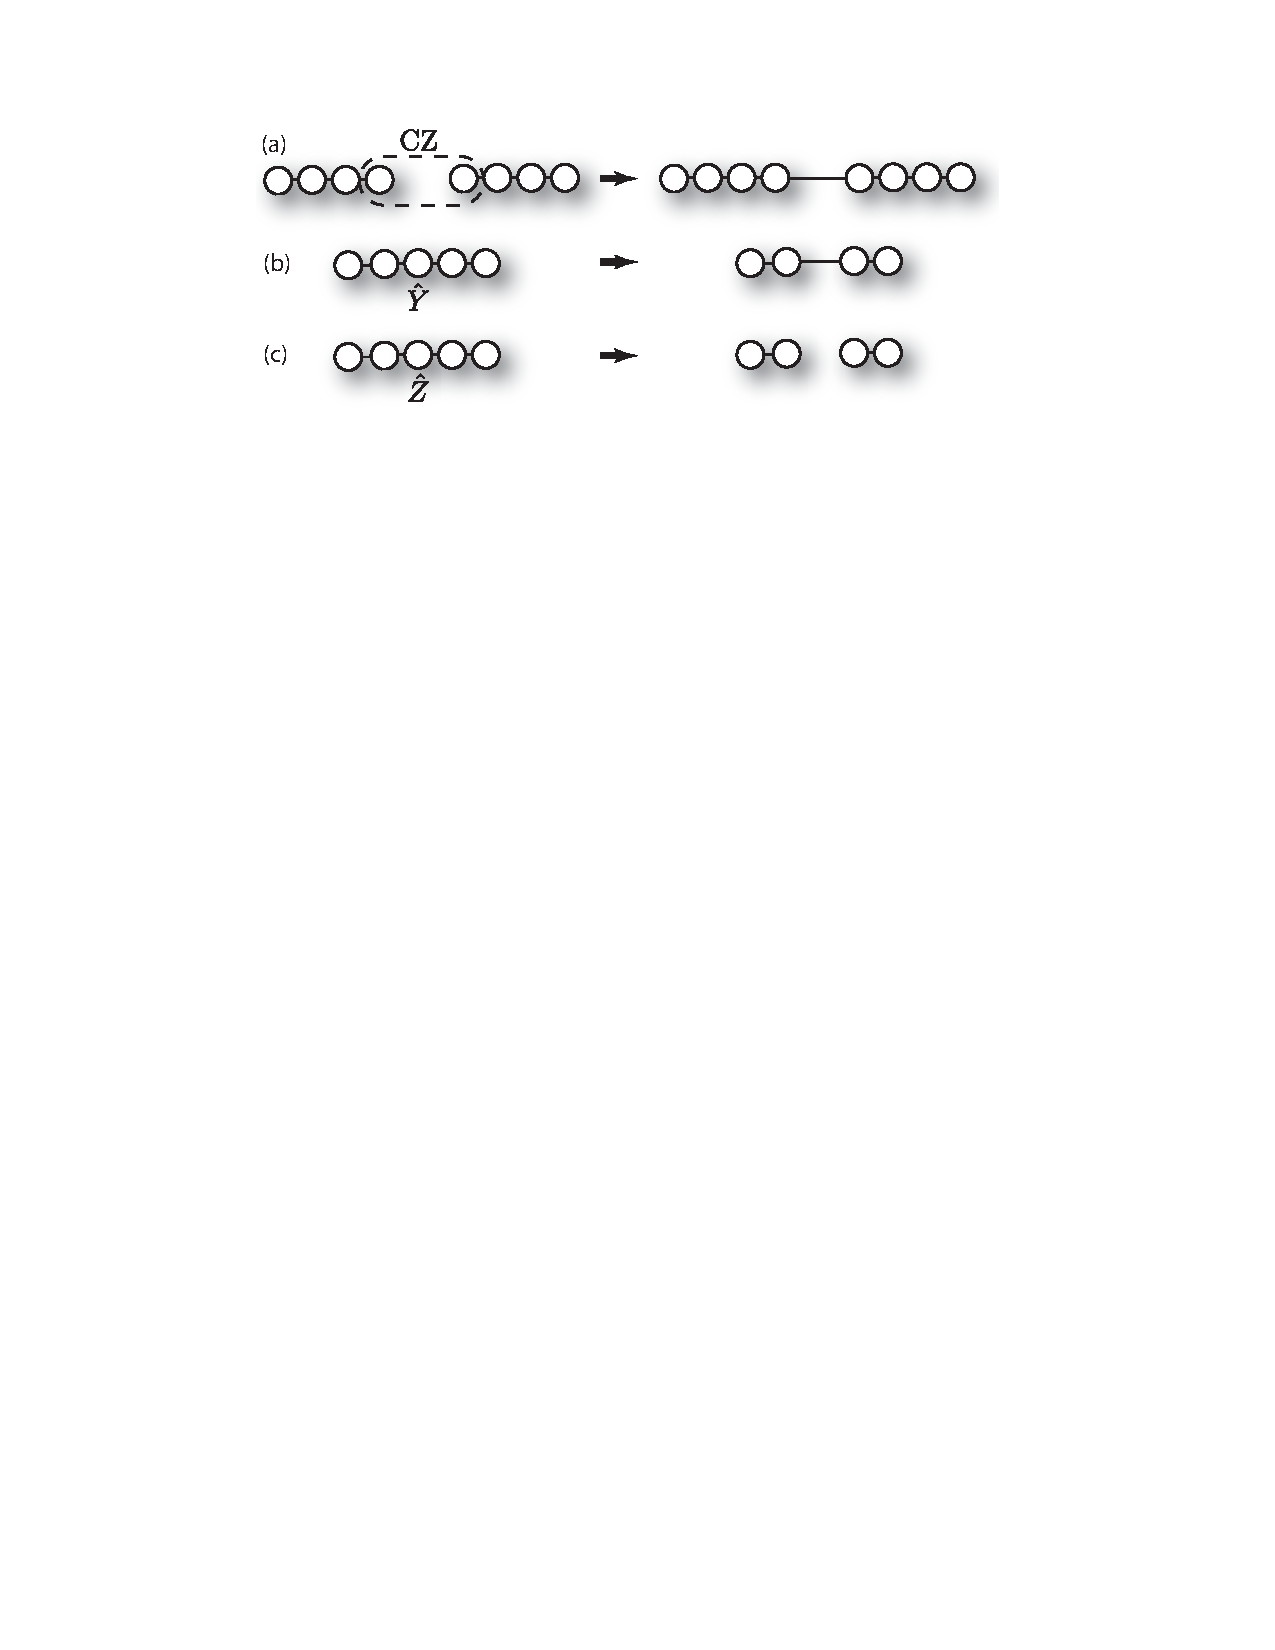
\includegraphics[width=\columnwidth]{cluster_identities}
\caption{Several cluster state identities. (a) a CZ gate between two qubits creates an edge between them in the graph. (b) Measurement of a qubit in the Pauli $\hat{Y}$ basis removes that qubit from the graph, while creating new edges between the neighbouring qubits. (c) Measurement of a qubit in the Pauli $\hat{Z}$ basis removes that qubit and any neighbouring edges.} \label{fig:cluster_ident} 
\end{figure}

When using non-deterministic gates to prepare cluster states, there are approaches to preparing ideal cluster states. This is discussed in more detail in Sec.~\ref{sec:module}. Alternately, we can borrow ideas from percolation theory to simply tolerate defects in a cluster state lattice by working around them. Specifically, if the defect probability (i.e probability of a missing vertex) is below some \emph{percolation threshold}, \mbox{$p_\mathrm{defect}\leq \epsilon_\mathrm{threshold}$}, in the asymptotic limit we are guaranteed that routes exist through the lattice. This allows defective graphs to be employed for quantum computation.

%
% Quantum Computing Using Topological Codes
%

\subsection{Quantum computing using topological codes} \label{sec:topol_codes}

If the intention is to perform quantum computations using cluster states shared over a network, QEC and fault-tolerance \emph{must} be taken into consideration, or catastrophic algorithmic failure will inevitably follow -- the cluster state model is no different from the circuit model in this respect. Fault-tolerance theory places hard thresholds on the amount of noise (typically depolarising errors and loss) qubits may be subject to in order for fault-tolerance to be possible and computations to succeed. This places strict QoS (Sec.~\ref{sec:QOS}) constraints on the network, which can be accommodated for by using the usual depolarising and efficiency cost metrics when developing networking strategies and link performance requirements.

It has been shown that fault-tolerance is possible within the cluster state model \cite{bib:NielsenDawson04, bib:Dawson06} using variations of conventional QEC codes. However, more importantly, from cluster states certain \emph{topological QEC codes} \cite{???} can be readily constructed. This implements a form of QEC-encoded measurement-based quantum computing protocol, where the computation proceeds in a measurement-based fashion, but is `natively' fault-tolerant. These codes have been shown to have very favourable fault-tolerance thresholds in terms of both depolarising noise and loss \cite{bib:StaceBarrettDohertyLoss, bib:BarrettStaceFT}, as well as frugal resource overhead compared to traditional concatenated codes. Additionally, loss- and gate-failure-tolerant codes, uniquely applicable to the cluster state model, have been described, with very favourable loss thresholds \cite{bib:Varnava05, bib:RalphHayes05, bib:Duan05}. Importantly, topological codes do not require joint measurements across the entire graph state, instead requiring only operations localised to small regions within the graph. Thanks to this, computation using such topological codes can remain distributed, without requiring the entire state to be held locally by a particular host, or requiring full access to the entire state by any particular user.

The most common topological code, which we will use here as an example, is the toric code, which resides on a lattice graph over the surface of a torus\footnote{As with cluster states, this graph needn't (but could) correspond to the network graph.}. As with cluster states (Sec.~\ref{sec:CSQC}), the toric code is most easily visualised in the stabiliser formalism. Consider a rectangular sub-graph of the torus. We place a qubit on each edge (not vertex) of the graph. Now we define two sets of stabiliser operators: \emph{star} and \emph{plaquette} operators,
\begin{align}
\hat{S}_\mathrm{star}(v) &= \prod_{i\in e(v)} \hat{X}_i, \nonumber \\
\hat{S}_\mathrm{plaquette}(p) &= \prod_{i\in e(p)} \hat{Z}_i,
\end{align}
where $e(v)$ are the edges neighbouring vertex $v$, and $e(p)$ are the edges surrounding plaquette $p$. By definition, the toric code state, $\ket\psi_\mathrm{toric}$, satisfies the stabiliser relations,
\begin{align}
\hat{S}_\mathrm{star}(v) \ket\psi_\mathrm{toric} &= \ket\psi_\mathrm{toric} \,\forall\, v, \nonumber \\
\hat{S}_\mathrm{plaquette}(p) \ket\psi_\mathrm{toric} &= \ket\psi_\mathrm{toric} \,\forall\, p.
\end{align}
Unlike the cluster state stabilisers from Eq.~\ref{eq:CS_stab}, these stabilisers are insufficient to fully characterise a unique quantum state. Rather, there are two unspecified degrees of freedom, which allows for a single qubit to be represented. Modifications of the topology, in the form of holes in the lattice (the genus of the topology), allow larger numbers of qubits to be encoded. Logical operations are implemented by performing gates and measurements across topologies over the surface.

The important feature to note is that logical qubits encoded into the toric code do not reside locally at any of the physical qubits in the code. Rather, they reside jointly across the entire graph, which, like cluster states, might be partitioned across multiple hosts, enabling distributed computation.

This is all summarised in Fig.~\ref{fig:toric_code}.

\begin{figure}[!htb]
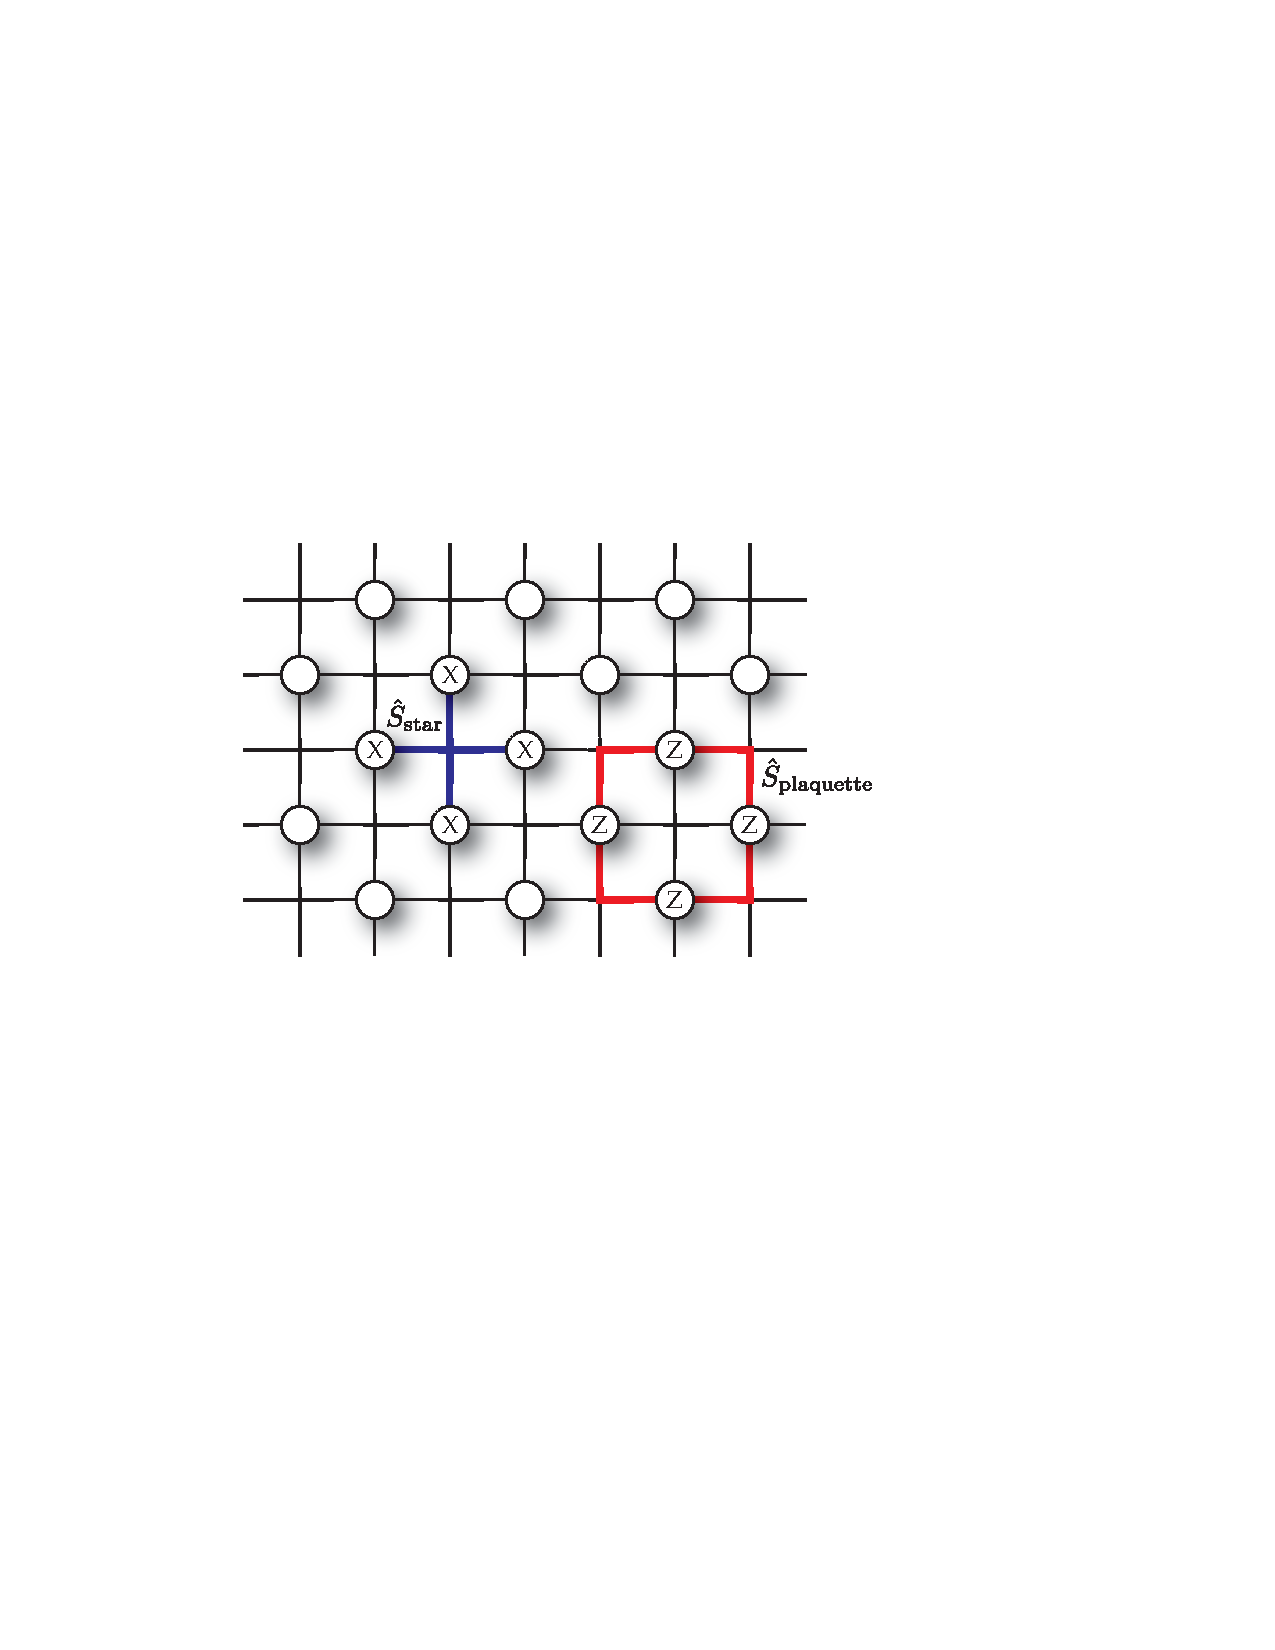
\includegraphics[width=\columnwidth]{toric_code}
\caption{Graph representation of the toric QEC code, and its associated stabilisers. The star and plaquette stabilisers across all vertices, jointly specify the state of the graph up to two missing degrees of freedom, which encode a single logical qubit. Thus, a logical qubit is encoded jointly across the entire graph, not at any specific vertex. Logical operations are performed by performing operations following topological paths through the lattice (not shown). The graph may be distributed across multiple hosts for distributed quantum computation.} \label{fig:toric_code}
\end{figure}

\comment{How to convert cluster states to topological codes. Add pic of surface code stabilisers, showing localisation of operations.}

Having defined the toric code as such, QEC proceeds in a similar manner to any other stabiliser code -- we measure all the stabilisers, yielding a syndrome, from which we can determine geometrically where errors took place in the graph, which can subsequently be corrected (if below threshold). Importantly, the stabilisers are all defined over geometrically localised neighbourhood regions, and do not require long-range measurements, making this type of code suitable to distributed models for quantum computation.

\comment{What about the actual computation? Can this still be distributed when we do the topological gates etc?}

%
% Universal Linear Optics Quantum Computing
%

\subsection{Universal linear optics} \label{sec:KLM_univ}

With single-photon encoding of qubits in the quantum network, the obvious architecture to implement quantum computation is linear optics quantum computing (LOQC) \cite{bib:KLM01} (KLM), since the states being processed by the computer are of the same form as the states traversing the network. See \cite{bib:Kok05, bib:KokLovettBook} for excellent introductions to this what has become a very broad and exciting field.

LOQC allows universal quantum computing to be implemented using single-photon polarisation or dual-rail encoding, with only linear optics interactions, i.e beamsplitter/phase-shifter networks \cite{bib:Reck94}, with the addition of quantum memory, and fast-feedforward, whereby some photons are measured, and the remaining part of the optical circuit is dynamically reconfigured based on the measurement outcomes. The former is readily available technology today, and elementary demonstrations have been performed \cite{bib:OBrien03, bib:UniversalLOOBrien}, but the latter two have proven to be somewhat more challenging.

Originally it was believed that universal optical quantum computation, specifically the implementation of two-qubit entangling gates (such as CNOT or CZ gates), would require extremely (and unrealistically) strong optical non-linearities that implement a non-linear sign-shift (NS) gate,
\begin{align} \label{eq:NS_trans}
NS: \alpha\ket{0}+\beta\ket{1}+\gamma\ket{2}\to\alpha\ket{0}+\beta\ket{1}-\gamma\ket{2},
\end{align}
in the photon-number basis, up to normalisation (which is determined by the post-selection success probability). That is, it applies a $\pi$ phase-shift to only the $\ket{2}$ component of a photon-number superposition. The breakthrough result by KLM demonstrated that this is in fact not the case at all. Instead, the NS gate can be implemented non-deterministically using post-selected linear optics. Two such NS gates allow the construction of a single CZ gate. The construction of the KLM NS and CZ gates are shown in Fig.~\ref{fig:KLM_gate}.

\begin{figure}[!htb]
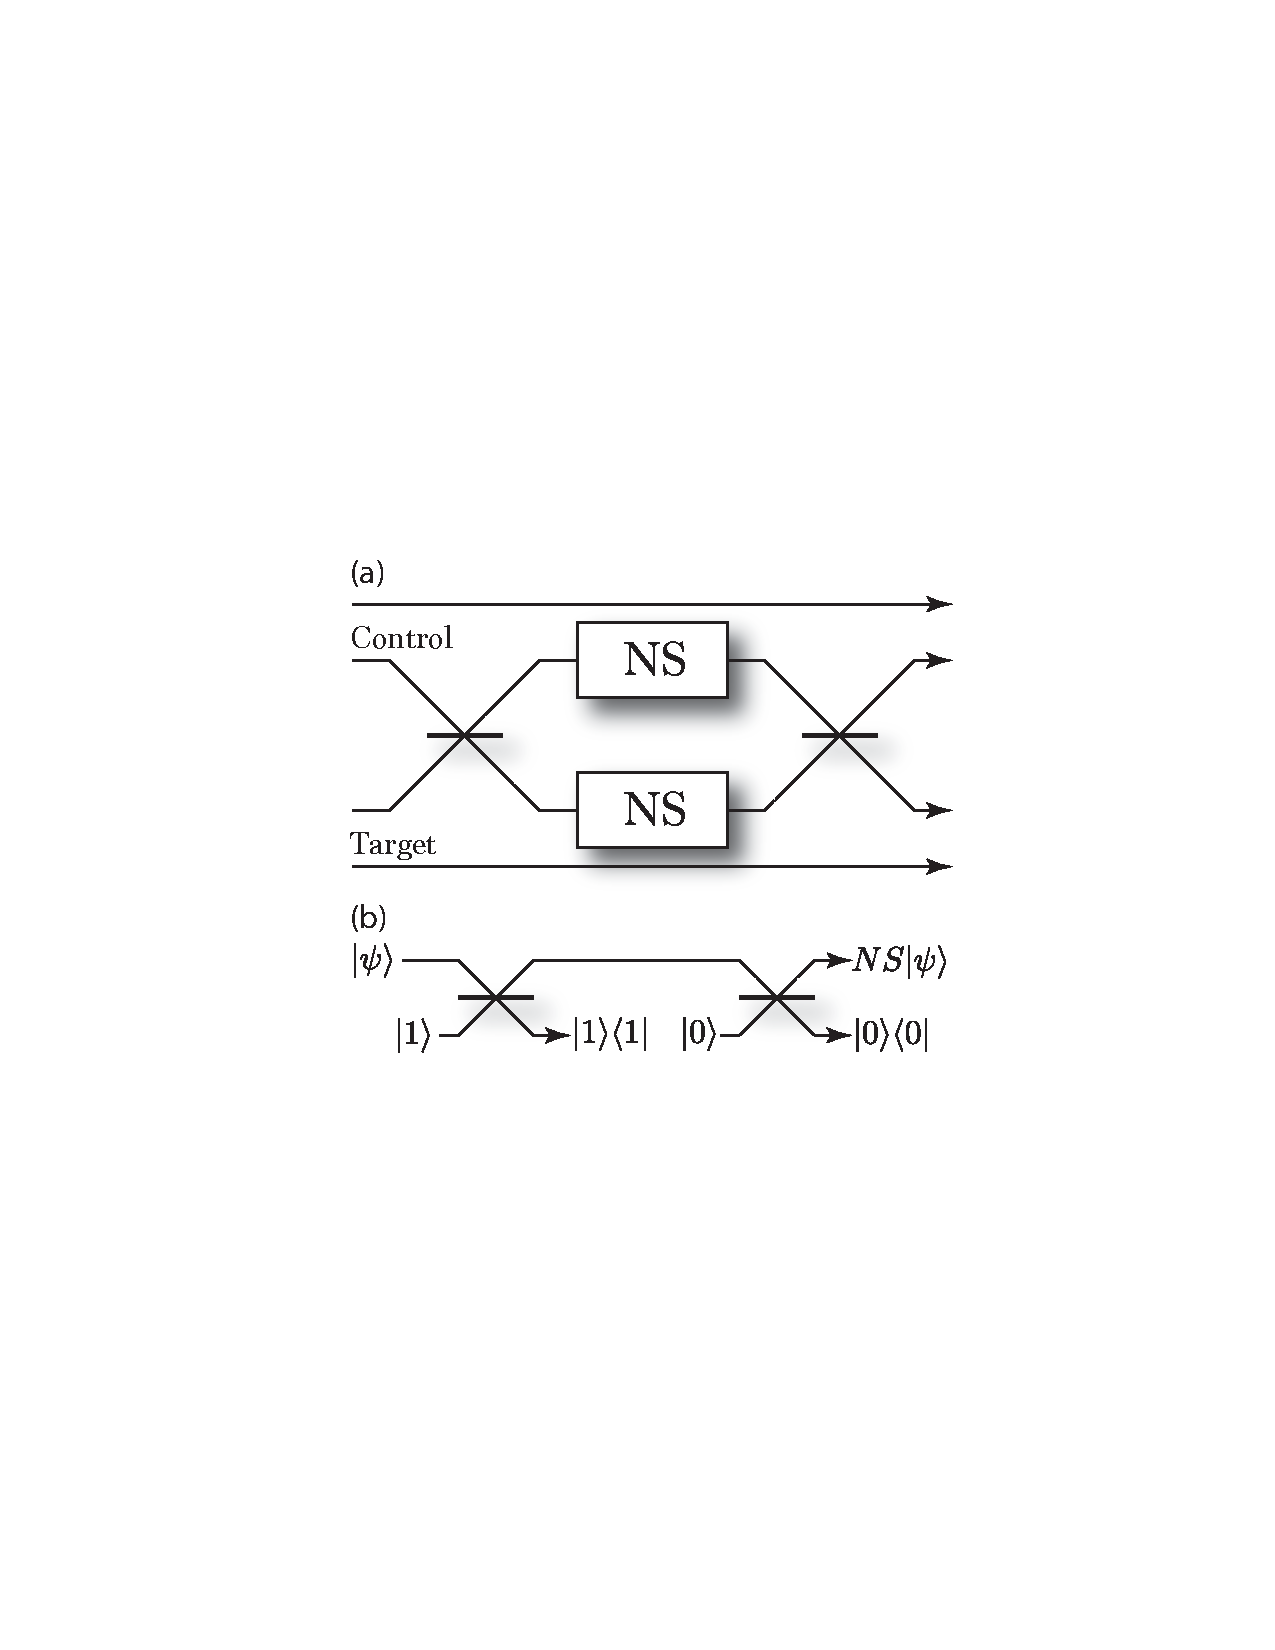
\includegraphics[width=0.8\columnwidth]{KLM_gate}
\caption{(a) A KLM CZ gate, employing dual-rail encoding, constructed from two non-linear sign-shift (NS) gates, which apply a $\pi$ phase-shift to only $\ket{2}$ terms in the photon-number basis. NS gates could be constructed using extremely (impractically) strong non-linearities. However, they can be implemented non-deterministically using two beamsplitters, two ancillary states, and two photo-detectors, post-selecting upon detecting $\ket{1}\bra{1}$ and $\ket{0}\bra{0}$ respectively. (b) Construction of the non-deterministic linear optics NS gate. Two ancillary states -- one $\ket{1}$ and one $\ket{0}$ -- are employed, and two photo-detectors post-select upon detecting $\ket{1}\bra{1}$ and $\ket{0}\bra{0}$ respectively. The beamsplitter reflectivities in (a) are 50:50, and in (b) are chosen such that the amplitudes obey Eq.~\ref{eq:NS_trans}.}. \label{fig:KLM_gate}
\end{figure}

Clearly this non-determinism is of immediate concern, since concatenating multiple gates would have exponentially decreasing success probability, making the protocol inefficient -- if the probability of a single gate succeeding is $p$, and we require that a circuit comprising $n$ of them all succeed, the success probability is clearly $p^n$.

The first key observation then is that gate teleportation can be used to shift this non-determinism to a resource state preparation stage, as described in detail in Sec.~\ref{sec:teleport_gate}. However, this is not the end of the story, since gate teleportation requires Bell state projections, which are themselves non-deterministic using purely linear optics (either using PBS's or CNOT gates).

The final insight provided by KLM is that by concatenating these non-deterministic CNOT gates, we can inductively build up higher-level CNOT gates with ever increasing success probabilities, asymptoting to unity with high-depth (but polynomial) concatenation. By combining these key insights, KLM were able to show that near-deterministic CNOT gates can be constructed using an efficient resource overhead, thereby enabling efficient universal quantum computation\footnote{Note that all single-qubit gates are trivially and deterministically implemented using wave-plates or beamsplitters, for polarisation or dual-rail encoding respectively. Thus, we need only concern ourselves with the challenges associated with implementing two-qubit entangling gates.}. A sketch of the general KLM formalism is shown in Fig.~\ref{fig:KLM_protocol}.

\begin{figure}[!htb]
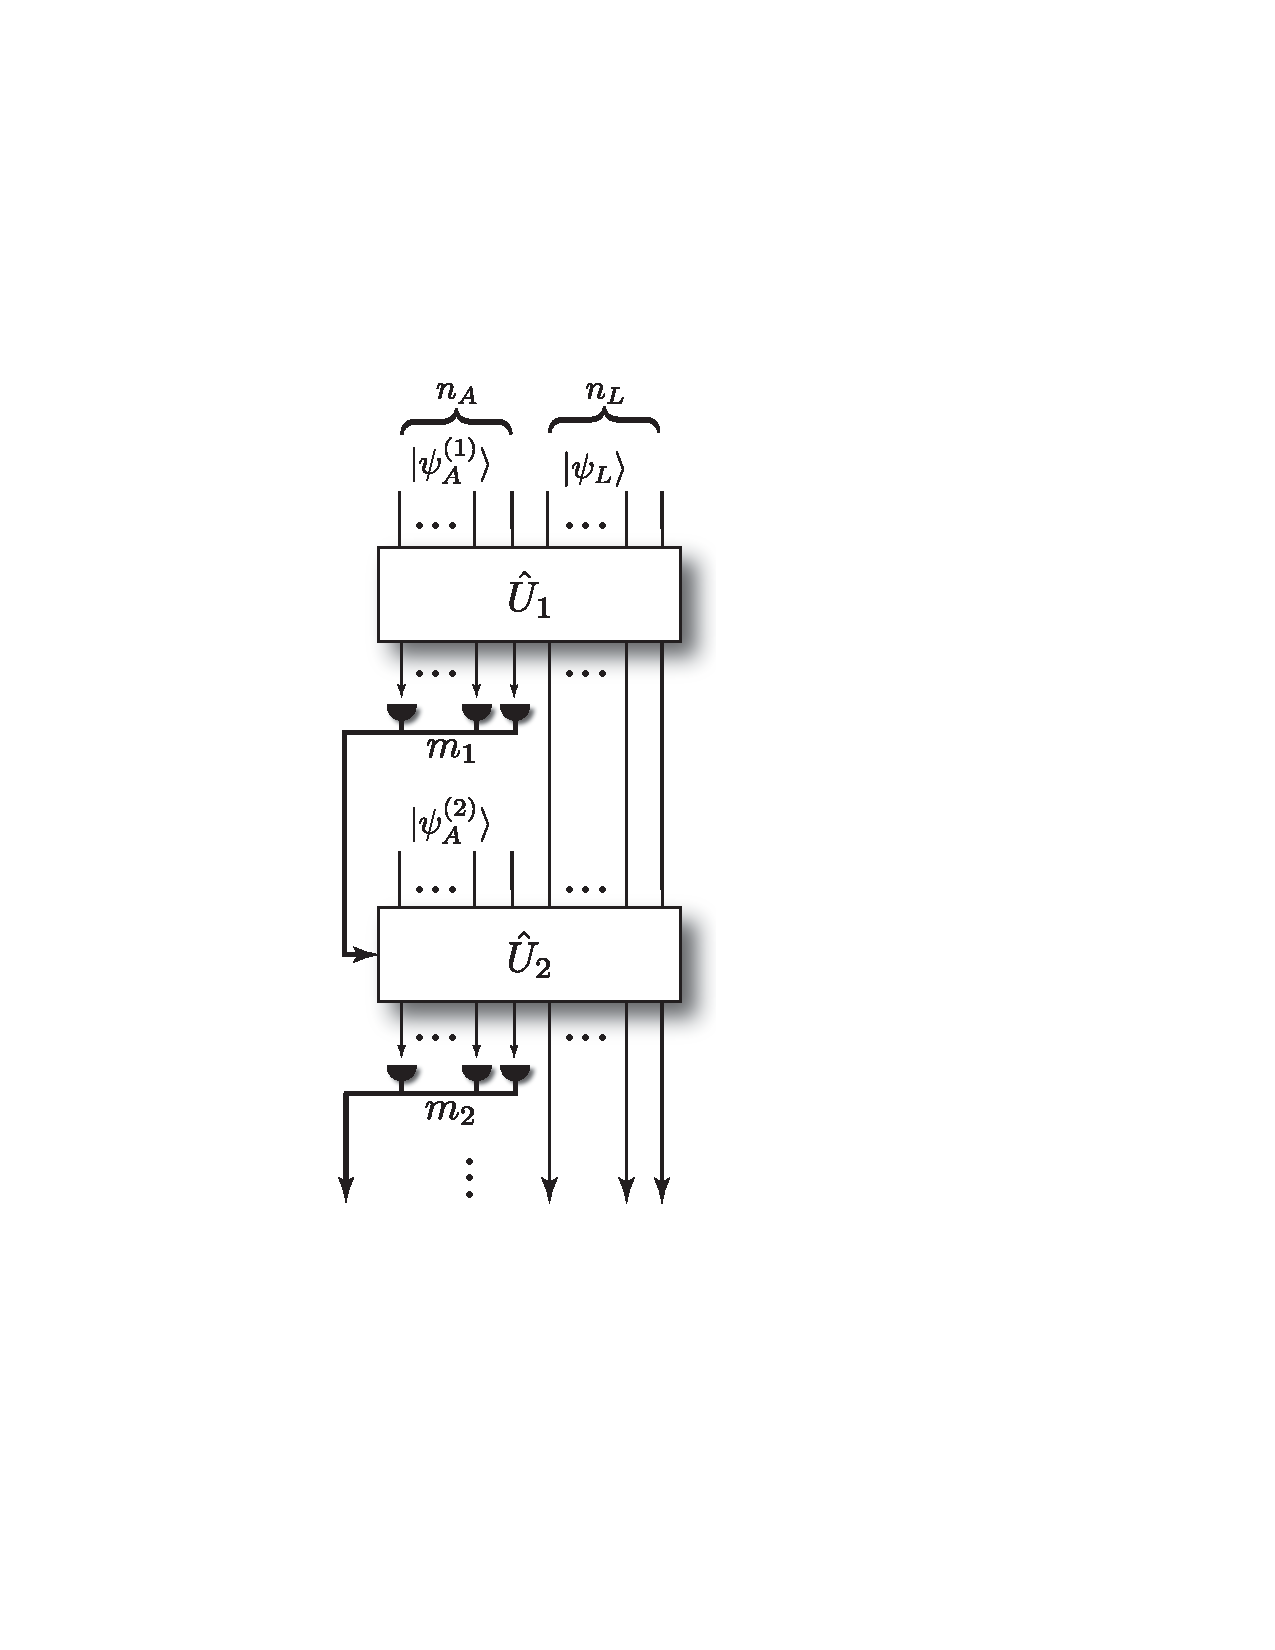
\includegraphics[width=0.5\columnwidth]{KLM}
\caption{KLM architecture for universal LOQC. $n_L$ optical modes are associated with logical qubits in the state $\ket{\psi_L}$, with the remaining $n_A$ modes acting as ancillary states, $\ket{\psi_A}$. A round of passive linear optics is applied, $\hat{U}_1$. Then the ancillary modes are measured, yielding some set of measurement outcomes $m_1$. These are classically processed to determine what the next round of passive linear optics, $\hat{U}_2$, ought to be. This repeats some polynomial number of times, from which an arbitrary quantum computation can be implemented. The {\sc BosonSampling} and quantum walk models are equivalent to taking just the first stage of this protocol: one round of input state, passive linear optics, and measurement.} \label{fig:KLM_protocol}
\end{figure}

The unitary linear optics networks implement linear maps of the form,
\begin{align} \label{sec:LO_unitary_map}
\hat{U}\hat{a}_i^\dag \hat{U}^\dag \to \sum_{j=1}^m U_{i,j} \hat{a}^\dag_j,
\end{align}
where $\hat{a}^\dag_i$ is the photonic creation operator on the $i$th of the $m$ modes, and $U$ may be any $\mathrm{SU}(m)$ matrix. These linear optics evolutions are most commonly implemented using either:
\begin{itemize}
\item Bulk optics: where discrete optical elements are arranged on an optical table.
\item Integrated waveguides: where all passive components are etched into a chip.
\item Time-bin architectures: where time-bin encoded qubits (Sec.~\ref{sec:time_bin}) evolve through delay lines and interfere at a single central optical component.
\end{itemize}
These are described in more detail in Sec.~\ref{sec:LO_evolution}.

The measurements are implemented simply by number-resolved photo-detectors, implementing measurement projectors of the form \mbox{$\hat\Pi_n=\ket{n}\bra{n}$}, for the measurement outcome of $n$ photons (Sec.~\ref{sec:photo_detection}).

Since the original presentation of a universal LOQC gate set by KLM, numerous alternate implementations have been presented and experimentally demonstrated, with various pros and cons \cite{bib:Ralph01, bib:Pittman01, bib:Ralph02, bib:Knill02, bib:Pittman03, bib:MorYoran06}.

Although the original KLM scheme is universal, resource usage can be reduced by orders of magnitude by combining concepts from LOQC with the cluster state formalism (Sec.~\ref{sec:CSQC}) or related concepts \cite{bib:YoranReznik03, bib:Nielsen04, bib:BrowneRudolph05, bib:GilchristHayes05, bib:Lim05, bib:LimBarrett05}.

Significant progress is being made on reconfigurable, integrated LOQC devices \cite{bib:UniversalLOOBrien}, but switching times remain orders of magnitude slower than that required for fast-feedforward. The resource overhead associated with overcoming the non-determinism of entangling gates is substantial in the original KLM proposal. But despite being improved upon by cluster state approaches, resource scaling remains daunting. It therefore seems most likely that certain elements from LOQC might be combined into hybrid architectures, to be discussed in detail in Sec.~\ref{sec:hybrid}.

More recently, it was shown that by introducing strong coherent states, the strength of a cross-Kerr optical non-linearity can be effectively amplified, allowing even very weak non-linearities to be employed for deterministic entangling gate operations \cite{bib:Munro05}. However, such schemes are particularly sensitive to loss, and LOQC appears more technologically viable.

%
% Passive Linear Optics
%

\subsection{Passive linear optics} \label{sec:passive_LO}

While the KLM protocol (and subsequent improvements, e.g using cluster states) are universal for quantum computing, some of the key technological requirements are very challenging, and unlikely to be achieved in the short-term. However, simplified yet non-universal models for optical quantum computing can abandon some of the more challenging requirements, nonetheless implementing a restricted set of post-classical quantum computations. In particular, we consider protocols requiring only photon-number state preparation, passive linear optics evolution (as per Eq.~\ref{sec:LO_unitary_map}), and photo-detection.

Optically, the two main contenders for this are multi-photon quantum walks \cite{bib:Aharonov93, bib:Aharonov01, bib:Kempe03, bib:Salvador12, bib:RohdeMultiWalk11} and {\sc BosonSampling} \cite{bib:AaronsonArkhipov10, bib:RohdeIntroBS15}, both closely related in that they require only passive linear optics and single-photon states, whilst mitigating the need for active switching, quantum memory and dynamic fast-feedforward. Since, evidence has been presented that similar passive linear optics protocols may implement computationally hard problems using states of light other than photon-number states \cite{bib:RandBS, bib:RohdePhotAdd15, bib:RohdeDisp15, bib:RohdeCat15}.

These protocols involve nothing more than evolving multiple single-photon states through beamsplitter networks and measuring the output photo-statistics. This is equivalent to just taking the first stage of the KLM protocol shown in Fig.~\ref{fig:KLM_protocol}.

Both quantum walks and {\sc BosonSampling} have been subject to extensive experimental investigation in recent years \cite{bib:PeruzzoQW, bib:Broome10, bib:Schreiber11b, bib:Owens11, bib:RohdeQWExp12, bib:Broome2012, bib:RohdeQWExp12, bib:Spring2, bib:Crespi3, bib:Tillmann4}.

Because these models are entirely passive, they can be made cloud-based very trivially: Alice prepares her permutation of single photons as the input state, sends it to Bob over the quantum network, who applies the passive operations before returning the state to Alice. In this case, no intermediate client/server interaction is required. Alternately, she could classically communicate a bit-string to Bob indicating the input photon-number configuration, in case she is unable to prepare it herself.

%
% Boson-Sampling
%

\subsubsection{Boson-sampling} \label{sec:BS}

{\sc BosonSampling} is the problem of sampling the output photon-number statistics of a linear optics interferometer fed with single-photon inputs. While not universal for quantum computing (in fact no one has any idea what to use it for at all!), there is strong evidence that it is a classically hard problem \cite{bib:AaronsonArkhipov10}.

The computational hardness of {\sc BosonSampling} relates to the fact that the amplitudes in the output superpositions are proportional to matrix permanents, which are known to be \#\textbf{P}-hard in general. This is believed to be a classically hard complexity class, even harder than \textbf{NP}-complete in the complexity hierarchy, requiring exponential classical time to evaluate. This yields computationally complex sampling problems.

Specifically, for an $m$-mode interferometer, and input state,
\begin{align}
\ket\psi_\mathrm{in} = \ket{T_1,\dots,T_m},
\end{align}
where there are $T_i$ photons in the $i$th input mode, the output superposition takes the form,
\begin{align}
\ket\psi_\mathrm{out} = \sum_S \gamma_{S,T} \ket{S_1,\dots,S_m},
\end{align}
where $S$ sums over all possible photon-number configurations at the output, of which there are,
\begin{align}
|S| = \binom{n+m-1}{n}.
\end{align}

The amplitudes $\gamma_{S,T}$ are given by,
\begin{align}
\gamma_{S,T} = \frac{\mathrm{Per}(U_{S,T})}{\sqrt{S_1!\dots S_m! T_1!\dots T_m!}},
\end{align}
where $\mathrm{Per}(\cdot)$ denotes the matrix permanent, and $U_{S,T}$ is a sub-matrix of $U$, obtained by taking $S_i$ copies of the $i$th row, and $T_j$ copies of the $j$th column of the linear optics unitary matrix $U$. The probability of measuring a given configuration is obviously \mbox{$P_{S,T} = |\gamma_{S,T}|^2$}.

In the case of {\sc BosonSampling}, the unitary is chosen randomly from the Haar-measure\footnote{The Haar-measure generalises the notion of a uniform distribution to higher-dimensional topologies than the real numbers, in this case to the $\mathrm{SU}(n)$ group.}.

%
% Quantum Walks
%

\subsubsection{Quantum walks} \label{sec:QW}

Photonic quantum walks (QW's) are the other contender for implementing restricted quantum computation, without requiring the full spectrum of challenging LOQC operations. The resource requirements are the same as for {\sc BosonSampling}, the difference being that now instead of choosing a Haar-random unitary matrix for the interferometer, we choose one which encodes a graph. The photons are now referred to as `walkers', and they evolve by following edges within the graph, `hopping' between neighbouring vertices.

With only a single walker (photon), nothing computationally complex can occur in the system, since a single photon evolving under passive linear optics can be efficiently classically simulated. However, once multiple walkers are introduced we have a system with almost identical features to {\sc BosonSampling}, differing only in the structure of the linear optics unitary.

There are two predominant varieties of quantum walks: discrete-time and continuous-time. In the discrete-time QW model, each walker has access to an ancillary `coin' Hilbert space, which is used to record the direction of the walker through the graph. At each discrete time-step the coin is used to update the position (vertex) of the walker, before applying a unitary `coin' operator to the coin Hilbert space. The addition of the coin space is necessary to enable such quantum walks to reside on arbitrary graph topologies, whilst retaining unitarity in their evolution. In the continuous-time QW model, on the other hand, there is no coin degree of freedom, and a Hamiltonian encoding the graph structure of the QW evolves the walker(s).

Algorithms have been described for both the discrete- and continuous-time QW models.

%
% Continuous Variables
%

\subsection{Continuous variables}

\comment{TO DO}

Sec.~\ref{sec:CV_enc}
\cite{bib:Menicucci06, lund, ralph, weedbrook}
Cat states
Gaussian states

%
% Hybrid Architectures
%

\subsection{Hybrid architectures} \label{sec:hybrid}

It is unlikely that future, large-scale quantum computers will be purely optical. Some other technologies have a more favourable outlook in terms of scalability. Nonetheless, when it comes to networking quantum computers, optics is the natural approach, motivating investigation of hybrid architectures, where qubits are represented using some non-optical system, but entangling operations between them are mediated by optical states \cite{bib:Duan06, bib:Beugnon06}.

The natural example is qubits which couple to single-photon states, whereupon which-path erasure between coupled optical modes teleports entanglement onto the physical qubits. Similarly, measurement of the qubits may be performed by stimulating the emission of photons from the physical qubits. This idea has been applied to $\lambda$-configuration atomic qubits \cite{bib:BarrettKok05}, shown in Fig.~\ref{fig:barrett_kok}, and atomic ensemble qubits \cite{bib:RohdeAtEns10}. Optically-mediated atomic ensemble quantum computing architectures are particularly attractive as they exhibit extremely long coherence lifetimes (hundreds of milliseconds have been reported \comment{CHECK!}), may be operated at room temperatures, and importantly, a phenomenon known as \emph{collective enhancement} significantly increases the effective light-matter coupling rate as a function of the number of atoms in the ensemble. A novel `double heralding' technique, introduced in \cite{bib:BarrettKok05}, allows loss to be overcome during which-path erasure \comment{Check this, is this what the double heralding does?}. Similarly, quantum states of light can be coupled to two-level quantum systems using Hamiltonians of the form shown in Eq.~\ref{eq:two_level_hamil}. The preparation of long-distance entanglement between atomic systems has been demonstrated \cite{bib:Matsukevich05, bib:Matsukevich05b}

\begin{figure}[!htb]
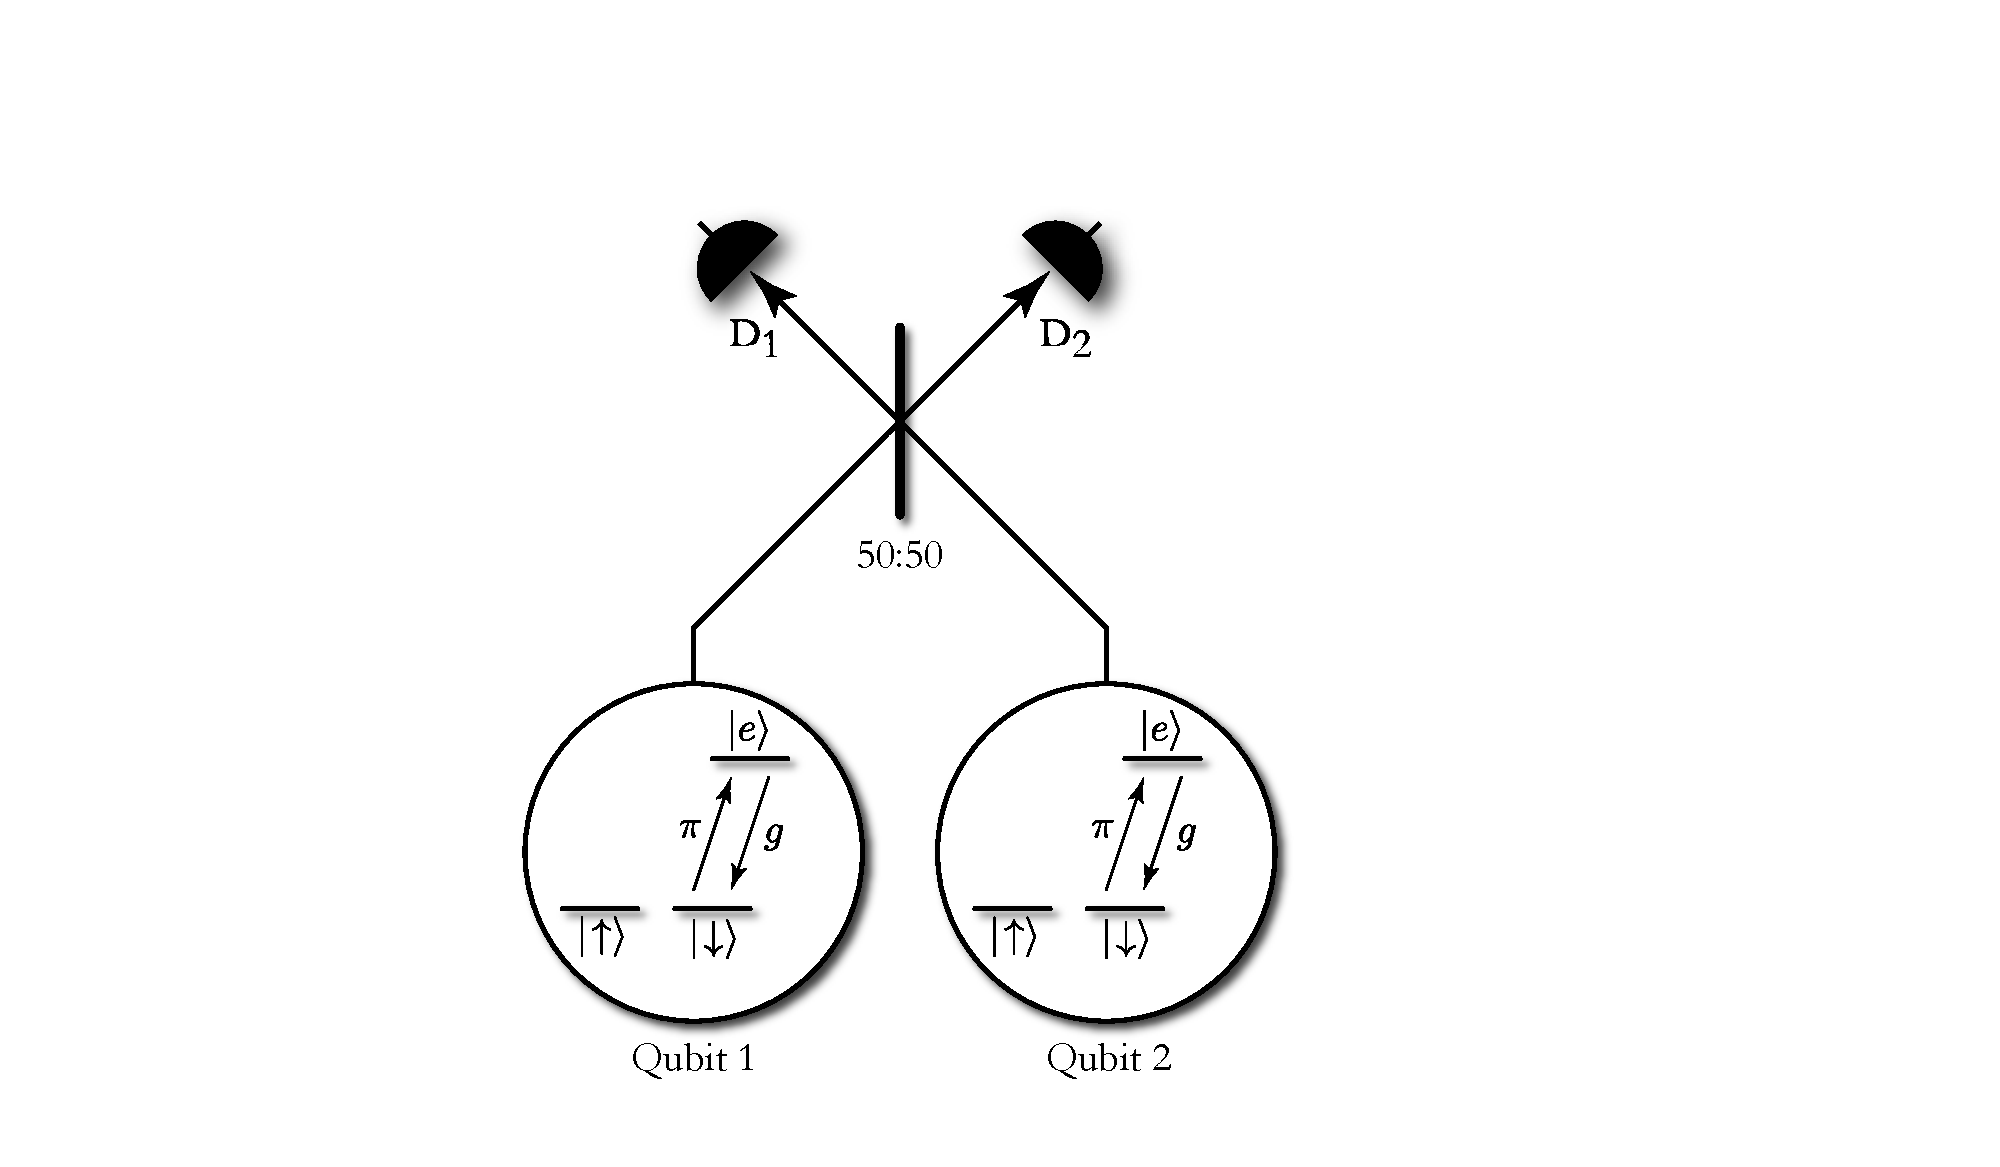
\includegraphics[width=0.75\columnwidth]{barrett_kok}
\caption{Two atomic systems in $\lambda$-configurations, each coupled with an optical mode. An entangling operation between them is mediated via linear optics which-path erasure. Each system contains two degenerate ground states, which jointly encode a qubit ($\ket{\!\uparrow}$, $\ket{\!\downarrow}$), and an additional excited state ($\ket{e}$), which only couples to the $\ket{\!\downarrow}$ state. A $\pi$-pulse excites the electron from the $\ket{\!\downarrow}$ to the $\ket{e}$ state, after which emission of a photon is associated with a coherent relaxation back to $\ket{\!\downarrow}$. If the two optical modes are interfered on a 50:50 beamsplitter, and a single photon is detected between the two photo-detectors, $D_1$ and $D_2$, the two emission processes become indistinguishable, and which-path erasure entangles the two qubits into a maximally entangled Bell-pair. More complicated networks based on this entangling operation allow the preparation of cluster states, enabling universal quantum computation. In a quantum networking context, the matter qubits could be held by a client, and the optical interferometry implementing the computation outsourced to the cloud, i.e the PBS, $D_1$ and $D_2$ are implemented in the cloud.} \label{fig:barrett_kok}
\end{figure}

The attractive feature of this type of approach is that the actual entanglement is generated using all-optical operations, despite the underlying logical qubits being stationary and potentially physically separated a long distance apart, mitigating the need for direct matter-matter interactions, and enabling distributed computation. Optical interfacing is discussed in Sec.~\ref{sec:opt_inter}. This allows the entangling operations to be performed remotely in the cloud, without physically moving the stationary qubits. Such hybrid systems present an interesting platform for cloud quantum computing -- despite the qubits being stationary, we are able to outsource the interactions between them to distant servers.

Importantly, the beamsplitter mediating the which-path erasure is based upon HOM interference, and therefore does not require interferometric stability, making the outsourcing process relatively robust.

Expanding upon this idea, we can envisage distributed models for quantum computation, where the qubits needn't even be of the same physical medium. We could, for example, entangle quantum dot qubits, atomic qubits, and atomic ensemble qubits with one another by coupling them to optical modes and performing which-path erasure between them. This enables distributed quantum computation between hosts possessing quantum infrastructure comprising different physical mediums (provided the photons emitted by those systems may be made indistinguishable, such that HOM interference is possible).

%
% Encrypted Quantum Computation
%

\subsection{Encrypted quantum computation} \label{sec:homo_blind}

Extremely important to many high-performance data-processing applications is security, as proprietary or sensitive data may be being dealt with. To address this, two models for outsourced quantum computation exist for addressing this -- \emph{homomorphic encryption} \cite{???, gentry2009fully, van2010fully} and \emph{blind quantum computation} \cite{???, bib:blind2, bib:blind3, bib:blind1, PhysRevLett.108.200502, bib:Morimae3486, bib:Morimae5460, bib:Morimae3966}.

In both cases, Alice has secret data, and wishes to not only ensure that an interceptor is unable to read it, but that the server performing the computation isn't able to either -- she trusts no one. That is, she wishes the data to be processed in encrypted form, without first requiring decryption.

The difference between the two protocols lies in the treatment of algorithms. In homomorphic encryption, Alice provides only the data, whereas Bob provides the processing and the algorithm it implements (which he would also like to keep to himself). In blind computing, Alice provides both the algorithm \emph{and} the data, and wishes \emph{both} to remain secret. Both of these protocols seem like very challenging goals, yet significant developments have been made on both fronts. Classical homomorphic encryption has only been described very recently \cite{bib:gentry2009fully, bib:van2010fully}. \comment{What is the overhead in classical resources. What about classical blind computation?}

In the usual circuit model, blind quantum computation has been shown to be viable, and optimal bounds derived. Similarly, such protocols have been described \cite{homoCS} in the cluster state model (Sec.~\ref{sec:CSQC}). For universal computation, such protocols necessarily require classical interaction between the client and host. However, it was shown that in some restricted (i.e non-universal) models for optical quantum computation, specifically {\sc BosonSampling} and quantum walks, non-interactive homomorphic encryption may be implemented almost optimally.

These encryption protocols induce a resource overhead in circuit size and number of qubits involved in the computation, with efficient scaling. They deliver information-theoretically secure data-hiding, enabling trustworthy outsourced processing of encrypted data, independent of the attack.

%
% Passive Linear Optics
%

\subsubsection{Passive linear optics}

It was recently shown that processing photonic states using passive linear optics may be trivially homomorphically encrypted with the addition of additional photons and randomised polarisation rotations on the inputs \cite{bib:RohdeQWEnc12}. This encryption does not require any client/server interaction, remaining completely passive, yet achieving near optimal secrecy.

For $m$ modes, the resource requirements are:
\begin{itemize}
\item $m$ single-photons -- one per input mode.
\item $m$ classically controlled wave-plates, able to implement arbitrary polarisation rotations.
\item $m$ polarisation filters.
\item $m$ photo-detectors.
\end{itemize}
The full protocol is given in Alg.~\ref{tab:homo_LO}.

\begin{table}[!htb]
\fbox{\parbox{0.965\columnwidth}{\tt
function HomomorphicLinearOptics($S$):
\begin{enumerate}
    \item Alice meditates upon, but needn't actually prepare the state,
    \begin{align}
    \ket\psi_\mathrm{number} = \otimes_{i=1}^m \ket{S_i},    
    \end{align}
    where
    \begin{align}
S_i\in\{0,1\},
    \end{align}
is the photon-number of the $i$th mode.
   \item Alice prepares a polarisation-encoded input state by making the substitutions from the photon-number basis into the polarisation basis, 
   \begin{align}
   \ket{0}&\to\ket{H}, \nonumber \\
   \ket{1}&\to\ket{V},
   \end{align}
   to obtain $\ket\psi_\mathrm{pol}$, containing $m$ photons in total, one per mode.
   \item Alice chooses a random private key $k$ as a real number from the uniform distribution,
   \begin{align}
    k\in(0,2\pi).
    \end{align}
    \item Alice prepares the encoded state by applying the same polarisation rotation (using wave-plates), of angle $k$, to each mode,
   \begin{align}
   \ket\psi_\mathrm{enc} = \hat{R}(k)^{\otimes m}\ket\psi_\mathrm{pol},
   \end{align}
   where,
   \begin{align}
   \hat{R}(\theta) = \left(\begin{array}{cc}
\mathrm{cos}\,\theta & -\mathrm{sin}\,\theta \\
\mathrm{sin}\,\theta & \mathrm{cos}\,\theta \end{array}\right).
   \end{align}
    \item Alice sends $\ket\psi_\mathrm{enc}$ to Bob.
    \item Bob applies processing using his linear optics computer, to obtain,
    \begin{align}
    \ket\psi_\mathrm{enc\,comp} = \hat{U} \ket\psi_\mathrm{enc},
    \end{align}
    \item Bob returns $\ket\psi_\mathrm{enc\,comp}$ to Alice.
    \item Alice applies the inverse of the encoding operation,
    \begin{align}
    \ket\psi_\mathrm{comp} = \hat{R}(-k)^{\otimes m}\ket\psi_\mathrm{enc\,comp}.
    \end{align}
    \item Alice applies polarisation filters to $\ket\psi_\mathrm{comp}$, discarding horizontally polarised photons.
    \item The remaining vertically polarised state is Alice's unencrypted output of the computation.
    \item $\Box$
\end{enumerate}}}
\caption{Protocol for implementing homomorphic encryption on photonic, passive linear optics.} \label{tab:homo_LO}
\end{table}

The key idea here is that orthogonal polarisations do not interfere with one another under linear optics evolution. Thus, by inserting additional orthogonal `dummy' photons, and applying random polarisation rotations, we can confuse any eavesdropper as to which photons belong to the computation, thereby hiding the secret data from them.

Using this protocol, it was shown that the probability of Bob correctly guessing Alice's input string approaches\footnote{This is in the asymptotic limit where the key $k$ is chosen with infinite precision. In practise, one will have to suffice with some limited precision in the choice of $k$, since an infinite-precision real number is effectively an infinitely long private key. Practically, one could choose $k$ as some integer multiple of \mbox{$2\pi/d$}, where $d$ is the number of distinct keys. In this case, the information security of the protocol increases with $d$. This relationship is provided by \cite{bib:RohdeQWEnc12}.},
\begin{align}
P_\mathrm{guess} = \sqrt{\frac{8}{\pi m}},
\end{align}
for sufficiently large $m$, which asymptotically (but unfortunately only polynomially) approaches 0. Furthermore, because a single computation requires Alice to perform only a single call to Bob's algorithm, which we treat as a black box, Alice gains minimum knowledge about Bob's secret algorithm.

%
% Coherent State Computation
%

\subsubsection{Coherent state computation}

\comment{To do}

%
% Cluster States
%

\subsubsection{Cluster states}

\comment{To do}

Most simply, if Alice has the limited quantum resources required to perform single-qubit measurements, and she knows the algorithm she wishes to implement, then by outsourcing just the cluster state preparation stage, whilst performing the single-qubit measurements herself, she can obviously obtain \emph{perfect} secrecy of both her data and her algorithm.

Homomorphic and blind quantum computing have been described natively to the cluster state model \cite{homoCS}, and in fact are conceptually more straightforward to understand in this formalism. 

%
% Universal Quantum Computation
%

\subsubsection{Universal quantum computation}

\comment{To do}

%
% Modularised Quantum Computation
%

\subsection{Modularised quantum computation} \label{sec:module}

How does one build a large-scale quantum computer, given the extremely daunting technological requirements and high costs? In any industry, economies of scale allow the mass production, and rapid reduction in price of technology. To achieve this, we must find a way to make quantum technologies commodity items, which avoid all the hassle of customised cutting-edge labs. What we really desire is production-line `Lego for Adults{\texttrademark}', allowing ad hoc connection of \emph{modules}, which implement small subsections of a large computation \cite{bib:FowlerPrivate}.

We envisage that physically, a module is a black box with optical interconnects, that may be interconnected to form an arbitrary topology. The user remains oblivious to the inner workings of the modules. The modules could all be identical, just patched together differently, paving the way for their mass production, and an associated quantum equivalent of Moore's Law, allowing them to become off-the-shelf commodity items over time. Then the cost of a quantum computer would simply scale linearly with its number of qubits.

The modules forming a particular computation could either be all owned by a single well-resourced operator, or alternately might be shared across multiple hosts, who network them remotely using EO's between emitted photons.

In Sec.~\ref{sec:dist_QC} we introduced the notion of distributed quantum computation. There the motivation was to enable a computation to be distributed across multiple servers, which either parallelise computation or process it as a pipeline in series.

An alternate direction, for economic reasons, is that it is unviable for a single server to host an entire computation. Rather, hosts will have limited capability, and performing large-scale computations will require employing a potentially large number of hosts cooperating and sharing resources with one another\footnote{Even some present-day massive-scale data processing and storage protocols are implemented virtually across multiple large-scale data-centres, which, for example, automatically handle geographically decentralised data redundancy and processing. Google and Amazon, for example, provide cloud services for this purpose, employed both internally, and licensed out to third parties, and the Apache Cassandra project provides an open-source equivalent. The key is for the underlying protocol to abstract this away from the user, such that they interface with the data as though it were a local asset.}. This can be regarded as the most general incarnation of distributed computation.

This is not the same motivation as for in-series computation, where different servers in the pipeline have different proprietary algorithms as subroutines of a larger computation. And it also differs from in-parallel computation, where multiple servers implement the same algorithm on different data, which is subsequently merged by a root node, as per, for example, a {\sc MapReduce}-style protocol.

Instead, the motivation is one of economics. First, individual servers will have finite resources, but there may be many of them, which can be networked to implement a larger algorithm virtually. Second, because the modules in the architecture are identical and lend themselves to mass production, one can expect more favourable economics than that offered by a provider who sells full-fledged, customised quantum computers, which do not lend themselves to the same level of mass production.

The concept of this model is best explained using the optical cluster state formalism (Sec.~\ref{sec:CSQC}), which lends itself naturally to this approach. A rectangular lattice graph is sufficient for universal quantum computation, even if the cluster state graph is not local (but classical communication between nodes is allowed).

Let us first assume that we wish to construct a cluster state with $n_\mathrm{logical}$ logical qubits. We additionally allow each logical qubit to be the root node of a graph with a $+$-structure, where each branch comprises $n_\mathrm{ancilla}$ ancillary physical qubits. These are sometimes referred to as \emph{micro-clusters} \cite{bib:Nielsen04}. A single micro-cluster collectively forms a single \emph{module} in the topology. Our goal is to fuse modules via nearest neighbour entanglement to build up the desired distributed cluster state.

\begin{figure}[!htb]
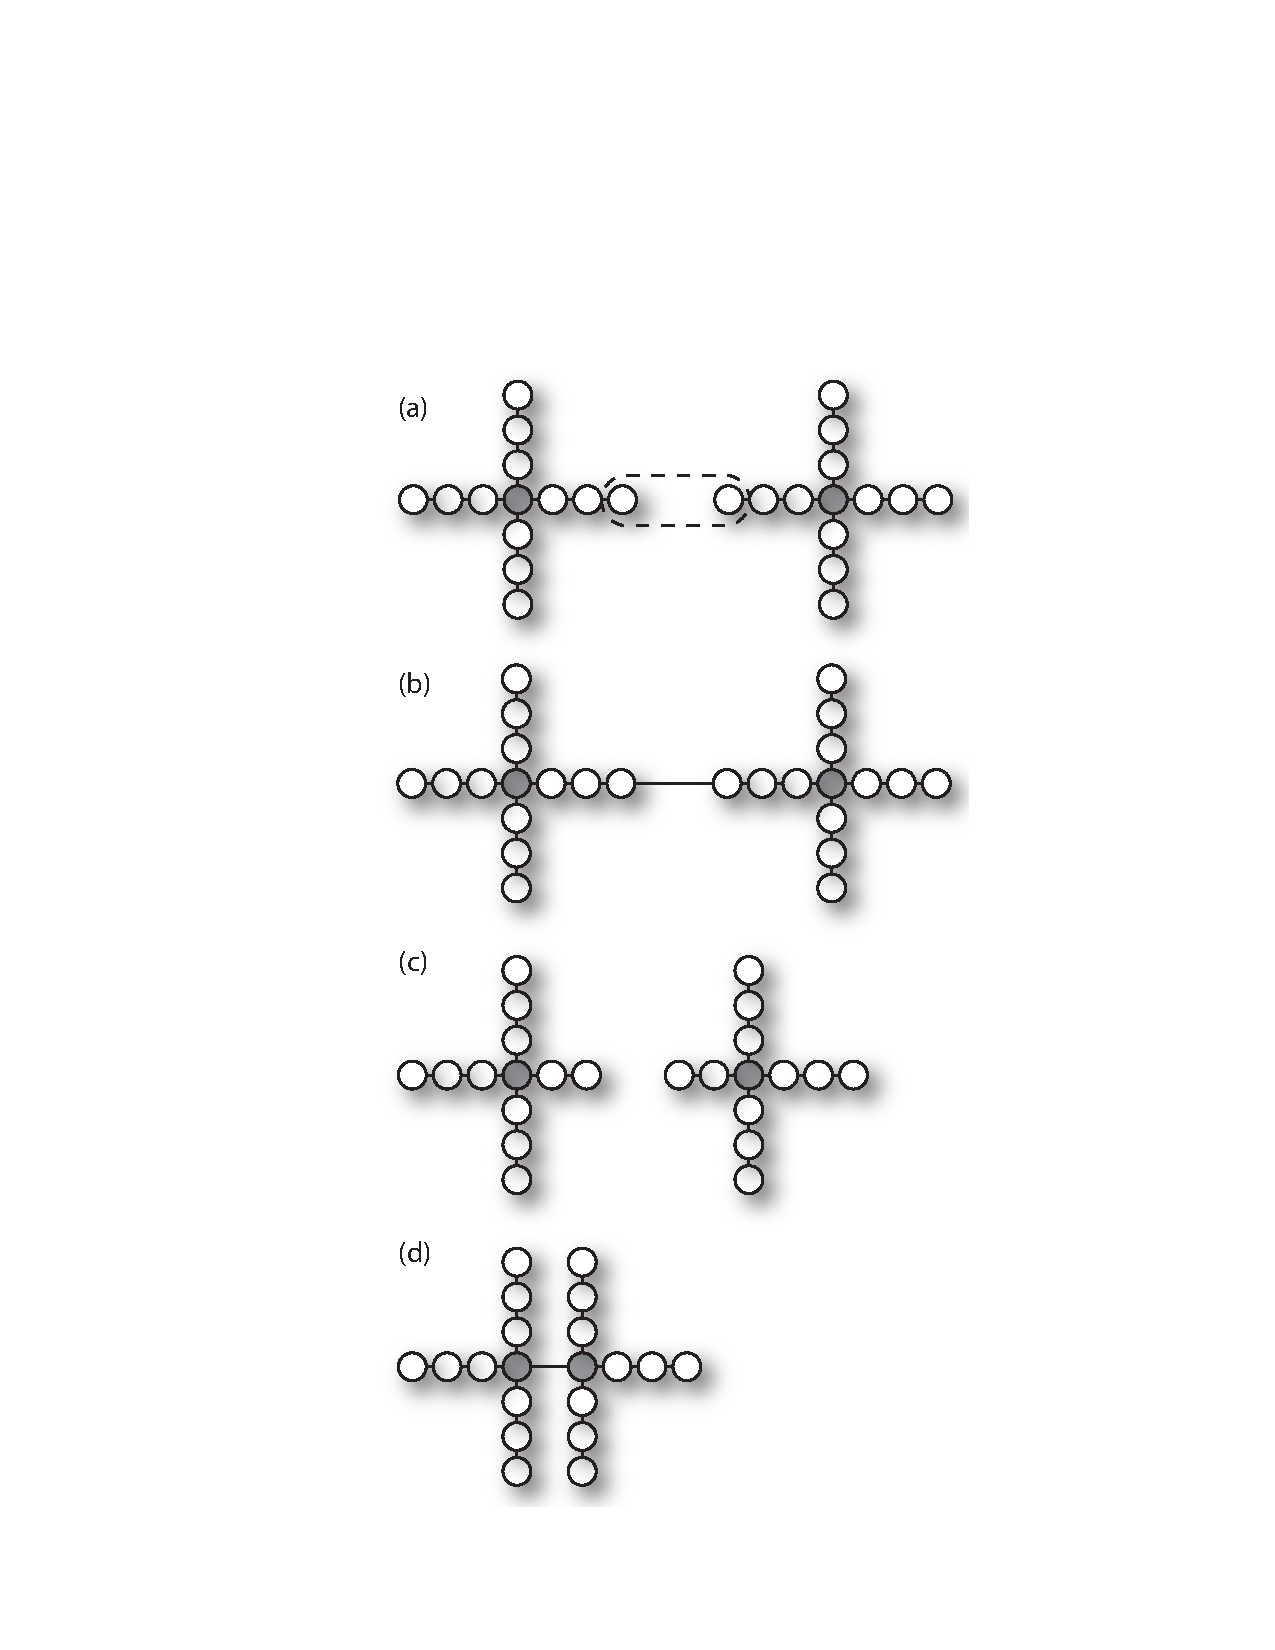
\includegraphics[width=0.9\columnwidth]{cluster_ident}
\caption{Several cluster state identities for modularised quantum computation. (a) Two cluster states with a $+$-topology are fused together using an EO (dashed). (b) Upon success, an edge is created between the respective qubits. (c) Upon failure, both qubits are effectively measured in the $\hat{Z}$ basis, thereby removing them, and any associated edges, from the graph. (d) Following a successful EO, the unwanted ancillary qubits may be eliminated using measurements in the $\hat{Y}$ basis, creating edges between their neighbours. If the grey qubits represent the desired logical qubits, this can be used to remove the remainder of the branches emanating from them.} \label{fig:plus_cluster_ident}
\end{figure}

We arrange the modules to internally represent a $+$-topology where each node has neighbouring branches in each of the up/down/left/right directions. But we imagine the situation whereby each logical qubit, along with its respective ancillary branches, is held by a different server. Thus, the final cluster state is truly decentralised across all the servers, and in general entire computations cannot be performed locally.

Using the ancillary states in the respective directions, we attempt to fuse neighbouring clusters using entangling operations (EO's), such as CZ gates (e.g a KLM CZ gate), linear optics \emph{fusion gates} (i.e rotated polarising beamsplitters followed by photo-detection) \cite{bib:BrowneRudolph05}, or atoms with a $\lambda$-configuration coupled to photons \cite{bib:BarrettKok05}, which undergo which-path erasure (Sec.~\ref{sec:hybrid}). Importantly, using the fusion gate and which-path erasure approaches, only a single beamsplitter is required to perform the EO, which only necessitates high-visibility HOM interference, mitigating the need for far more challenging interferometric (MZ) stability. This is delightful, as current leading quantum optics experiments routinely achieve HOM visibilities well in excess of 99\% \cite{???}.

When an EO is successful, we have fused two modules together, albeit potentially with some leftover ancillary states between the logical qubits. When it fails, we have lost the respective ancillary states, and we attempt again using the next ancillary qubits in each of the the respective branches -- a kind of {\sc `Repeat Until Success'} strategy. The bonding only fails if all $n_\mathrm{ancilla}$ EO's fail.

Note, however, that longer ancillary arms provide more opportunity for errors to accumulate \cite{bib:RohdeRalphMunro07}. Thus, despite its tolerance against gate failure, it is nonetheless highly desirable for EO's to be as deterministic as possible, so as to minimise the required number of ancillary qubits.

Upon successful bonding, any remaining ancillary qubits between the respective logical qubits are measured in the $\hat{Y}$ basis to remove them from the graph, whilst connecting their neighbours, leaving the two respective logical qubits as nearest neighbours in the graph. Now each module contains exactly one logical qubit, connected as desired to neighbouring modules. The relevant identities are shown in Fig.~\ref{fig:plus_cluster_ident}. Our goal is for the entire graph to have a lattice structure, once ancillary qubits have been measured out, as illustrated in Fig.~\ref{fig:module}.

\begin{figure}[!htb]
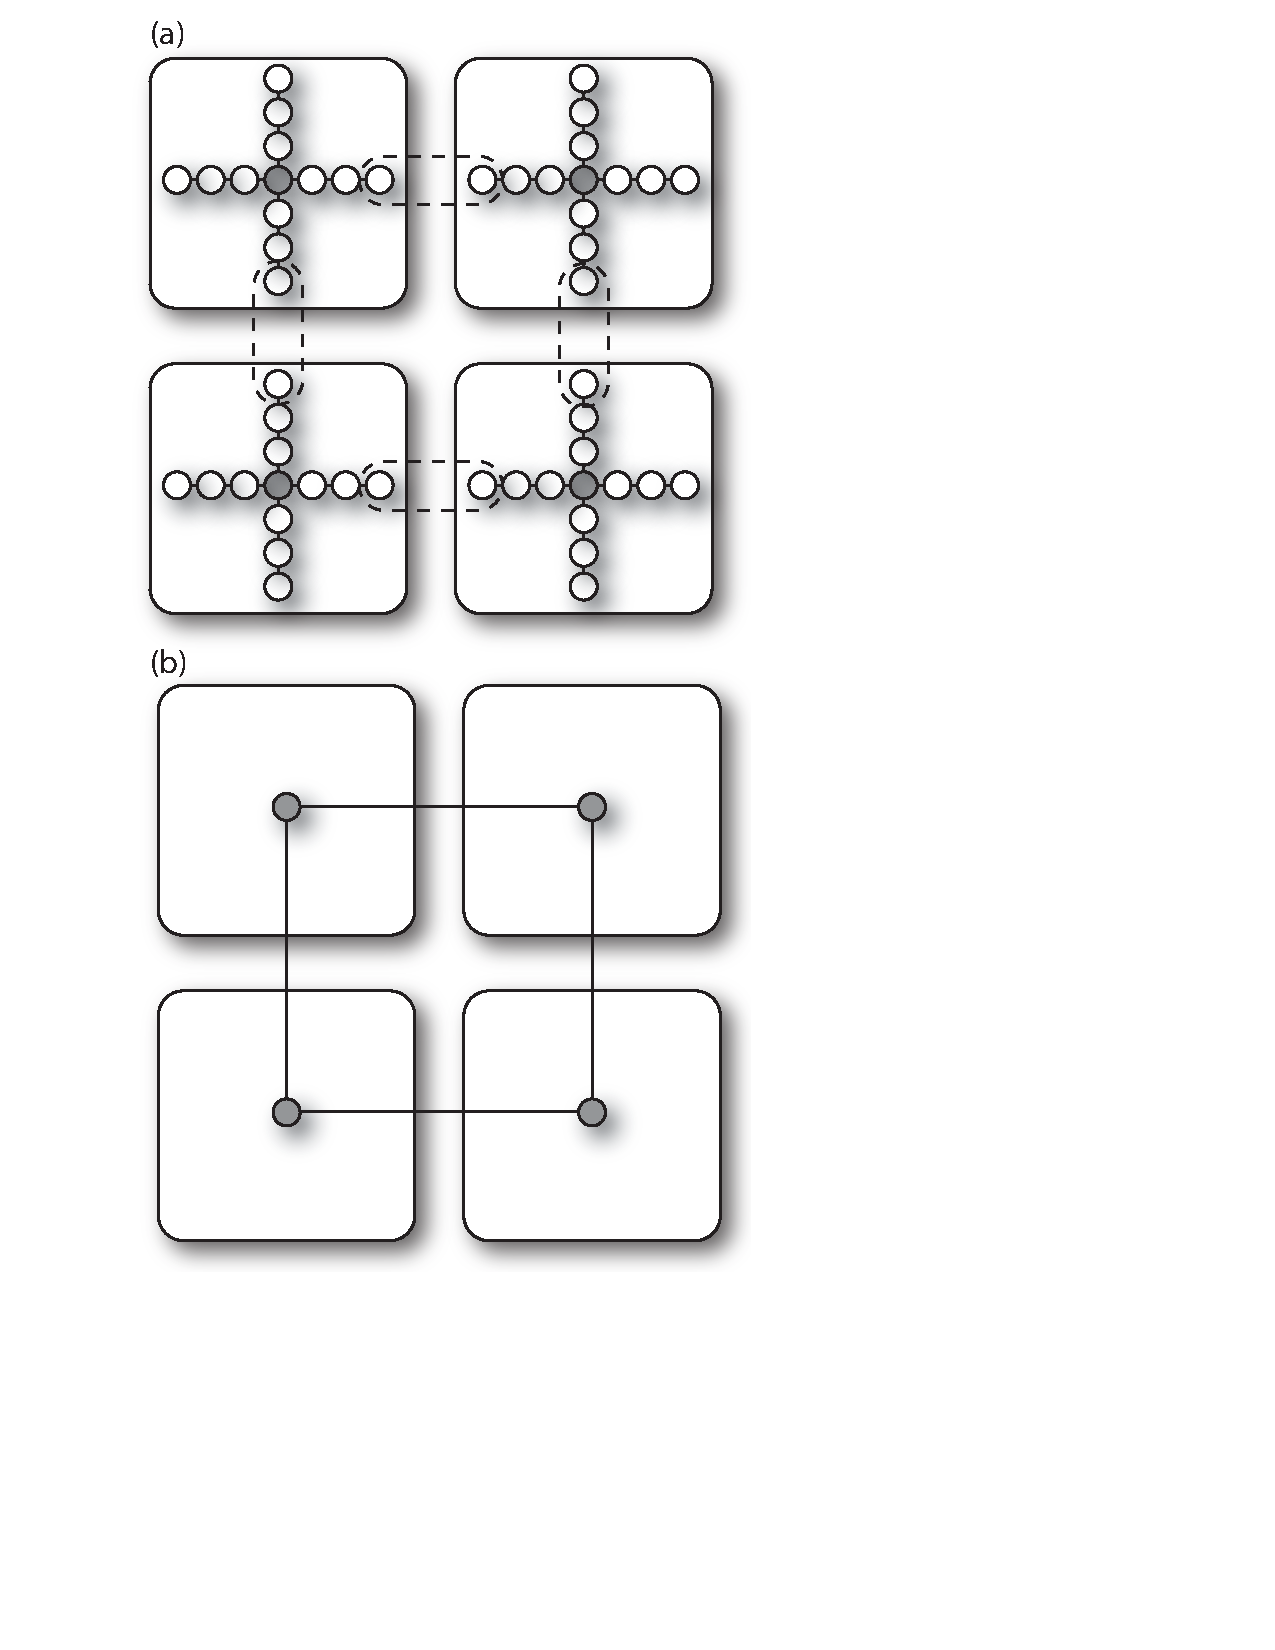
\includegraphics[width=0.8\columnwidth]{module}
\caption{The modularised approach to scalable and economically efficient, distributed quantum computation using cluster states. The modules are all identical, and can be arbitrarily patched to one another, allowing the construction of arbitrary graph topologies. Because the modules are all identical, one might hope that mass production and economy of scale will drive down the cost of modules. We consider a simple \mbox{$2\times 2$} case where each module (rounded rectangles) comprises a single logical qubit (centre of each module in grey) and a number of ancillary qubits (white in each module), which facilitate bonding the logical qubits of nearest neighbours. The preparation of the modules is performed via nearest neighbour EO's (dashed ellipses), beginning at the end of branches, and working towards the root node upon each failure, until (hopefully) an EO is successful. (a) A \mbox{$2\times 2$} lattice of modules with their respective ancillary qubits. We attempt to bond the endpoints of chains using EO's. (b) Upon measuring the remaining ancillary qubits in the $\hat{Y}$ basis, only the logical qubits remain, with nearest neighbour bonds between adjacent modules, creating a distributed cluster state.} \label{fig:module}
\end{figure}

This approach has been shown to be resource-efficient \cite{bib:YoranReznik03, bib:Nielsen04}. Let us perform a rudimentary analysis of the resource scaling of this type of approach. The probability of successfully creating an edge between two modules is,
\begin{align}
p_\mathrm{success} = 1 - {p_\mathrm{failure}}^{n_\mathrm{ancilla}},
\end{align}
where $p_\mathrm{success}$ is the probability of joining two modules, $p_\mathrm{failure}$ is the probability that a single EO fails, and $n_\mathrm{ancilla}$ is the number of ancillary qubits per chain. $p_\mathrm{success}$ can be made arbitrarily close to unity with sufficiently long ancillary chains, the required length of whom scales as,
\begin{align}
n_\mathrm{ancilla} = \frac{\mathrm{log}(1-p_\mathrm{success})}{\mathrm{log}(p_\mathrm{failure})}.
\end{align}

Now, for simplicity we will consider the preparation of linear cluster states, although these ideas can easily be extended to more complex topologies, such as 2D lattice graphs.

Let us assume we have a `primary' linear topology of modules, which we will incrementally attempt to `grow' by tacking on new modules to the end. When we do so, with probability $p_\mathrm{success}$ we grow the length of the primary by 1, otherwise we decrement it by 1. This proceeds as a random walk, with on average \mbox{$2p_\mathrm{success}-1$} new qubits added to the primary per time-step. Provided this number is positive, i.e \mbox{$p_\mathrm{success}>1/2$}, which can always be achieved with sufficient $n_\mathrm{ancilla}$, the length of the primary grows linearly over time, allowing efficient state preparation.

This is just a very primitive model for preparing linear cluster states, using an equally primitive {\sc Incremental} strategy for constructing them using non-deterministic gates. As discussed in Sec.~\ref{sec:CSQC}, much further work has been performed on the resource scaling of efficiently preparing cluster states of different graph topologies using different non-deterministic bonding strategies.

Of course, we have used the most simple model for modules, where each accommodates a single logical qubit. In due course, we would expect commodity modules to become far more capable, and resource scaling to improve. We might envisage that each module houses a small square lattice of logical qubits, as shown in Fig.~\ref{fig:larger_module}, and the interconnects between them glue them together like a patchwork quilt.

\begin{figure}[!htb]
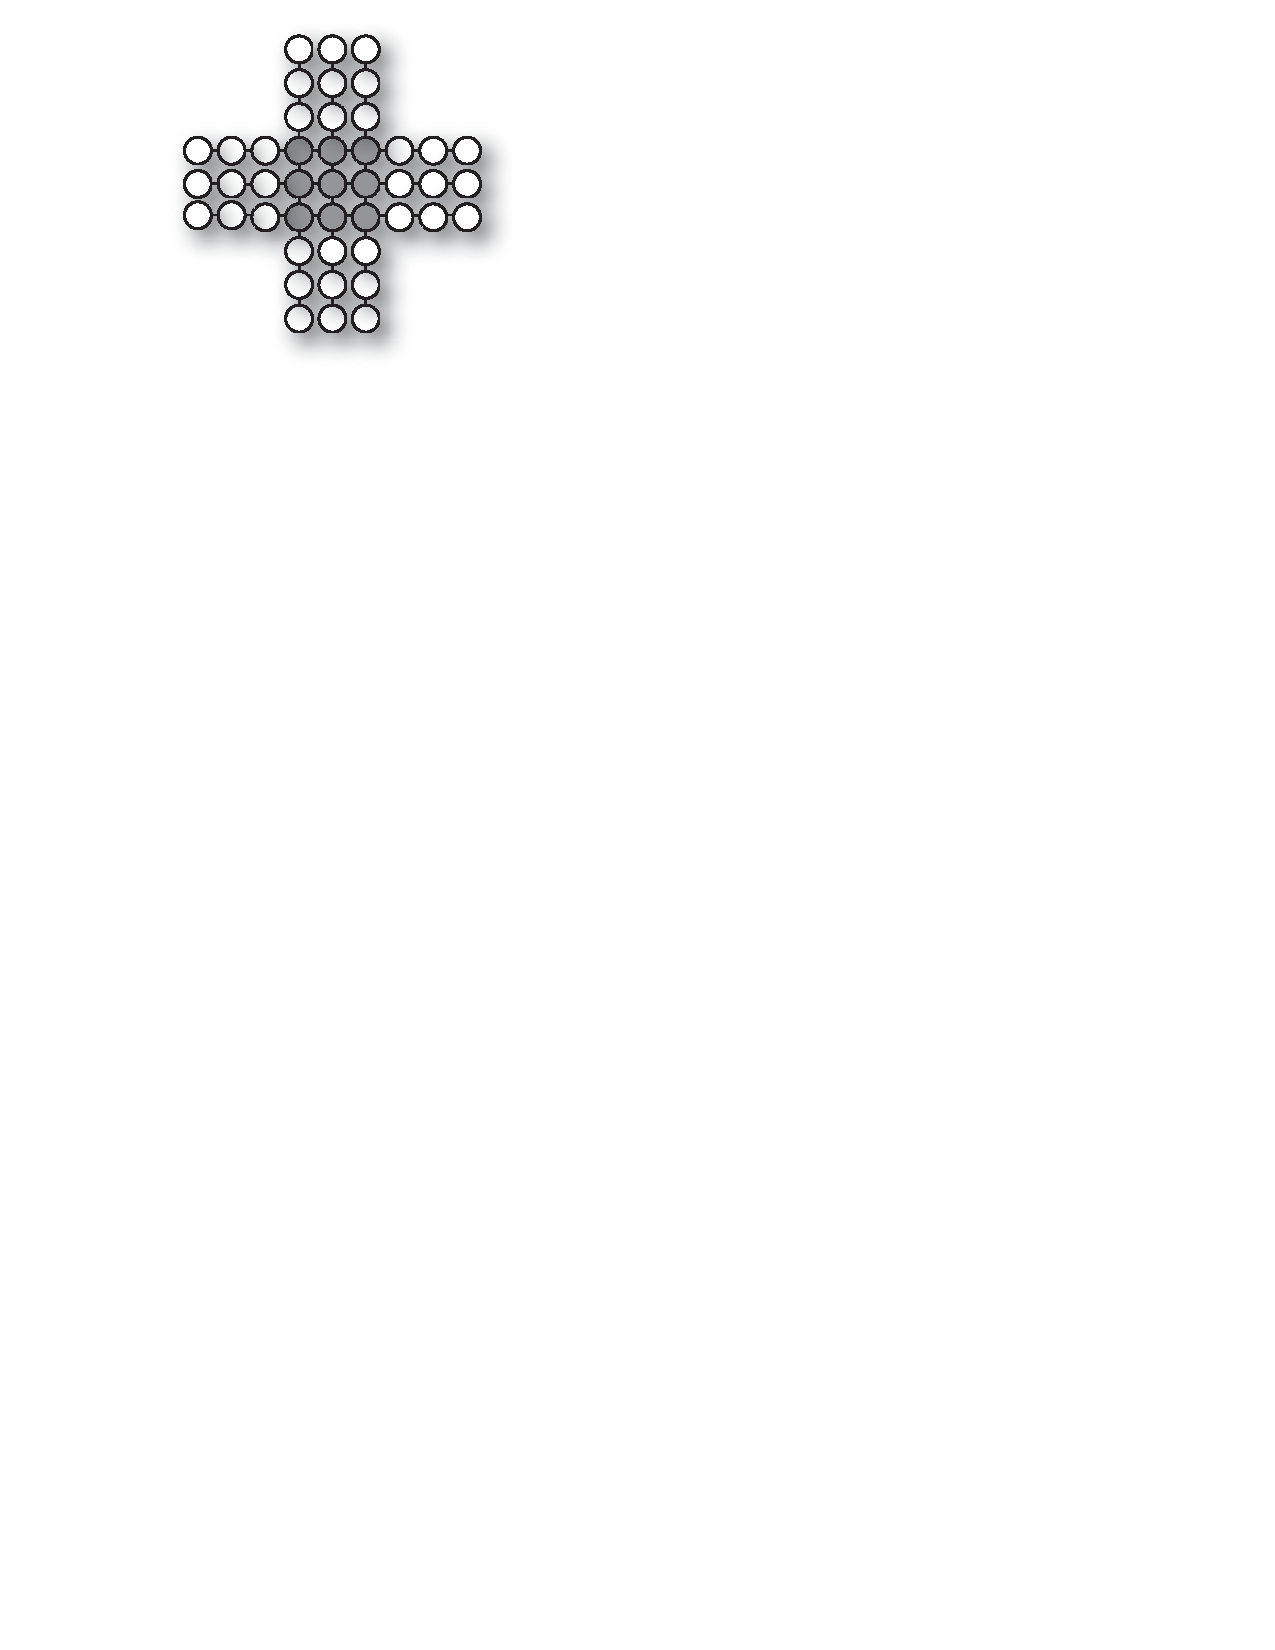
\includegraphics[width=0.6\columnwidth]{larger_module}
\caption{A larger cluster state module comprising a \mbox{$3\times 3$} lattice of logical qubits (grey), and dangling arms of ancillary qubits (white) in each direction for joining them to neighbouring modules. Fusing these modules enables the `patchwork' preparation of large, distributed lattices.} \label{fig:larger_module}
\end{figure}

%
% Entanglement - The Ultimate Quantum Resource
%

\section{Entanglement -- The ultimate quantum resource} \label{sec:ent_ultimate}

As we have seen, the diversity of quantum states that may be communicated, and quantum protocols that may be implemented over the quantum internet is extremely diverse, encompassing many different types of encodings and communications protocols.

Considering just the protocols that may be implemented over quantum networks discussed in detail in Sec.~\ref{sec:protocols_quant_int}, one might ask whether there is a single primitive resource that might be applicable to all, or at least most of these quantum protocols, thereby reducing the technological requirements of the quantum channels forming the network.

It turns out that there is one particularly useful quantum resource, that finds applicability in most of these protocols -- entanglement, specifically in the form of Bell-pairs (Sec.~\ref{sec:bell_state_res}).

In brief, Bell-pairs find applicability in, amongst many others, the following protocols:
\begin{itemize}
\item Cluster states (Sec.~\ref{sec:CSQC}): A Bell-pair is also a two-qubit cluster state, a supply of which can be employed in fusion strategies to prepare larger cluster states, enabling measurement based quantum computation.
\item Quantum teleportation (Sec.~\ref{sec:teleport}): A shared Bell-pair between Alice and Bob forms the elementary quantum resource upon which the teleportation protocol is constructed.
\item QKD (Sec.~\ref{sec:QKD}): The E91 protocol in built upon a reliable stream of distributed Bell-pairs.
\item Modularised quantum computation (Sec.~\ref{sec:module}): Using Bell-pairs, entanglement swapping (Sec.~\ref{sec:swapping}) can be employed to fuse neighbouring modules together using operations local to each module.
\end{itemize}

Thus, we see that Bell-pairs form a ubiquitous resource, covering the most significant quantum protocols -- quantum computation, distributed quantum computation, and quantum cryptography. This warrants special treatment of entanglement distribution, as a fundamental building block for the quantum internet.

One might envisage a quantum internet in which a central server, who specialises in Bell state preparation, serves the sole role of pumping out Bell-pairs across the internet to whoever requests them, who subsequently use them for protocols such as those mentioned above. This could be in the form of a server transmitting over fibre networks, or a satellite in orbit, transmitting at an intercontinental level.

What's the advantage of this approach to quantum networking? There are several:
\begin{itemize}
\item Dedicated servers can specialise in this one particular task, as can be the transmission infrastructure. The server needn't concern itself with the nitty-gritty of the protocols implemented by the end user.
\item Unlike generic quantum states, Bell-pairs are known states that can be infinitely reproduced, without having to worry about no-cloning limitations.
\item Photonic Bell-pairs are easily prepared via SPDC at very high repetition rates (\mbox{$\sim 100$MHz}), enabling rapid state preparation.
\item Importantly, QoS is a lesser issue in most scenarios. We can employ a {\sc Send and Forget} protocol for the distribution of entanglement (much like classical UDP). Since every Bell-pair is identical, we needn't be concerned about missing ones, and there are no constraints imposed by the no-cloning theorem. Instead we can simply wait for the next one, knowing it will be exactly the same. We call this the {\sc Shotgun} approach -- keep firing away until we hit something.
\end{itemize}

In addition to entanglement distribution, entangling measurements, e.g Bell state projections (Sec.~\ref{sec:bell_proj}), may be used as a primitive for many protocols. This is effectively entangled state distribution in reverse, whereby two clients transmit states to a host, who performs a joint entangling measurement upon them. For example, in the modularised model for cluster state quantum computing (Sec.~\ref{sec:module}), two adjacent modules might transmit optical qubits to a satellite, which projects them into the Bell basis, thereby creating a link between the respective modules, potentially far apart. This isn't as powerful as entangled state distribution, since it cannot be used for, for example, E91 QKD, but nonetheless remains a powerful primitive for many protocols.

These observations lead us to naturally conclude that a quantum network specialised to this one particular task -- entanglement distribution or entangling measurements -- would already be immensely useful, and on its own enable many key quantum protocols, such as the ones presented here in Sec.~\ref{sec:protocols_quant_int}.

%
% Quantum Repeater Networks
%

\subsection{Quantum repeater networks}

\cite{bib:DurBriegel999}

%
% State of the Art
%

\section{State of the art} \label{sec:state_of_the_art}

\comment{PROOF READ THIS SECTION AND CORRECT!}

When will we have the quantum internet? This is a question with as many answers as there are people one asks. And the developments of the different components of such an internet will be staggered and under continual development -- a quantum internet with the capacity for long-distance QKD will likely arrive far sooner than one supporting fully distributed, blind quantum computation.

In this section we discuss recent developments in and the state of the art of some of the most important quantum technologies and protocols, with a view to understand trends in the development of the field, so as to gauge the rate of progress. With this we aim to shed light on what quantum networking services could be readily implemented today, using present-day technology, and what is likely to be viable in the near future. %We then venture into the world of the unknown, and discuss how far technology must develop in order to enable the basic building blocks for a scalable quantum internet, implementing protocols of practical use.

We will very succinctly summarise a brief history of major recent developments in the field, without much elaboration. Rather our goal here is simply to very tersely summarise recent progress and the state of the art. The reader disinterested in a history lesson might skip this section.

%
% Quantum Teleportation & Entanglement Distribution
%

\subsection{Quantum teleportation \& entanglement distribution}

Quantum state teleportation (Sec.~\ref{sec:teleport}) is useful in its own right, as a means by which to transmit quantum states, but also as a primitive in larger protocols, such as the gate teleportation (Sec.~\ref{sec:teleport_gate}) employed by LOQC (Sec.~\ref{sec:KLM_univ}).

Since it was first proposed in 1993 \cite{bib:PRL_70_1895}, quantum state teleportation has attracted broad interest and been subject to widespread experimental demonstration across many physical architectures, becoming one of the most important protocols in quantum information science.

Single-qubit teleportation requires a single Bell-pair as a resource, after which an entangling measurement, followed by classical communication of the measurement outcome, completes the protocol.

For the generation of quantum entanglement, a significant breakthrough was made in 1995 by \cite{kwiat1995new}, who demonstrated a technique for the generation of high-intensity polarisation-entangled photon pairs. For the partial Bell state projection of two polarisation-encoded qubits, a 50:50 beamsplitter \cite{bib:Euro_25_559} was employed (Sec.~\ref{sec:bell_proj}).

The first experimental demonstration of photonic quantum teleportation was achieved in 1997 \cite{bib:Boumeester97}. Two photon-pairs were prepared by double-pumping a single nonlinear beta-barium borate (BBO) crystal: one pair employed as the entanglement source; the other to prepare the state to teleport via heralding. The partial Bell state measurement was implemented using which-path erasure at a beamsplitter, with an efficiency of 25\%. 

Since then, great effort has been invested into experimentally demonstrating quantum teleportation with not only photons, but also many other quantum systems.

One major experimental achievement for optical quantum state teleportation has been in the lengthening of the transmission distances -- either in fibre or free-space. In the pioneering work of \cite{bib:Nat_421_509}, they experimentally demonstrated quantum state teleportation between two labs, separated by 55m, but connected by a 2km long length of fiber, with photons at telecommunication wavelengths. The ability to implement this protocol over kilometre length-scales and at telecom wavelengths, arouses the exciting prospect that future quantum networks might be able to piggyback off existing telecom infrastructure, which would be a boon to the quantum industry.

In \cite{bib:Nat_430_849}, quantum teleportation over a distance of 600m across the River Danube in Vienna was implemented over fibre. Due to the relatively low photon detection efficiencies at telecom wavelengths, quantum teleportation over long-distance optical fibre became challenging. 

In 2008, quantum state teleportation was demonstrated between photonic and atomic qubits \cite{bib:Chen08}, a first step towards hybrid architectures (Sec.~\ref{sec:hybrid}).

In 2010, \cite{bib:Nat_Phot_4_376} demonstrated quantum teleportation over a 16km long, noisy, free-space channel between distant ground stations. This distance is of especial interest as it is significantly longer than the effective thickness of the atmosphere, equivalent to 5-10km of ground atmosphere \cite{bib:PRL_94_150501}. This is an exciting benchmark as it suggests that free-space ground-to-satellite teleportation may be viable.

Two years later in 2012, the teleportation distance in free-space was extended to 97km over Qinghai Lake \cite{bib:Nat_488_185}, and 143km between the two Canary Islands of La Palma and Tenerife \cite{bib:Nat_489_269}. These two works overcame the daunting challenges associated with source targeting and tracking, for long-distance, free-space quantum teleportation, and paved the way for future satellite-based quantum teleportation.

Accompanying the breakthrough of superconducting single-photon detectors with near-unit efficiency, 3-fold photo-detection for quantum teleportation was greatly enhanced by more than two orders of magnitude at telecom wavelengths, and the teleportation distance in optical fibre lengthened to 100km in 2015 \cite{bib:Optica_2_832}. Very recently, \cite{bib:Nat_Phot_10_671, bib:Nat_Phot_10_676} demonstrated quantum teleportation over fibre networks in Hefei and Calgary respectively, with lengths of dozens of kilometres. 

Another breakthrough achievement towards future long-distance quantum teleportation was the first quantum satellite for entanglement distribution, launched in August 2016 in China. In addition to teleportation, such a satellite-based entanglement source could facilitate intercontinental QKD. The responsible team is aiming to achieve quantum teleportation between ground stations and satellite, and even between pairs of distant ground stations, separated by over 1000km, using shared entanglement provided by the satellite \cite{bib:Nat_535_478}.

With the development of numerous quantum control technologies, more and more complex experimental demonstrations of quantum teleportation have been performed. In 2005, using 5-photon entanglement, open-destination teleportation was implemented \cite{bib:Nat_430_54}, whereby an unknown quantum state was teleported onto a superposition of 4 destination photons, and could be read out at any location -- a type of `broadcasting�.

In 2006, \cite{bib:Nat_Phys_2_678} successfully teleported the state of a two-photon composite system -- a breakthrough in the teleportation of a single particle onto a complex system comprising multiple particles. And in 2015, \cite{bib:Nat_518_516} demonstrated quantum teleportation over multiple degrees of freedom of a single optical mode.

Besides the widely used qubits encoded by discrete variables, the CV's of optical modes could also be utilised to encode quantum states for teleportation. The first experimental demonstration of this type was carried out in 1998 \cite{bib:Science_282_706}. The advantage of this teleportation protocol was that it could be deterministic in principle, thereby overcoming the obstacle of non-determinism inherent to partial Bell state projections using a PBS (Sec.~\ref{sec:bell_proj}).

15 years later in 2013, \cite{bib:Nat_500_315} exploited this advantage with a hybrid technique, and demonstrated the deterministic teleportation of photonic qubits.

In addition to linear optical systems, quantum teleportation has also attracted great interest in other physical architectures. Numerous demonstrations of quantum teleportation have been carried out in various systems, including atoms \cite{bib:Nat_Phys_9_400}, ions \cite{bib:Nat_429_734, bib:Nat_429_737}, electrons \cite{bib:Science_345_532}, and superconducting circuits \cite{bib:Nat_500_319}.

Hybrid schemes combining different physical systems have also been successfully demonstrated, such as teleportation between light and matter systems \cite{bib:Nat_443_557, bib:Nat_Comm_4_2744}. These hybrid technologies are expected to play an important role in future quantum networks, where the underlying physical architecture for (say) a quantum computation is non-optical, but optics mediates the communication of quantum information (Sec.~\ref{sec:hybrid}).

%
% Entanglement Swapping & Quantum Repeaters
%

\subsection{Entanglement swapping \& quantum repeaters}

Closely related to entanglement distribution is entanglement swapping (Sec.~\ref{sec:swapping}), where the goal is to entangle two remote parties, each of whom have one half of two distinct Bell-pairs. As discussed in Sec.~\ref{sec:ent_ultimate}, entanglement swapping will be of fundamental importance in networks treating entanglement distribution as the most fundamental elementary resource, making it of great importance to quantum networking, allowing the distribution of entanglement between distant parties, who are unable to communicate directly (i.e the entanglement distribution is `mediated').

The first experimental demonstration of entanglement swapping was presented in 1998 \cite{bib:PRL_80_3891}. By pumping a BBO crystal in a double-pass configuration, two pairs of polarisation-entangled photons were generated to demonstrate the scheme. A visibility of \mbox{$0.65$} was observed, which clearly surpasses the classical limit of \mbox{$0.5$}. This was later improved in 2001 to a visibility of \mbox{$0.84$} \cite{bib:PRL_86_4435}, which violates the Bell inequality (for which the threshold is $0.71$). 

Aside from `event-ready' mode, \cite{bib:JMO_47_2} proposed a delayed-choice mode of operation for entanglement swapping in 2000, where entanglement is produced a posteriori, after the entangled particles have been measured and may no longer even exist.

In 2001, \cite{bib:PRL_88_017903} designed and realised delayed-choice entanglement swapping. This was performed by adding two 10m optical fibre delays of about 50ns for both outputs of the Bell state measurement. Subsequently, in 2002 \cite{bib:PRA_66_024309} realised a delayed-choice entanglement swapping experiment with vacuum and one-photon quantum states. However, none of these demonstrations were active, random or delayed choice, which are required to ensure that photons cannot know in advance the basis choices for future measurements.

In 2012, \cite{bib:Nat_Phys_8_479} demonstrated an entanglement swapping experiment with active delayed choice. In their experiment, they designed a special interferometer to realise active switching between Bell state measurement and separation state measurement, and experimentally verified the entanglement-separability duality of the two photons. 

Subsequently, experimental demonstrations of entanglement swapping have evolved to become more complex and rigorous, finding uses in more sophisticated networking protocols.

In 2008, \cite{bib:PRL_101_080403} used three pairs of polarisation-entangled photons, and conducted two Bell state measurements to realise multistage entanglement swapping. \cite{bib:PRL_103_020501} demonstrated multi-particle entanglement swapping using a three-photon GHZ state. In 2013, \cite{bib:PRL_110_210403} demonstrated entanglement swapping between photons that never coexisted. In their experiment, entangled photons are not only separated spatially, but also temporally. In 2015, \cite{bib:PRL_114_100501} experimentally realised hybrid entanglement swapping between discrete- and CV optical systems.

To develop a practical quantum network, entanglement swapping between independent entangled photon sources is an important technique. In the past two decades, entanglement swapping has been demonstrated in a large number of experiments across many physical architectures. However, in most experiments, entangled photons are generated by using the same laser, and therefore do not meet the requirements for independence. Entanglement swapping based on independent entangled photon sources has been experimentally verified \cite{bib:PRL_96_110501, bib:Nat_Phys_3_692, bib:PRA_79_040302}, but the distinguishability caused by photon propagation in the channel is still a great obstacle to realising entanglement swapping using independent sources under realistic conditions.

In 2015, \cite{bib:Nat_526_682} for the first time achieved entanglement swapping using independent entangled photon sources separated by 1.3km in a real-world environment. However, the wavelength of the photons used in this experiment was 637nm (transmission loss \mbox{$\sim 15$dB/km}), which is not conducive to achieving long-distance entanglement swapping since it is far greater than the transmission loss of communication-band photons in fibre (\mbox{$\sim 0.2$dB/km}). Based on the techniques in \cite{bib:Nat_phot_10_671, bib:Nat_phot_10_676}, longer-distance entanglement swapping may be possible in the near future.

Entanglement swapping can also be directly used for QKD. Alice and Bob each have an entangled photon source, and one photon of each EPR pair is sent to a third-party measurement node, Eve. Similar to measurement-device-independent (MDI) QKD, the security of the generated private key does not depend on Eve's faithful execution of the operation. That is, Eve can be an untrusted third party. This MDI property also reflects the physical beauty of quantum teleportation. Bell state measurements do not reveal any information about the quantum state, but can be used to restore the transmitted quantum state. On the other hand, quantum entanglement occurs between the remaining photons in the EPR pair of Alice and Bob. \cite{bib:PRL_90_057902, bib:NJP_10_2008} suggest that an entangled photon source can be considered as a basis-independent light source for QKD. Thus, the QKD realised by entanglement swapping has the characteristics of MDI and light source independence.

An important application for entanglement swapping is that we can entangle spatially separated and independent matter qubits by coupling them with photons, upon which entanglement swapping is subsequently applied. This is an extremely important technique for hybrid quantum networks (Sec.~\ref{sec:hybrid}), where optical interactions mediate entanglement swapping between non-optical qubits.

Starting with two entangled atom-photon pairs, we can project the two atomic qubits into a maximally entangled state by performing a Bell state measurement on the two photons \cite{bib:Nature_428_153, bib:PRL_96_030404}. In 2007, \cite{bib:Nature_449_68} entangled two trapped atomic ions separated 1m apart using entanglement swapping, exploiting interference between photons emitted by the ions. The fidelity of the states of the entangled ions was $0.63(3)$. In subsequent experiments \cite{bib:PRL_100_150404}, the ion-ion entanglement fidelity was improved to $0.81$. Similarly, \cite{bib:Nature_454_1098} entangled two atomic ensembles, each originally with a single emitted photon, by performing a joint Bell state measurement on the two single photons after they had passed through a 300m fibre-based communication channel. In 2015, \cite{bib:Nature_526_682} generated robust entanglement (estimated state fidelity of $0.92\pm0.03$) between the two distant spins by entanglement swapping in the scheme of \cite{bib:PRA_71_060310, bib:Nature_497_86}. Such a high fidelity is sufficient to successfully perform loophole-free Bell inequality tests.

Entanglement swapping is a core element of quantum repeaters, which is of great significance to realising long-distance quantum communication. At present, the maximum transmission distance that can be achieved by QKD is 400km \cite{bib:arxiv_1606.06821}. Therefore, the communication distance is still a bottleneck restricting the development of quantum communication. Quantum repeaters, proposed in 1998 \cite{bib:PRL_81_5932}, combine entanglement swapping and quantum memory, which provides a potential solution to this problem.

The first proposed practical quantum repeater architecture was proposed in 2001 by Duan, Lukin, Cirac \& Zoller (DLCZ) \cite{bib:DLCZ}, using atomic ensembles and linear optics. To increase the repeater count-rate, various protocols \cite{bib:RMP_83_33, bib:PRA_79_042340, bib:PRA_92_012307, bib:PRA_81_052311, bib:PRA_81_052329, bib:NP_6_777, bib:PRL_112_250501} have been proposed.

In 2015, \cite{ncomms7787} introduced the concept of all-photonic quantum repeaters, based on flying qubits, which entirely mitigate the need for a matter quantum memory. 

Experimental demonstration of elementary segments of quantum repeaters were achieved by \cite{bib:Sc_316_1316, bib:Nat_454_1098}.

In order to develop practical quantum repeaters, there are many experimental techniques that must be developed, such as the multiplexing technique \cite{bib:PRA_76_050301, bib:PRA_82_010304, bib:PRL_113_053603, bib:PRL_98_060502} for constructing multimode memories. Techniques based on non-degenerate photon-pair sources \cite{bib:Nat_469_508, bib:Nat_469_512, bib:PRL_112_040504, bib:PRA_92_012329} and quantum frequency conversion \cite{bib:NP_6_894, bib:NC_5_3376} are being developed to obtain quantum memories compatible with photons at telecom wavelengths.

Aside from photonic systems, techniques based on other physical systems have also been developed \cite{bib:NP_11_37, bib:Sc_337_72, bib:N_484_195, bib:N_497_86}. In general, to enable scaling up to repeaters with several links, many techniques need to be considerably improved and simplified, and it appears there is still a long way to go before building a first practical, long-distance quantum repeater.

%
% Quantum Key Distribution
%

\subsection{Quantum key distribution}

With the development of quantum technology, QKD will gradually become more and more practical and economically accessible. Bennett, one of the proposers of the BB84 protocol, firstly demonstrated the protocol on an optical platform with a distance of 30cm \cite{bib:JC_5_3}. Since then, experiments have developed rapidly from indoor to outdoors, and from short distance to long distance, with commercial QKD units even available as off-the-shelf products.

In 1993, \cite{bib:EL_23_383} experimentally demonstrated quantum cryptography using polarised photons in optical fibre over more than 1km. \cite{bib:EL_29_634} operated a QKD experiment over 10km using phase-encoding. In 1995, \cite{bib:Arx0203118} realised an outdoor experiment over 67km using a plug-and-play system to automatically maintain stabilisation.

In 2007, \cite{bib:PRL_98_010505}, Los Alamos Nation Laboratory (LANL), \cite{bib:PRL_09_010503x} and \cite{bib:PRL_98_010504} demonstrated QKD experiments based on decoy-states over more than 100km almost simultaneously, marking the beginning of long-distance QKD.

In 2010, \cite{bib:OptExp_18_8587} reported an implementation of decoy-state QKD over a 200km optical fibre cable through photon polarisation with a final key rate of 15Hz.

In 2007, \cite{bib:NP_1_343} firstly realised a differential phase-shift (DPS) QKD protocol over a 42.1dB lossy channel and 200km of optical dispersion-shifted fibre.

In 2012, \cite{bib:OL_37_1008} realised the DPS protocol over 50dB channel loss and 260km of optical fibre using superconductive detectors, this is the first implementation of QKD over more than 50dB channel loss.

In 2009, \cite{bib:NJP_11_075003} realised the coherent one way (COW) protocol QKD system with a maximum range of 250km at 42.6dB channel loss using ultra-low-loss fibre, with secret bit rates up to 15Hz.
 
Apart from using the QKD scheme based on state preparation and measurement, schemes based on entanglement distribution, mainly the E91 \cite{bib:PRL_67_661} and BBM92 \cite{bib:PRL_68_557} protocols, have been demonstrated, which also undergoing extensive experimental investigation.

In 2005, \cite{bib:OE_13_202} distributed entanglement and single photons through over a free-space quantum channel, demonstrating the viability of free-space quantum communication. 

In 2006, \cite{bib:APL_89_101122} reported a complete experimental implementation of a QKD protocol over a free-space link using polarisation-entangled photon pairs.

In 2007, \cite{bib:NP_3_481} realised the BBM92 protocol QKD based on polarisation encoding over 144km.

The experiments listed above indicated that QKD protocols based on free-space entanglement distribution have the advantage of being less affected by decoherence, which lay a solid foundation for global and satellite-to-ground quantum communication. 

Fibre loss increases exponentially with distance. However, the loss of free-space transmission increases very little with distance,  mainly related to the thickness of the atmosphere. Therefore, it is a perfectly reasonable solution to construct the global quantum internet based on satellite communication. To verify the feasibility of a quantum channel between space and Earth, a European Union group successfully received weak light pulses emitted from a ground station and reflected by a mirror placed on a low-orbiting satellite with orbital altitude of 1485km in 2008 \cite{bib:NJP_10_033038}. In the context of rapidly moving platforms, \cite{bib:NP_7_382} realised QKD over 20km from an airplane to the ground in 2013. In the same year, \cite{bib:NP_7_387} successfully accomplished quantum communication with a hot-air balloon floating platform. The experiments on aeroplanes and hot-air balloon systems demonstrate the feasibility of quantum communication in the condition of rapid motion, vibration, and random movement of satellites. At present, many countries including America, Canada, the European Union, China and Japan pay great attention to and support for accelerating the development of satellite-to-ground quantum communication. The first quantum satellite was launched in August 2016 in China, and will open a platform for satellite-to-ground quantum communication at an intercontinental level \cite{bib:N_535_478}.

In addition to the ongoing expansion in distance, QKD is also being developed for point-to-point communication with quantum networks, which may be multi-user and of various and diverse topological structures. There is much competition and cooperation in this area. The network of the American Defence Advanced Research Projects Agency (DARPA) connected the three nodes -- Harvard University, Boston University, and the BBN company -- in 2005, later increasing this to 10 nodes \cite{bib:QCC_2006_83}.

Since 2006, the EU has established a `SECOQ' network, combining the efforts of 41 research and industrial organisations from 12 countries, including the UK, France, Germany, and Austria.

A typical network employing a trusted repeater paradigm, with 6 nodes and 8 links was demonstrated in Vienna in 2008 \cite{bib:NJP_11_075001}. In 2010, the National Institute of Communication Technology, together with Nippon Telegraph \& Telephone Corporation (NTT), Nippon Electric Company, Mitsubishi Electric Corporation, Toshiba European company, Switzerland IDQ Company and an Austrian team constructed a Tokyo QKD network in a metropolitan area, demonstrating the world�s first secure TV conferencing over a distance of 45km \cite{bib:OExp_19_10387}. The maximum distance is 9km, and the point-to-point bit-rate can reach 65kHz using superconducting detectors over 45km. \comment{How is the max distance both 45km and 9km???}

In China, quantum networks are also developing rapidly. In 2009, \cite{bib:OpEx17_6540} designed and constructed a 3-node network with a chained architecture, which demonstrated a cryptographically secure real-time voice call. In the same year, \cite{bib:OpEx_18_27217} designed a metropolitan all-pass and intercity quantum communication network in field fibre \comment{What�s field fibre???} for four nodes. Any two nodes can be connected in the network, QKD between arbitrary pairs of users.

In 2009, \cite{bib:PLA_372_3957} constructed a QKD network with wavelength division multiplexers, realising 4 and 5 nodes with a star topology \cite{bib:OL_35_2454}.

In 2012, a Chinese team constructed the largest metropolitan area quantum network in Hefei, linking 46 nodes to allow real-time voice communications, text messages and file transfers. A more than 2,000km quantum communication channel used by government bodies and banks under construction in Beijing and Shanghai will soon be fully operational. With the help of the new satellite, scientists will be able to test QKD, and other entanglement-based protocols, between the satellite and ground stations, and conduct secure quantum communications between Beijing and Xinjiang's Urumqi.

With the distance and network coverage of quantum communication gradually increasing, the security of QKD systems draws more and more attention. Since 2012, the MDI QKD protocol has attracted much concern, because of its safety and practicability. \cite{bib:PRL_111_130501} demonstrated the protocol in the laboratory over more than 80km of spooled fibre with time-bin encoding. They also tried outdoor experiments over 18.6km.

A Brazilian group \cite{bib:PRA_88_052303} demonstrated the protocol using a polarisation encoding scheme. However, these two demonstrations did not really distribute random key bits between two parties, and thus were not full MDI QKD demonstrations. Additionally, their system can be attacked by PNS or USD \comment{Define these acronyms!} sources and cannot generate secure key-bits in principle. A full demonstration of time-bin phase-encoding MDI QKD was reported in \cite{bib:PRL_111_130502} over a 50km fibre link. \cite{bib:PRL_112_190503} implemented polarisation-encoded MDI QKD with commercial off-the-shelf devices over 10km, with a secure key-rate of 0.0047Hz. Subsequently, the Chinese group continues to upgrade the performance of MDI QKD systems, making them viable over distances of up to 200km \cite{bib:PRL_113_190501} and 400km \cite{bib:arx160606821}.

%
% Entanglement Purification
%

\subsection{Entanglement purification}

Entanglement purification is essential for entanglement distribution protocols, allowing us to distill high-fidelity entangled states from lower-fidelity ones. In order to meet experimental requirements, a feasible purification scheme only requiring PBS's and post-selection was proposed and demonstrated by \cite{bib:Nature_410_1067}. Then the scheme was demonstrated again in 2003 \cite{bib:Nature_423_417}, where they prepared a mixed state with fidelity of $0.75$ ($0.8$), which they were able to purify to $0.92$ ($0.94$), a major improvement in fidelity.

In 2005, \cite{bib:PRL_94_040504} performed a Bell experiment with purified states. A state initially violating the Bell inequality successfully passed the Bell test following entanglement purification. Unfortunately, the theoretical efficiency of the purification scheme \cite{bib:Nature_410_1067} is only $1/4$, which still needs to be improved upon before large-scale deployment is practical.

%
% State Preparation
%

\subsection{State preparation}

%
% Coherent States
%

\subsubsection{Coherent states}

Coherent states are well approximated by laser or maser light. Nowadays thousands of kinds of lasers are known with different power, temporal, spatial and spectral parameters, and the technology is already very mature and commercial. Here we only introduce some basic concepts of lasers related in quantum network.

A laser can be classified as operating in either continuous or pulsed over time. Most laser diodes used in communication systems belongs to continuous category. But they can also be externally carved at some rate by modulators to create pulsed light. Usually, pulse lasers are created by the technique of Q-switching or mode-locking.

Different applications need lasers with different output powers. Typical output powers of single-mode laser diodes are some tens of and at most a few hundred of milliwatts (mW). However, multiple transverse mode diode lasers can reach up to some tens of Watts (W), and can be used as pumping sources of high-quality and high-power single-mode solid-state laser. Such single mode diode-pumped solid-state laser can be further mode-locked to output femtosecond pulses, reaching up to tens of watts average power. Pulse lasers can also be characterised with the peak power of each pulse. The peak power of a pulse laser is many orders of magnitude greater than its average power.

Many quantum information experiments based on fibre network \cite{sun2016quantum} have been performed using single-longitudinal-mode lasers, such as distributed feedback (DFB) lasers. The DFB laser has a stable wavelength that is etched by a grating, and can only be tuned slightly with temperature. Thus they are widely used in optical communication applications, such as dense wavelength division multiplexing (DWDM), where it is desired to have a tuneable signal and extreme narrow line width. Recently, several QKD schemes \cite{choi2011quantum, wang2015experimental} have been designed and implemented by using the multi-longitudinal-mode Fabry-Perot (FP) lasers, mainly because their costs are significantly lower than DFB lasers.

%
% Single-Photon States
%

\subsubsection{Single-photon states}

A highly attenuated laser can be used as a good approximation to a single-photon source when no more than one single-photon is used in an interferometry experiment, such as QKD. Otherwise, heralded or deterministic single-photon sources are required.

The photons are usually created in pairs via SPDC, one photon (the heralding photon) can be used to herald the creation of the other photon (the heralded photon). Recently, a state-of-the-art SPDC source at the wavelength of 788nm was reported simultaneously with a high brightness of $\sim$12MHz/W, a collection efficiency of $\sim 70\%$ and an indistinguishability of $\sim 91\%$ \cite{bib:tenPhotEnt}. Thought collection efficiency can reach 90\% with a technique of quasi-phase matching, its brightness was usually limited to a lower level \cite{giustina2013, christensen2013}. Besides, heralded sources can be integrated via four-wave mixing (FWM) in waveguides  \cite{silverstone2014, spring2016} or optical fibres  \cite{goldschmidt2008, smith2009}. Despite being a probabilistic process, SPDC or FWM has been technically mature and very cheap, thus enjoying a warm popularity in the labs of quantum optics. That��s why so far almost all the quantum information experiments in quantum network are based on SPDC or FWM sources.

However, SPDC or FWM might be not easy to scaled to arbitrary size due to higher-order emission, or multiplexing requirements \cite{bib:RohdeLoopMulti15}. Thus truly deterministic single-photon sources will be indispensable for future large-scale implementations. One of most promising single photon sources are based on quantum dots, which have been developed simultaneously containing high purity of 99.1\%, high indistinguishability of 98.5\% and high extraction efficiency of 66\% \cite{he2013on, wei2014de, ding2016on, somaschi2016, wang2016near, loredo2016}. A good review about solid-state single-photon emitters can be found in a recent paper  \cite{aharonovich2016solid}. Different sources are compared in review paper \cite{eisaman2011}.

%
% Entangled States Based on Nonlinear Optics
%

\subsubsection{Entangled states based on nonlinear optics}

Multi-photon GHZ states based on SPDC \cite{kwiat1995new} can be step-by-step constructed with two-photon entangled states. Here we take the four photon one as an example \cite{pan2012multiphoton}. Assume that two SPDC sources emit two polarisation entangled states \mbox{$\frac{1}{2}(\ket{HH} + \ket{VV})^{\otimes 2}$}. After passing through the polarizing beam-splitter (PBS), only the superposition \mbox{$\frac{1}{\sqrt{2}}(\ket{HHHH} + \ket{VVVV})$}, which is a four-photon GHZ state, leads to fourfold coincidence. In 1999, the world's first multi-particle 3-photon entanglement was generated \cite{bouwmeester1999observation, pan2000experimental}. After that, Pan \emph{et al.} broke the records continuously, and realised 4- \cite{zhao2003experimental}, 5- \cite{zhao2004experimental}, 6- \cite{lu2007experimental}, 8- \cite{yao2012observation}, 10- \cite{bib:tenPhotEnt} photon entanglement, and ten-qubit hyper-entanglement with two degrees of freedom \cite{gao2010experimental}.

Optical cluster states have been realised with 4- \cite{walther2005experimental}, 5- \cite{lu2008experimental}, 6- \cite{lu2007experimental}, 8- \cite{yao2012experimental} photon, and 2-photon 4-qubit \cite{chen2007experimental} and 6-qubit \cite{ceccarelli2009experimental}.

N00N or Holland-Burnett states have been realised with photon-numbers from 2 \cite{edamatsu2002measurement} to 3 \cite{mitchell2004super}, 4 \cite{walther2004broglie, nagata2007beating, matthews2011heralding}, 5 \cite{afek2010high} and 6 \cite{xiang2012optimal} at visible wavelengths, and also at telecom wavelengths \cite{yabuno2012four, bisht2015spectral, jin2016detection}.

Continuous-variable entangled states are attractive because they exploit standard optical modulation and measurement equipment \cite{ralph2009bright}. One mode squeezed vacuum state can be produced by a degenerate optical parametric amplifier. For cat states \mbox{$\propto(\ket{\alpha} - \ket{-\alpha})$} with small `size' \mbox{$|\alpha|^2 \lesssim 1$}, it can be generated by reflecting a small fraction of squeezed vacuum state toward an avalanche photodiode (APD) \cite{neergaard2006generation, ourjoumtsev2006generating, wakui2007photon}. The APD will herald the subtraction of one photon, thus project the transmitted beam into the desired state. For large `size' cat state (e.g., \mbox{$|\alpha|^2 > 2.3$}), it can be prepared by reflecting a half of photon-number state $\ket{n}$ toward a momentum quadrature homodyne detector \cite{ourjoumtsev2007generation,takahashi2008generation}. If the measurement outcome is close to 0, the transmitted mode is successfully projected into the desired state. Besides, two partite entangled cat states have been prepared and characterised \cite{ourjoumtsev2009preparation}. Initial demonstrations of the distillation of Gaussian entanglement have also been made \cite{takahashi2010entanglement, xiang2010heralded}.

%
% Non-Optical Systems
%

\subsection{Non-optical systems}

%
% Atomic Ensembles
%

\subsubsection{Atomic ensembles}

A variety of techniques have been developed to create squeezing and entanglement in atomic ensembles. The main methods exploit atom-light interactions in cold gases, or interaction between particles such as atom-atom collisions in Bose-Einstein condensates, or combined electrostatic and ion-light interaction in ion chains. Atom-light interaction currently represents the most mature method, and owns the highest squeezing of 20.1dB via an optical-cavity-based measurement \cite{hosten2016measurement}. Non-Gaussian states have also been produced recently in atomic ensembles. For instance, the detection of a single photon prepares almost 3000 atoms to an entangled Dicke state \cite{mcconnell2015entanglement}. Different atomic ensembles can be entangled. For example, two ensembles can be entangled by storage of two entangled light fields \cite{lukin2000entanglement}, four quantum memories can be entangled via spin wave \cite{choi2010entanglement}, large ensembles of up to $10^4$ pair-correlated atoms in Bose-Einstein condensates can be entangled to a twin-Fock state \cite{lucke2011twin}. More contents can be found in some excellent review papers \cite{kimble2008quantum, hammerer2010quantum, sangouard2011quantum, pezze2016non}.

%
% Single Atoms
%

\subsubsection{Single atoms}

Many experimental methods have been developed for measuring and manipulating individual quantum systems, including single atoms in a cavity, trapped ions, and neutral atoms in an optical lattice. In the atom-cavity system \cite{haroche2006exploring}, the largest Schr{\"o}dinger cat state was created with spin of 25 on a Rydberg atom \cite{facon2016sensitive}. In 2000, Haroche \emph{et al.} generated entanglement among two atoms and a single-photon cavity mode \cite{rauschenbeutel2000step}. Later, entanglement between two photons sequentially emitted by the same single atom in a cavity was demonstrated \cite{wilk2007single}. The entanglement fidelity of 86\% between the two photons was obtained, and importantly, the entanglement-generation efficiency is 15\%, a drastic improvement compared to free-space experiments with single atoms \cite{blinov2004observation}. Individual ions can be trapped in a special electric and/or magnetic fields \cite{leibfried2003quantum}. Multiple trapped ions can be entangled by a laser-induced coupling of the spins \cite{blatt2008entangled}. In the recent year, Blatt \emph{et al.} reported scalable and deterministic generation of multi-ions entanglement, including 8-qubit W state \cite{haffner2005scalable} and 14-qubit GHZ state \cite{monz2011}. An array of cold neutral atoms may be confined in free space by a pattern of crossed laser beams, forming an optical lattice. It is up to 50 qubits for the record of arbitrary coherent addressing of individual neutral atoms in a 3D optical lattice \cite{wang2015coherent}. For two-qubit interaction, several groups reported recently generation and detection of two neural-atom entanglement with single-site-resolved technique \cite{kaufman2015entangling, islam2015measuring, dai2016generation}.

%
% Quantum Dots
%

\subsubsection{Quantum dots}

In quantum dots, the recombination of a pair of electrons and hole, named exciton, emits a single photon. There are also multiple electrons and/or holes leading to other transitions \cite{lodahl2015interfacing}. The simplest example is charged excitons, also called trions. Spontaneous emission from the trion state prepares a single electron spin in the quantum dot, while spin-photon entanglement was generated from such decay \cite{de2012quantum, gao2012observation}. Another example is a two electron-hole pairs, also called biexciton. Two photon polarisation-entangled states can be generated from biexciton-exciton cascade radiative decay in a single quantum dot \cite{muller2014demand}. The entangled photon pairs simultaneously show high purity of \mbox{$g_2(0) = 0.004$}, high fidelity of 0.81, high two-photon interference visibilities of 0.86 and on-demand generation efficiency of 0.86. Besides, a family of pyramidal site-controlled quantum dots allow areas with up to 15\% of polarisation-entangled photon emitters per chip to be obtained, with fidelities as high as 0.72 \cite{juska2013towards, mohan2010polarization}. Most recently, a cluster state of entangled five sequential photons was generated by periodic timed excitation of a matter qubit \cite{schwartz2016deterministic}. In each period, an entangled photon is added to the cluster state formed by the matter qubit and the previously emitted photons. More details about interfacing single photons and single quantum dots with photonic nanostructures can be found in several review papers \cite{de2013ultrafast, urbaszek2013nuclear, lodahl2015interfacing}.

%
% Nitrogren-Vacancy Centres
%

\subsubsection{Nitrogen-vacancy centres}

An nitrogen-vacancy (NV) centres in diamond refers to a nitrogen (N) atom replacing a carbon atom and neighbouring one vacancy (V) \cite{doherty2013nitrogen}. In such centres, both electron and nuclear spins can exhibit long coherence times ($>$1ms for the electron spin and $>$1s for the nuclear spin) even at room temperature \cite{balasubramanian2009ultralong, neumann2010quantum, maurer2012room}. In 2008, Wrachtrup \emph{et al.} demonstrated the creation of bipartite- and tripartite-entangled states among single nuclear spins in diamond \cite{neumann2008multipartite}. Five years later, they generated room-temperature entanglement between two single electron spins over some 10nm distance in diamond \cite{dolde2013room}. At the same year, Hanson \emph{et al.} reported heralded entanglement between two solid-state qubits located in independent low-temperature setups separated by 3m \cite{bernien2013heralded}. Because NV centres couple to both optical and microwave fields, they can also be used as a quantum interface between optical and solid-state systems. For example, quantum entanglement between a polarised optical photon and a NV center qubit has been realised in experiment \cite{togan2010quantum}.

%
% Superconducting Rings
%

\subsubsection{Superconducting rings}

In superconductors, electrons are paired and condensed into a single macroscopic quantum state and construction of large quantum integrated circuits is promising \cite{devoret2013superconducting}. There are three basic types of superconducting qubits��charge, flux and phase. In 2007, a charge-insensitive qubit, named transmon, was designed \cite{koch2007charge}. Transmon qubit in a waveguide cavity, named circuit QED, has reached a coherence time on the order of 0.1 ms \cite{paik2011observation, rigetti2012superconducting}. In 2013, Martinis \emph{et al.} designed a cross-shaped transmon qubits, named Xmons, which balances coherence, connectivity and fast control \cite{barends2013coherent}. In the next year, they constructed a five-qubit GHZ state using five Xmons arranged in a linear array \cite{barends2014superconducting}. Most recently, they reported the protection of states from environmental bit-flip errors in a nine Xmons qubits linear array \cite{kelly2015state}. Besides, the 100-photon Schr{\"o}dinger cat state was created mapping from an arbitrary transmon qubit state, and extended to superposition of up to four coherent states \cite{vlastakis2013deterministically}. The lifetime of microwave photon was extended to 0.3ms with error correction in superconducting circuits \cite{ofek2016extending}. Other topics about superconducting circuits interacting with other quantum systems can be found in an excellent review paper \cite{xiang2013hybrid}.

%
% Measurement
%

\subsection{Measurement}

%
% Photo-Detection
%

\subsubsection{Photo-detection}

There are a variety of single photon detectors, detailed description of which can be found in several excellent review papers \cite{eisaman2011, hadfield2009}. Here we only introduce single-photon detectors that have good spectral response in the near-infrared region.

\emph{Single photon avalanche diodes (SPAD)} -- They are the most compact and common single-photon detectors in the world. SPADs are avalanche diodes operated in Geiger mode (above breakdown voltage) to obtain a high gain. There are several commercially SPADs, with detection efficiency around 60\% at 780nm, maximum count rate of 25MHz and dark count rate as low as 25Hz. Several remarks are listed as following:

\begin{itemize}
    \item Even higher detection efficiency is available. However, on account of the significance trade-off between detection efficiency, dark noise and dead-time, it is often at the expense of a lower maximum count rate (typical dead-time is 1$\mu$s, leading to 1MHz count rate) and a bigger dark noise.

    \item Telecom band SAPDs are usually based on InGaAs/InP, which, however, suffer from low efficiency about 25\% and long dead-time on the order of microsecond. Another more efficient method is up-conversion detection. The idea is to convert the telecom photons into the near infrared ones by up-conversion, and then detect them with a Silicon SAPD. In this method, up-conversion usually utilises sum-frequency generation in periodically poled lithium niobate (PPLN) waveguides or bulk crystals. The detection efficiency can be as high as \mbox{$30\sim 40\%$} for PPLN waveguide-based up-conversion detectors \cite{shentu2013ultralow}.
    \item SPADs are also commercially available in a multi-channel (e.g., 4-channel) array format with single power supply and individual inputs and outputs. They are different from the multi-element SAPD arrays, which have either only one input or one output, and can be used to achieving photon number resolution or high-speed single photon sensors.
\end{itemize}

\emph{Superconducting nanowire single photon detectors (SNSPD)} -- They are more efficient, but larger and more expensive than SPADs. Up until now, the highest detection efficiency of SNSPDs is 93\% at 1550nm, demonstrated in 2014 \cite{marsili2013}. SNSPDs are also commercially available. There are companies specialising in best-performance SNSPDs with high detection efficiency. They have achieved specifications with peak detection efficiencies higher than 80\% around 800nm, maximum dark-count rates of \mbox{$100\sim 300$Hz}, and a dead-time ranging from \mbox{$10\sim 70$ns}. Similar performance is expected for optimised SNSPD at other wavelengths (\mbox{$780\sim 1550$nm}). However, SNSPDs must be operated at cryogenic temperatures of a few Kelvin to maintain the superconducting state in the sensing material. This is the main reason why SNSPDs are much more cumbersome and expensive than SPADs.

\emph{Transition edge sensors (TES)} -- They own the highest detection efficiency, even 98\% (95\%) at wavelengths around 850nm (1556nm) have been reported \cite{fukuda2011, lita2008}. Moreover, they are photon-number-resolving, owing to the linear response between resistance and temperature. However, the typical thermal recovery times of TESs are a fraction of a microsecond, limiting their application in high-speed quantum network. Besides, TESs usually work in a ultra-low temperature of 100mK, which makes it challenging to migrate the technique from lab to market.

%
% Homodyning
%

\subsubsection{Homodyning}

The speed of many quantum information protocols (e.g., Continuous-variable QKD) is fundamentally limited by the bandwidth of the homodyne detector. The first time domain homodyne detection was performed below 1kHz and achieved a shot-noise to electronic-noise ratio of 9dB \cite{winzer2010}. So far several groups \cite{zavatta2002time, okubo2008pulse, kumar2012versatile, chi2011balanced, duan2013} have constructed a high speed and pulse-resolved homodyne detector in the near infrared and telecom wavelength regions, respectively. The state of the art of homodyne detection achieves a shot-noise to electronic-noise ratio of \mbox{$7.5\sim 14$dB}, and a bandwidth of \mbox{$100\sim 300$MHz}, which allows for from tens of MHz to one hundred of MHz repetition rate.

%
% Evolution of Optical States
%

\subsection{Evolution of optical states} \label{sec:LO_evolution}

%
% Optical Waveguides
%

\subsubsection{Optical waveguides}

They can be integrated onto a small chip, which is free of alignment, space-saving and phase-stable.

\begin{itemize}
    \item Silica-on-silicon planar light-wave circuit (PLC) \cite{hibino2003silica}. For the state-of-the-art technique, PLCs can achieve ultra-low propagation loss ($<$0.01dB/cm) and coupling loss ($<$0.1dB/facet). Nowadays, small-scale quantum circuits have reached coupling loss $\sim$0.4dB/facet and each directional coupler (DC) loss $\sim$0.1dB \cite{carolan2015universal}. PLCs are micrometer waveguides due to its low index contrast $\sim$1.5\%. Usually, the bending radius is larger than 2 mm, allowing for DC length reached several millimetres at least \cite{carolan2015universal}. Therefore, PLC is thought as unacceptable for large scale circuit containing hundreds of DCs.

    \item Fused silica waveguides written by femtosecond laser direct written (FLDW) technology. Unlike PLC fabrication, the FLDW is a powerful and flexible technique for 3D rapid fabrication, requiring no masking procedure or cleanroom environment. FLDW waveguides exhibit lowest losses on the order of 0.1dB/cm \cite{sakuma2003ultra}. Besides, the maximum refractive index contrast achieved so far is only 1\%, which makes such waveguide larger than PLCs.

    \item Telecom silicon waveguides. They have higher refractive index, thus allowing a dramatic reduction in the size. For example, a \mbox{$2\times 2$} MMI coupler in silicon (27$\mu$m) \cite{bonneau2012quantum} is 40 times shorter than the one in silica (1.1mm) \cite{peruzzo2011}. The best propagation losses can reach 0.1dB/cm \cite{lee2000, gnan2008} and coupling losses of 0.5dB/facet is possible by using spot-size converters (SSC) \cite{almeida2003, mcnab2003}.
\end{itemize}

%
% Fibre-Loops
%

\subsubsection{Fibre-loops}

It is extremely resource-frugal, irrespective of the size of the desired interferometer, whose scale is limited only by the loss rates of the fibre, dynamic switches and couplers \cite{motes2014}. While state-of-the-art integrated switches/couplers are fast enough, on the order of GHz \cite{winzer2010, schindler2014}, they involve high loss ($>1$dB). In order to lower loss \cite{he2016}, the controlled switch was realised using a bulk electro-optic modulator (EOM) with a transmission ratio of 97.3\%, modulated at 80MHz. The single-photons were coupled in and out of the loop using an acousto-optic modulator (AOM) with a transmission ratio of 99\% and first order diffraction efficiency of $\sim 85\%$. Inside the loop, the coupling efficiency from free-space to single-mode fibre was 92\%. Thus, a single-loop (BS operation) efficiency of 83\% was achieved.

%
% Others
%

\subsubsection{Others}

Single mode fibres can reach a ultra-low loss of 0.2dB/km at 1550nm. Bulk optical elements can be antireflection-coated to have a ultra-low reflection loss ($<0.01\%$).

%
% Memory
%

\subsection{Memory}

Many review articles can give a much more detailed account such as \cite{lvovsky2009optical, simon2010quantum, sangouard2011quantum, bussieres2013prospective, reiserer2015cavity}.

The simplest approach to storing light is an optical delay line, such as an optical fibre. This approach has been used to synchronise photons with the occurrence of certain events \cite{landry2007quantum}. However, the storage half-time is limited to tens of microseconds due to loss \cite{lvovsky2009optical}. Furthermore, the storage time of an optical delay is fixed by the delay length and on-demand output is impossible.

Alternatively, light can be stored in a high-Q cavity. The light cycles back and forth between the reflecting boundaries, allowing it to be injected into and retrieved from the cavity \cite{pittman2002single, pittman2002cyclical, leung2006quantum, maitre1997quantum, tanabe2007trapping, tanabe2009dynamic}. Unfortunately, the storage of light in cavities suffers from a tradeoff between short cycle time and long storage time, which limits the efficiency. Therefore, whereas optical delay lines and nanocavities could be appropriate for obtaining on-demand single photons from heralded sources \cite{saglamyurek2015quantum, jin2015telecom}, they may not be suitable for quantum memory or quantum repeaters.

Quantum memories, related to quantum repeaters, can be mainly classified into two types. One is based on the Raman scattering, emitting one idler photon first and the stored photon later. Most recently, a quantum memory has been realised with simultaneously a readout efficiency of 76\% and a lifetime of 0.22s, which supports a sub-Hz entanglement distribution of up to 1,000km, for the first time going beyond the maximally achievable quantum communication distance using direct transmission. Another is based on such as electromagnetically induced transparency (EIT) or the atomic frequency comb (AFC), storing an arbitrary single photon state and releasing it later.

Experimentalists strived either to push further the quantumness of the memories, or to improve their figures of merit. On the way towards the greatest quantumness, EIT in cold atomic ensembles was used to store entangled photon pairs \cite{Choi2008mapping} as well as squeezed vacuum pulses \cite{appel2008quantum, honda2008storage}. More recently, it was used to store a quantum bit encoded in the polarization of a single photon with memory times hitting the millisecond range \cite{lettner2011remote, riedl2012bose, xu2013long}. On the way towards better and better figures of merit, recent experiments performed on classical signals have been reported with storage times up to the regime of one minute \cite{heinze2013stopped} or with efficiencies reaching 78\% \cite{chen2013coherent}. The (spatially) multimode nature of these storage media have also been probed experimentally \cite{ding2013single}.

There are also other promising approaches to quantum memories, e.g., quantum dots or crystalline defect centres. We note that the encoding of quantum information in the spin of individual nuclei in an otherwise spin-free or spin-polarised crystal lattice can be achieved with remarkably long coherence times \cite{steger2012quantum, saeedi2013room}, with a current record of several hours for the storage of strong light pulses in a spin ensemble \cite{zhong2015optically}. The major remaining challenge is to efficiently couple individual spins to photonic quantum channels. Typically, this requires exquisite control over the involved spatiotemporal light mode, posing a formidable challenge to system design and nanofabrication \cite{reiserer2015cavity}.

%
% Quantum Computation
%

\subsection{Quantum computation}

\comment{What are the different physical architectures for QC? What are their records for the number of qubits they can implement? What kinds of fidelities do they exhibit?}

%
% The Era of Quantum Supremacy
%

\section{The era of quantum supremacy} \label{sec:era_quant}

A pertinent question to ask is `What is the timescale for useful quantum technologies? When will they be viable?'. The correct answer is likely very soon.

From the perspective of classical computing, Moore's Law (observation!) for the exponential growth in classical computing power has proven to be a very accurate one. In Fig.~\ref{fig:moores_law} we illustrate the historical evolution in classical computing power, and extrapolate 5 years into the future.

\begin{figure}[!htb]
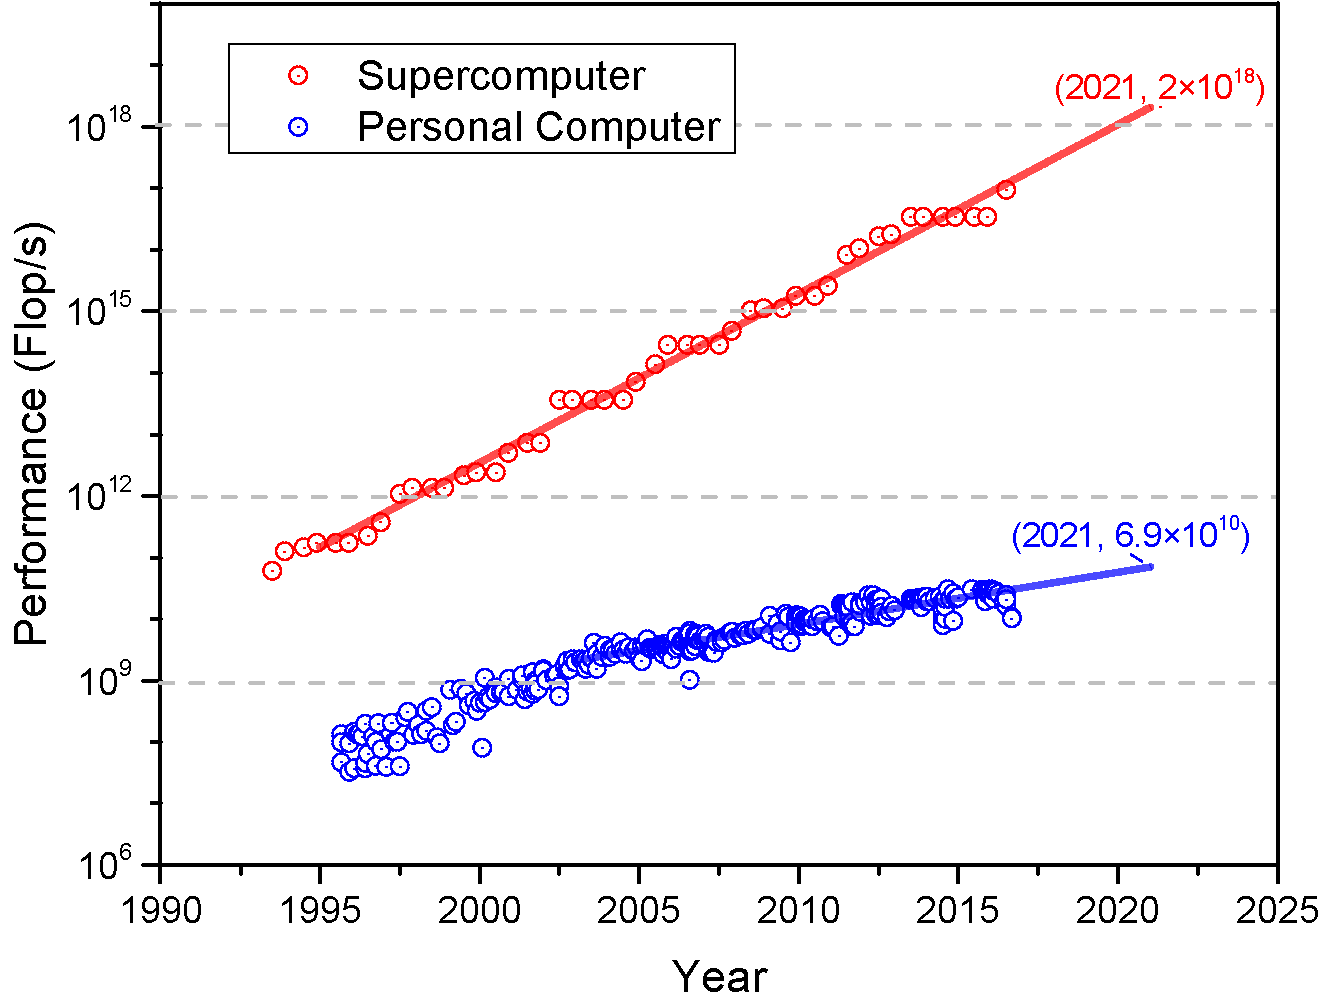
\includegraphics[width=\columnwidth]{moores_law}
\caption{Historical trends in classical computing power for both PC's and top-end supercomputers, with an extrapolation 5 years into the future. The close fit to exponential growth in performance over time is apparent.} \label{fig:moores_law}
\end{figure}

As a comparison we compare this to the {\sc BosonSampling} (Sec.~\ref{sec:BS}) model for restricted quantum computation, as it is perhaps the most plausible candidate for the first demonstration of quantum computational supremacy. The relationship between {\sc BosonSampling} photon-number and classical equivalent processing power is shown in Fig.~\ref{fig:moores_super}.

\begin{figure}[!htb]
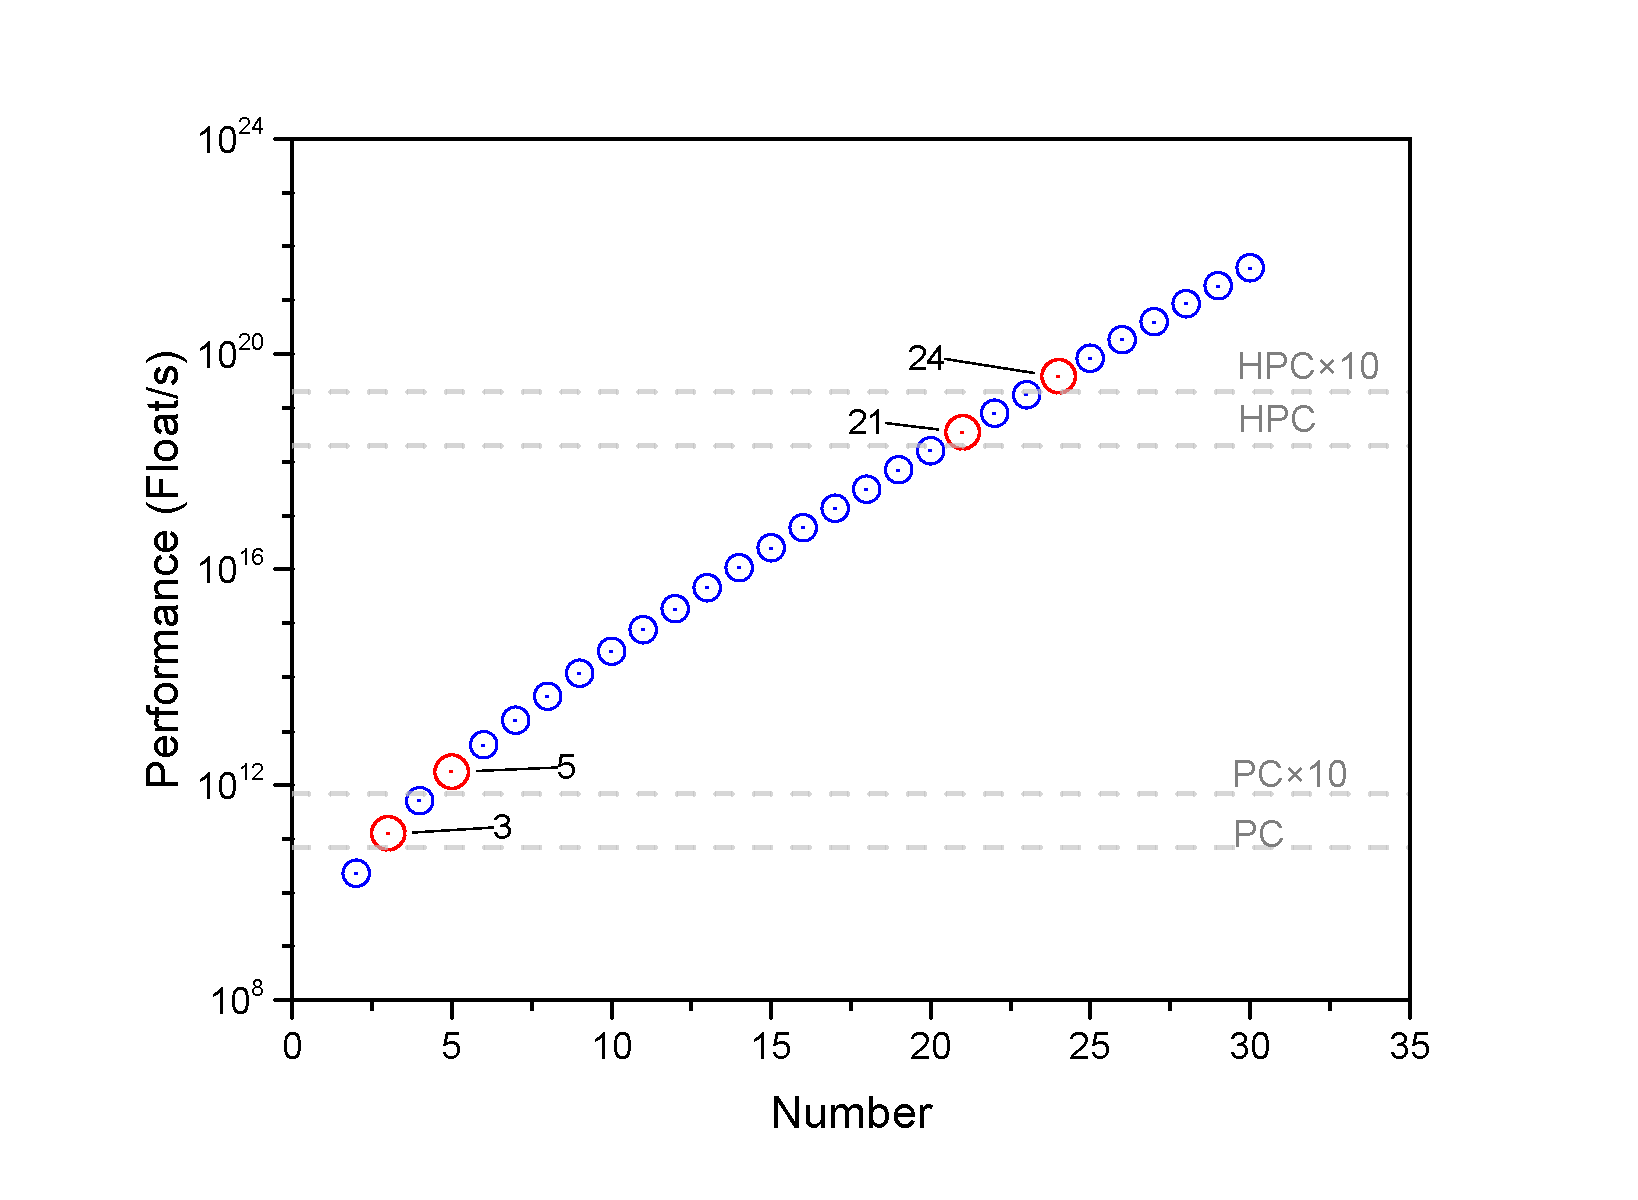
\includegraphics[width=\columnwidth]{moores_super}
\caption{Relationship between photon-number and classical equivalent FLOPS for `scattershot' {\sc BosonSampling}. The annotated red data-points show several points of interest, taking a Moore's Law extrapolation of classical computing power 5 years into the future for desktop PC's and top-end high-performance computers, as well as an order of magnitude greater performance respectively. We use these as indicators of the post-classical era.} \label{fig:moores_super}
\end{figure}

Based on these extrapolations, \cite{CYLu} made the prediction that a {\sc BosonSampling} computer could outperform top-end supercomputers of 5 years into the future by an order of magnitude (a fairly reasonable benchmark for usage of the term `post-classical') using just \mbox{$\sim 24$} photons. Given that present-day experimental efforts have recently reached 10 photons \cite{bib:tenPhotEnt}, with great ambitions to scale up further, it is to be expected that the post-classical era is imminent. Whilst it is difficult to predict exactly when technology will allow a bank of 24 high-fidelity, highly-indistinguishable, push-button (or heralded) single-photon sources operating in parallel, it seems fair to predict that the timescale will be on the order of years rather than decades.

However, be weary that we are being a little optimistic with this statement, since {\sc BosonSampling} is not universal for quantum computation, and doesn't even have any known practical uses, i.e it's post-classical and that's about it! It would be more helpful to consider prospects for \emph{universal} quantum computation.

While the power of classical computers scales at most linearly with the number of transistors, the classical-equivalent power of quantum computers scales exponentially with the number of qubits (in the best-case scenario). The classical Moore's Law is close to saturation -- we simply can't make transistors too much smaller than they already are\footnote{Current transistor feature sizes are on the order of several hundred atoms. Under a Moore's Law prediction, we are likely to hit fundamental physical barriers in transistor size within a decade.}! We therefore envisage a new Quantum Moore's Law, which follows a far more impressive trajectory than its classical counterpart. The point of critical mass in quantum computing will take place when the classical and Quantum Moore's Law extrapolations intersect, signalling the commencement of the \emph{post-classical era}. Estimating this is more challenging than it sounds, since although the classical Moore's Law is extremely well established with an excellent fit to an exponential trajectory, there aren't yet enough data-points to make a confident prediction about a Quantum Moore's Law, to what trajectory it best fits, and at what rate it progresses.

On the other hand, aside from quantum computing, QKD systems are already technologically viable, and are in fact commercially available off-the-shelf today, as end-to-end units connected via fibre-optics. As the era of post-classical quantum computation edges closer, the importance of QKD networks will intensify, and along with it the demand for quantum networking infrastructure.

It is clear that humanity already sits at the precipice of harnessing quantum technologies, and must act quickly to enable them to be fully exploited as they emerge in the near future.

%
% The Economics of the Quantum Internet
%

\section{The economics of the quantum internet} \label{sec:economics}

Quantum computers are highly likely to, at least initially, be extremely expensive, and affordable outright by few. Thus, client/server economic models based on outsourcing of computations to servers on a network, will be essential to making quantum computing widely accessible. The protocols we have presented here pave the way for this type of economic model to emerge. It is paramount that the types of technologies introduced here be fully developed in time for the deployment of useful quantum computing hardware, such that they can be fully commercialised from day one of their availability, enabling widespread adoption, enhanced economy of scale, and rapid proliferation.

A key question regarding the economics of the quantum internet is the extent to which it will be able to piggyback off existing optical communications infrastructure, given that networking will almost inevitably be optically mediated. We have an existing intercontinental fibre-optic backbone, as well as sophisticated satellite networks. To what extent will this existing infrastructure (or future telecom/satellite infrastructure) be able to be exploited so as to avoid having to rebuild the entire future quantum internet infrastructure from scratch? This is a question worth tens of billions of dollars. We also need to factor in that given the massive driving force behind telecom technology, its cost is following a Moore's Law-like trajectory, and what costs a billion dollars today might cost a million dollars in a decade's time. In light of this, telecom wavelength quantum optics is being hotly pursued. And at the time of writing this paragraph, a world-leading Chinese experimental team has just successfully launched a QKD satellite into low Earth orbit \cite{???}, enabling intercontinental entanglement distribution and QKD, with talk of the next space race being the one for quantum supremacy \cite{???}.

Technology should benefit humanity, not only an elite few. In light of this, who exactly will benefit from the quantum internet? Its beauty is that it doesn't create a system of winners and losers. Rather, it establishes a technological infrastructure from which all can benefit, rich or poor. Well-resourced operators who can afford quantum computers, for example, will benefit from being able to license out compute time on their computers, ensuring no wasted clock-cycles and maximising efficiency. The less-well-resourced will benefit in that they will have a means by which to access the extraordinary power of quantum computing on a licensed basis, facilitating access to infrastructure by those who otherwise would have been priced out of the market. This is essentially the same model as what is employed by some present-day supercomputer operators, enabling small players access to supercomputing infrastructure. The quantum internet is critical to achieving the same goal in the quantum era. This could have transformative effects on the developing world in particular. And many emerging industries, for whom access to quantum computation will be critical, but who cannot afford them, will benefit immensely from the client/server model.

Already today, even before the advent of useful post-classical quantum computers, we are seeing the emergence of the outsourced model for computation. IBM recently made an elementary 5-qubit quantum computer freely available for use via the cloud. Interested users can log in online, upload a circuit description for a quantum protocol, and have it executed remotely, with the results relayed back in real-time. Although still very primitive, this simple development already makes experimentation with elementary quantum protocols accessible to the poor layman, undergrad, or PhD student in a developing country, people who just last year would never have dreamt of being able to run their own quantum computing experiments! This effectively opens up research opportunities to people who otherwise would have been priced out of the market entirely, unable to compete with established, well-resourced labs. Evidently, the market already recognises the importance of outsourced models for quantum computation. We encourage the impatiently curious reader to log onto the `IBM Quantum Experience' ({\tt \href{http://www.research.ibm.com/quantum/}{http://www.research.ibm.com/quantum/}}) and take a shot at designing a 5-qubit quantum protocol, without even seeing the quantum computer.

The quantum internet will facilitate the communication and trade of quantum assets beyond just quantum computation and cryptography. There are many uses for various hard-to-prepare quantum states, for example in metrology, lithography, or research, where outsourcing state preparation would be valuable. Alternately, performing some quantum measurements can be technologically challenging, and the ability to delegate them to someone better-equipped would be desirable. The quantum internet goes beyond just quantum computing. Rather, it extends to a full range of quantum resources and protocols.

To commodify quantum computing, if constructing large-scale quantum computers were a simple matter of plug-and-play, where QuantumLego\texttrademark \,building blocks are available off-the-shelf and straightforward to assemble even for monkeys, mass production would rapidly force down prices. By arbitrarily interconnecting these boxes, large-scale quantum computers could be scaled up with demand, with a trajectory following a new Quantum Moore's Law, and a price scaling linearly with the number of qubits. We envisage that each of these commodity items is a black box, within which a relatively small number of qubits are held captive. Then, to build a larger quantum computer, we don't need to upgrade our boxes. Rather, we simply purchase more boxes to interconnect over the network. This notion is tailored to cluster states in particular -- because a cluster state can be realised by nearest neighbour interactions alone, and since all preparation stages commute with one another, they naturally lend themselves to modularised, distributed preparation.

On the other hand, if quantum computers were only ever sold as specialised, room-sized, all-in-one solutions (think D-Wave), such mass production would not experience the driving force of commodified, off-the-shelf building blocks, each of which is cheap, yet frugal in its computational power alone.

Taking the concept of distributed computation to the logical extreme, modularised quantum computation mitigates the need to purchase large-scale quantum computers outright, allowing them to be gradually scaled up as demand increases and production costs diminish. Additionally, they can be shared across multiple users, with the economic benefit of maximising resource utilisation, and the practical benefit of the end-user effectively having a much larger quantum computer at their disposal. By having a standardised architecture for optically interconnecting modules, we also somewhat `future-proof' our hardware investment -- if interfacing modules is standardised, existing hardware can be fully compatible with newer, more capable module versions. 

%
% Security Implications of the Global Quantum Internet
%

\section{Security implications of the global quantum internet} \label{sec:sec_imp}

With any new technology comes ethical considerations. Who will have access to it, and how do they plan to use it? For this reason, many developed nations have export bans or restrictions in place on `dual-use' technologies -- those which have clearly legitimate and morally justifiable uses, but also nefarious ones by competitors and criminals. Nuclear technology is the obvious archetype. Quantum technologies (in particular quantum computing and quantum cryptography) are particularly vulnerable to dual-use, and for this reason are becoming subject to dual-use technology legislation, such as export controls, in some nations. In Australia, for example, legislation is being introduced criminalising the transfer of knowledge on certain quantum and cryptographic technologies to foreign nationals of certain target countries.

With a global QKD infrastructure in place, any person on Earth would have uncrackable encryption at their fingertips. Whilst this might be welcomed by the populace of a despotic regime (or the libertarians in a democratic one), it would clearly be unwelcome for that level of secrecy and protection to be awarded to the regime itself. Similarly, criminal and terrorist organisations would be immune to government surveillance. With widespread global adoption of QKD technology, the signals intelligence agencies of nation states would become entirely obsolete, leaving the NSA and its Five Eyes\texttrademark \,partners furious.

Quantum computing also has dual-use potential. In fact, given their ability to compromise some existing cryptographic protocols, it appears highly likely that the first useful, post-classical quantum computers will find their way into the hands of national SIGINT agencies. Of course, it doesn't take much imagination to see that many other quantum algorithms could be employed for sinister purposes. For this reason we are likely to see export limitations placed on quantum computer technology in the future.

Much as the internet has eliminated national electronic borders, a quantum internet employed for distributed or outsourced computation, would make quantum computer technology available to hackers, criminals, terrorists, and strategically competing nations. And a distributed model for computation as unregulated as the classical internet would make it near impossible to prevent.

Combined with encrypted quantum computing protocols, no one would even know what they were up to when using this awesome computing power, and what they learn, they could keep to themselves. Alg.~\ref{alg:russian} describes a typical protocol for a particularly nefarious application for this.

\begin{table}[!htb]
\fbox{\parbox{0.965\columnwidth}{\tt
function MakeAmericaGreatAgain(Putin):
\begin{enumerate}
    \item A Russian bedroom hacker with no direct access to quantum technology, delegates a factorisation algorithm to the cloud using homomorphic encryption.
    \item The computation is physically executed on a server in the United States.
    \item The result in returned to our Russian comrade.
    \item The Russian uses the obtained private RSA key to hack Hillary's emails.
    \item The emails are strategically leaked during the next Presidential election.
    \item This swings the election in favour of Trump\texttrademark.
    \item The NSA and FBI have no clue who was behind it, since it was homomorphically encrypted.
    \item They blame Edward Snowden.
    \item Fox News\texttrademark \,calls for his execution.
    \item They'd kick themselves if they found out the algorithm was actually executed on US soil.
    \item Unless the NSA switches off the entire quantum internet, they can't prevent it from happening again in subsequent elections.
    \item return(America is Great Again\texttrademark).
    \item $\Box$
\end{enumerate}}}
\caption{A typical example of a nefarious use for cloud quantum computation.} \label{alg:russian}
\end{table}

These are all legitimate concerns. But they are very much the same ones that detractors expressed about the classical internet and strong encryption. Nonetheless, it can be said that encryption and the internet have on balance been overwhelmingly beneficial to mankind, enabling unprecedented rates of technological progress. Any attempts to eliminate or undermine them could be economically catastrophic.

We take the view that the same ethical stance ought to be applied in the quantum era. While quantum technologies clearly have dual-use potential, the magnitude of the implications they will have for scientific and technological progress overwhelms the discussed proliferation issues. No doubt, politicians will nonetheless attempt to regulate and restrict the quantum internet -- that's what governments like to do. But this will inevitably fail for the same underlying reasons that it failed for the classical internet -- no tech-savvy Chinese person can actually say they are hindered by the Great Firewall of China\texttrademark.

%
% The Vision of the Global Quantum Internet
%

\section{The vision of the global quantum internet} \label{sec:vision_quant}

Quantum technologies, particularly quantum computing, will truly revolutionise countless industries. With early demonstrations of key quantum technologies -- such as QKD, long distance quantum teleportation, and quantum computing -- becoming a reality, it is of utmost importance that networking protocols be pursued.

We have presented an early formulation and analysis of quantum networking protocols with the vision of enabling a future quantum internet, where quantum resources can be shared and communicated in much the same way as is presently done with digital assets. Whilst it is hard to foresee exactly how future quantum networks will be implemented, many of the central ideas presented here will be applicable across architectures and implementations on an ad hoc basis.

There are a number of schools of thought one might subscribe to when quantum networking. One might demand perfect data integrity and best-case network performance. But that would come at the expense of necessitating an all-powerful central authority to oversee all communications, ensuring that scheduling was absolutely perfect -- a potentially very challenging optimisation problem. Or one might tolerate lost data packets or suboptimal performance, but at the expense of limiting the applicability of the network. Or maybe some arbitrary compromise between different metrics and attributes is best. These are open questions that needn't have concrete, one-size-fits-all answers.

The QTCP framework we presented is sufficiently flexible and extensible that these questions can be answered and enforced independently by different subnets, depending on their individual characteristics and requirements, in much the same way that every organisation connected to the classical internet today is free to structure their own LAN as they please, enforcing their own network policies.

The quantum internet will allow quantum computation to become distributed, not just outsourced. In the same way that many present-day classical algorithms are heavily parallelised and distributed across large clusters, CUDA cores, or even across the internet itself (e.g the SETI project), quantum networks will allow the distribution of quantum computation across many nodes, either in parallel, in series, or in a modularised fashion. This will be pivotal to achieving scalability. Keeping in mind that the classical-equivalent power of a quantum computer may grow exponentially with the number of qubits, it is highly desirable to squeeze out every last available qubit for our computations -- every qubit is worth more than the last.

Combined with recent advances in homomorphic encryption and blind quantum computation, commercial models for the distribution of quantum computation will emerge, allowing computational power to be outsourced, with both client and server confident in the security of their data and proprietary algorithms. This is a notion that is challenging on classical computers, but will be of utmost importance in quantum computing, where it is expected sensitive data and algorithms will often be at stake.

From the security perspective, the global quantum internet will enable an international QKD communications network with perfect secrecy, guaranteed to be information-theoretically secure by the laws of physics. This will be of immense economic and strategic benefit to commercial enterprises, governments, and individuals. Classical cryptography is already a multi-billion dollar industry worldwide. Quantum cryptography will supersede it, and be of especial importance in the era of quantum computers, which compromise some essential classical cryptographic protocols, such as RSA, which forms the basis of most current internet encryption, digital signatures, and the Blockchain/Bitcoin protocols. Not only is quantum cryptography being pursued optically, but even credit cards with embedded quantum circuitry are being actively developed to prevent fraud. Inevitably, this will require the communication between bank automats and servers to be mediated by a quantum network.

Already, off-the-shelf QKD systems are available as commodity items, from vendors such as MagiQ and ID Quantique, which may be simply interconnected via an optical fibre link, thereby implementing end-to-end quantum cryptography. This is of a similar flavour to, and first technological step towards, modularised quantum computing, which would greatly enhance the economic viability and scalability of general purpose quantum computing by paving the way for the mass production of elementary interconnectable modules as commodity items.

We have focussed our attention thus far on the application of quantum networking to quantum information processing applications, such as quantum computing and quantum cryptography. However, with plug-and-play quantum resources available over a network, one might envisage far greater applicability than just these.

Of particular interest is the implications of quantum networking to basic science research. Presently, experimental quantum physics research is limited to well-resourced labs with access to state of the art equipment. With the ability to license these assets over a network, and interconnect them on an ad hoc basis, the ability to construct all manner of quantum experiments could be extended to all. An undergraduate laboratory would now have the ability to approach a host to politely borrow their state engineering technologies, send it to another with the ability to perform some evolution to that system, and to yet another to perform measurement and analysis of the output -- all from an undergrad lab equipped with nothing more than desktop computers. This has broad implications for basic science research, opening it up to aspiring researchers across the globe, regardless of their direct access to cutting-edge tools. This will greatly expand the intellectual base for conducting quantum experimentation to the entire global scientific community, destroying the scientific monopolies controlled by a handful of world-leading experimental groups.

The reality is that we are only just beginning to understand the full potential for quantum technologies, and as we learn more we will inevitably find new uses for networking them.

Large-scale quantum computing may still seem a formidable, and somewhat long-term challenge. But it isn't likely to remain so. Once we have mastered the technological art of preparing qubits and implementing high-fidelity entangling operations between them, it is just a matter of sitting back and watching Gordon Moore perform his witchcraft, and scalability of quantum technology, and its rapid market-driven reduction in cost, will quickly ensue. The quantum internet will drive this rapid development by expanding both the supply and demand for access to this technology.

It is essential for the adoption and development of quantum technology, that quantum networking infrastructure be sufficiently well developed that it is ready to be deployed the minute the first useful, post-classical hardware becomes available. The proliferation of the defining technology of the 21st century depends upon it.
\\

\emph{--- Ad astra per alas porci. Scientia potentia est, im Wandel der Zeiten.}

%
% Acknowledgments
%

\begin{acknowledgments}
We acknowledge Charlotte Bridault for helpful discussions. P.P.R. is funded by an ARC Future Fellowship (project FT160100397). We thank 1,3,7-Trimethylxanthine for aiding in the motivation for this work.
\\
\\

%
% Statement of Contributions
%

\textbf{Statement of contributions}
\\
\\
P.P.R conceived and directed this project, developed the original ideas, and prepared most of the manuscript. Z.E.S and H.L.H prepared Sec.~\ref{sec:state_of_the_art}. S.I.M contributed to Sec.~\ref{sec:classical_nets}. R.L.M contributed to Sec.~\ref{sec:protocols_quant_int}. All authors played active roles in the discussions that developed this work.
\end{acknowledgments}

%
% Bibliography
%

\bibliography{quantum_internet}

\end{document} 